\chapter{The page in use, on demonstration data}\label{ch:gallery}

Every figure in this chapter was captured from the current single-file page driven by a browser, on
synthetic demonstration runs. Nothing was staged by hand: the page was given the files, told to read
them, and photographed. Each caption names the functions the view enters through, and how many
further functions are reachable from them, so a figure can be read against the records in
Chapter~\ref{ch:val-functions}.

Two sets of runs are used. The first is the thirty-two-run demonstration instrument LC-DEMO-01,
which is in control throughout. The second is scenario S9, twenty runs in which a calibrator lot
changes at run~9: the control steps and then drifts. The second set is what the alarm figures show.

\section{Coverage}

The 66 figures enter the page at 71 distinct functions. Following the calls from those entry points reaches \textbf{448} of the 563 top-level functions in the page, or 79\,\%.

The rest are not reached from a screen: they are the download and export paths, which produce a file rather than a view, the statistics helpers those paths call, and the graph renderers, which are properties of a table of definitions rather than functions called by name --- a static reading of the source cannot follow that step, although the figures in Section~\ref{sec:gal-graphs} were produced by running them.

\section{Reading the files}
\begin{figure}[H]\centering
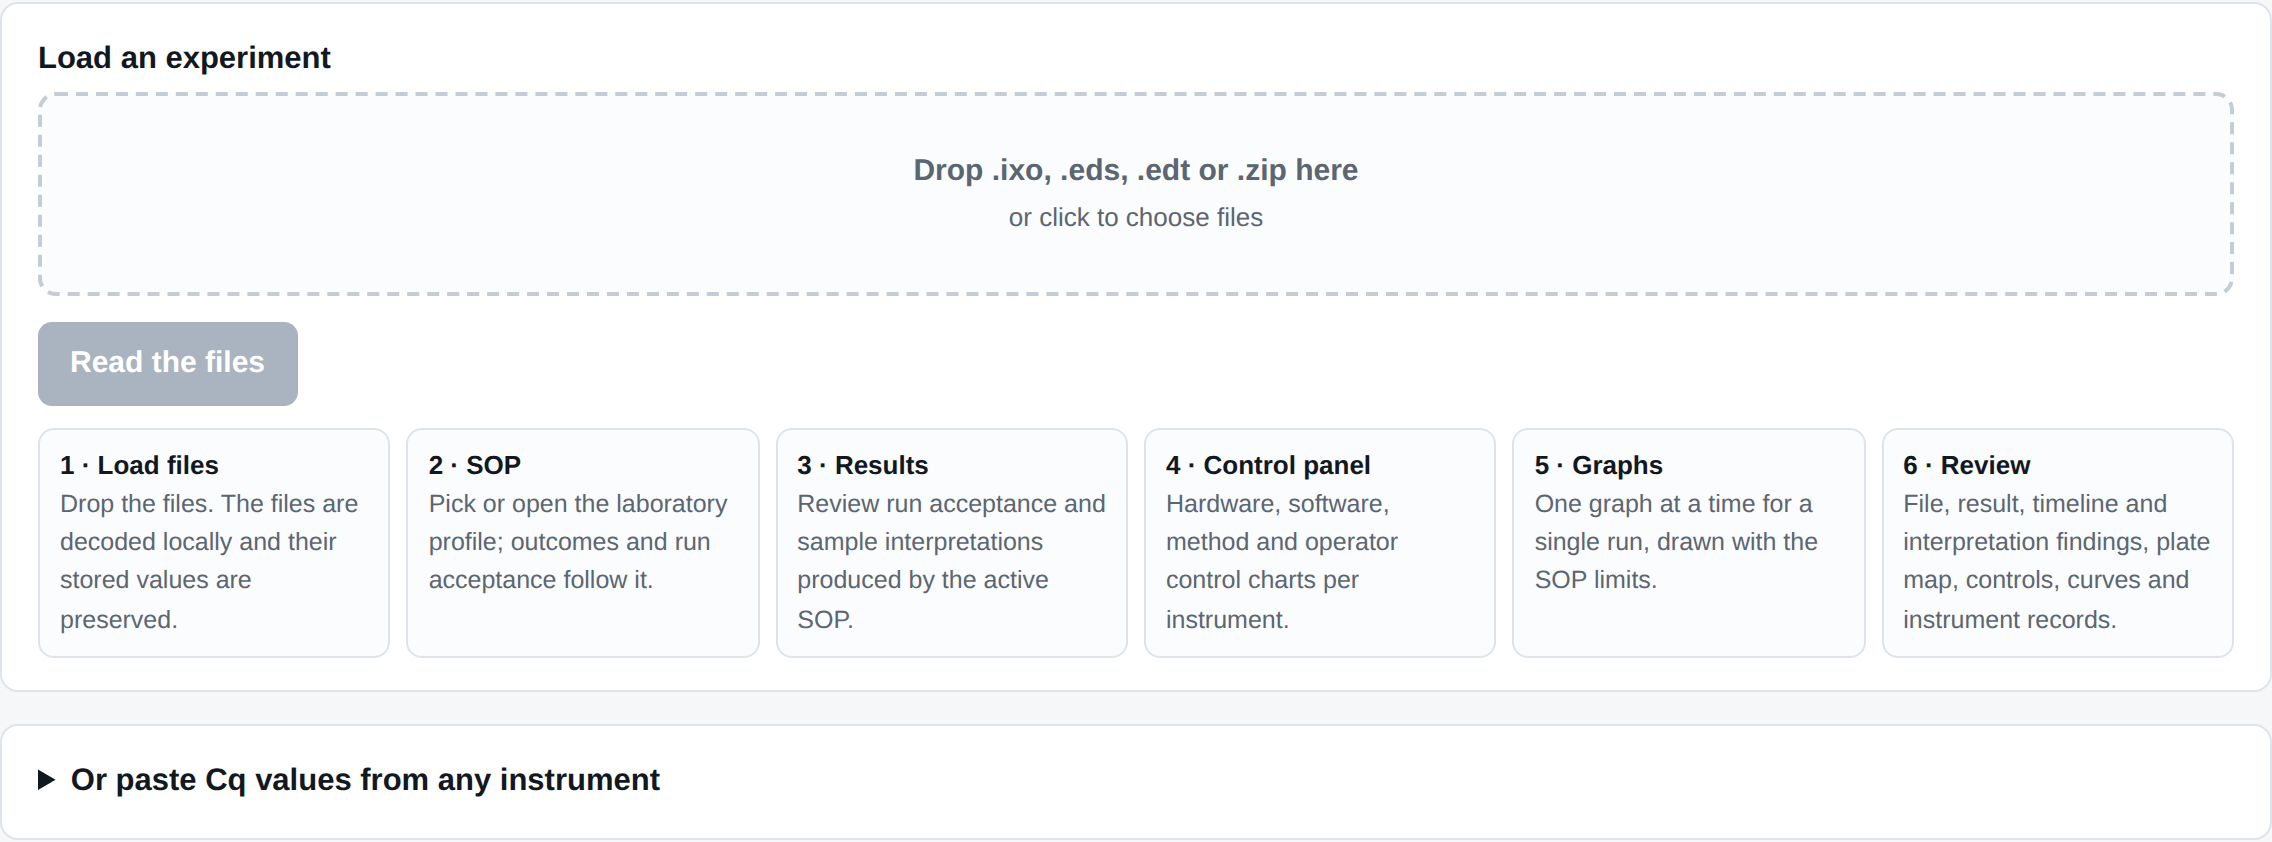
\includegraphics[width=0.96\linewidth,height=0.80\textheight,keepaspectratio]{fig/gallery/load_empty.png}
\caption[Load files, before anything is read]{\synthtag Load files, before anything is read. {\footnotesize Exercises \texttt{appNotice}, \texttt{boot}, \texttt{renderTab} and 394 more function(s) reachable from them.}}
\label{fig:gal-load-empty}
\end{figure}

\begin{figure}[H]\centering
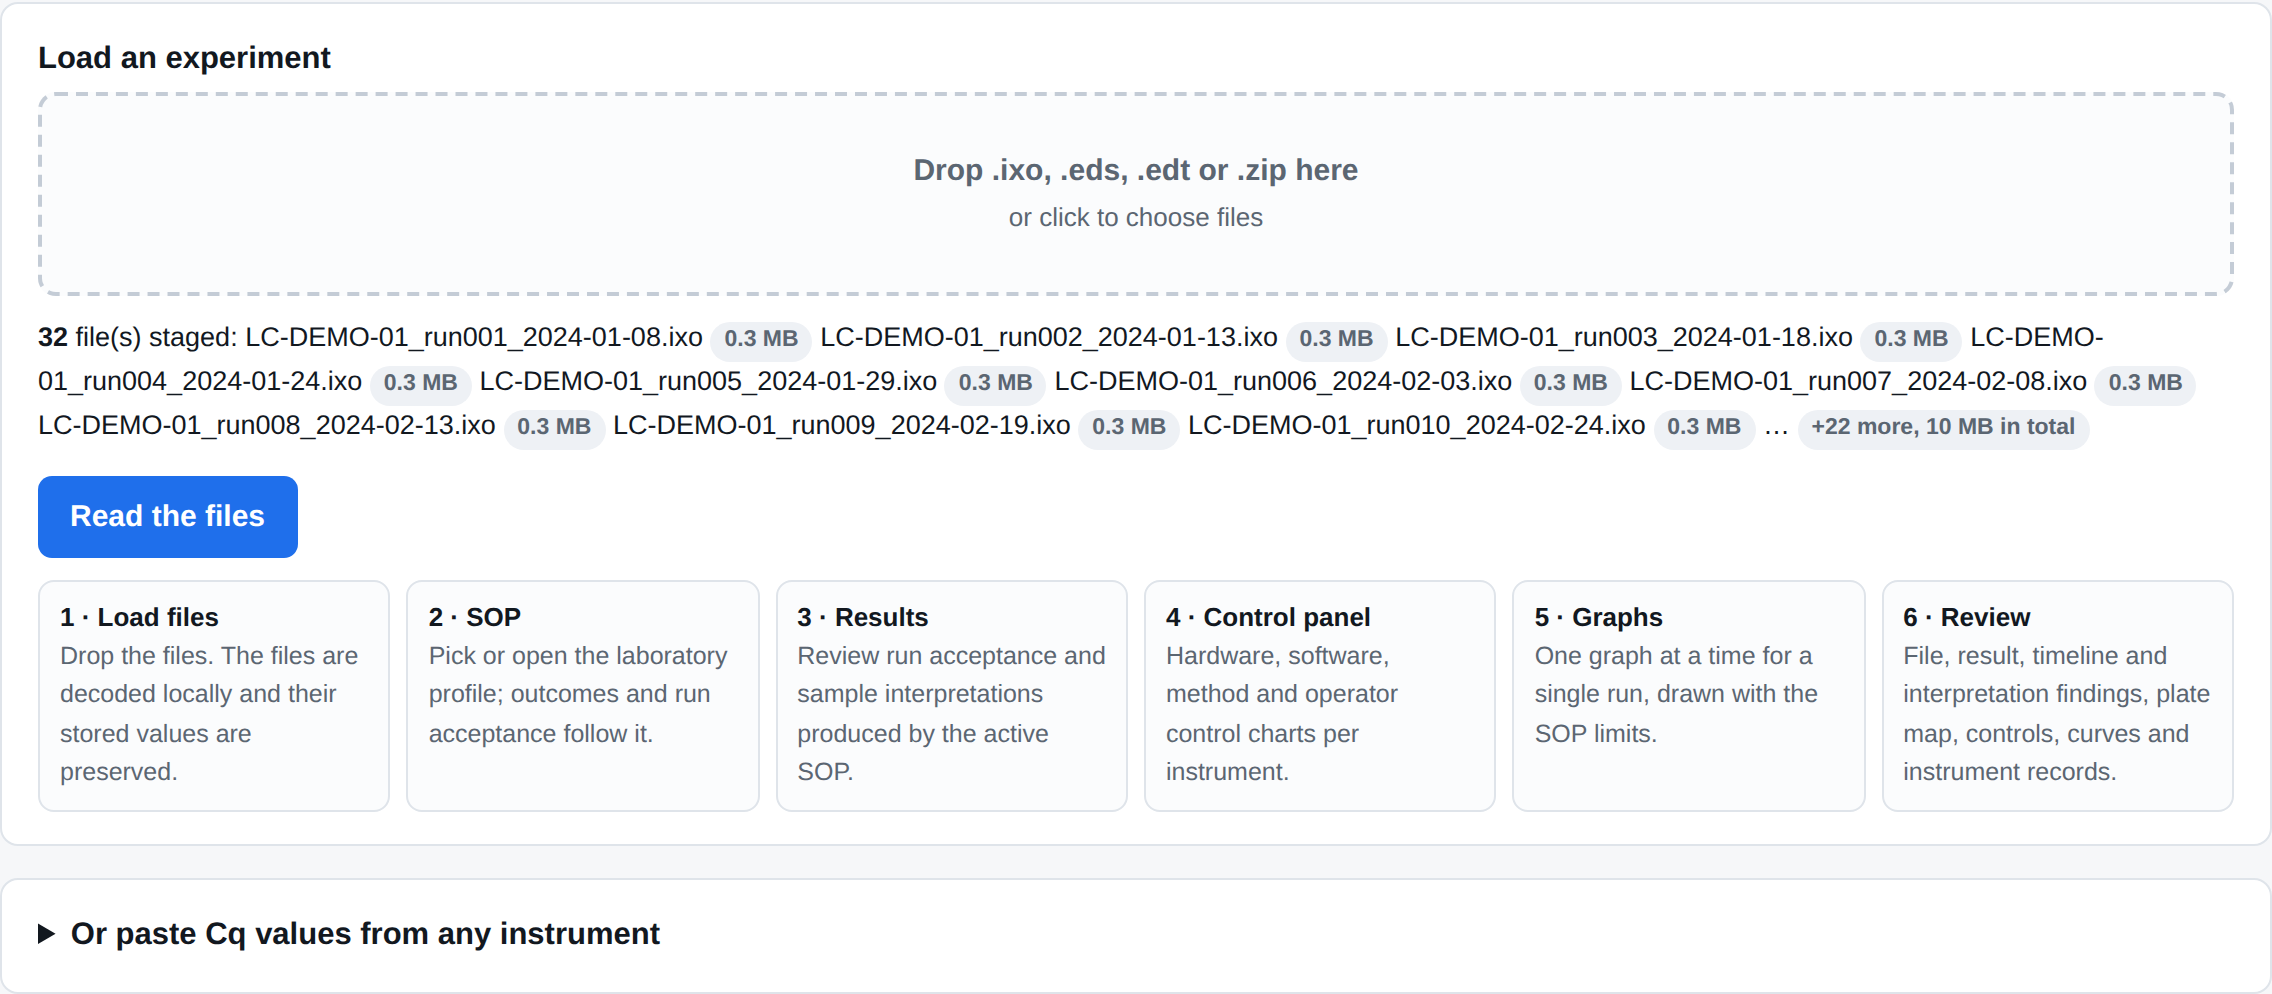
\includegraphics[width=0.96\linewidth,height=0.80\textheight,keepaspectratio]{fig/gallery/load_staged.png}
\caption[Thirty-two demonstration runs staged, not yet read]{\synthtag Thirty-two demonstration runs staged, not yet read. {\footnotesize Exercises \texttt{renderDerived}, \texttt{renderLoaded} and 28 more function(s) reachable from them.}}
\label{fig:gal-load-staged}
\end{figure}

\begin{figure}[H]\centering
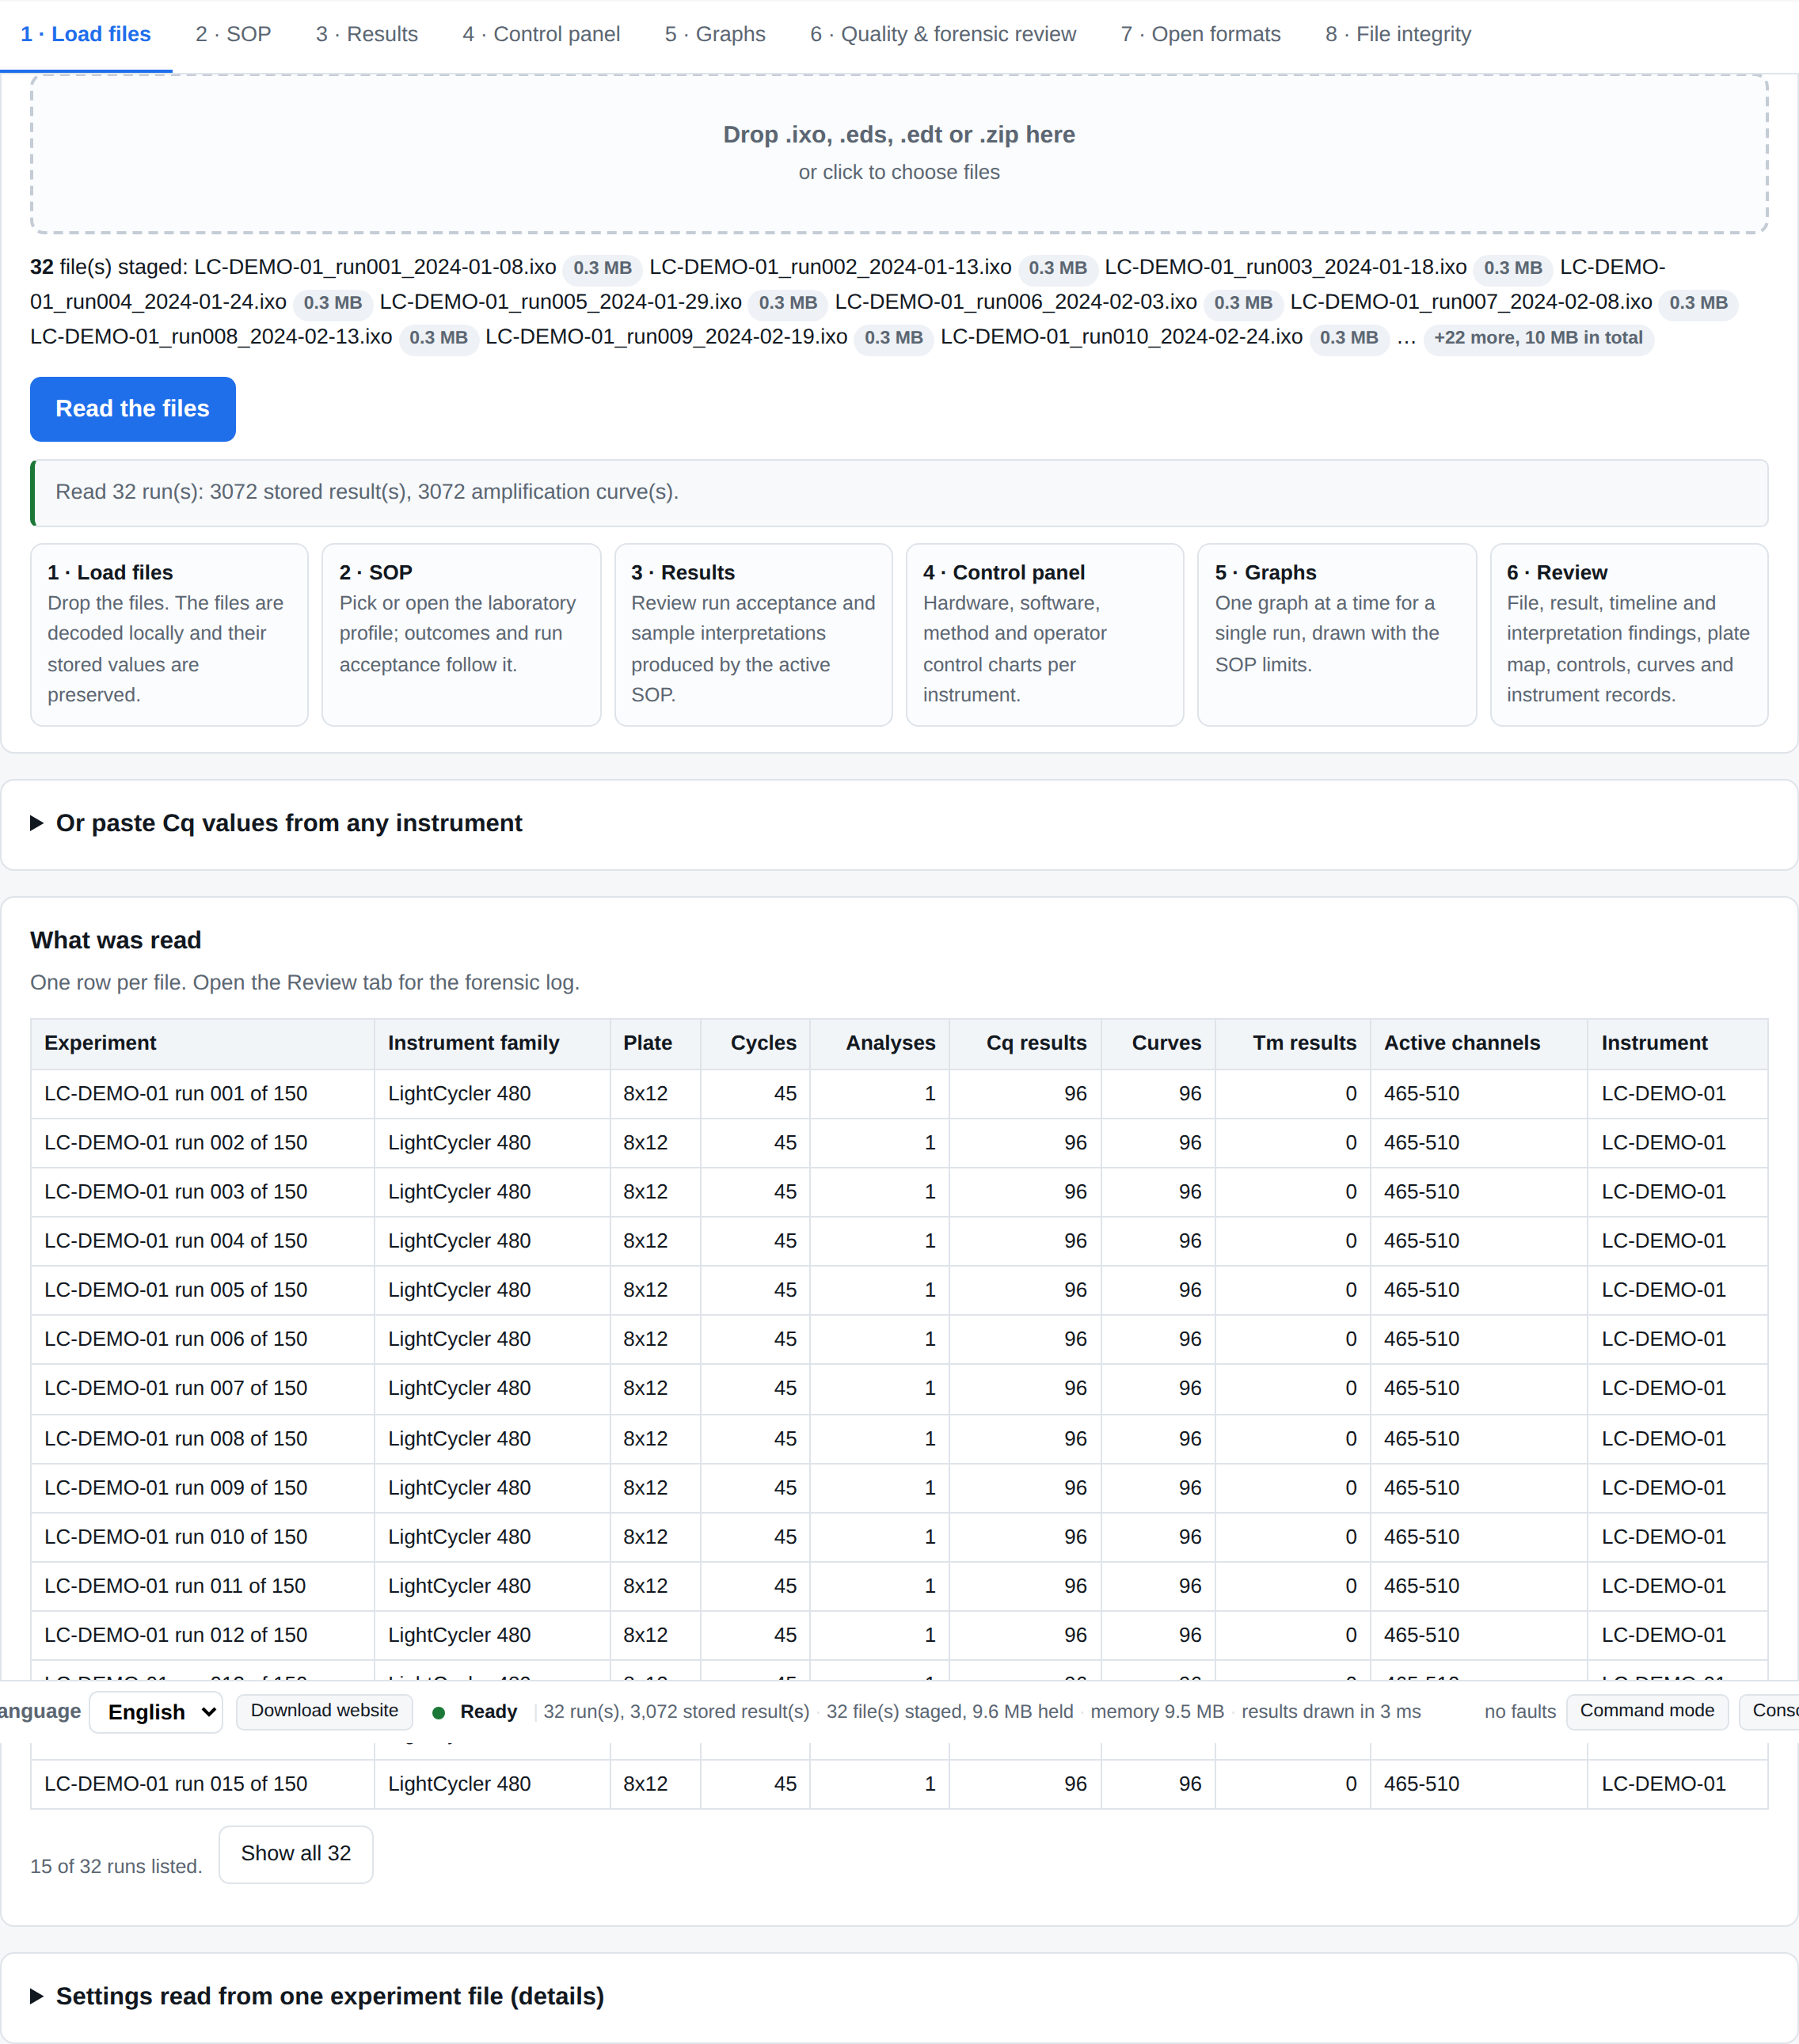
\includegraphics[width=0.96\linewidth,height=0.80\textheight,keepaspectratio]{fig/gallery/load_read.png}
\caption[The same runs after decoding]{\synthtag The same runs after decoding. {\footnotesize Exercises \texttt{decodeIxo}, \texttt{renderDerived}, \texttt{renderLoaded}, \texttt{runName} and 58 more function(s) reachable from them.}}
\label{fig:gal-load-read}
\end{figure}

\section{The tabs}
\begin{figure}[H]\centering
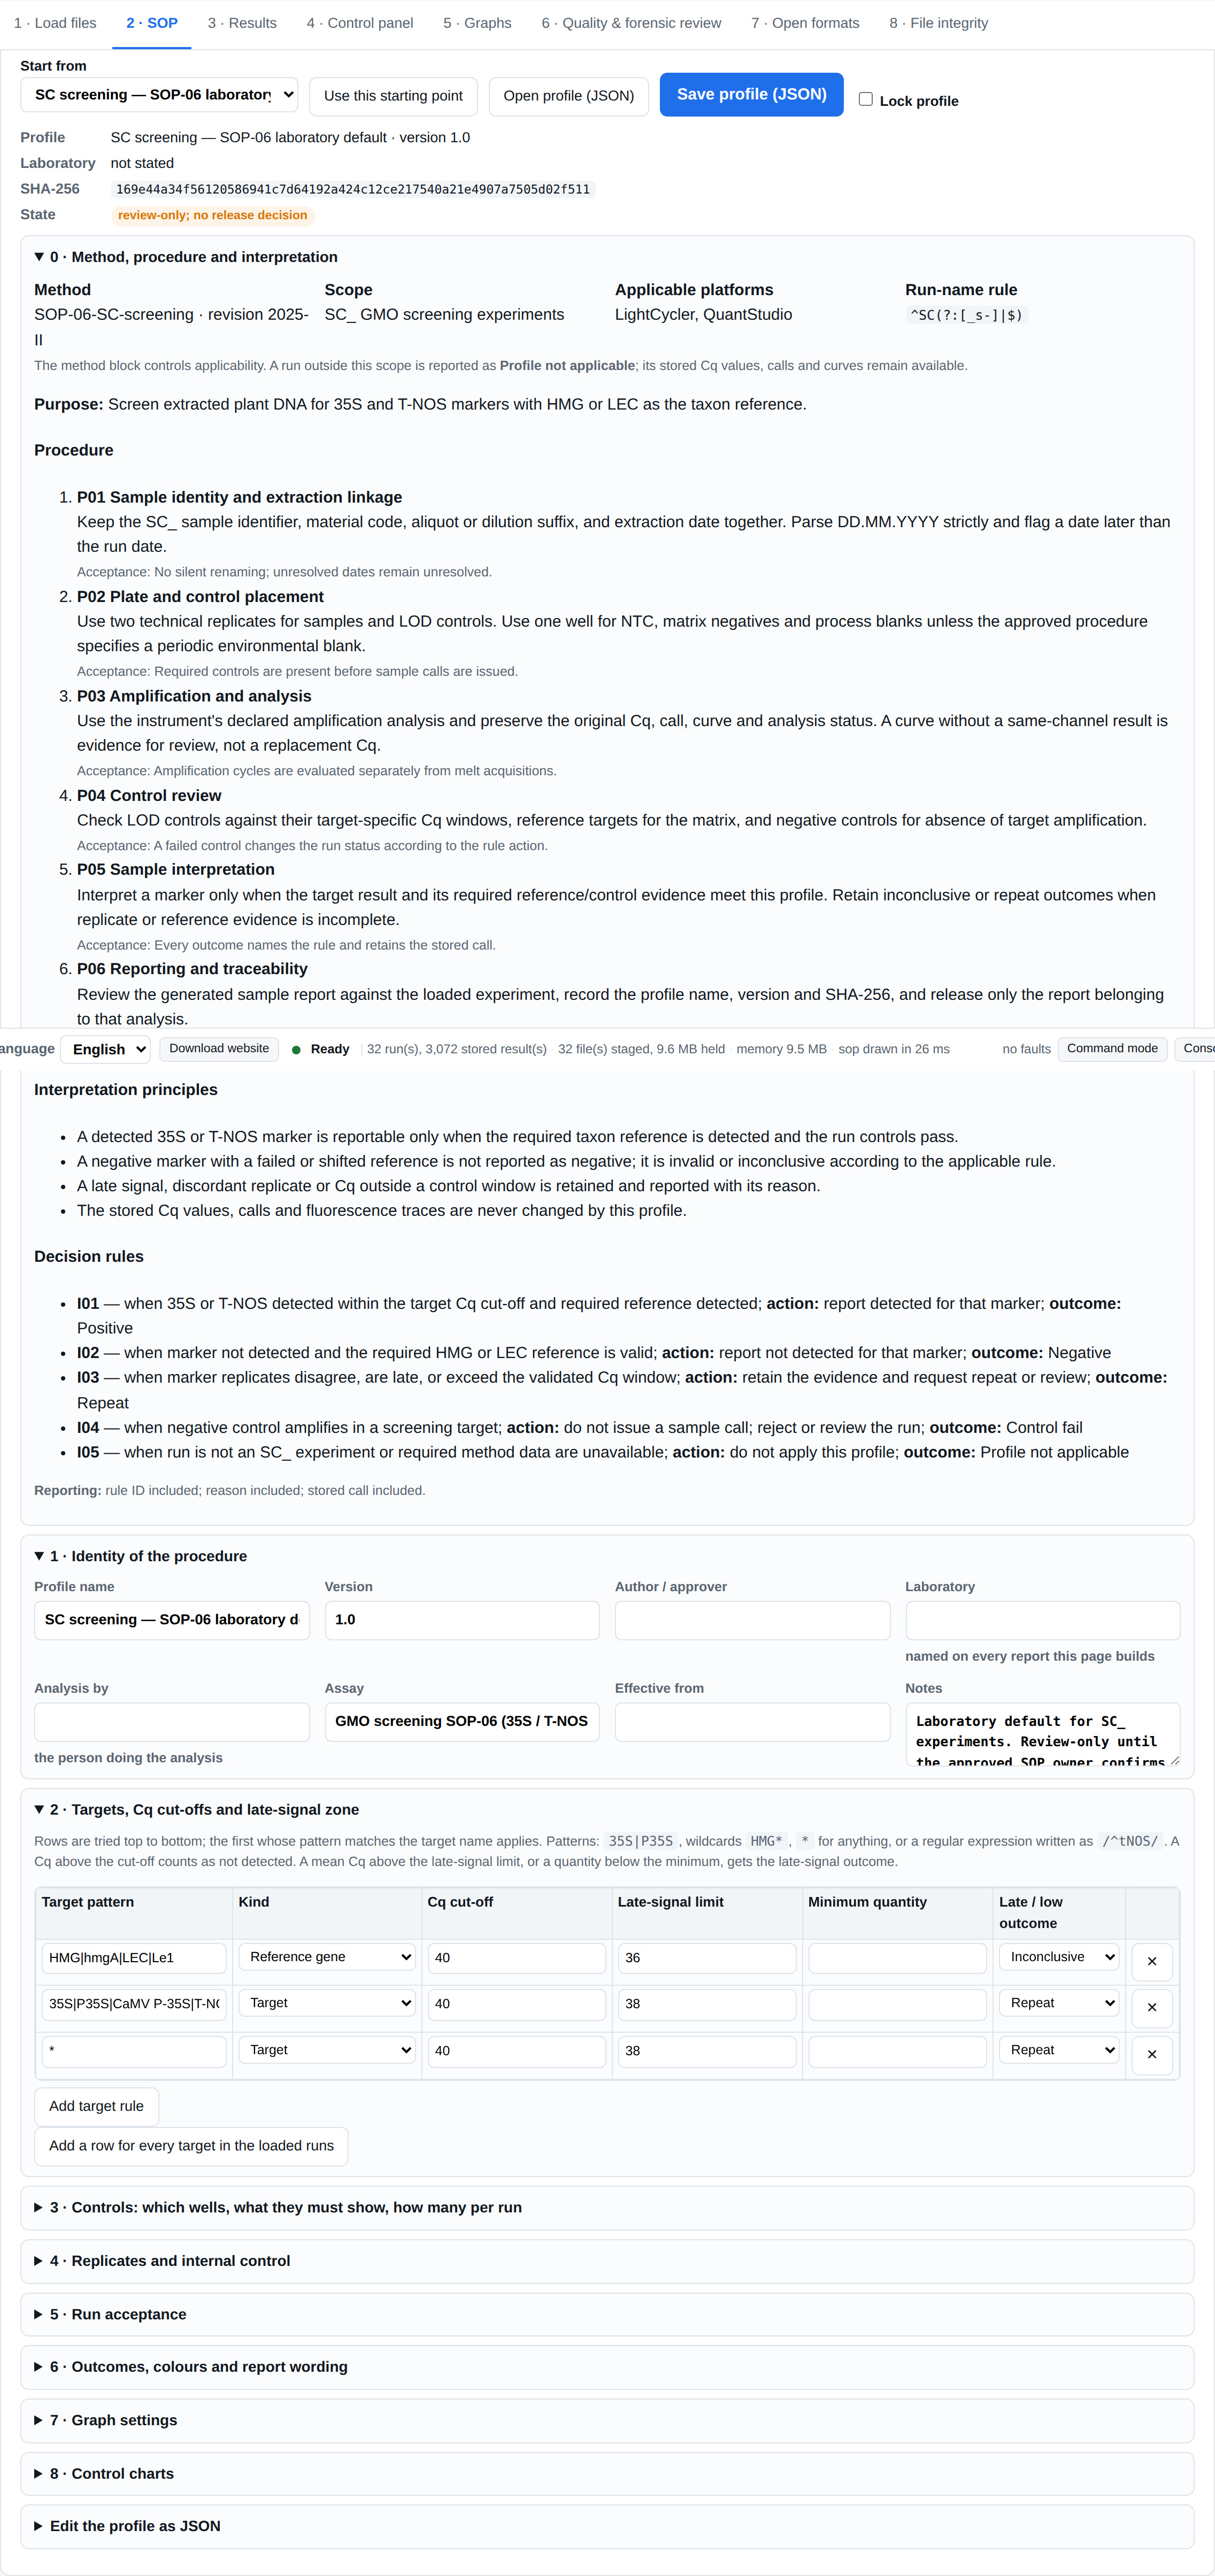
\includegraphics[width=0.96\linewidth,height=0.80\textheight,keepaspectratio]{fig/gallery/tab_sop.png}
\caption[SOP: the laboratory profile]{\synthtag SOP: the laboratory profile. {\footnotesize Exercises \texttt{renderSop}, \texttt{sopHash}, \texttt{sopNormalise} and 66 more function(s) reachable from them.}}
\label{fig:gal-tab-sop}
\end{figure}

\begin{figure}[H]\centering
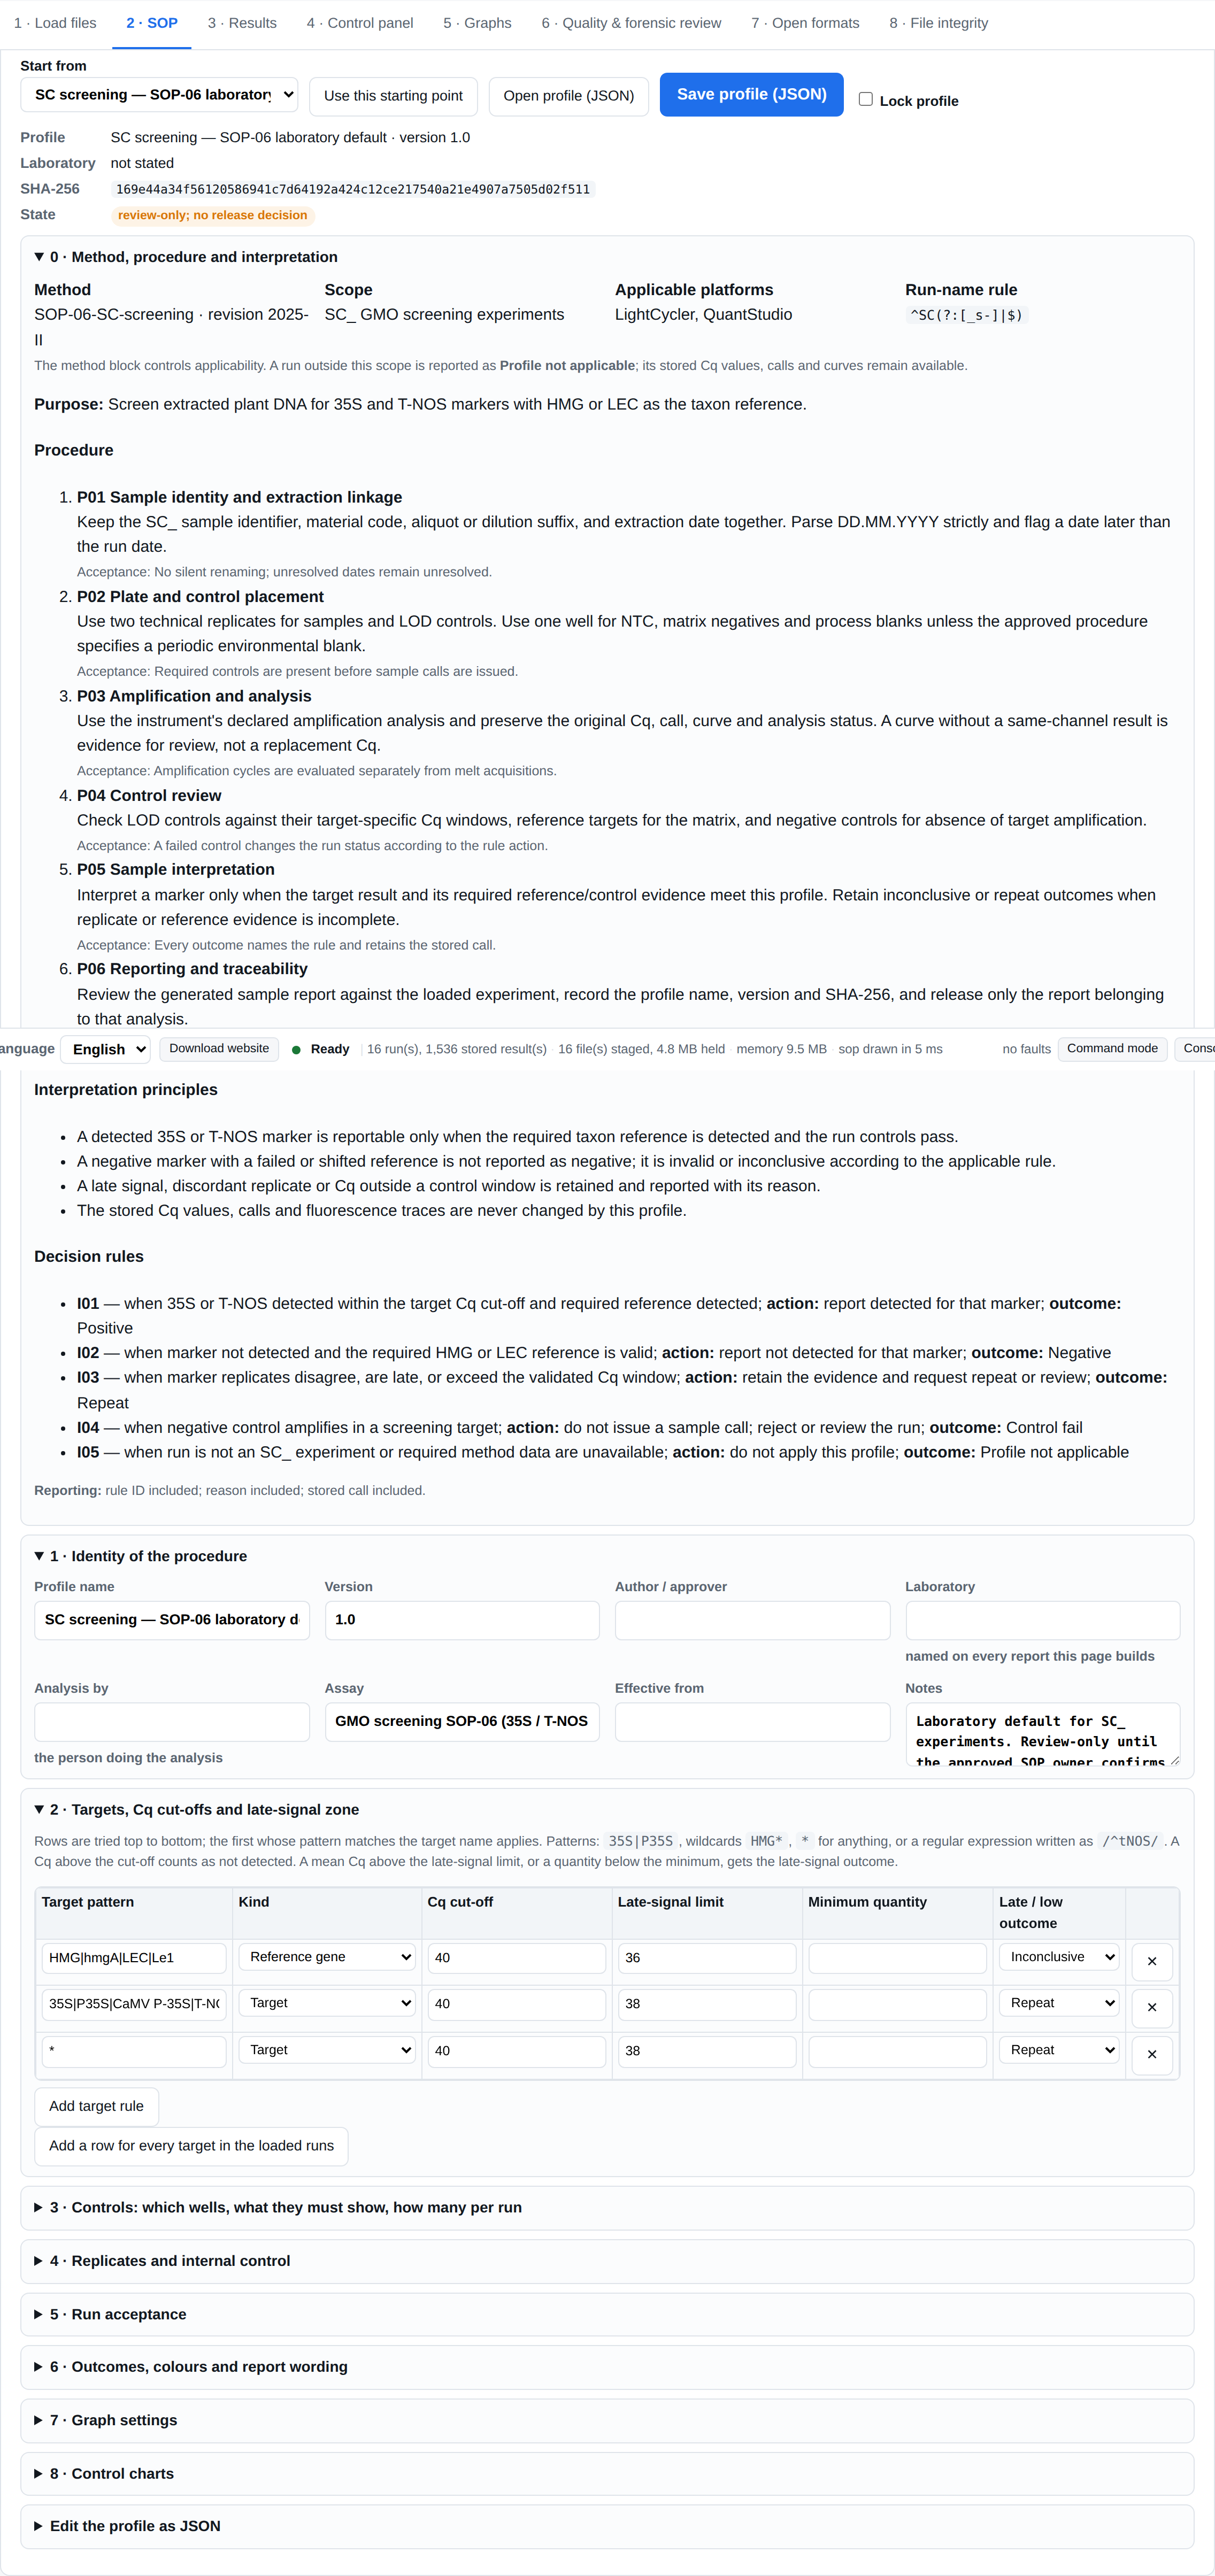
\includegraphics[width=0.96\linewidth,height=0.80\textheight,keepaspectratio]{fig/gallery/sop_editor.png}
\caption[The SOP profile: the laboratory rules the page applies]{\synthtag The SOP profile: the laboratory rules the page applies. {\footnotesize Exercises \texttt{renderSop}, \texttt{sopNormalise}, \texttt{sopTargetSpec} and 66 more function(s) reachable from them.}}
\label{fig:gal-sop-editor}
\end{figure}

\begin{figure}[H]\centering
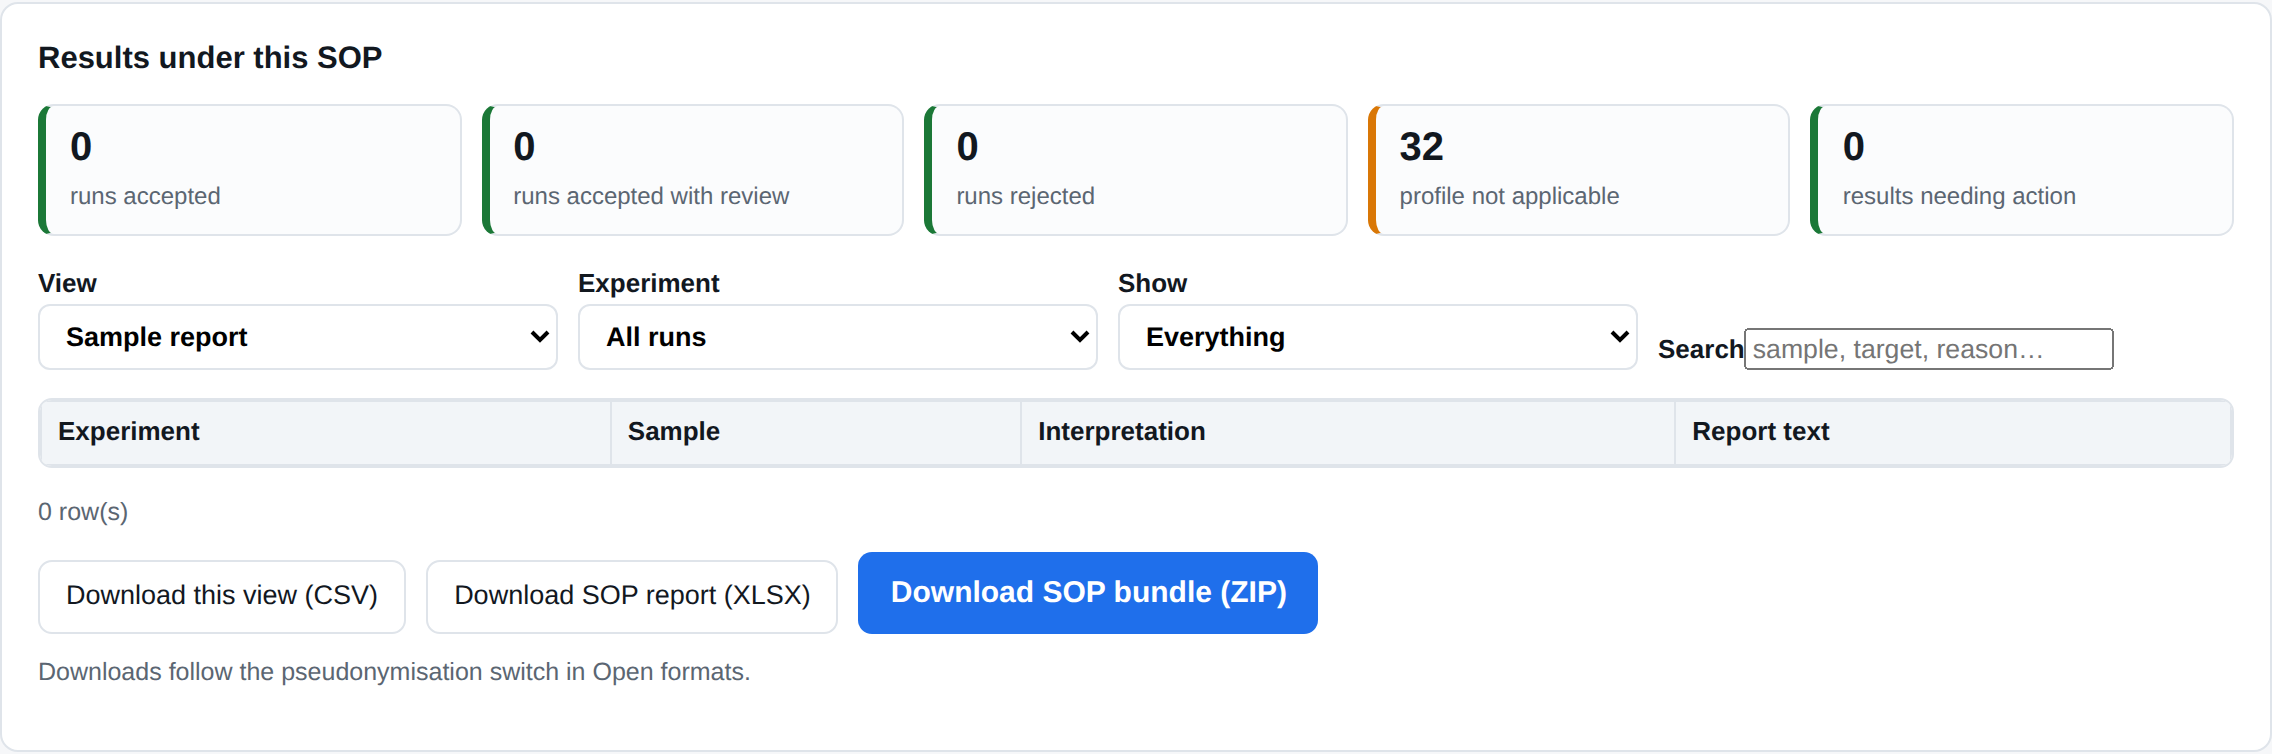
\includegraphics[width=0.96\linewidth,height=0.80\textheight,keepaspectratio]{fig/gallery/tab_results.png}
\caption[Results: stored values as the file holds them]{\synthtag Results: stored values as the file holds them. {\footnotesize Exercises \texttt{allWellRows}, \texttt{renderResults}, \texttt{reviewStatisticsRows} and 53 more function(s) reachable from them.}}
\label{fig:gal-tab-results}
\end{figure}

\begin{figure}[H]\centering
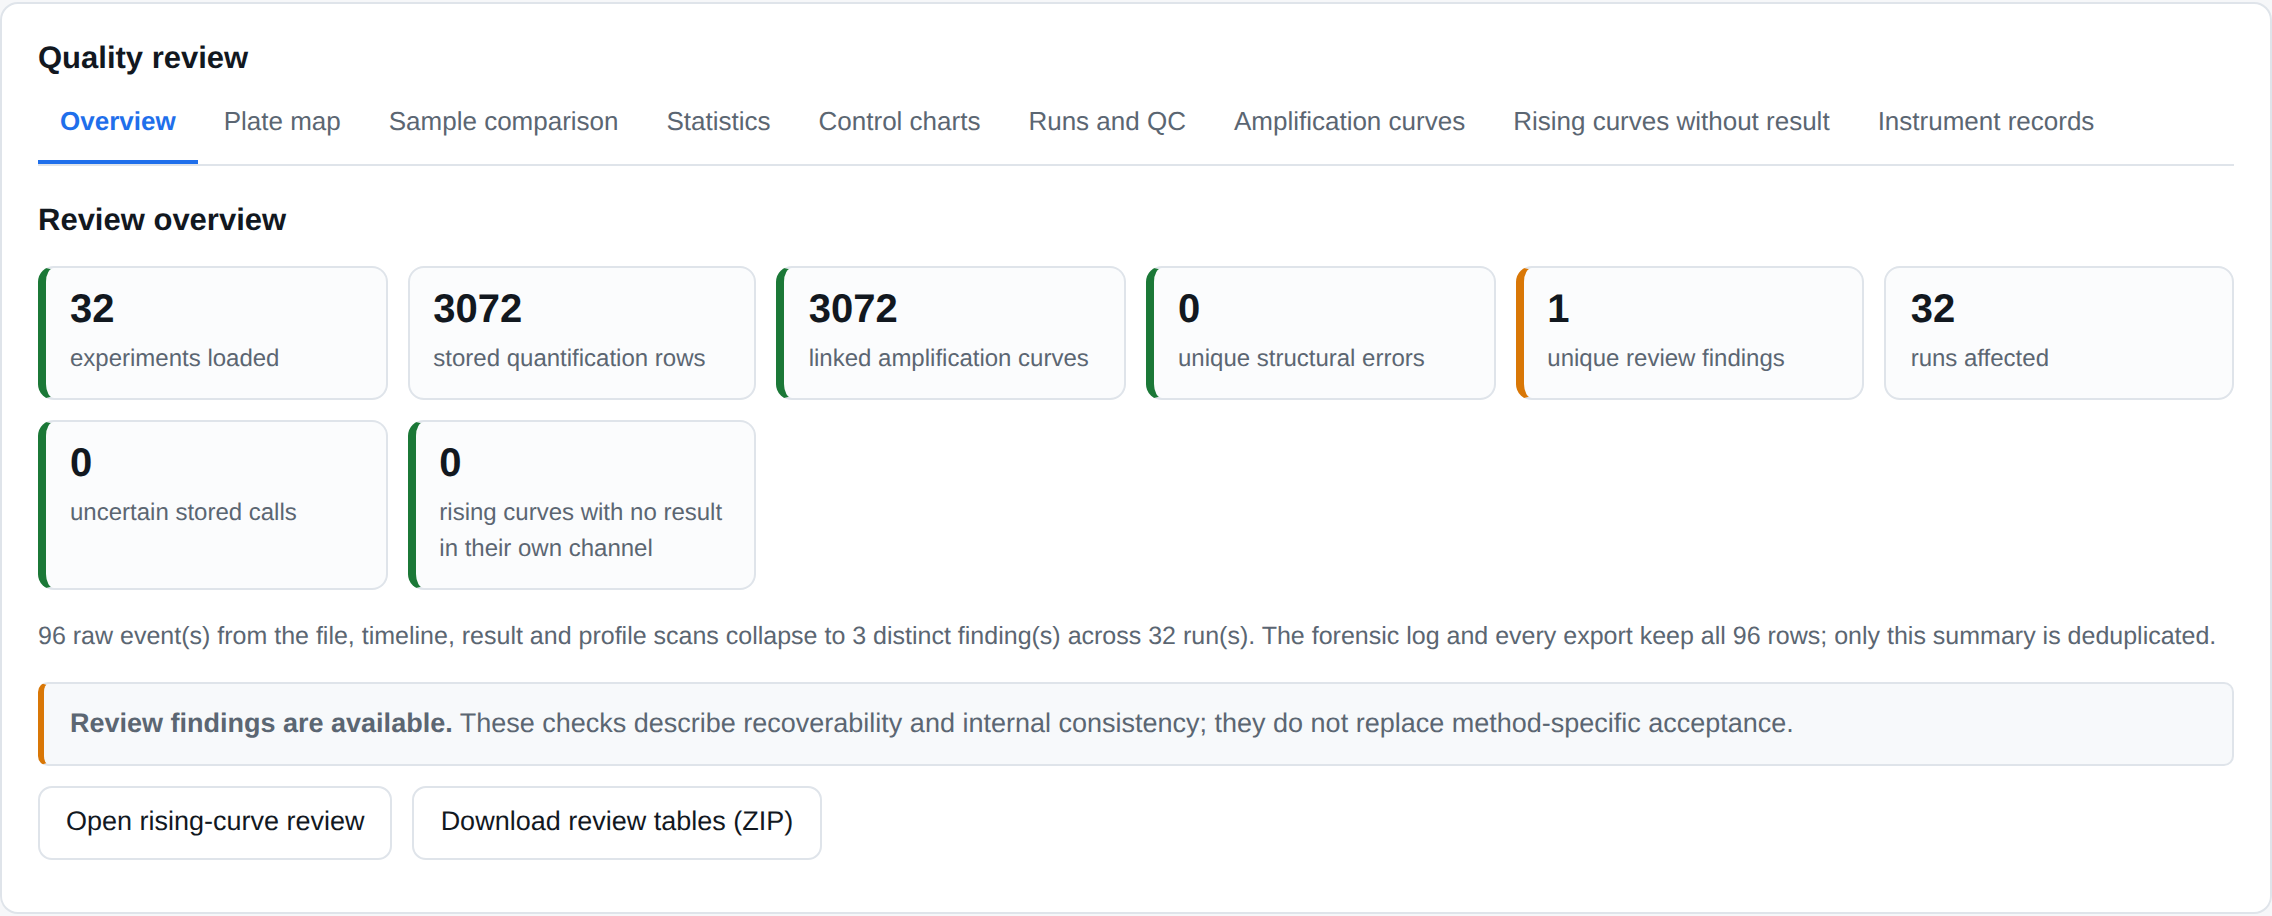
\includegraphics[width=0.96\linewidth,height=0.80\textheight,keepaspectratio]{fig/gallery/tab_review.png}
\caption[Quality and forensic review]{\synthtag Quality and forensic review. {\footnotesize Exercises \texttt{currentReviewSheet}, \texttt{renderReviewSheetLazy}, \texttt{reviewForensicEvents}, \texttt{reviewRunRows} and 231 more function(s) reachable from them.}}
\label{fig:gal-tab-review}
\end{figure}

\begin{figure}[H]\centering
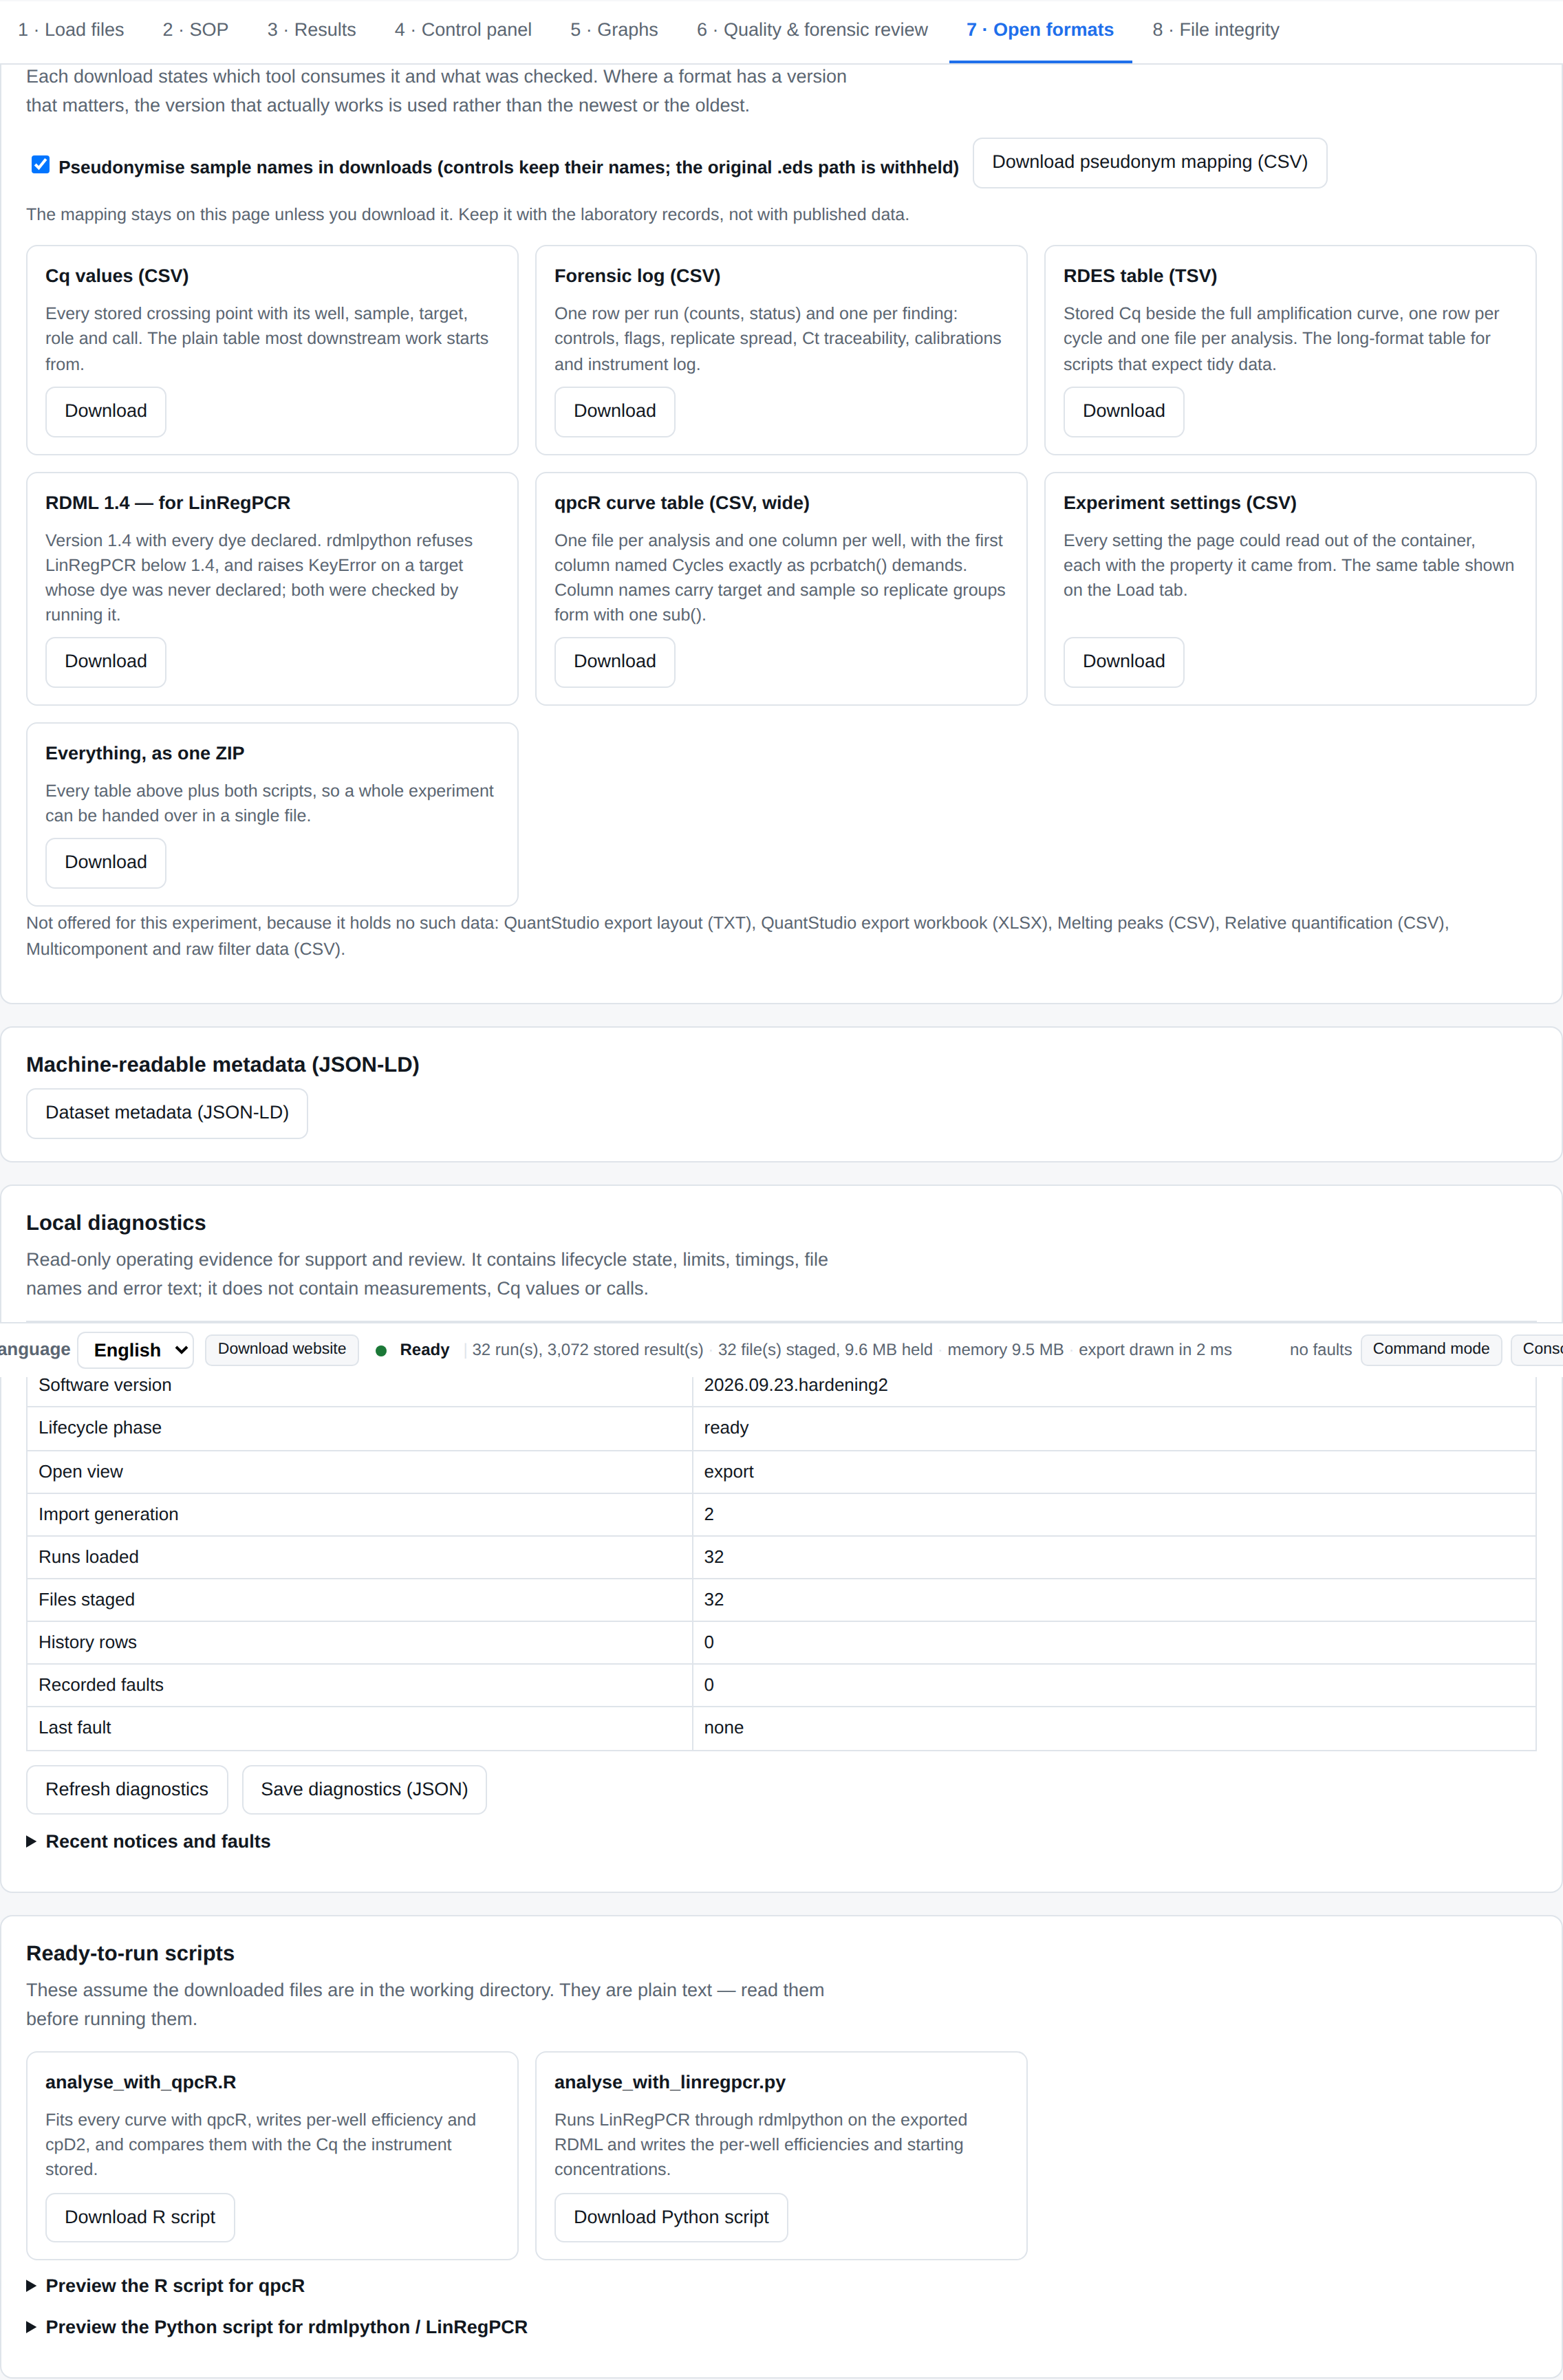
\includegraphics[width=0.96\linewidth,height=0.80\textheight,keepaspectratio]{fig/gallery/tab_export.png}
\caption[Open formats: what can be taken out]{\synthtag Open formats: what can be taken out. {\footnotesize Exercises \texttt{renderExports}, \texttt{selCatalogue}, \texttt{selDataItems}, \texttt{selImageItems} and 194 more function(s) reachable from them.}}
\label{fig:gal-tab-export}
\end{figure}

\begin{figure}[H]\centering
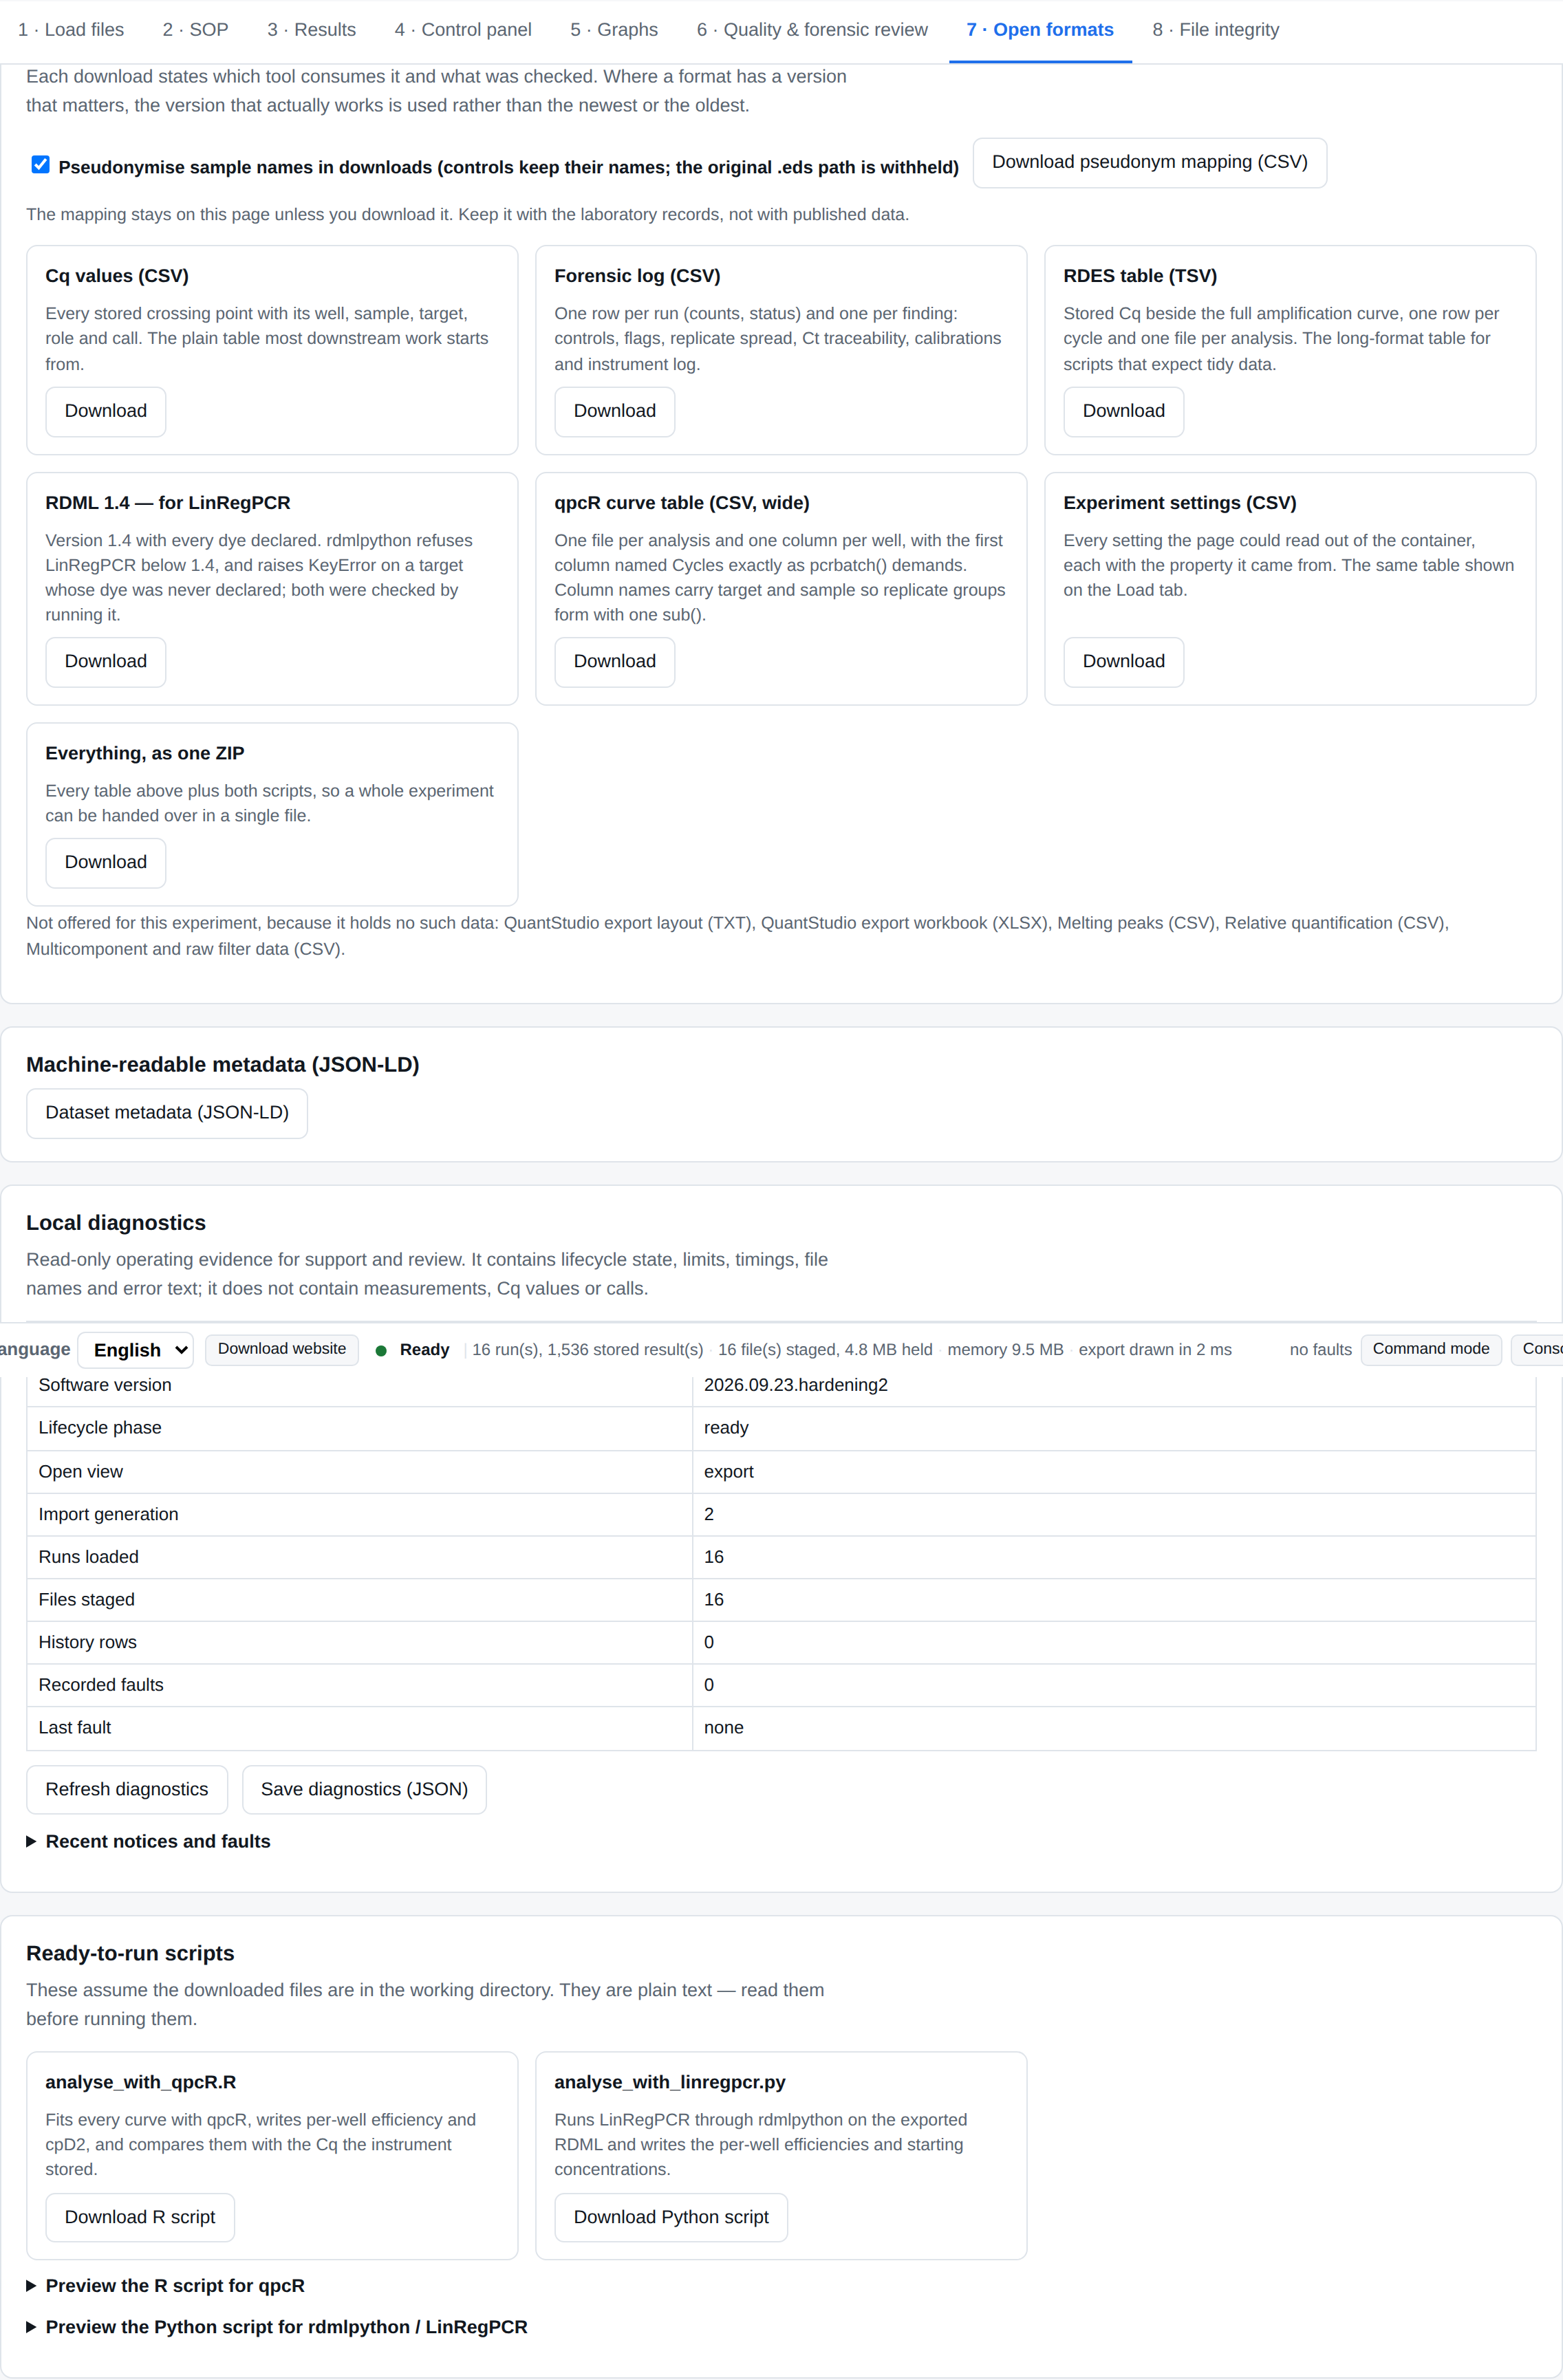
\includegraphics[width=0.96\linewidth,height=0.80\textheight,keepaspectratio]{fig/gallery/export_catalogue.png}
\caption[Open formats: the catalogue of everything that can leave the page]{\synthtag Open formats: the catalogue of everything that can leave the page. {\footnotesize Exercises \texttt{renderExports}, \texttt{selCatalogue}, \texttt{selChartItems}, \texttt{selDataItems}, \texttt{selImageItems}, \texttt{selZipEntries} and 201 more function(s) reachable from them.}}
\label{fig:gal-export-catalogue}
\end{figure}

\begin{figure}[H]\centering
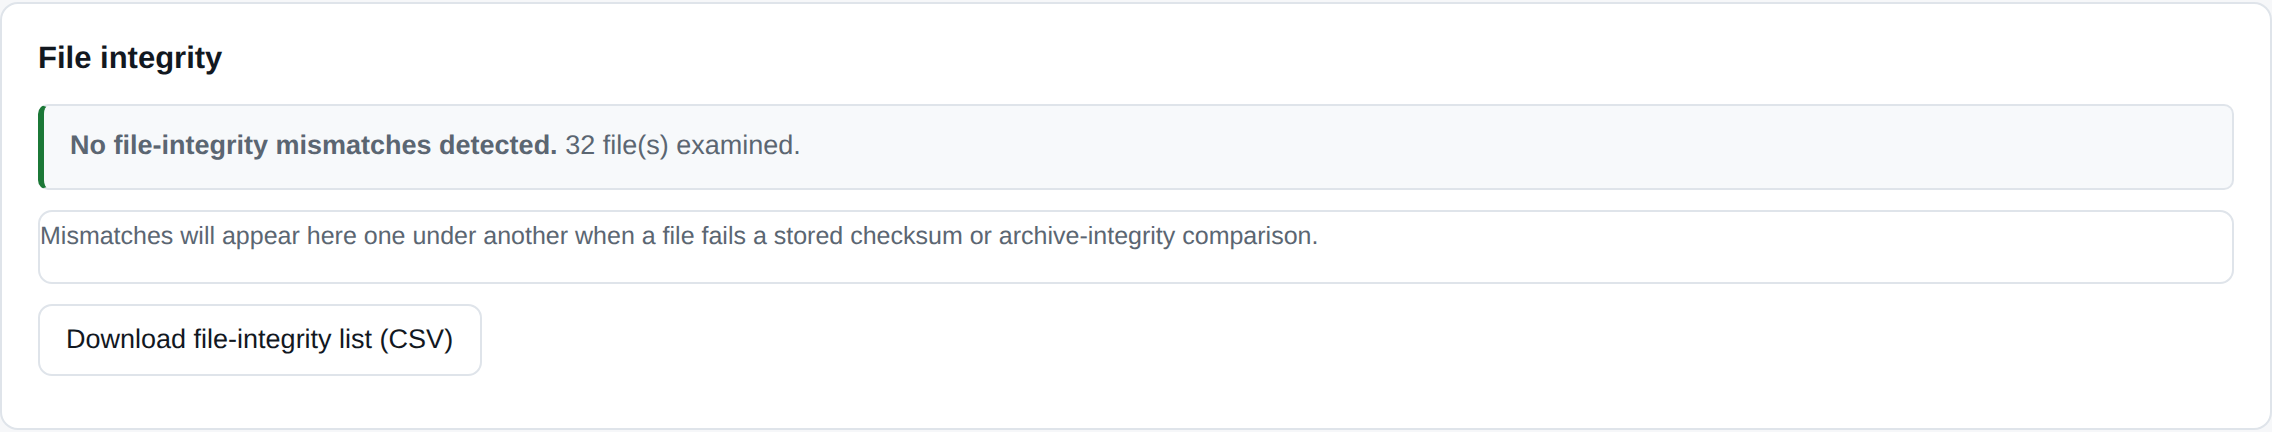
\includegraphics[width=0.96\linewidth,height=0.80\textheight,keepaspectratio]{fig/gallery/tab_integrity.png}
\caption[File integrity]{\synthtag File integrity. {\footnotesize Exercises \texttt{md5}, \texttt{renderIntegrity}, \texttt{sha256Hex} and 7 more function(s) reachable from them.}}
\label{fig:gal-tab-integrity}
\end{figure}

\section{The console and the two operator modes}
\begin{figure}[H]\centering
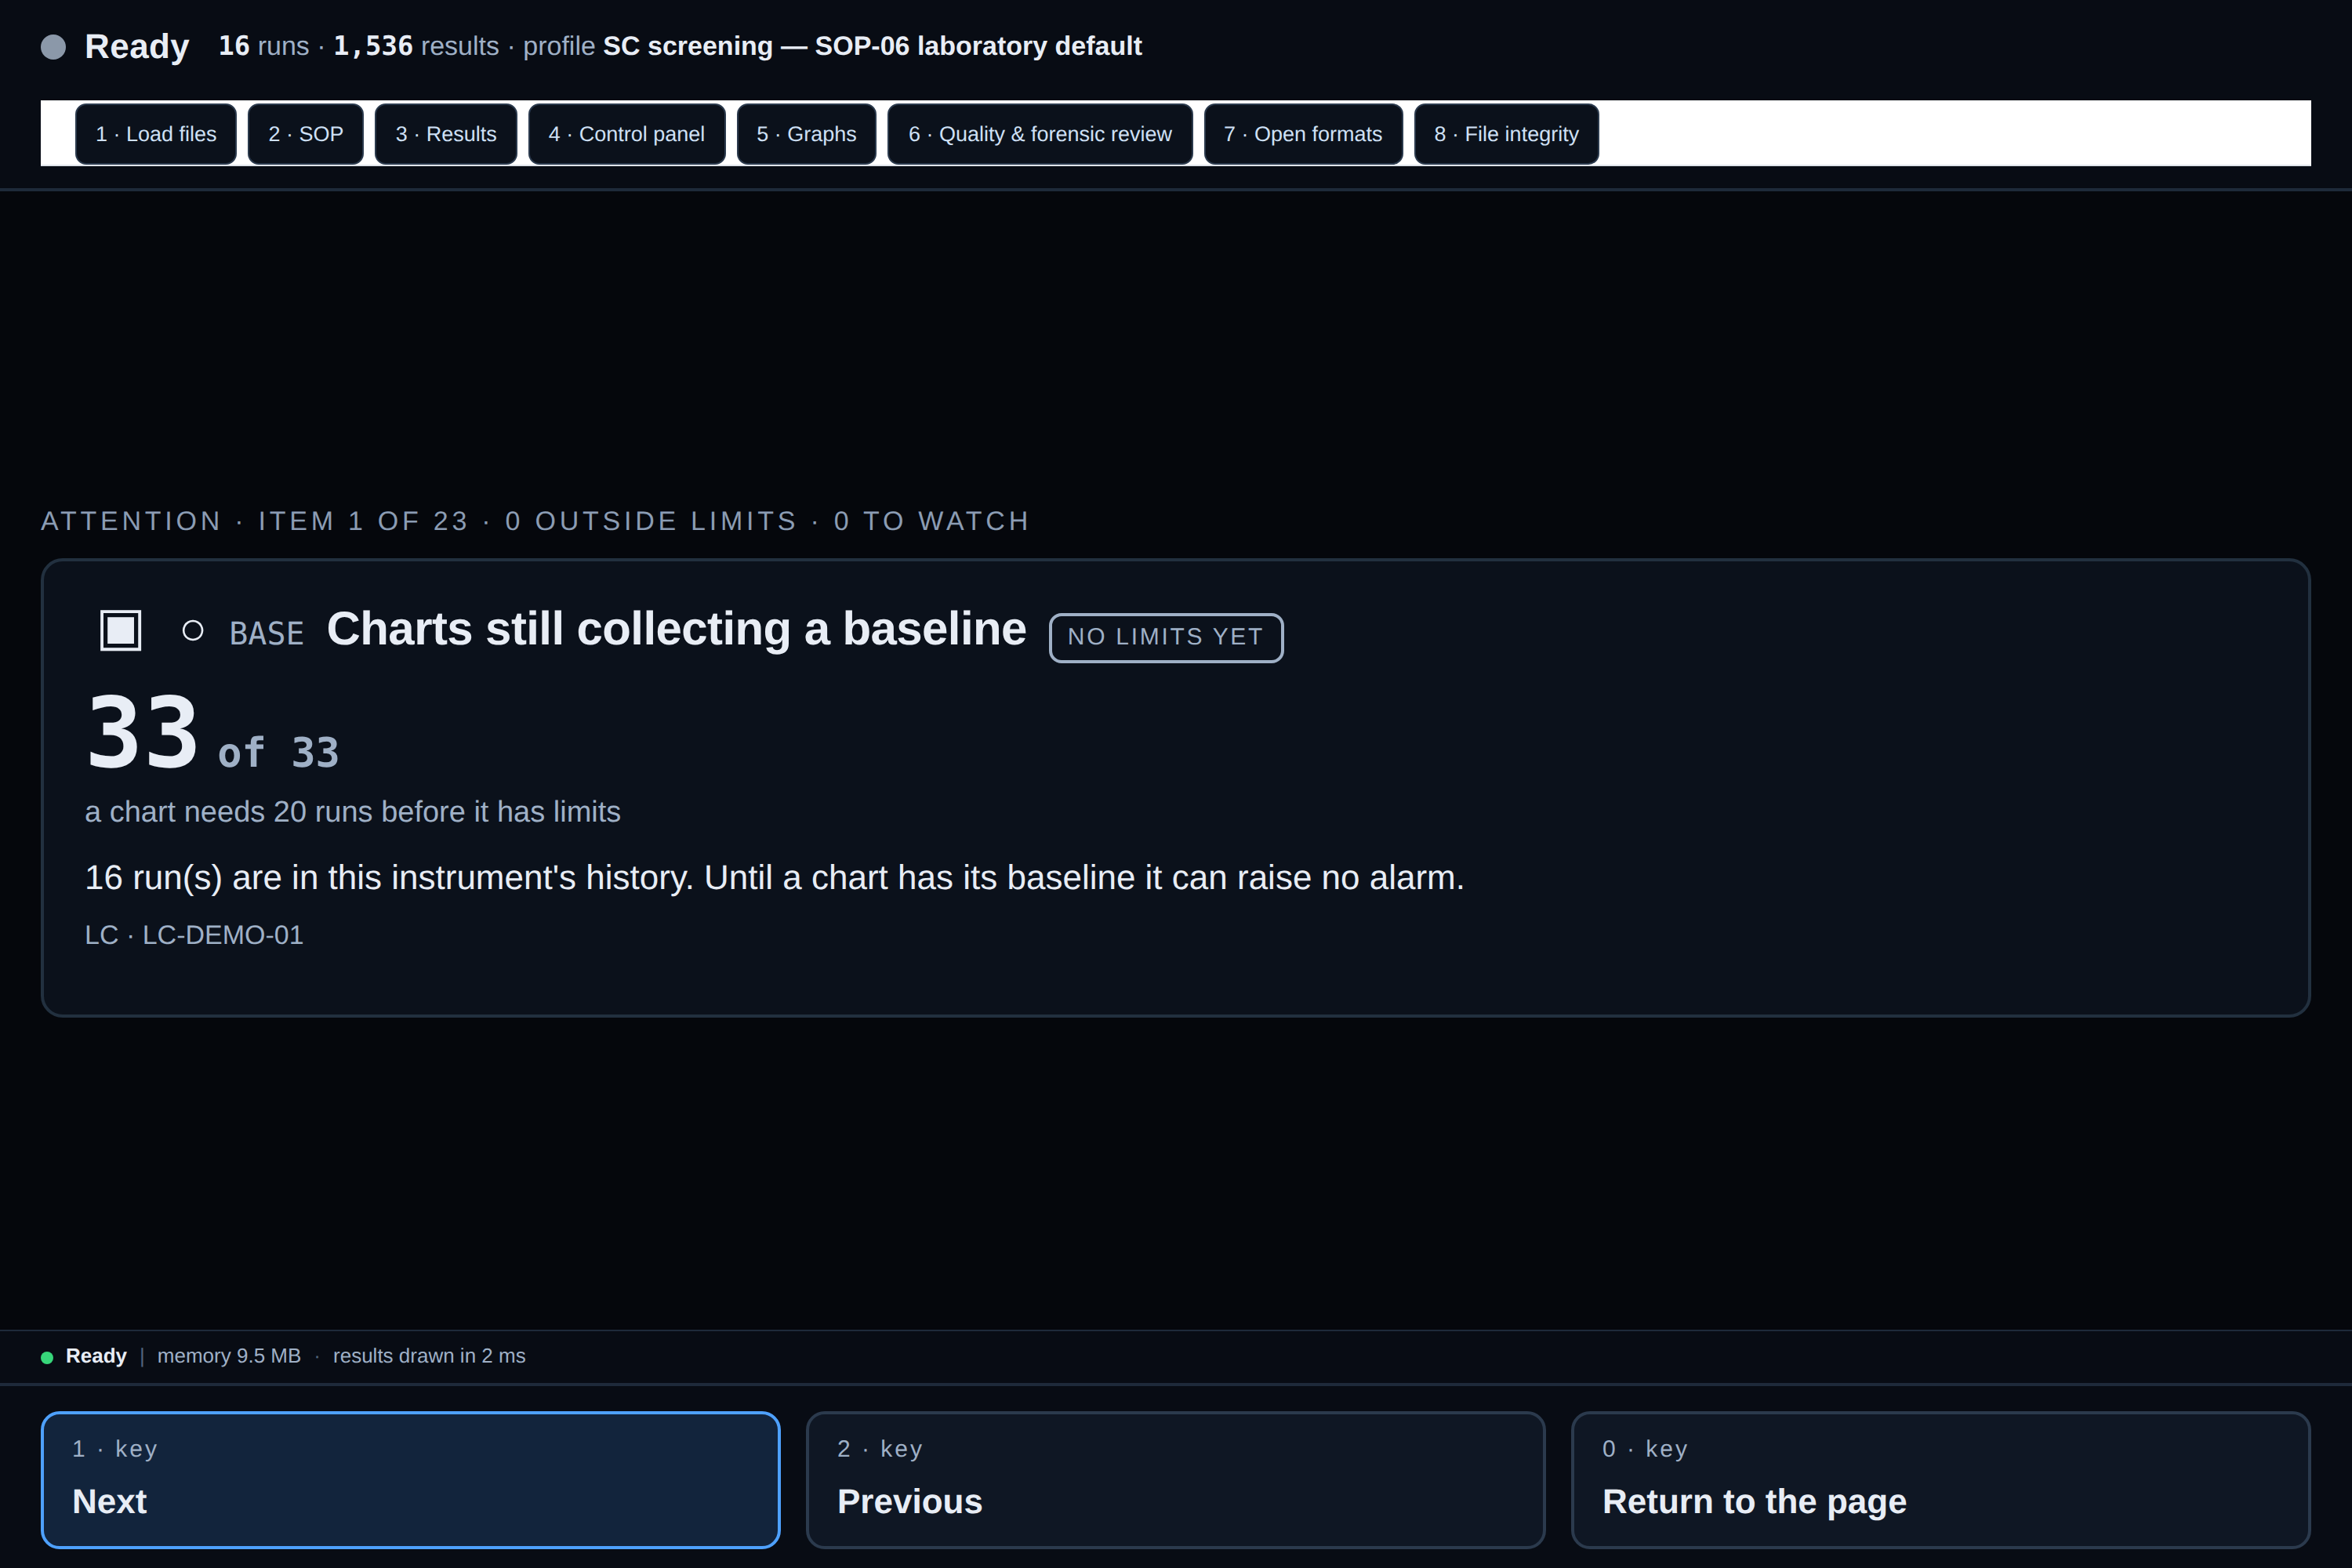
\includegraphics[width=0.96\linewidth,height=0.80\textheight,keepaspectratio]{fig/gallery/console.png}
\caption[The console: every finding as one item]{\synthtag The console: every finding as one item. {\footnotesize Exercises \texttt{mgIt}, \texttt{mgOpen}, \texttt{mgRender}, \texttt{mgViewLoad}, \texttt{mgViewSop} and 144 more function(s) reachable from them.}}
\label{fig:gal-console}
\end{figure}

\begin{figure}[H]\centering
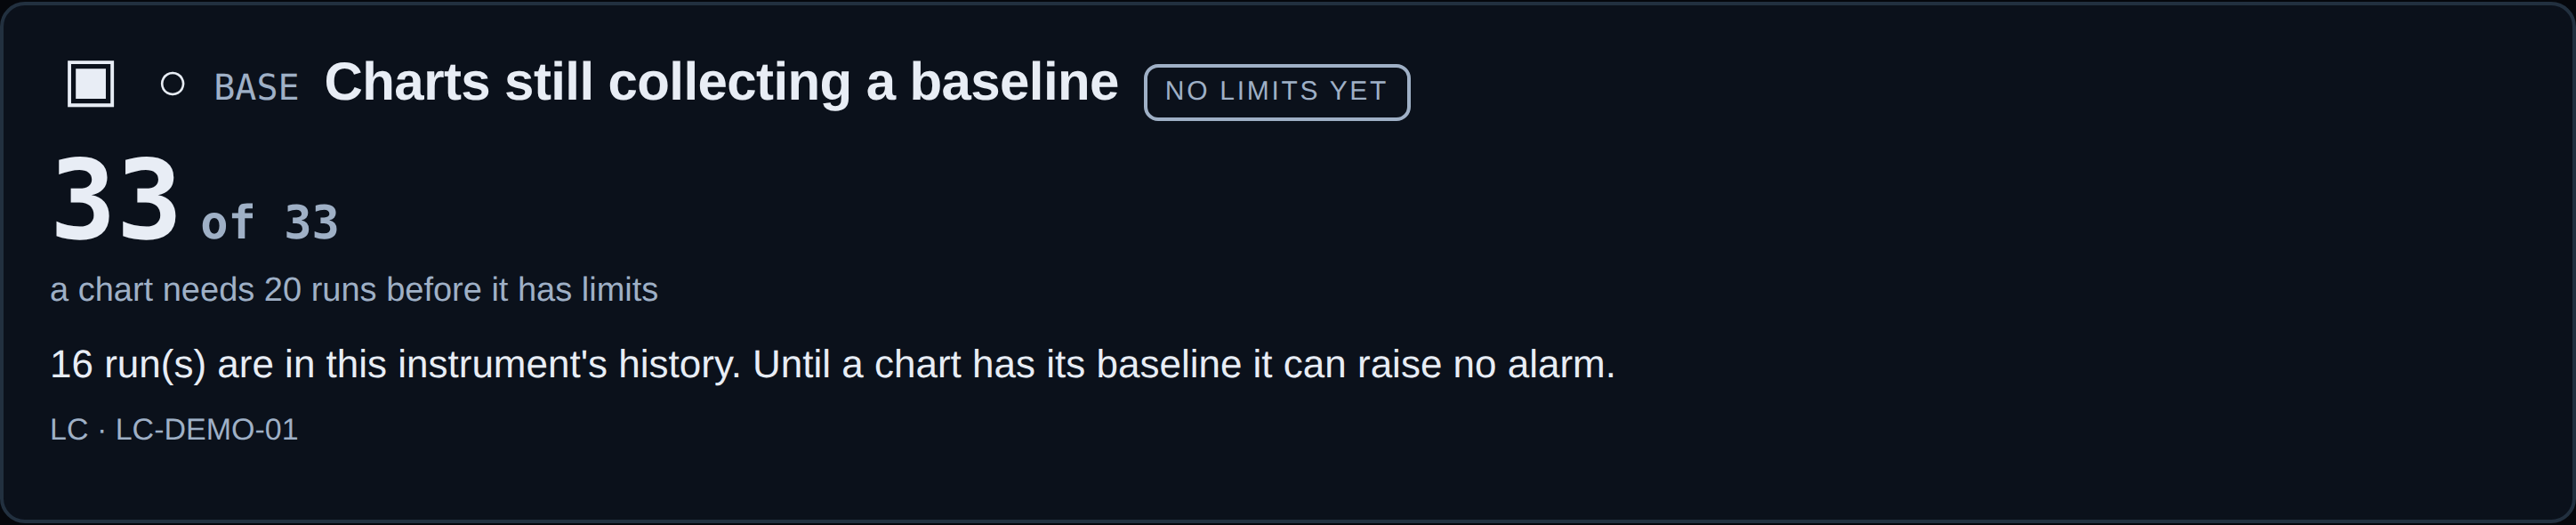
\includegraphics[width=0.96\linewidth,height=0.80\textheight,keepaspectratio]{fig/gallery/console_item.png}
\caption[One console item, with its evidence and actions]{\synthtag One console item, with its evidence and actions. {\footnotesize Exercises \texttt{mgRender} and 134 more function(s) reachable from them.}}
\label{fig:gal-console-item}
\end{figure}

\begin{figure}[H]\centering
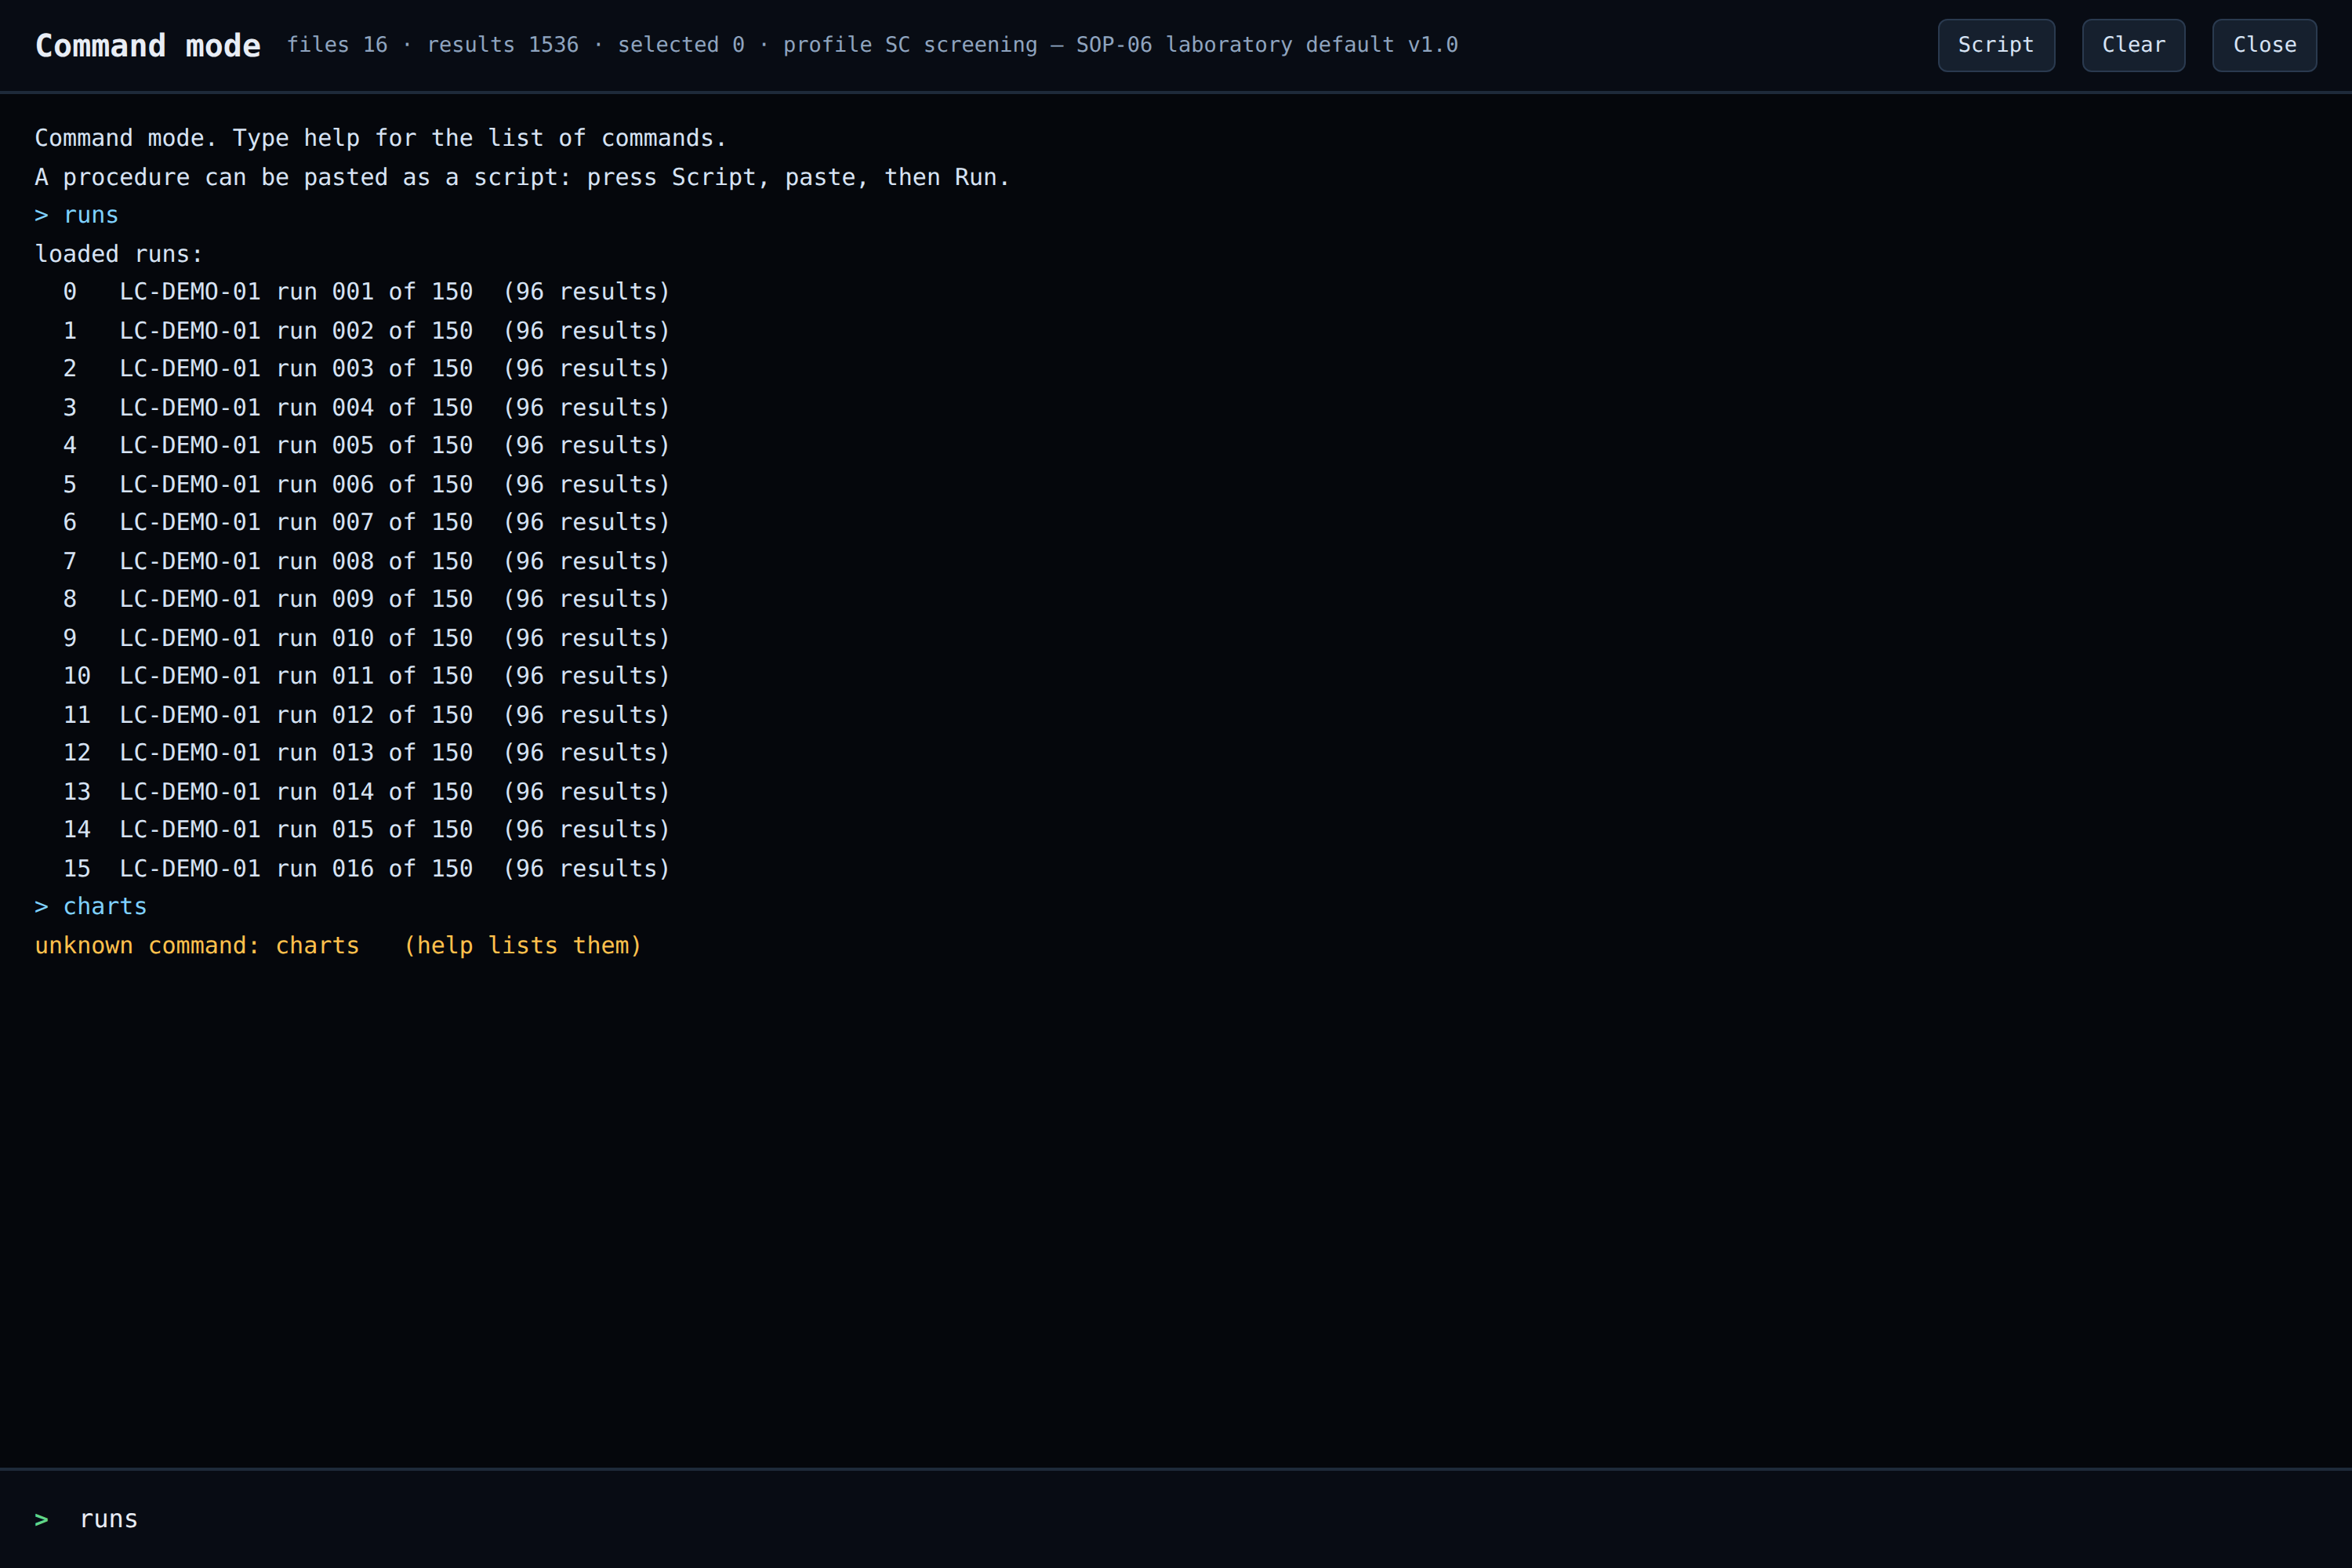
\includegraphics[width=0.96\linewidth,height=0.80\textheight,keepaspectratio]{fig/gallery/command_mode.png}
\caption[Command mode: the same catalogue as a command line]{\synthtag Command mode: the same catalogue as a command line. {\footnotesize Exercises \texttt{cmdExec}, \texttt{cmdOpen}, \texttt{cmdPrint}, \texttt{cmdRunLine}, \texttt{cmdTable} and 205 more function(s) reachable from them.}}
\label{fig:gal-command-mode}
\end{figure}

\begin{figure}[H]\centering
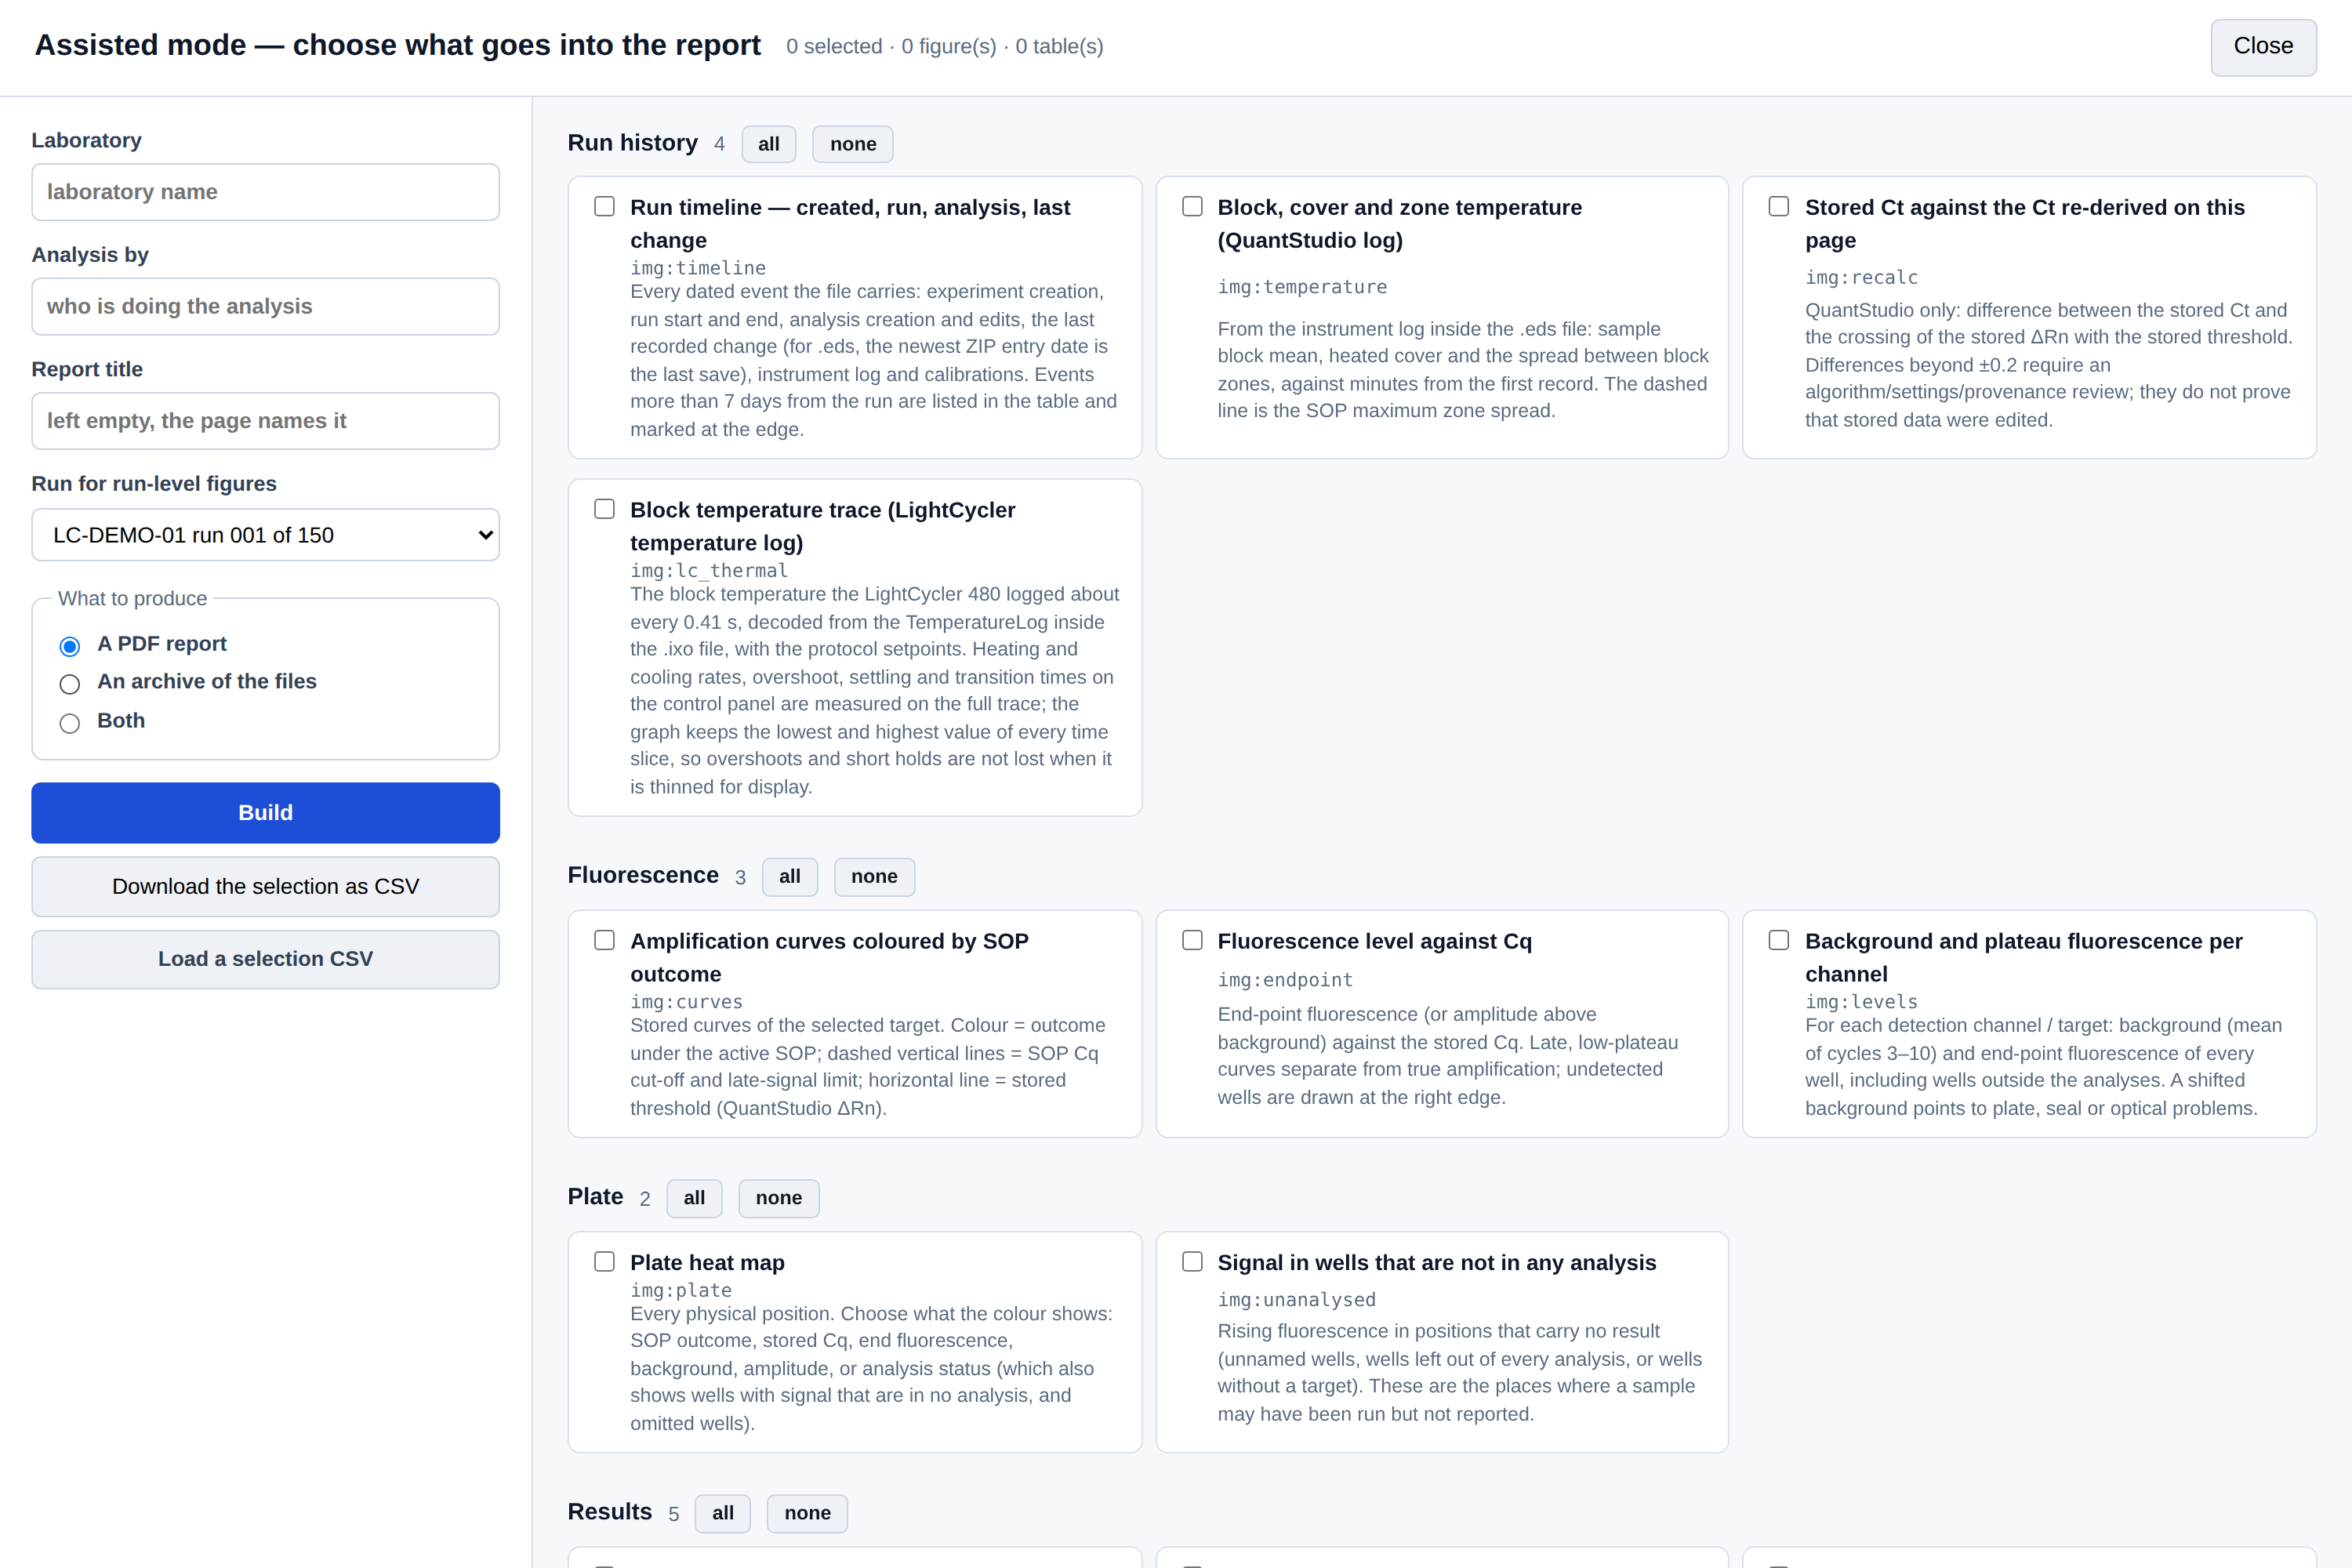
\includegraphics[width=0.96\linewidth,height=0.80\textheight,keepaspectratio]{fig/gallery/assisted_mode.png}
\caption[Assisted mode: the same catalogue as a guided selection]{\synthtag Assisted mode: the same catalogue as a guided selection. {\footnotesize Exercises \texttt{astBuild}, \texttt{astCount}, \texttt{astOpen}, \texttt{astOutput}, \texttt{astRender} and 170 more function(s) reachable from them.}}
\label{fig:gal-assisted-mode}
\end{figure}

\section{Graphs}\label{sec:gal-graphs}
All twenty-five graphs of the current build, in the order the page lists them. A view with no data in this demonstration set is shown as the page shows it, with its message.

\begin{figure}[H]\centering
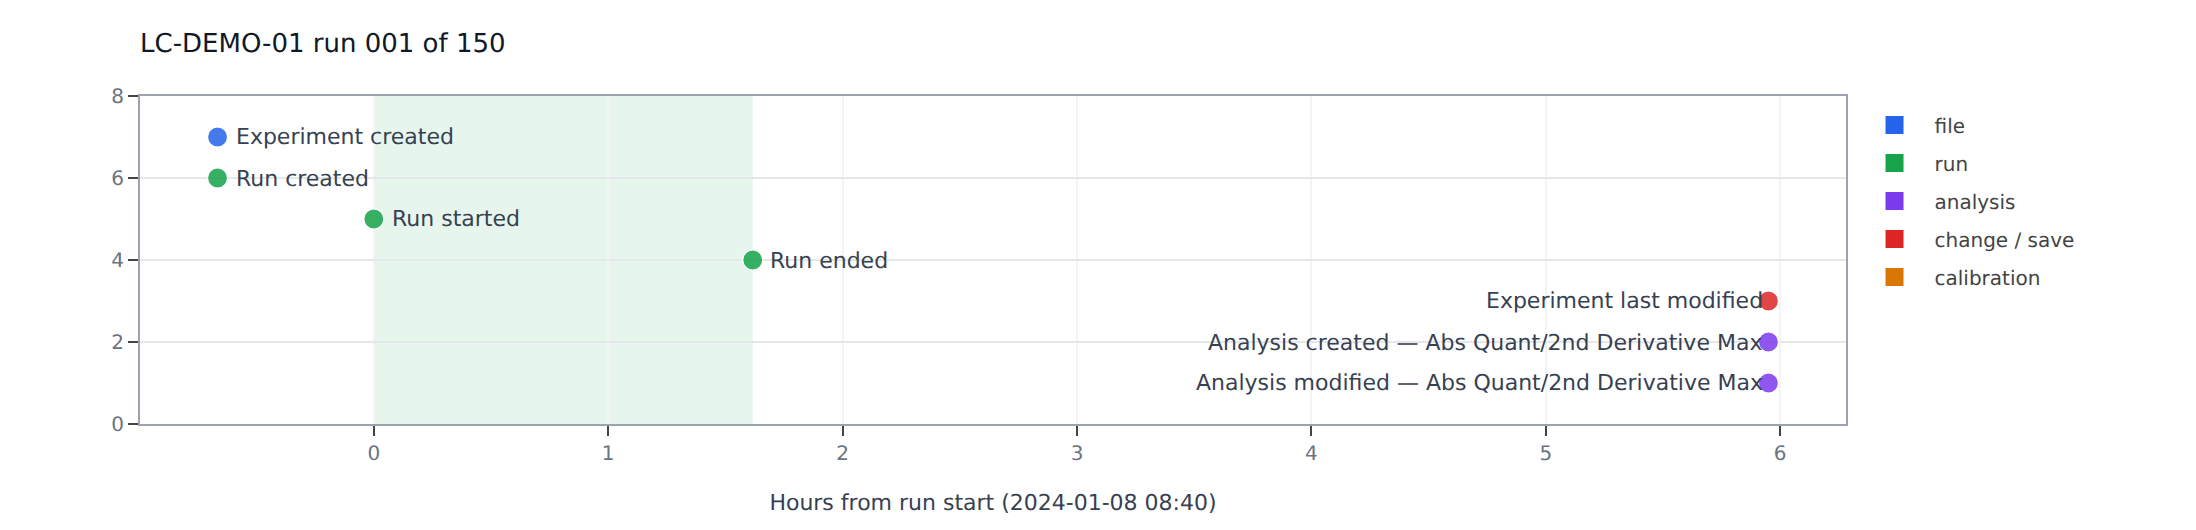
\includegraphics[width=0.92\linewidth,height=0.80\textheight,keepaspectratio]{fig/gallery/graph_timeline.png}
\caption[Run timeline — created, run, analysis, last change]{\synthtag Run timeline — created, run, analysis, last change. {\footnotesize Exercises \texttt{extent}, \texttt{gByDate}, \texttt{gCutLines}, \texttt{gRunTicks}, \texttt{gRunWells}, \texttt{gTargets} and 56 more function(s) reachable from them.}}
\label{fig:gal-graph-timeline}
\end{figure}

\begin{figure}[H]\centering
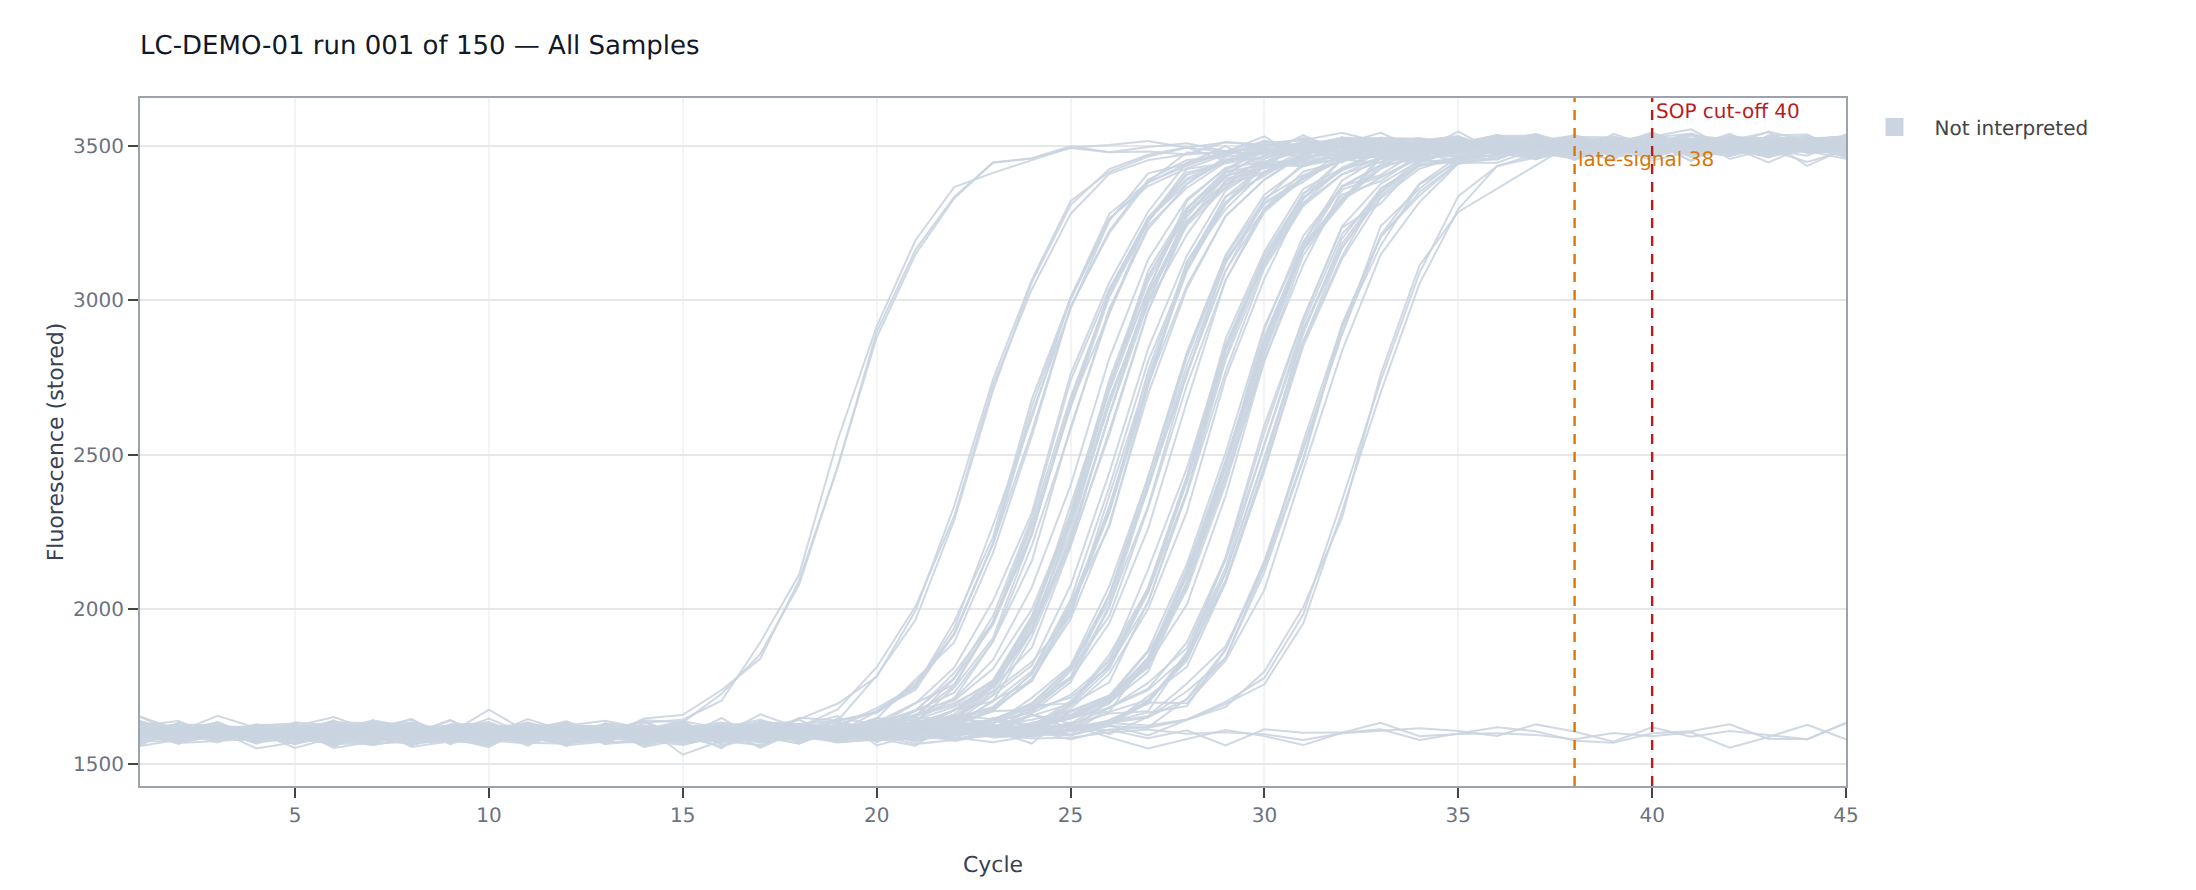
\includegraphics[width=0.92\linewidth,height=0.80\textheight,keepaspectratio]{fig/gallery/graph_curves.png}
\caption[Amplification curves coloured by SOP outcome]{\synthtag Amplification curves coloured by SOP outcome. {\footnotesize Exercises \texttt{extent}, \texttt{gByDate}, \texttt{gCutLines}, \texttt{gRunTicks}, \texttt{gRunWells}, \texttt{gTargets} and 56 more function(s) reachable from them.}}
\label{fig:gal-graph-curves}
\end{figure}

\begin{figure}[H]\centering
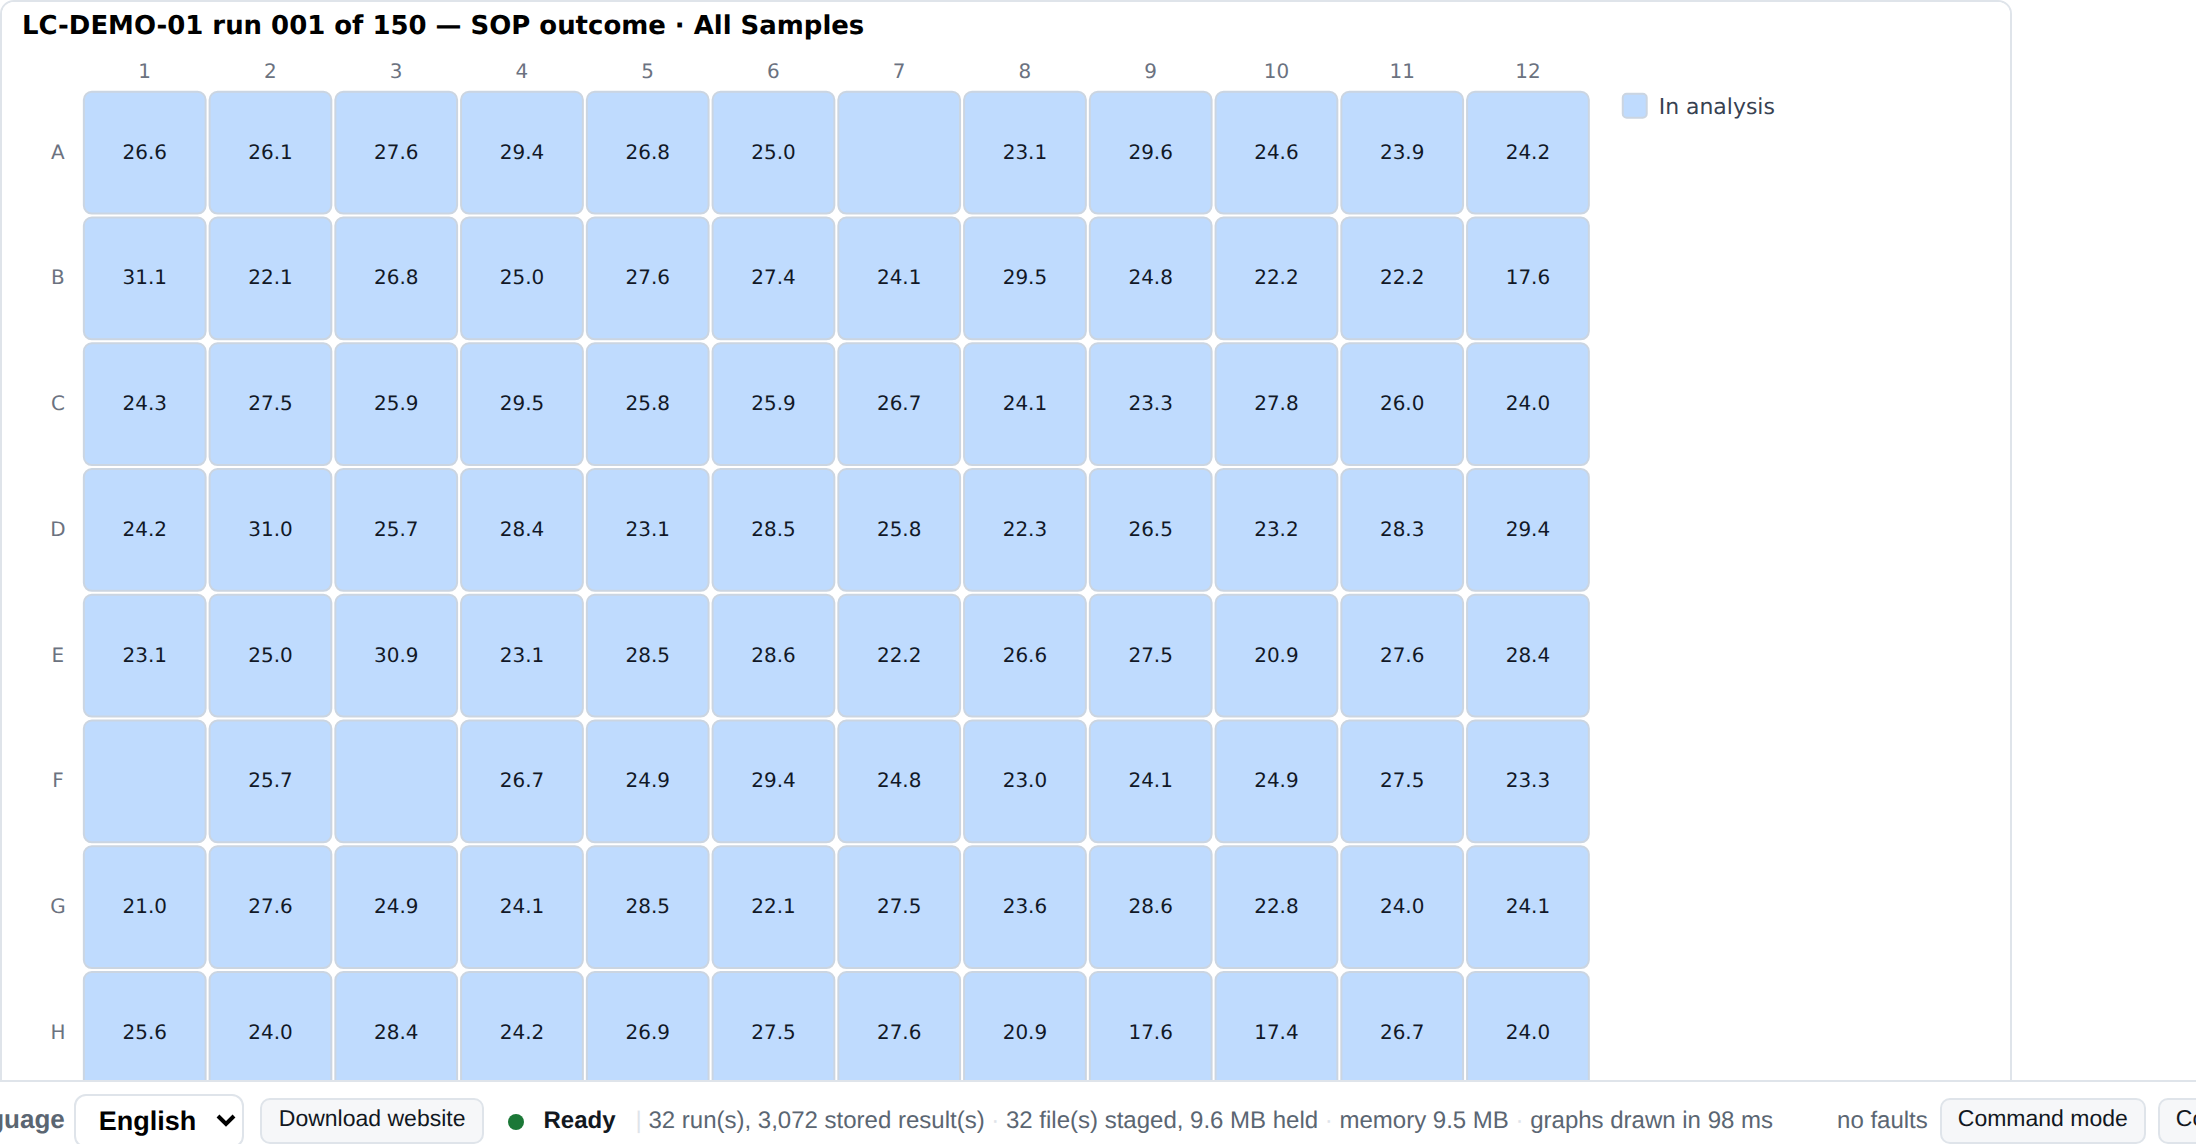
\includegraphics[width=0.92\linewidth,height=0.80\textheight,keepaspectratio]{fig/gallery/graph_plate.png}
\caption[Plate heat map]{\synthtag Plate heat map. {\footnotesize Exercises \texttt{extent}, \texttt{gByDate}, \texttt{gCutLines}, \texttt{gRunTicks}, \texttt{gRunWells}, \texttt{gTargets} and 56 more function(s) reachable from them.}}
\label{fig:gal-graph-plate}
\end{figure}

\begin{figure}[H]\centering

\includegraphics[width=0.92\linewidth,height=0.80\textheight,keepaspectratio]{fig/gallery/graph_unanalysed.png}
\caption[Signal in wells that are not in any analysis --- no data for this view in the demonstration set]{\synthtag Signal in wells that are not in any analysis --- no data for this view in the demonstration set. {\footnotesize Exercises \texttt{extent}, \texttt{gByDate}, \texttt{gCutLines}, \texttt{gRunTicks}, \texttt{gRunWells}, \texttt{gTargets} and 56 more function(s) reachable from them.}}
\label{fig:gal-graph-unanalysed}
\end{figure}

\begin{figure}[H]\centering
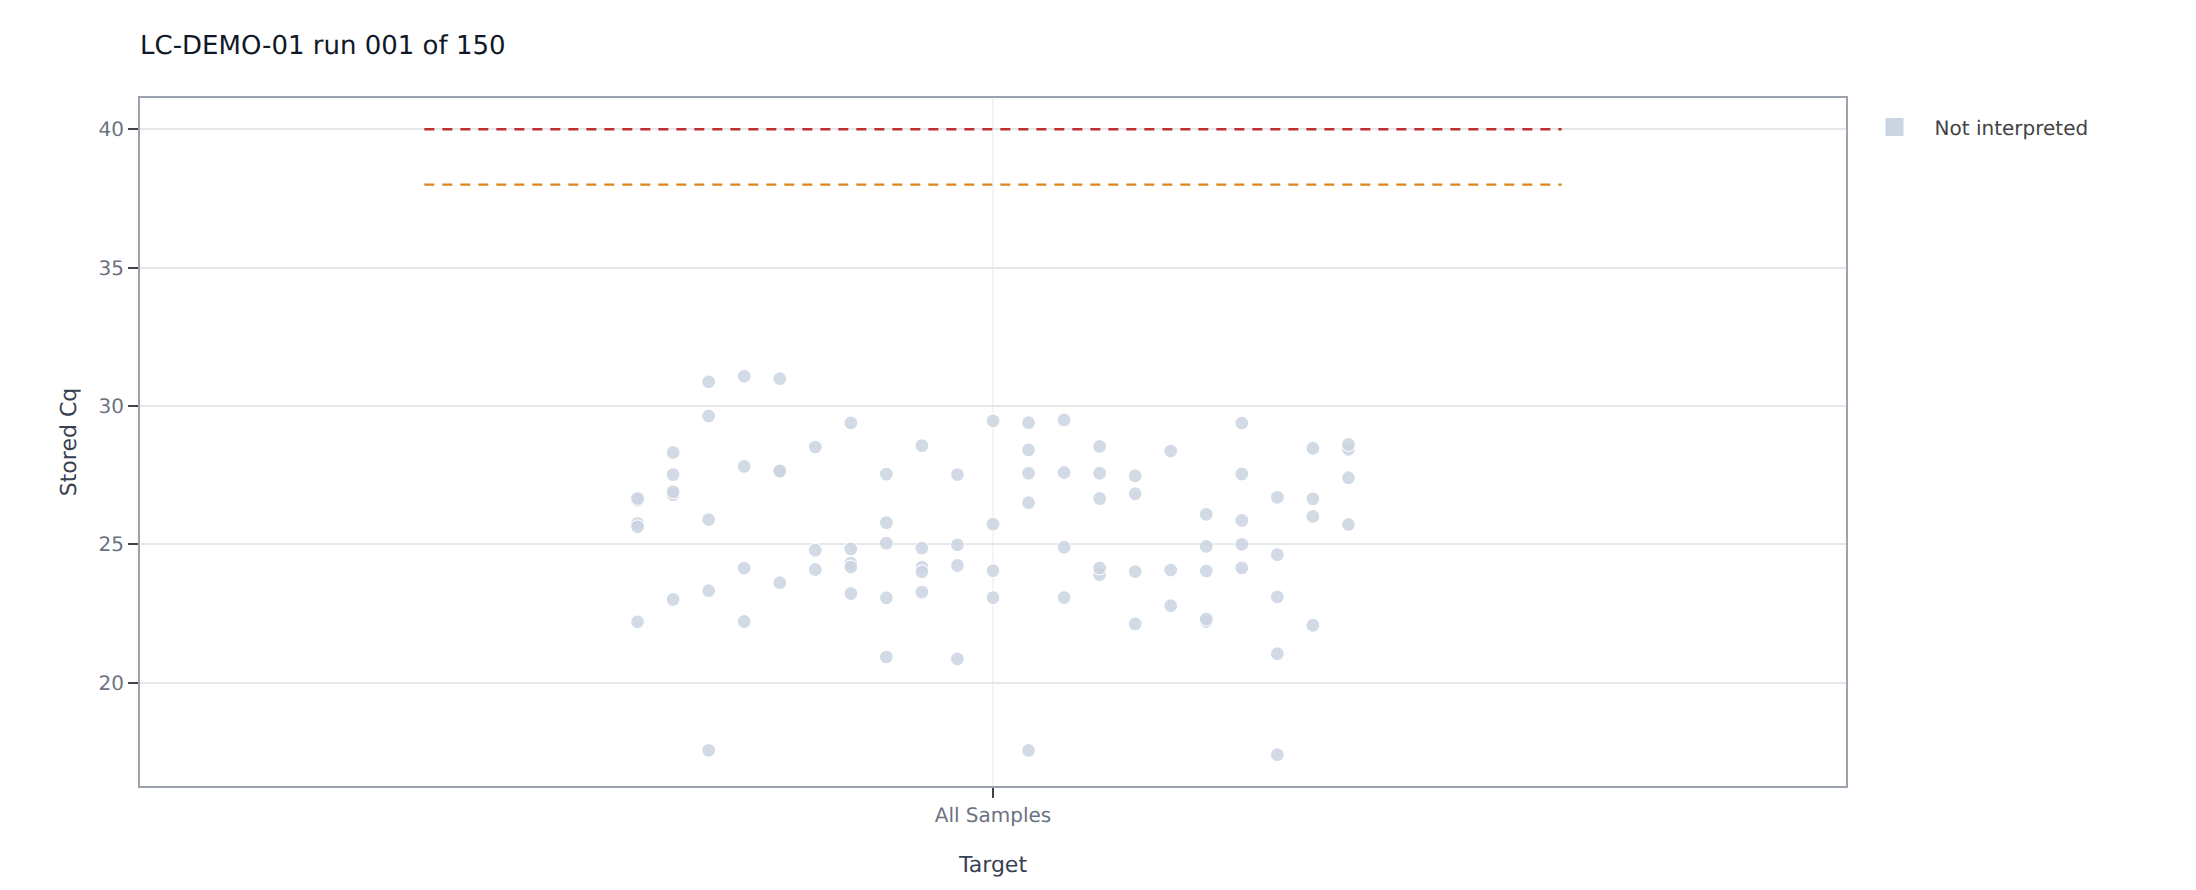
\includegraphics[width=0.92\linewidth,height=0.80\textheight,keepaspectratio]{fig/gallery/graph_cqstrip.png}
\caption[Cq by target with SOP cut-offs]{\synthtag Cq by target with SOP cut-offs. {\footnotesize Exercises \texttt{extent}, \texttt{gByDate}, \texttt{gCutLines}, \texttt{gRunTicks}, \texttt{gRunWells}, \texttt{gTargets} and 56 more function(s) reachable from them.}}
\label{fig:gal-graph-cqstrip}
\end{figure}

\begin{figure}[H]\centering
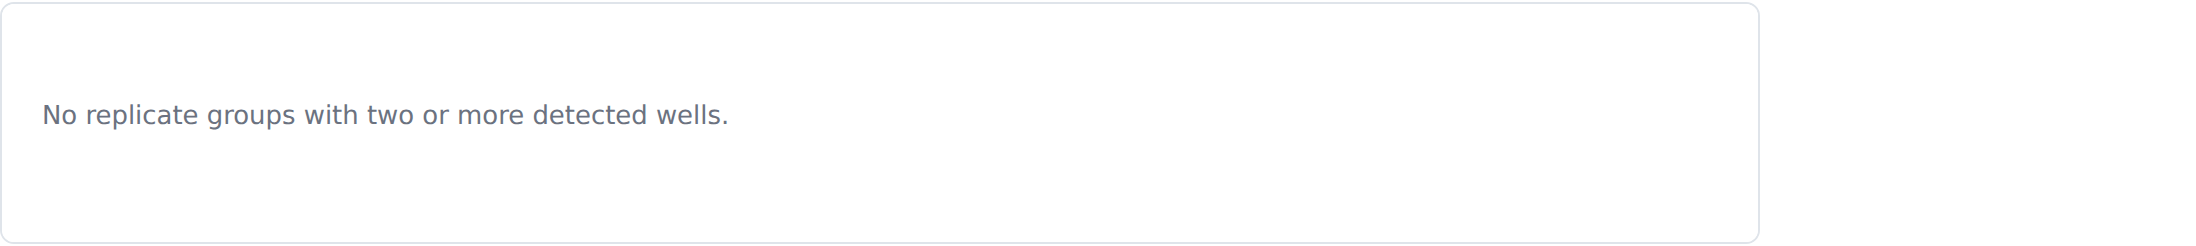
\includegraphics[width=0.92\linewidth,height=0.80\textheight,keepaspectratio]{fig/gallery/graph_repsd.png}
\caption[Replicate spread — mean Cq against SD --- no data for this view in the demonstration set]{\synthtag Replicate spread — mean Cq against SD --- no data for this view in the demonstration set. {\footnotesize Exercises \texttt{extent}, \texttt{gByDate}, \texttt{gCutLines}, \texttt{gRunTicks}, \texttt{gRunWells}, \texttt{gTargets} and 56 more function(s) reachable from them.}}
\label{fig:gal-graph-repsd}
\end{figure}

\begin{figure}[H]\centering
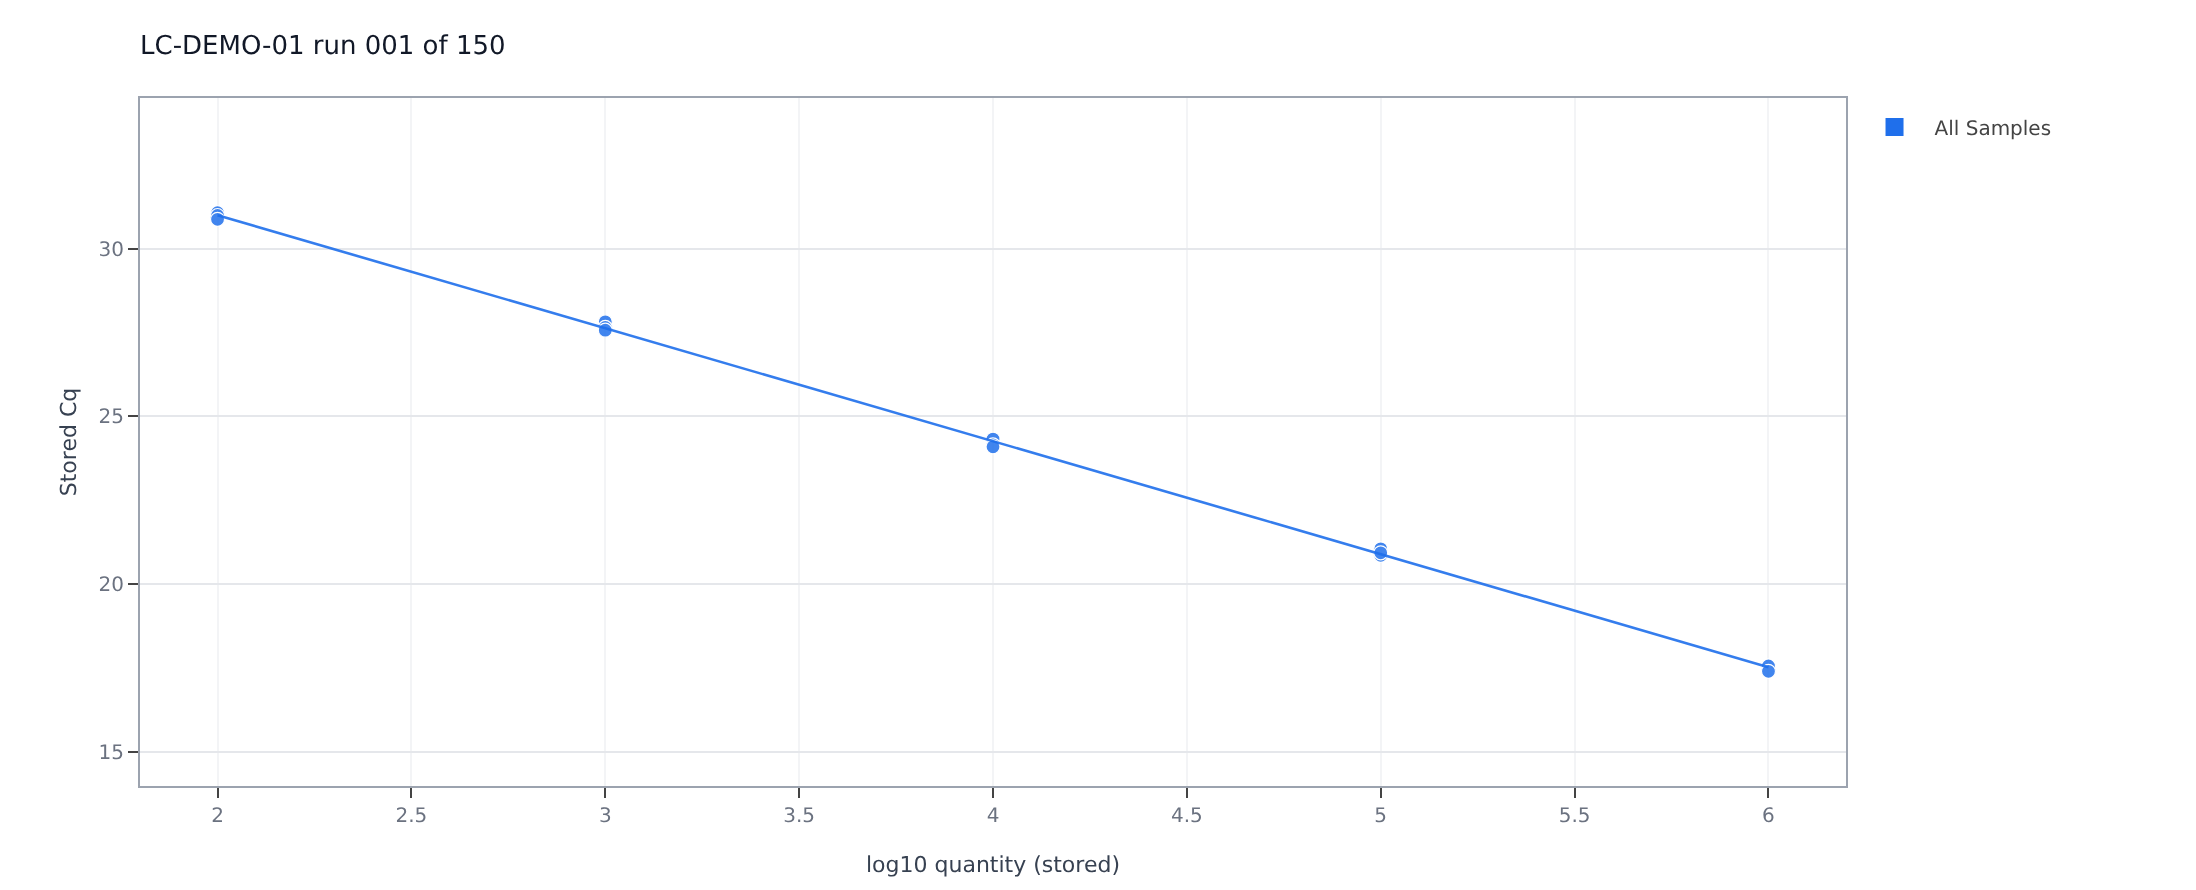
\includegraphics[width=0.92\linewidth,height=0.80\textheight,keepaspectratio]{fig/gallery/graph_stdcurve.png}
\caption[Standard curve with residuals and SOP limits]{\synthtag Standard curve with residuals and SOP limits. {\footnotesize Exercises \texttt{extent}, \texttt{gByDate}, \texttt{gCutLines}, \texttt{gRunTicks}, \texttt{gRunWells}, \texttt{gTargets} and 56 more function(s) reachable from them.}}
\label{fig:gal-graph-stdcurve}
\end{figure}

\begin{figure}[H]\centering

\includegraphics[width=0.92\linewidth,height=0.80\textheight,keepaspectratio]{fig/gallery/graph_ic.png}
\caption[Internal control / reference Cq per sample (inhibition) --- no data for this view in the demonstration set]{\synthtag Internal control / reference Cq per sample (inhibition) --- no data for this view in the demonstration set. {\footnotesize Exercises \texttt{extent}, \texttt{gByDate}, \texttt{gCutLines}, \texttt{gRunTicks}, \texttt{gRunWells}, \texttt{gTargets} and 56 more function(s) reachable from them.}}
\label{fig:gal-graph-ic}
\end{figure}

\begin{figure}[H]\centering
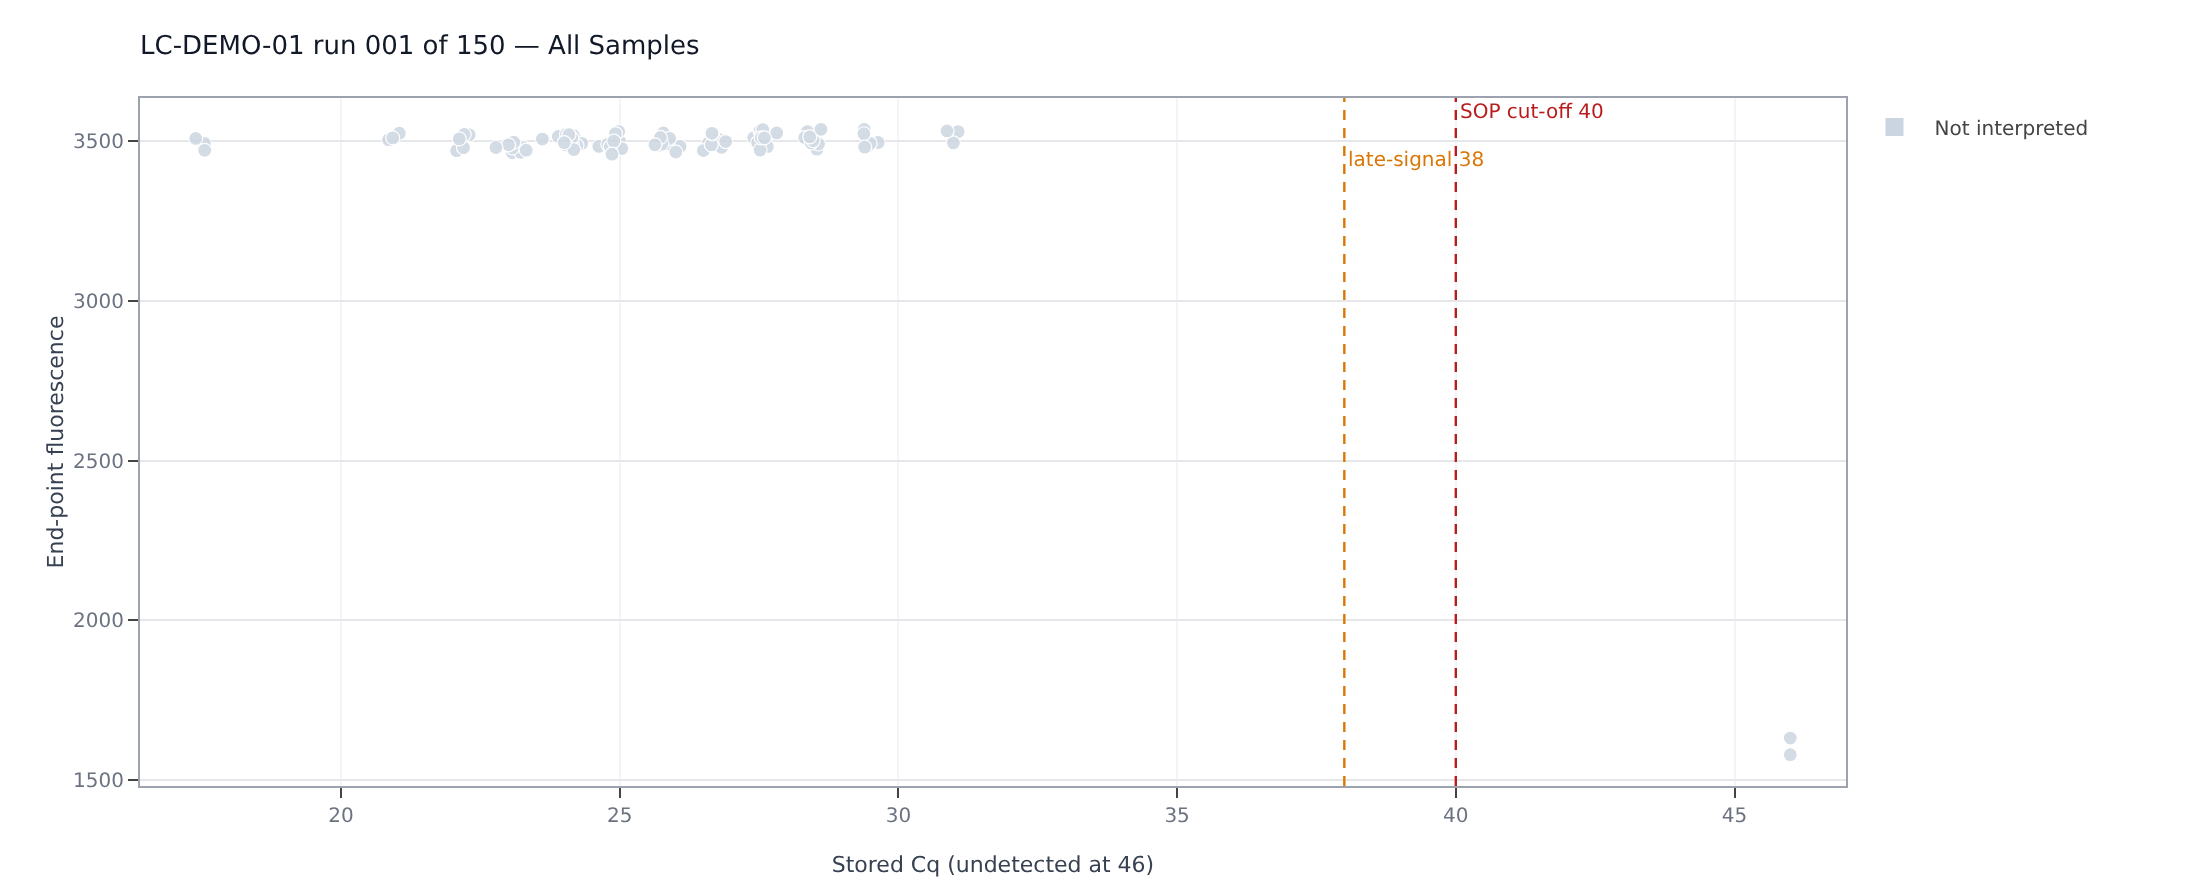
\includegraphics[width=0.92\linewidth,height=0.80\textheight,keepaspectratio]{fig/gallery/graph_endpoint.png}
\caption[Fluorescence level against Cq]{\synthtag Fluorescence level against Cq. {\footnotesize Exercises \texttt{extent}, \texttt{gByDate}, \texttt{gCutLines}, \texttt{gRunTicks}, \texttt{gRunWells}, \texttt{gTargets} and 56 more function(s) reachable from them.}}
\label{fig:gal-graph-endpoint}
\end{figure}

\begin{figure}[H]\centering
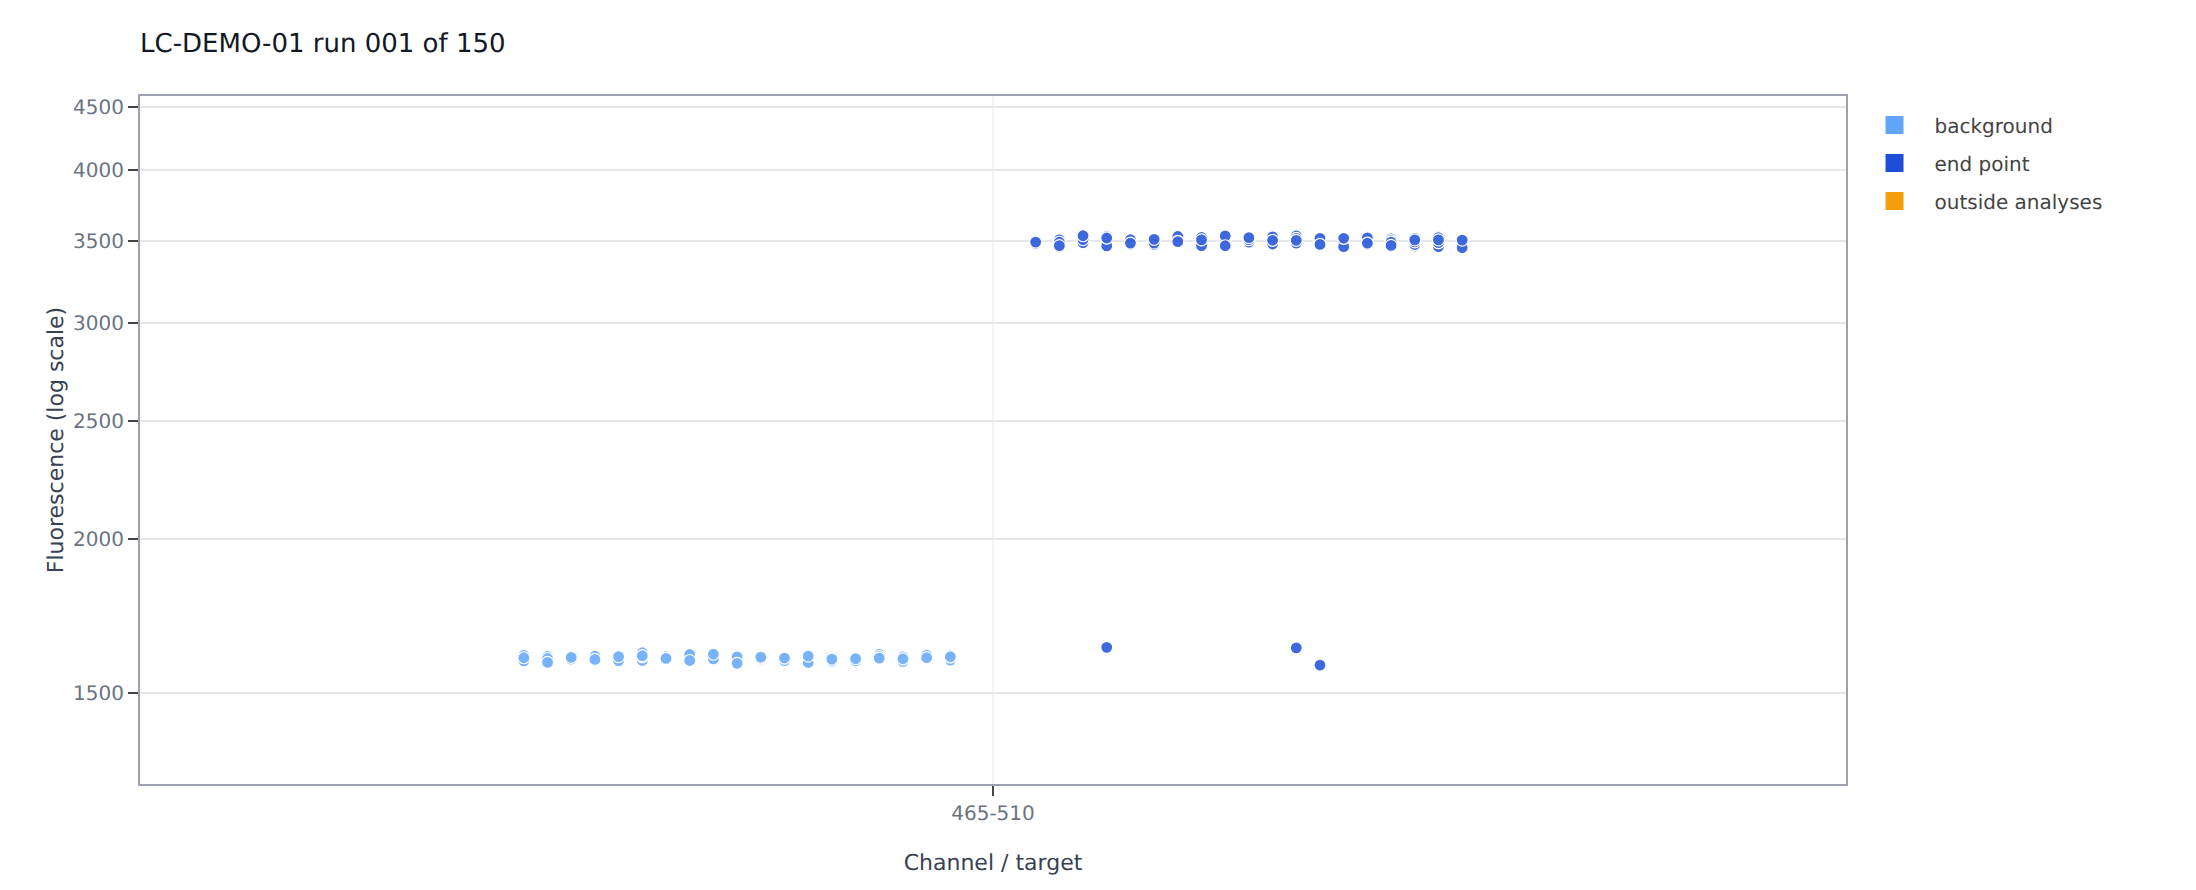
\includegraphics[width=0.92\linewidth,height=0.80\textheight,keepaspectratio]{fig/gallery/graph_levels.png}
\caption[Background and plateau fluorescence per channel]{\synthtag Background and plateau fluorescence per channel. {\footnotesize Exercises \texttt{extent}, \texttt{gByDate}, \texttt{gCutLines}, \texttt{gRunTicks}, \texttt{gRunWells}, \texttt{gTargets} and 56 more function(s) reachable from them.}}
\label{fig:gal-graph-levels}
\end{figure}

\begin{figure}[H]\centering

\includegraphics[width=0.92\linewidth,height=0.80\textheight,keepaspectratio]{fig/gallery/graph_outcomes.png}
\caption[SOP outcomes per target --- no data for this view in the demonstration set]{\synthtag SOP outcomes per target --- no data for this view in the demonstration set. {\footnotesize Exercises \texttt{extent}, \texttt{gByDate}, \texttt{gCutLines}, \texttt{gRunTicks}, \texttt{gRunWells}, \texttt{gTargets} and 56 more function(s) reachable from them.}}
\label{fig:gal-graph-outcomes}
\end{figure}

\begin{figure}[H]\centering
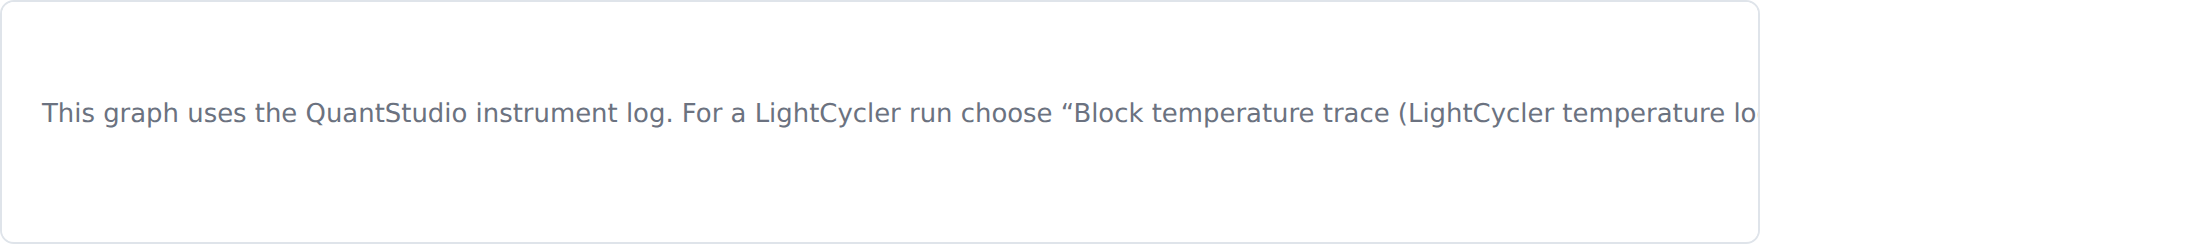
\includegraphics[width=0.92\linewidth,height=0.80\textheight,keepaspectratio]{fig/gallery/graph_temperature.png}
\caption[Block, cover and zone temperature (QuantStudio log) --- no data for this view in the demonstration set]{\synthtag Block, cover and zone temperature (QuantStudio log) --- no data for this view in the demonstration set. {\footnotesize Exercises \texttt{extent}, \texttt{gByDate}, \texttt{gCutLines}, \texttt{gRunTicks}, \texttt{gRunWells}, \texttt{gTargets} and 56 more function(s) reachable from them.}}
\label{fig:gal-graph-temperature}
\end{figure}

\begin{figure}[H]\centering

\includegraphics[width=0.92\linewidth,height=0.80\textheight,keepaspectratio]{fig/gallery/graph_recalc.png}
\caption[Stored Ct against the Ct re-derived on this page --- no data for this view in the demonstration set]{\synthtag Stored Ct against the Ct re-derived on this page --- no data for this view in the demonstration set. {\footnotesize Exercises \texttt{extent}, \texttt{gByDate}, \texttt{gCutLines}, \texttt{gRunTicks}, \texttt{gRunWells}, \texttt{gTargets} and 56 more function(s) reachable from them.}}
\label{fig:gal-graph-recalc}
\end{figure}

\begin{figure}[H]\centering
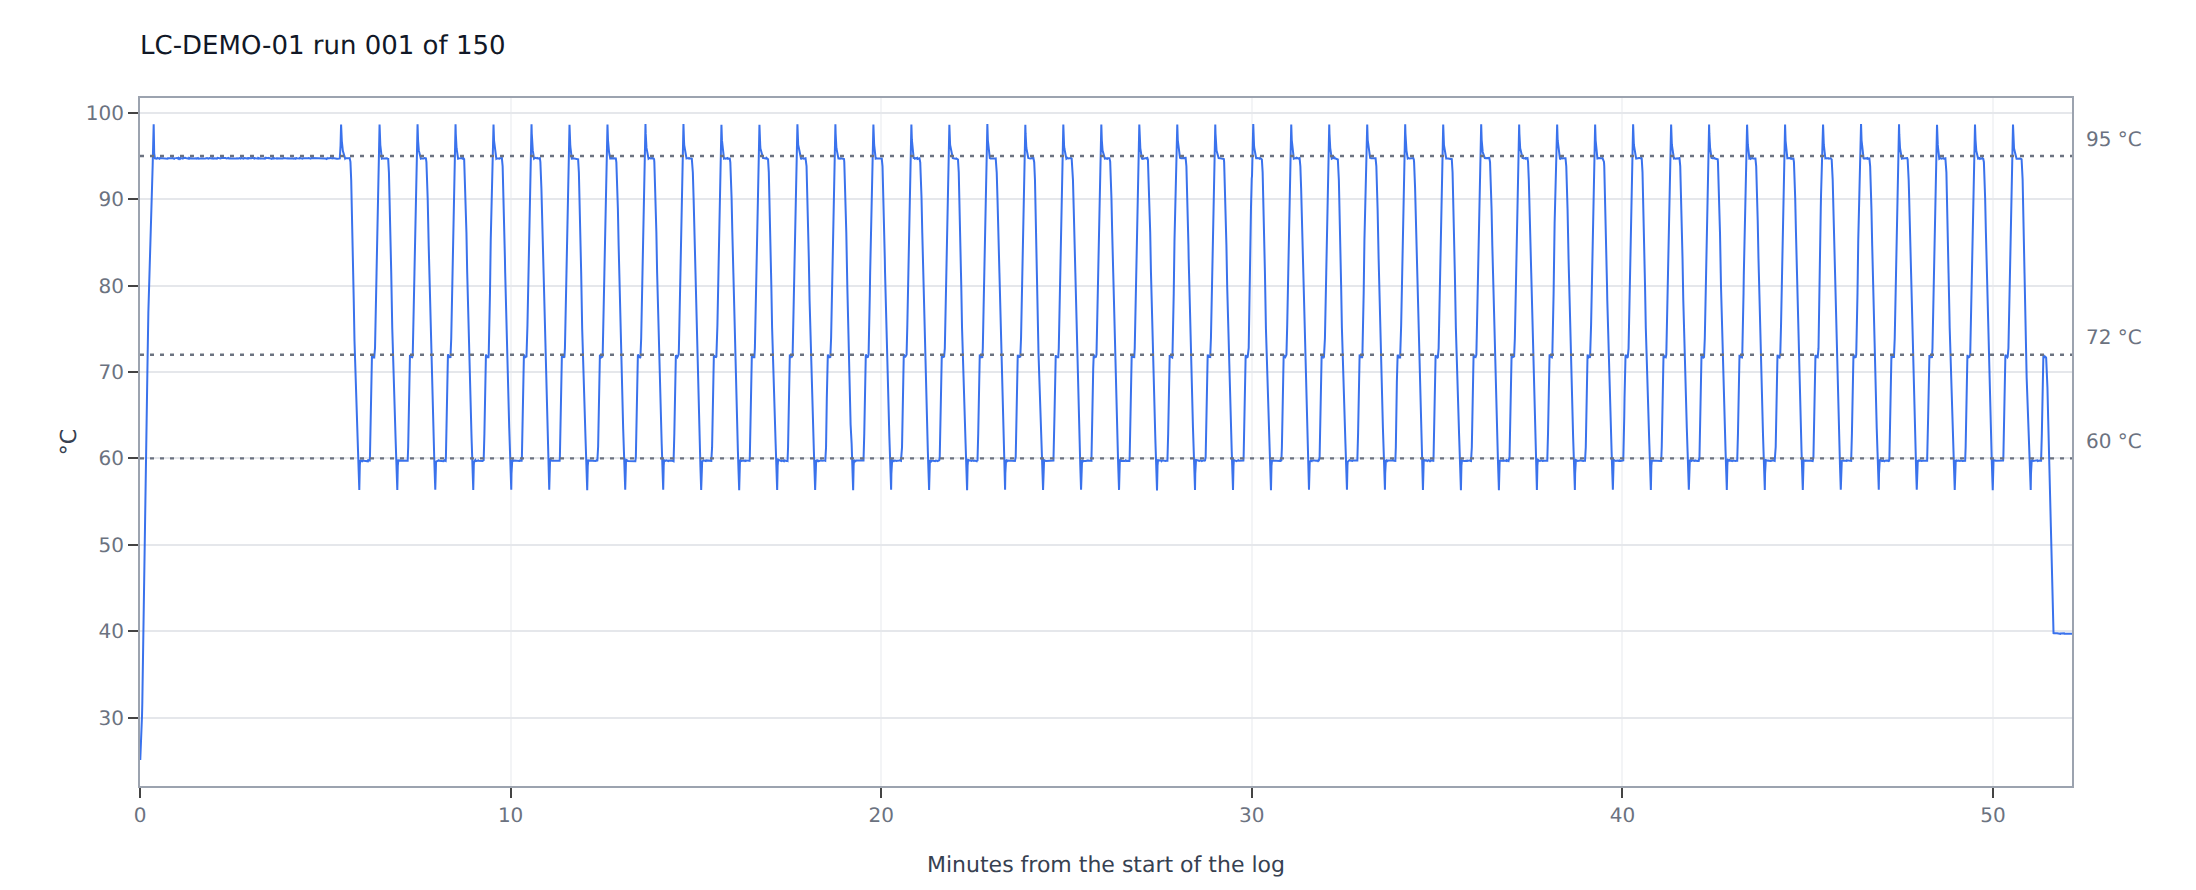
\includegraphics[width=0.92\linewidth,height=0.80\textheight,keepaspectratio]{fig/gallery/graph_lc_thermal.png}
\caption[Block temperature trace (LightCycler temperature log)]{\synthtag Block temperature trace (LightCycler temperature log). {\footnotesize Exercises \texttt{extent}, \texttt{gByDate}, \texttt{gCutLines}, \texttt{gRunTicks}, \texttt{gRunWells}, \texttt{gTargets} and 56 more function(s) reachable from them.}}
\label{fig:gal-graph-lc-thermal}
\end{figure}

\begin{figure}[H]\centering
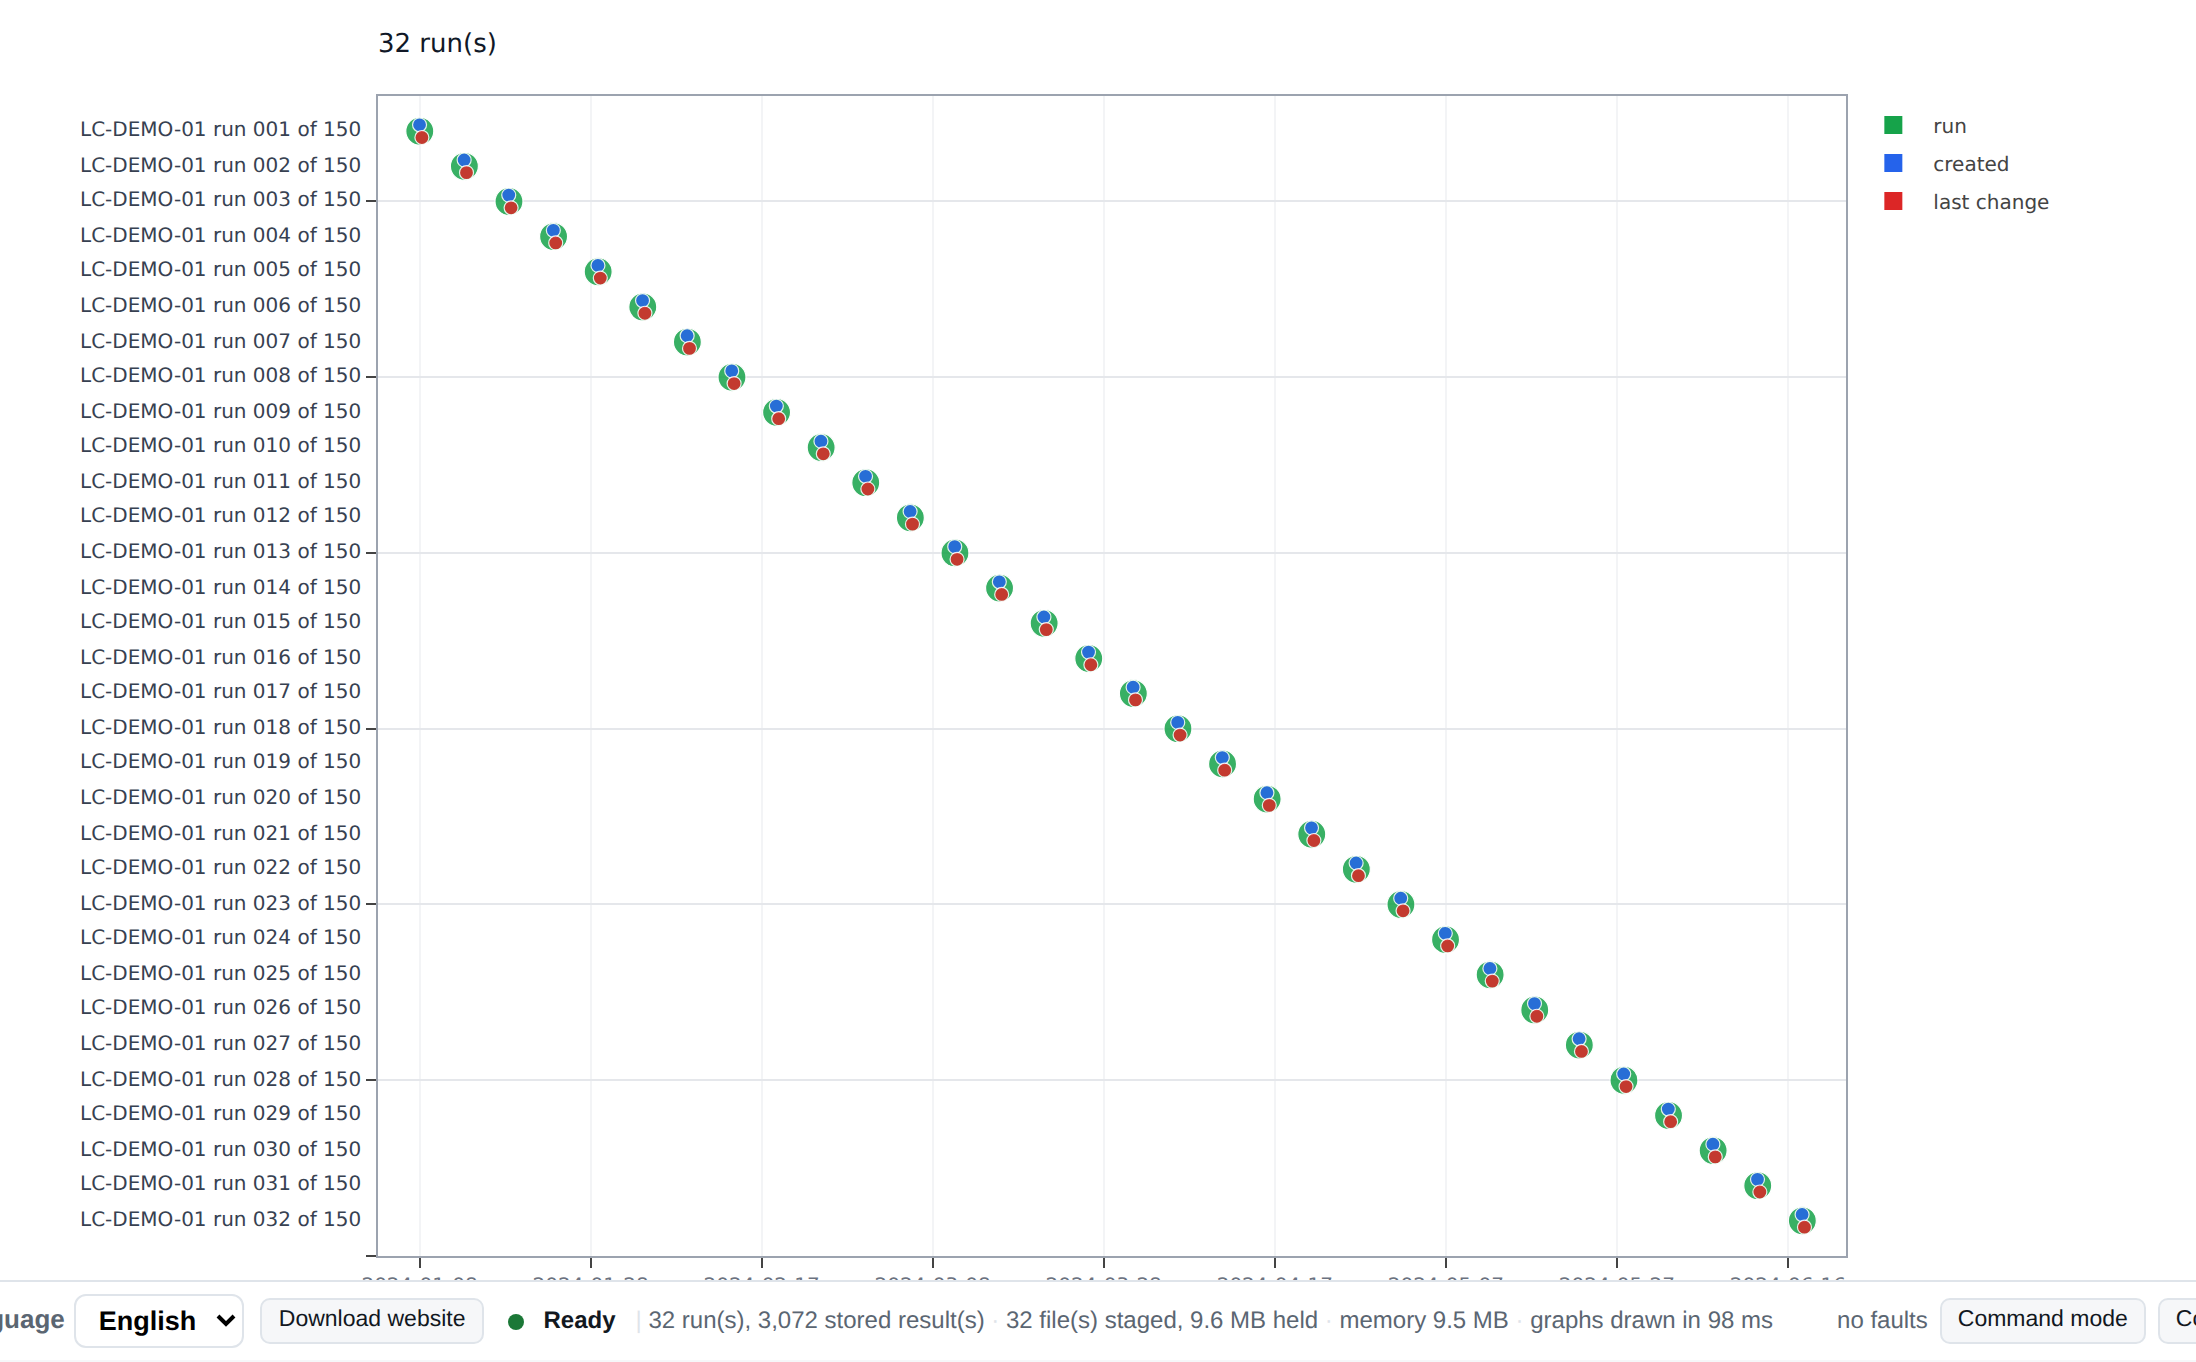
\includegraphics[width=0.92\linewidth,height=0.80\textheight,keepaspectratio]{fig/gallery/graph_x_timeline.png}
\caption[Runs on a calendar — run time and last change]{\synthtag Runs on a calendar — run time and last change. {\footnotesize Exercises \texttt{extent}, \texttt{gByDate}, \texttt{gCutLines}, \texttt{gRunTicks}, \texttt{gRunWells}, \texttt{gTargets} and 56 more function(s) reachable from them.}}
\label{fig:gal-graph-x-timeline}
\end{figure}

\begin{figure}[H]\centering
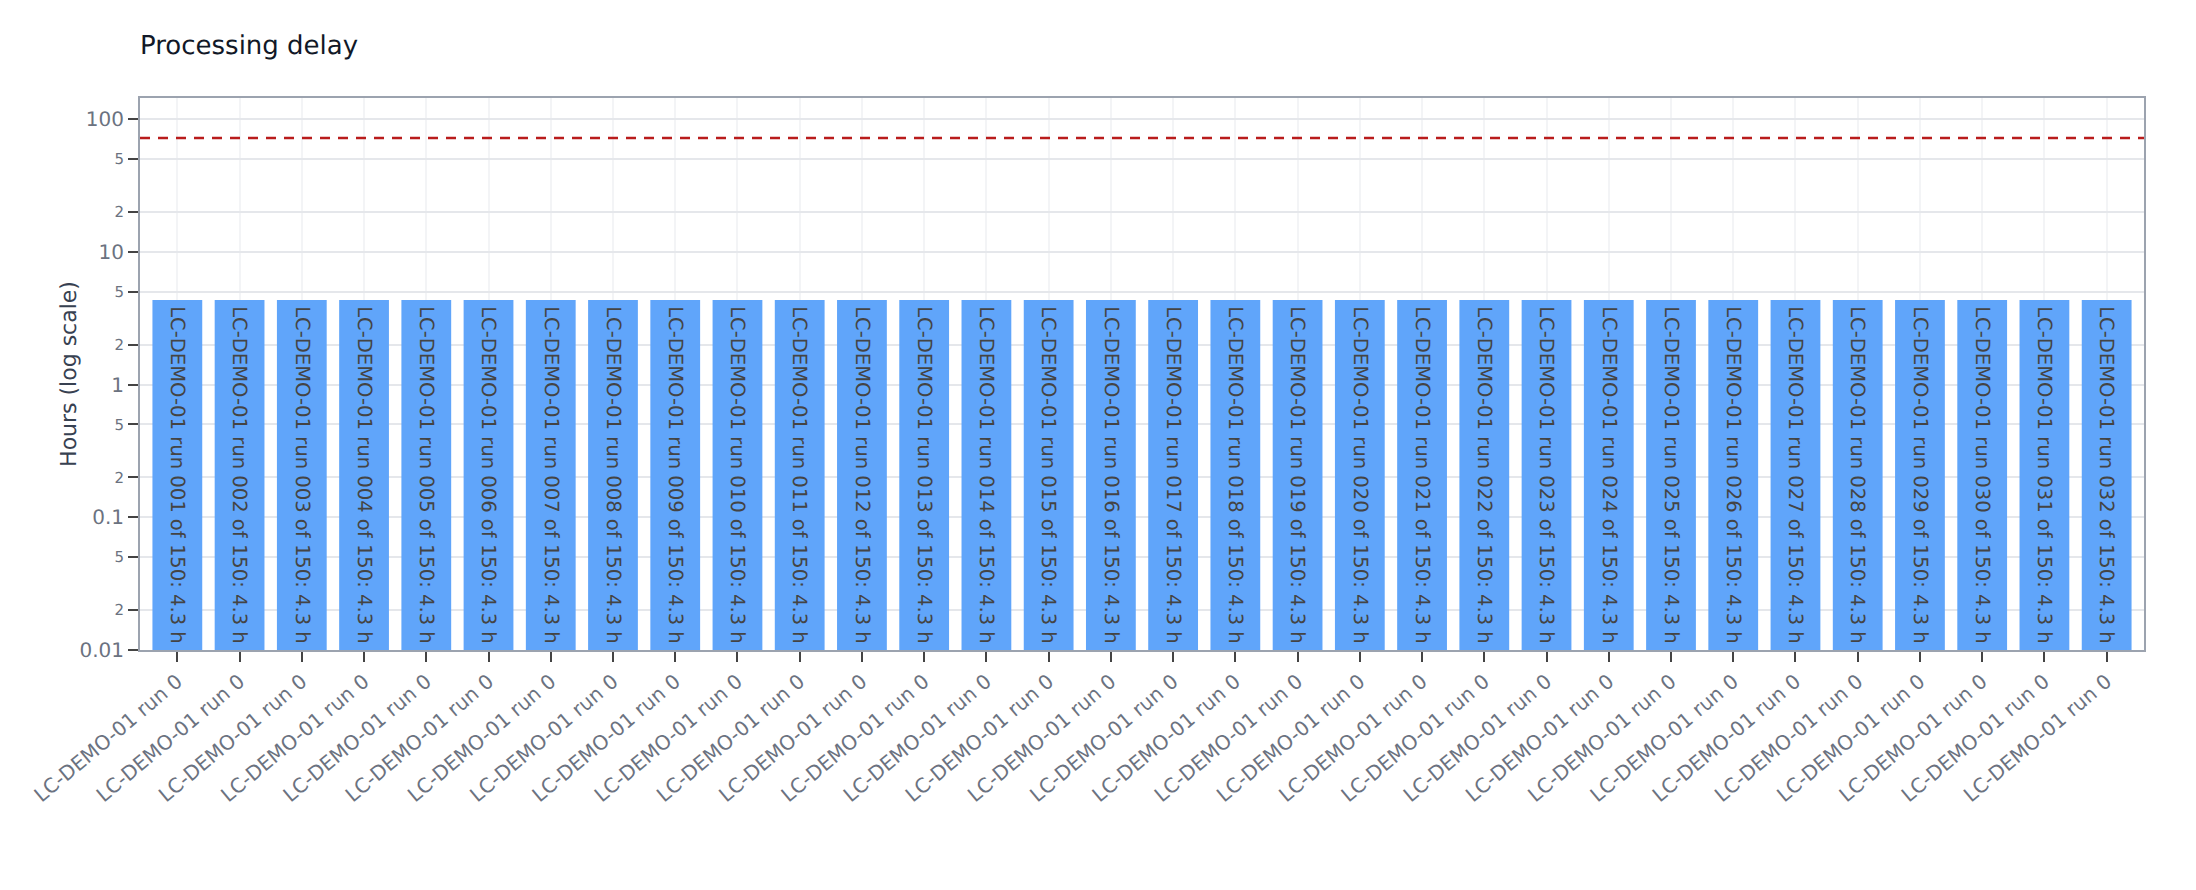
\includegraphics[width=0.92\linewidth,height=0.80\textheight,keepaspectratio]{fig/gallery/graph_x_delay.png}
\caption[Hours from run end to the last recorded change]{\synthtag Hours from run end to the last recorded change. {\footnotesize Exercises \texttt{extent}, \texttt{gByDate}, \texttt{gCutLines}, \texttt{gRunTicks}, \texttt{gRunWells}, \texttt{gTargets} and 56 more function(s) reachable from them.}}
\label{fig:gal-graph-x-delay}
\end{figure}

\begin{figure}[H]\centering
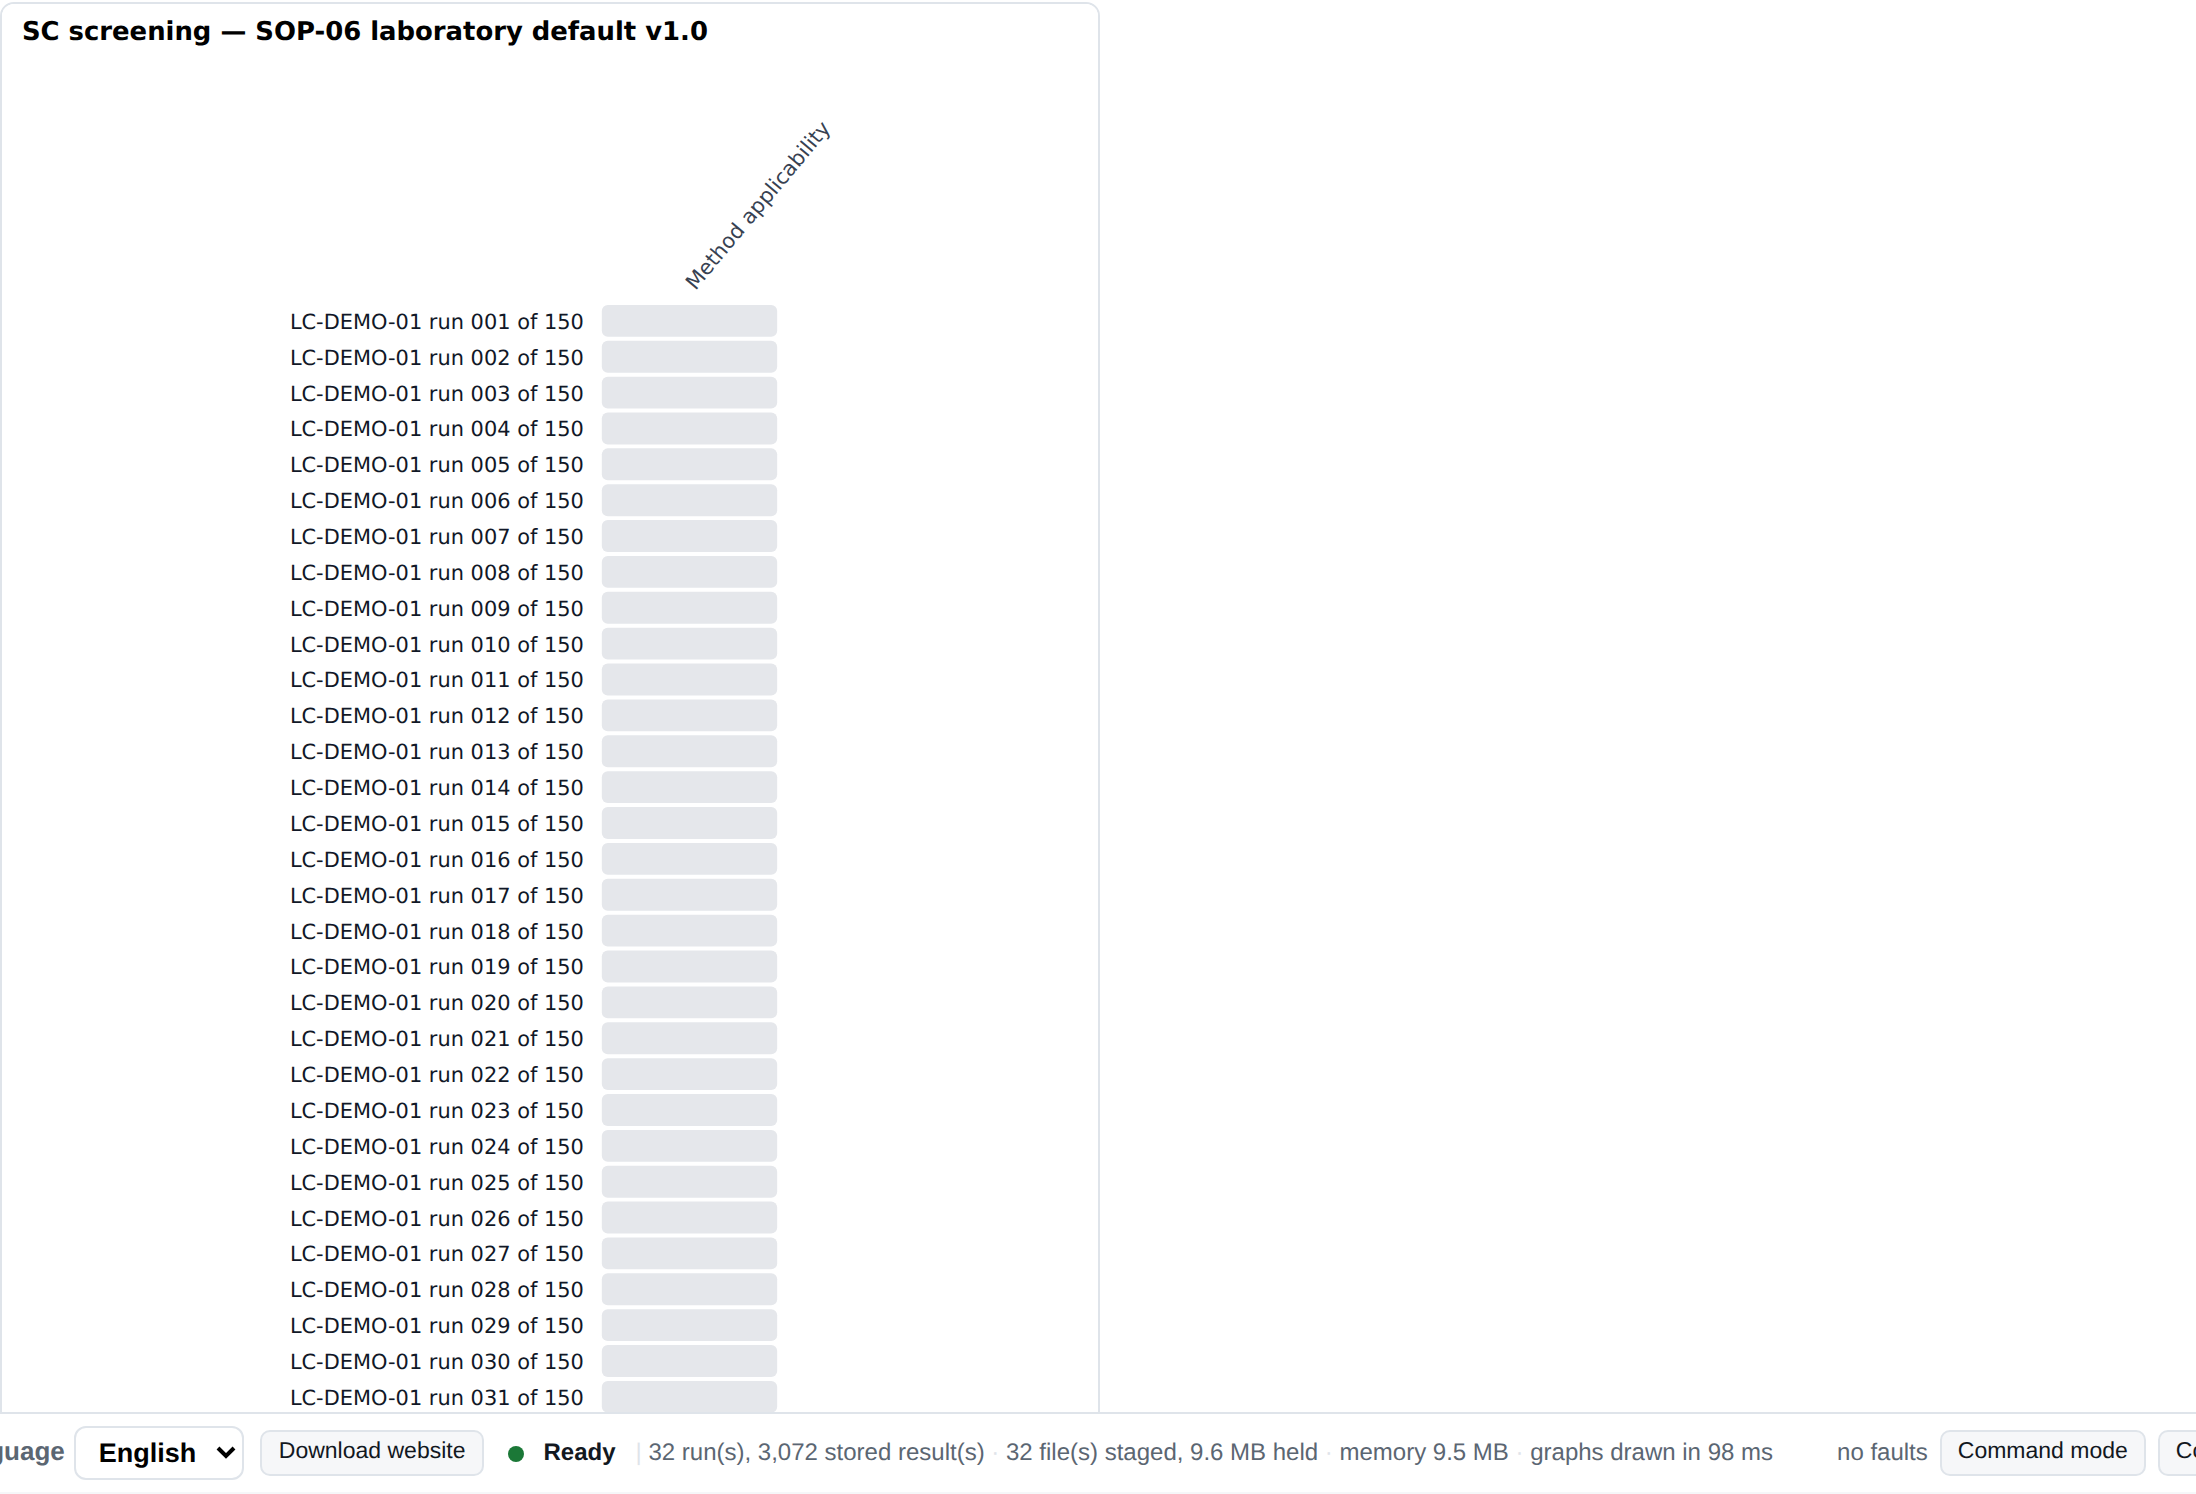
\includegraphics[width=0.92\linewidth,height=0.80\textheight,keepaspectratio]{fig/gallery/graph_x_accept.png}
\caption[Run acceptance grid]{\synthtag Run acceptance grid. {\footnotesize Exercises \texttt{extent}, \texttt{gByDate}, \texttt{gCutLines}, \texttt{gRunTicks}, \texttt{gRunWells}, \texttt{gTargets} and 56 more function(s) reachable from them.}}
\label{fig:gal-graph-x-accept}
\end{figure}

\begin{figure}[H]\centering
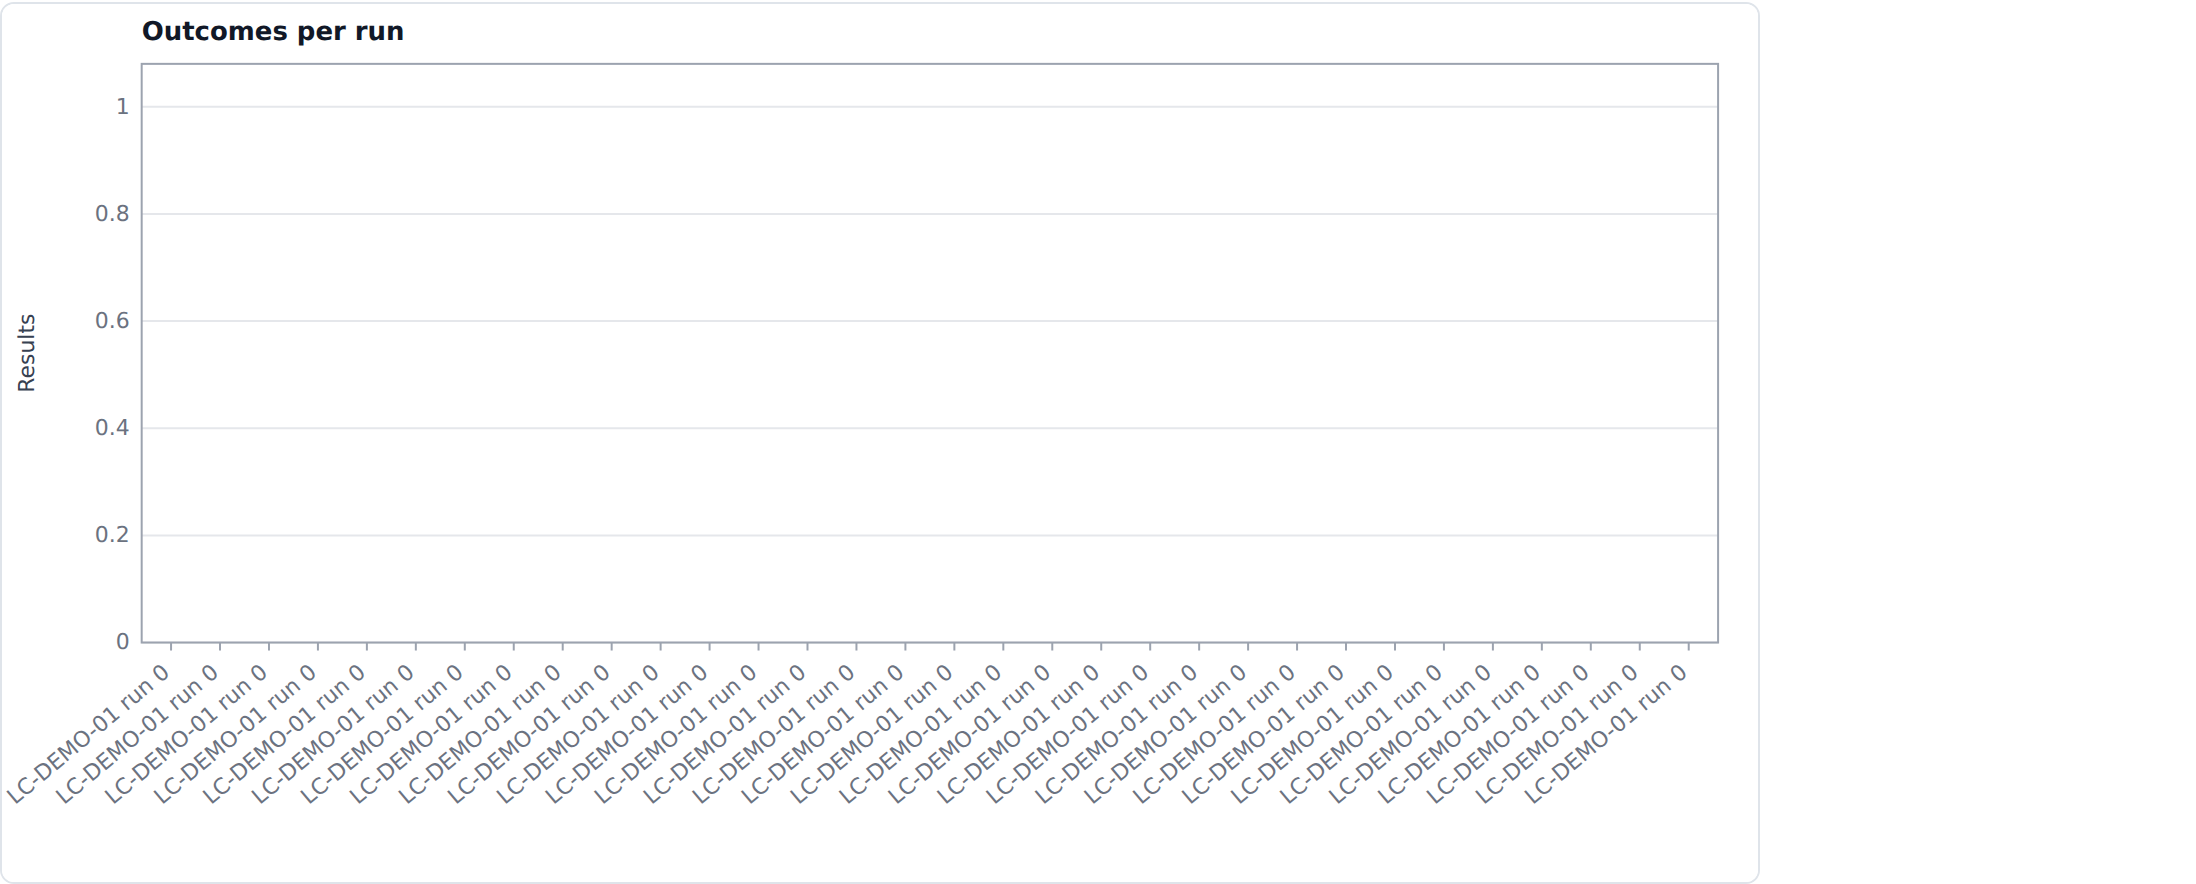
\includegraphics[width=0.92\linewidth,height=0.80\textheight,keepaspectratio]{fig/gallery/graph_x_outcomes.png}
\caption[SOP outcomes per run]{\synthtag SOP outcomes per run. {\footnotesize Exercises \texttt{extent}, \texttt{gByDate}, \texttt{gCutLines}, \texttt{gRunTicks}, \texttt{gRunWells}, \texttt{gTargets} and 56 more function(s) reachable from them.}}
\label{fig:gal-graph-x-outcomes}
\end{figure}

\begin{figure}[H]\centering

\includegraphics[width=0.92\linewidth,height=0.80\textheight,keepaspectratio]{fig/gallery/graph_x_control.png}
\caption[Control Cq across runs with SOP range --- no data for this view in the demonstration set]{\synthtag Control Cq across runs with SOP range --- no data for this view in the demonstration set. {\footnotesize Exercises \texttt{extent}, \texttt{gByDate}, \texttt{gCutLines}, \texttt{gRunTicks}, \texttt{gRunWells}, \texttt{gTargets} and 56 more function(s) reachable from them.}}
\label{fig:gal-graph-x-control}
\end{figure}

\begin{figure}[H]\centering
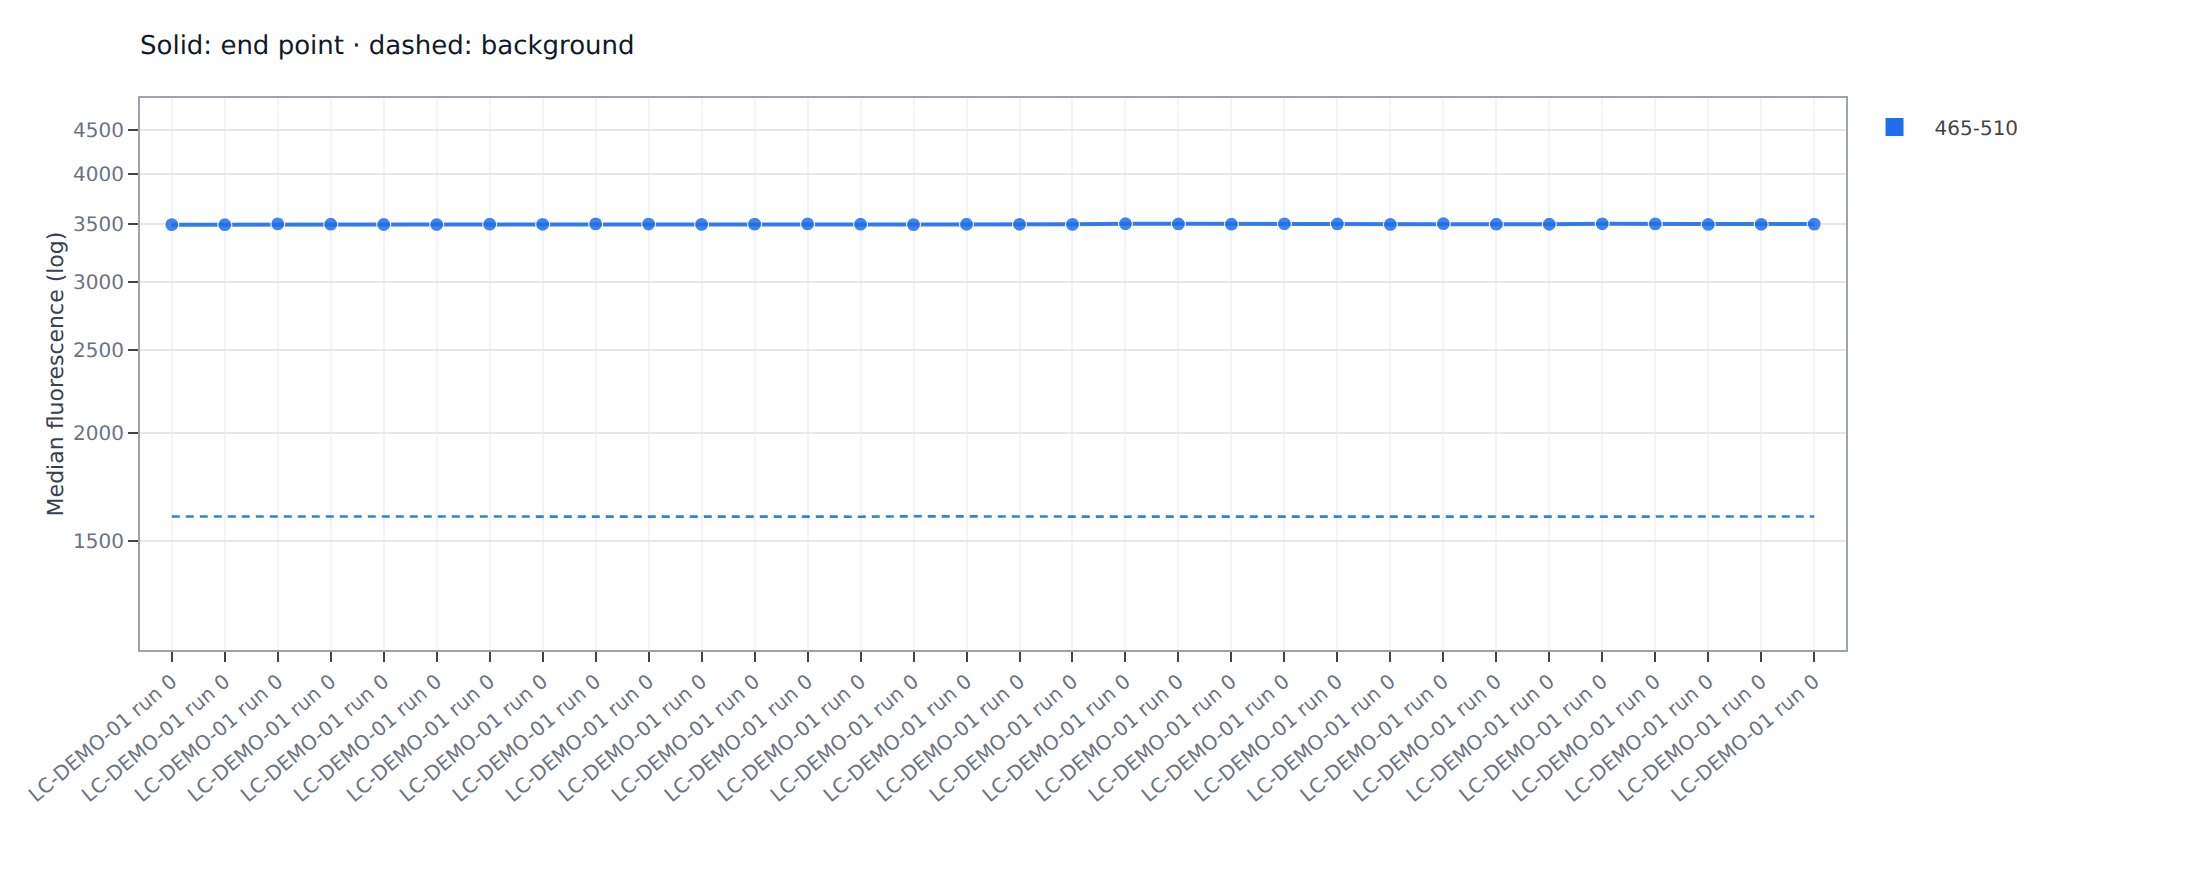
\includegraphics[width=0.92\linewidth,height=0.80\textheight,keepaspectratio]{fig/gallery/graph_x_signal.png}
\caption[Background and plateau fluorescence across runs]{\synthtag Background and plateau fluorescence across runs. {\footnotesize Exercises \texttt{extent}, \texttt{gByDate}, \texttt{gCutLines}, \texttt{gRunTicks}, \texttt{gRunWells}, \texttt{gTargets} and 56 more function(s) reachable from them.}}
\label{fig:gal-graph-x-signal}
\end{figure}

\begin{figure}[H]\centering
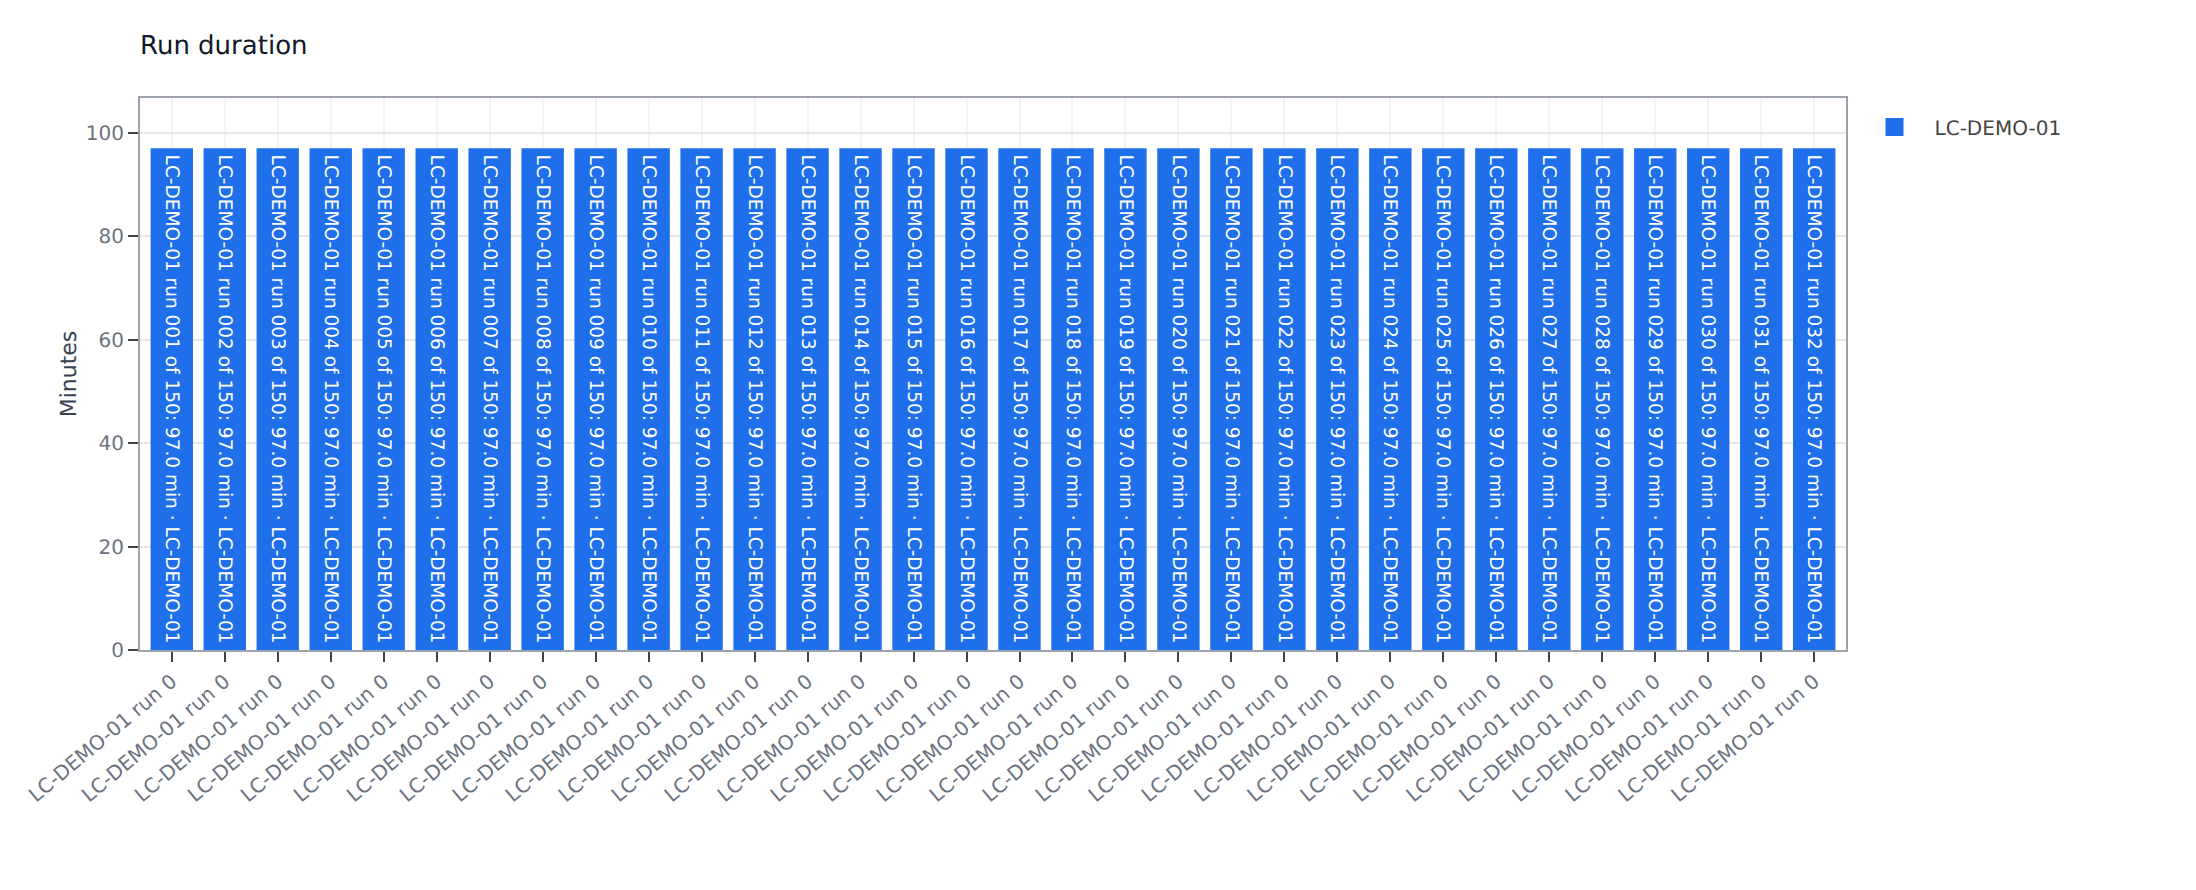
\includegraphics[width=0.92\linewidth,height=0.80\textheight,keepaspectratio]{fig/gallery/graph_x_duration.png}
\caption[Run duration and instrument use]{\synthtag Run duration and instrument use. {\footnotesize Exercises \texttt{extent}, \texttt{gByDate}, \texttt{gCutLines}, \texttt{gRunTicks}, \texttt{gRunWells}, \texttt{gTargets} and 56 more function(s) reachable from them.}}
\label{fig:gal-graph-x-duration}
\end{figure}

\begin{figure}[H]\centering
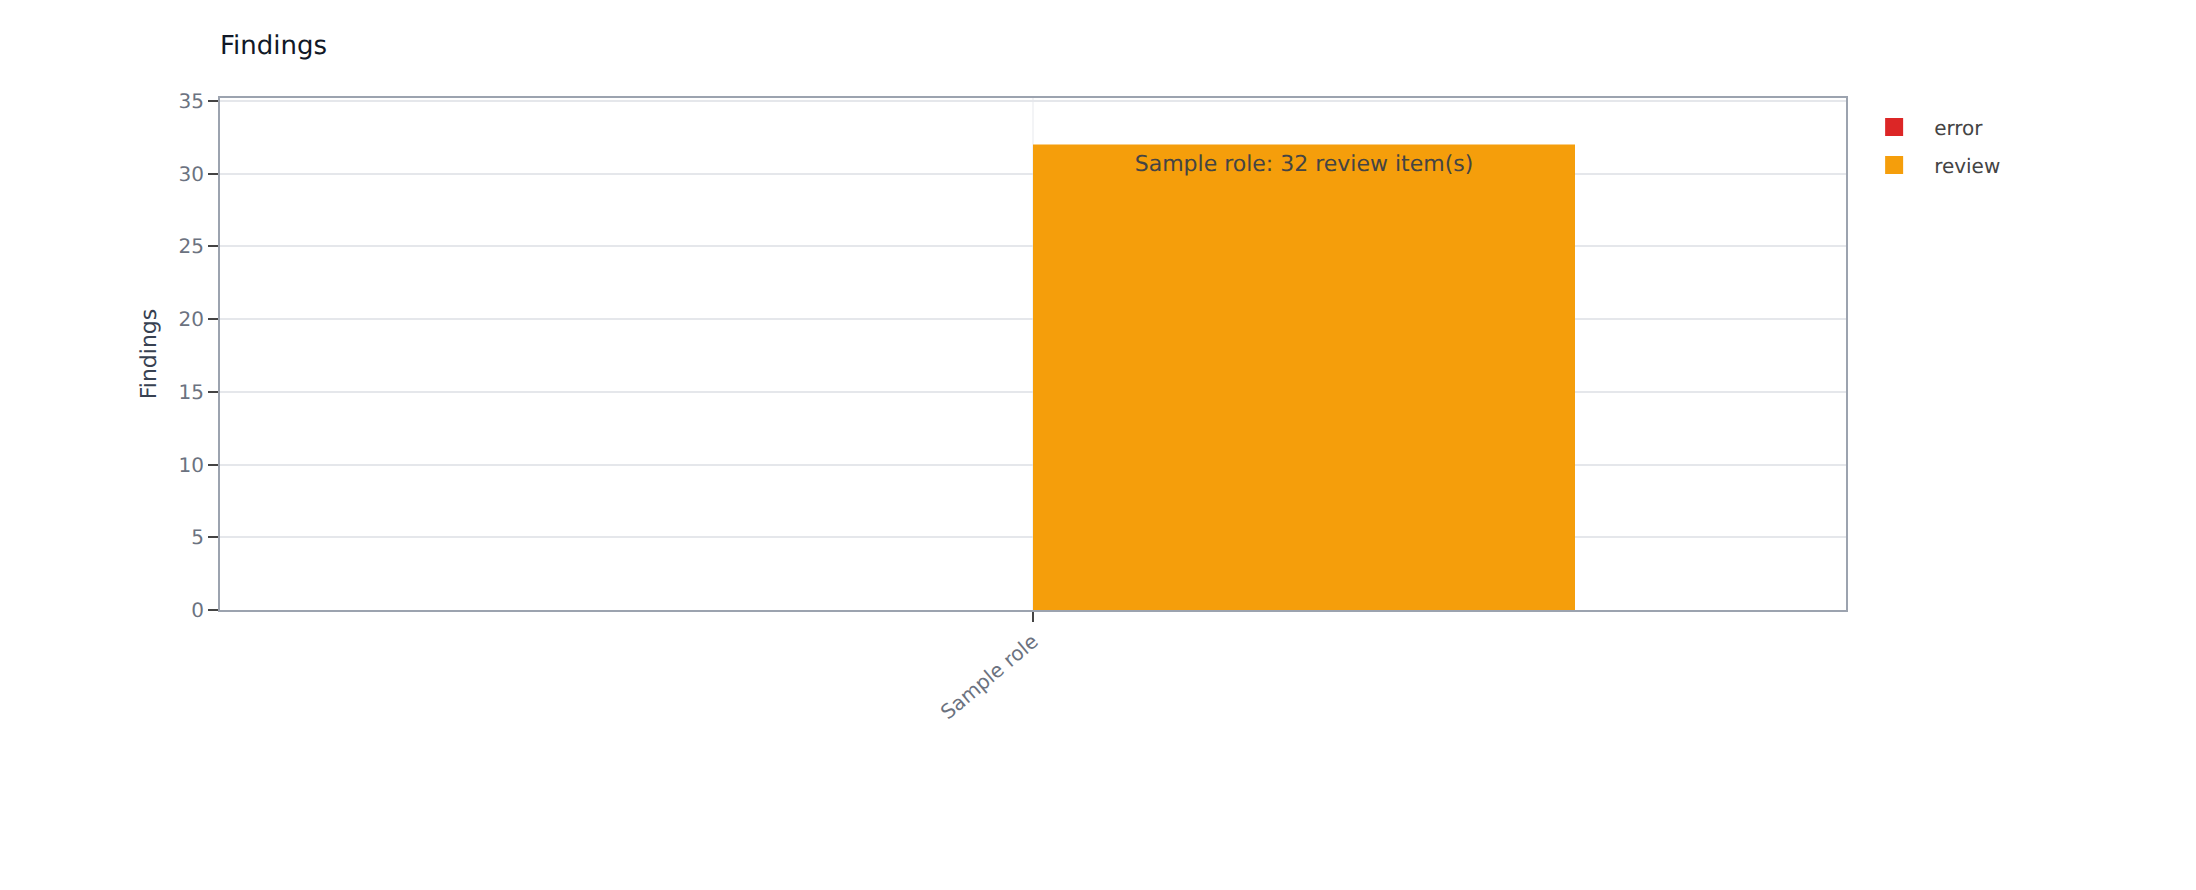
\includegraphics[width=0.92\linewidth,height=0.80\textheight,keepaspectratio]{fig/gallery/graph_x_findings.png}
\caption[Forensic findings by area (Pareto)]{\synthtag Forensic findings by area (Pareto). {\footnotesize Exercises \texttt{extent}, \texttt{gByDate}, \texttt{gCutLines}, \texttt{gRunTicks}, \texttt{gRunWells}, \texttt{gTargets} and 56 more function(s) reachable from them.}}
\label{fig:gal-graph-x-findings}
\end{figure}

\begin{figure}[H]\centering

\includegraphics[width=0.92\linewidth,height=0.80\textheight,keepaspectratio]{fig/gallery/graph_x_control_batches.png}
\caption[Control extraction batches --- no data for this view in the demonstration set]{\synthtag Control extraction batches --- no data for this view in the demonstration set. {\footnotesize Exercises \texttt{controlBatchGraph}, \texttt{controlBatchRecords}, \texttt{extent}, \texttt{gByDate}, \texttt{gCutLines}, \texttt{gRunTicks} and 69 more function(s) reachable from them.}}
\label{fig:gal-graph-x-control-batches}
\end{figure}

\begin{figure}[H]\centering

\includegraphics[width=0.92\linewidth,height=0.80\textheight,keepaspectratio]{fig/gallery/graph_x_control_age.png}
\caption[Control extract age versus Cq --- no data for this view in the demonstration set]{\synthtag Control extract age versus Cq --- no data for this view in the demonstration set. {\footnotesize Exercises \texttt{controlBatchGraph}, \texttt{controlBatchRecords}, \texttt{extent}, \texttt{gByDate}, \texttt{gCutLines}, \texttt{gRunTicks} and 69 more function(s) reachable from them.}}
\label{fig:gal-graph-x-control-age}
\end{figure}

\begin{figure}[H]\centering

\includegraphics[width=0.92\linewidth,height=0.80\textheight,keepaspectratio]{fig/gallery/graph_x_control_thermal.png}
\caption[Control Cq versus cooling rate --- no data for this view in the demonstration set]{\synthtag Control Cq versus cooling rate --- no data for this view in the demonstration set. {\footnotesize Exercises \texttt{controlBatchGraph}, \texttt{controlBatchRecords}, \texttt{extent}, \texttt{gByDate}, \texttt{gCutLines}, \texttt{gRunTicks} and 69 more function(s) reachable from them.}}
\label{fig:gal-graph-x-control-thermal}
\end{figure}

\section{The control panel in control}
LC-DEMO-01 over thirty-two runs. Nineteen charts have data and are in control; one asks for a second look at a pattern inside the limits.

\begin{figure}[H]\centering
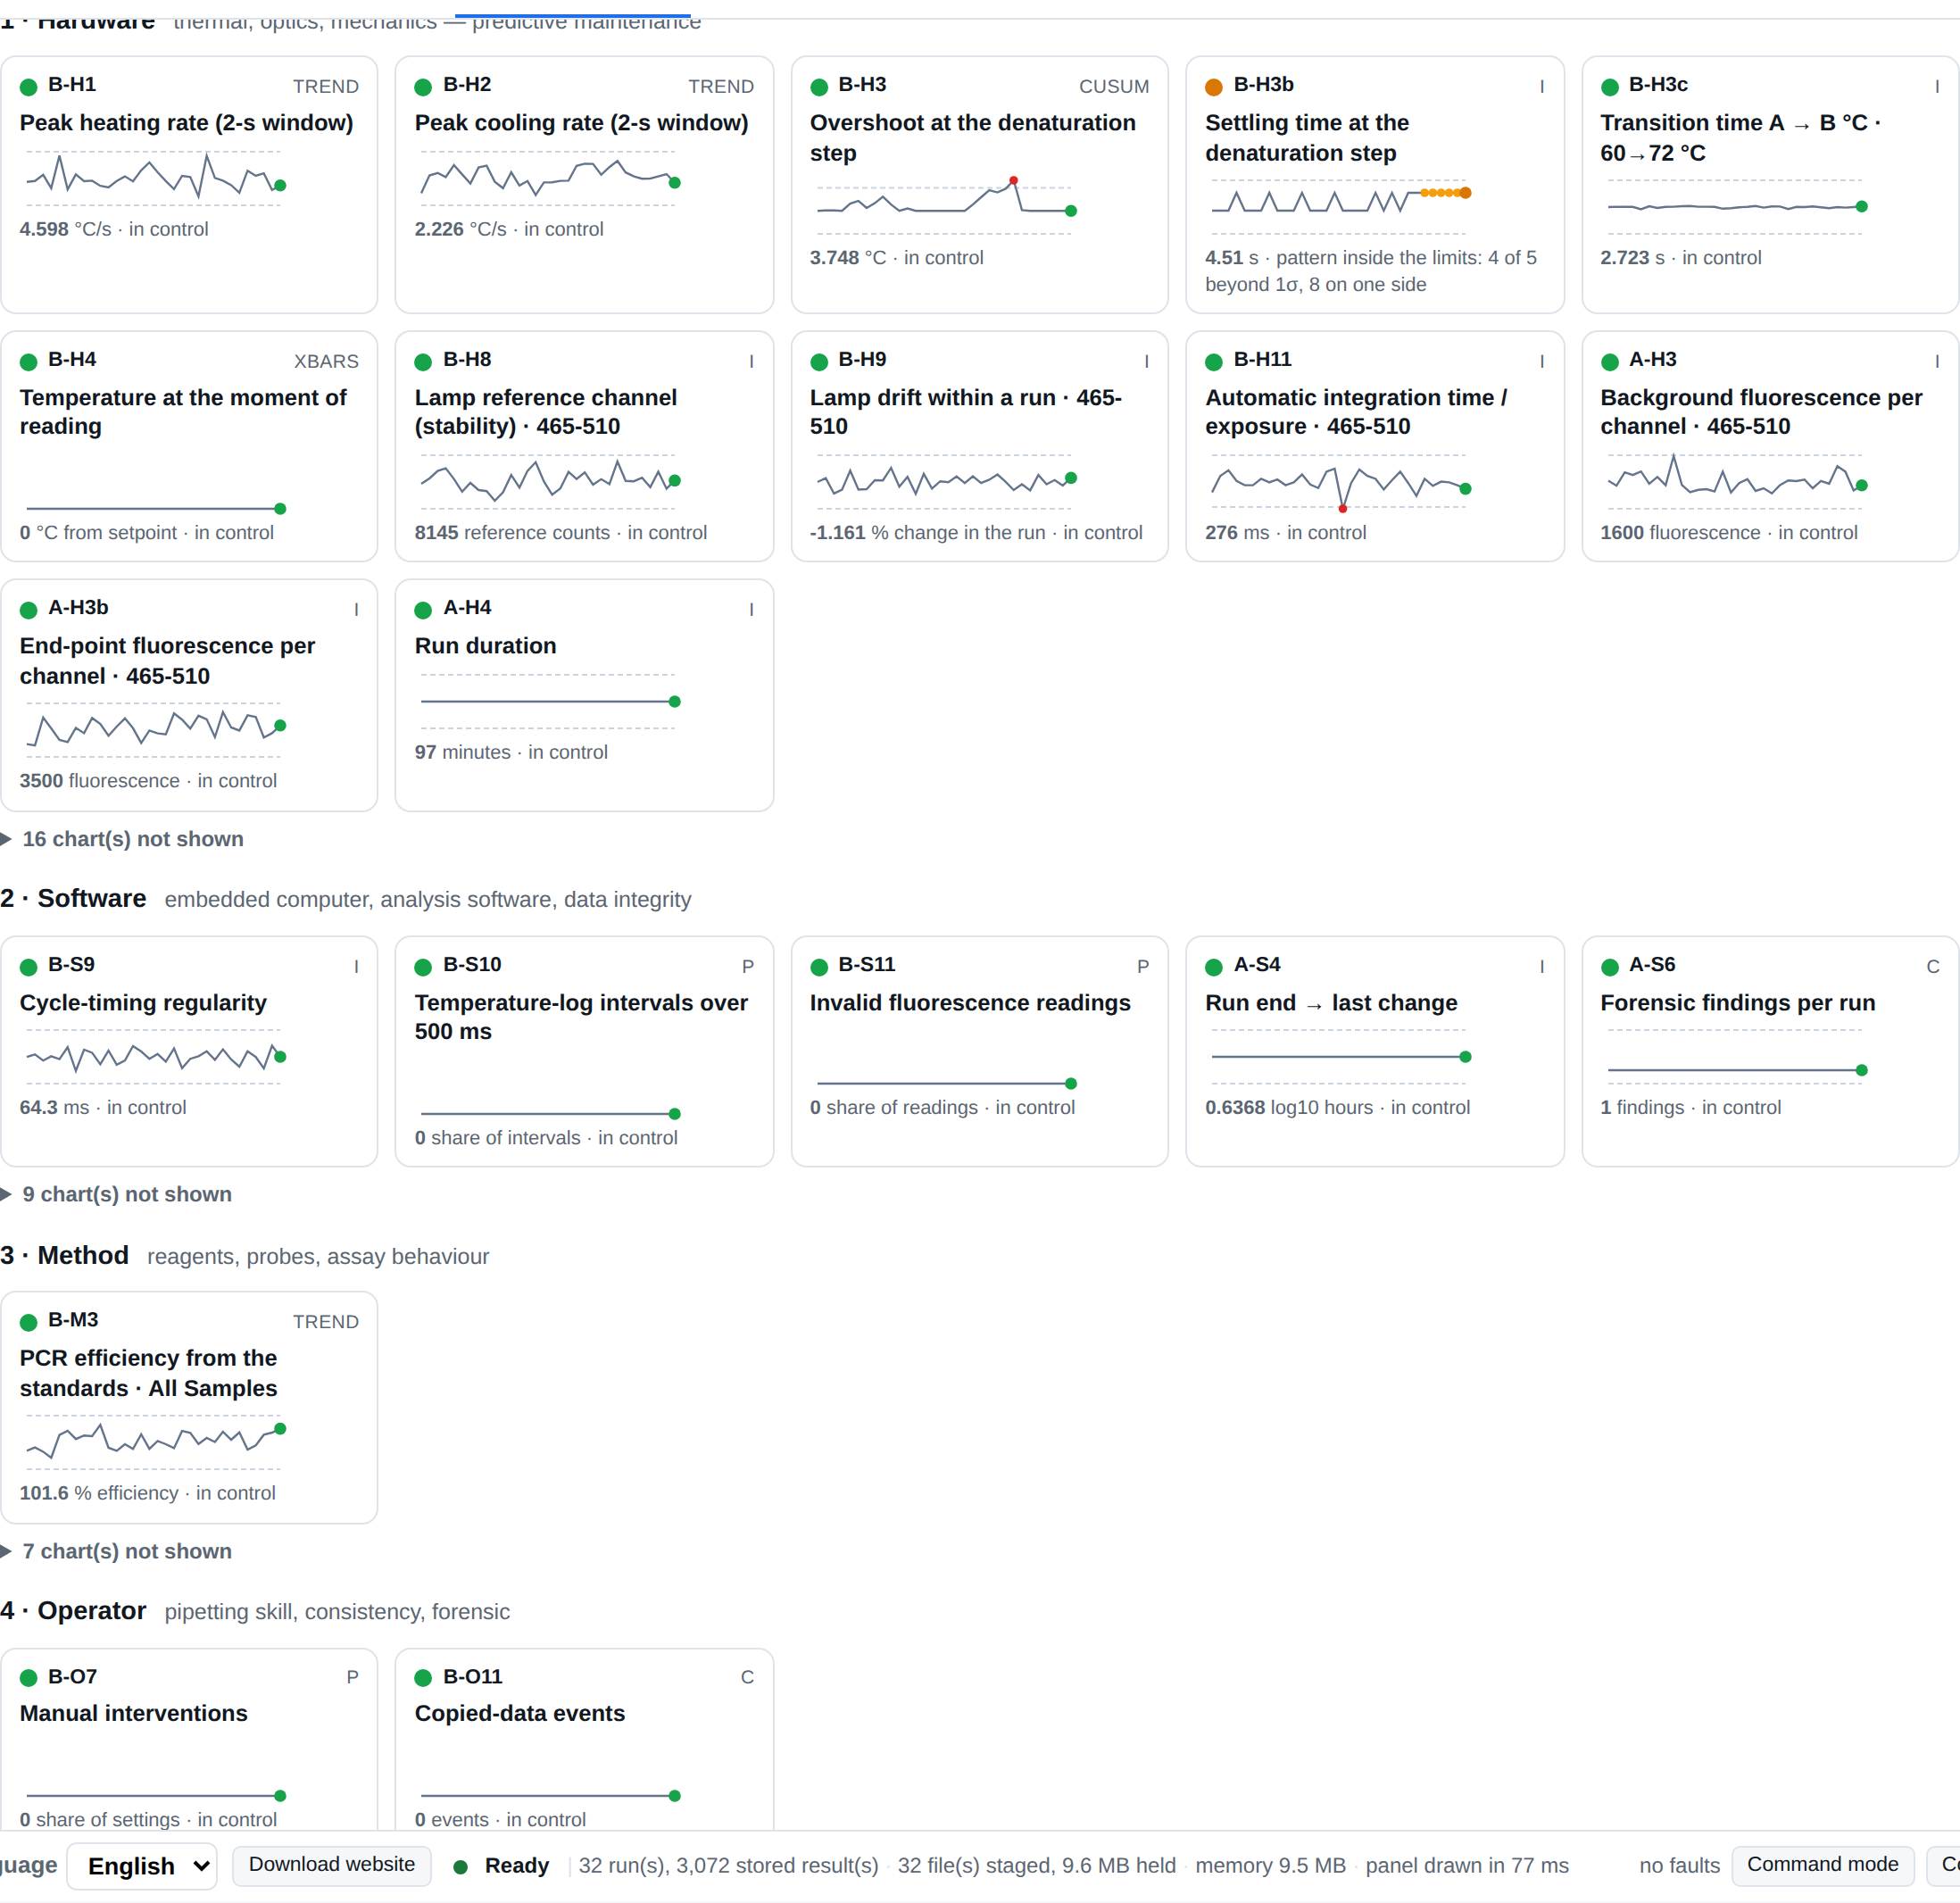
\includegraphics[width=0.98\linewidth,height=0.80\textheight,keepaspectratio]{fig/gallery/cc_overview.png}
\caption[Control panel overview: one card per chart, with its status]{\synthtag Control panel overview: one card per chart, with its status. {\footnotesize Exercises \texttt{ccCompute}, \texttt{ccRowsFor}, \texttt{ccStatus}, \texttt{ccVariants}, \texttt{renderPanel} and 128 more function(s) reachable from them.}}
\label{fig:gal-cc-overview}
\end{figure}

\begin{figure}[H]\centering
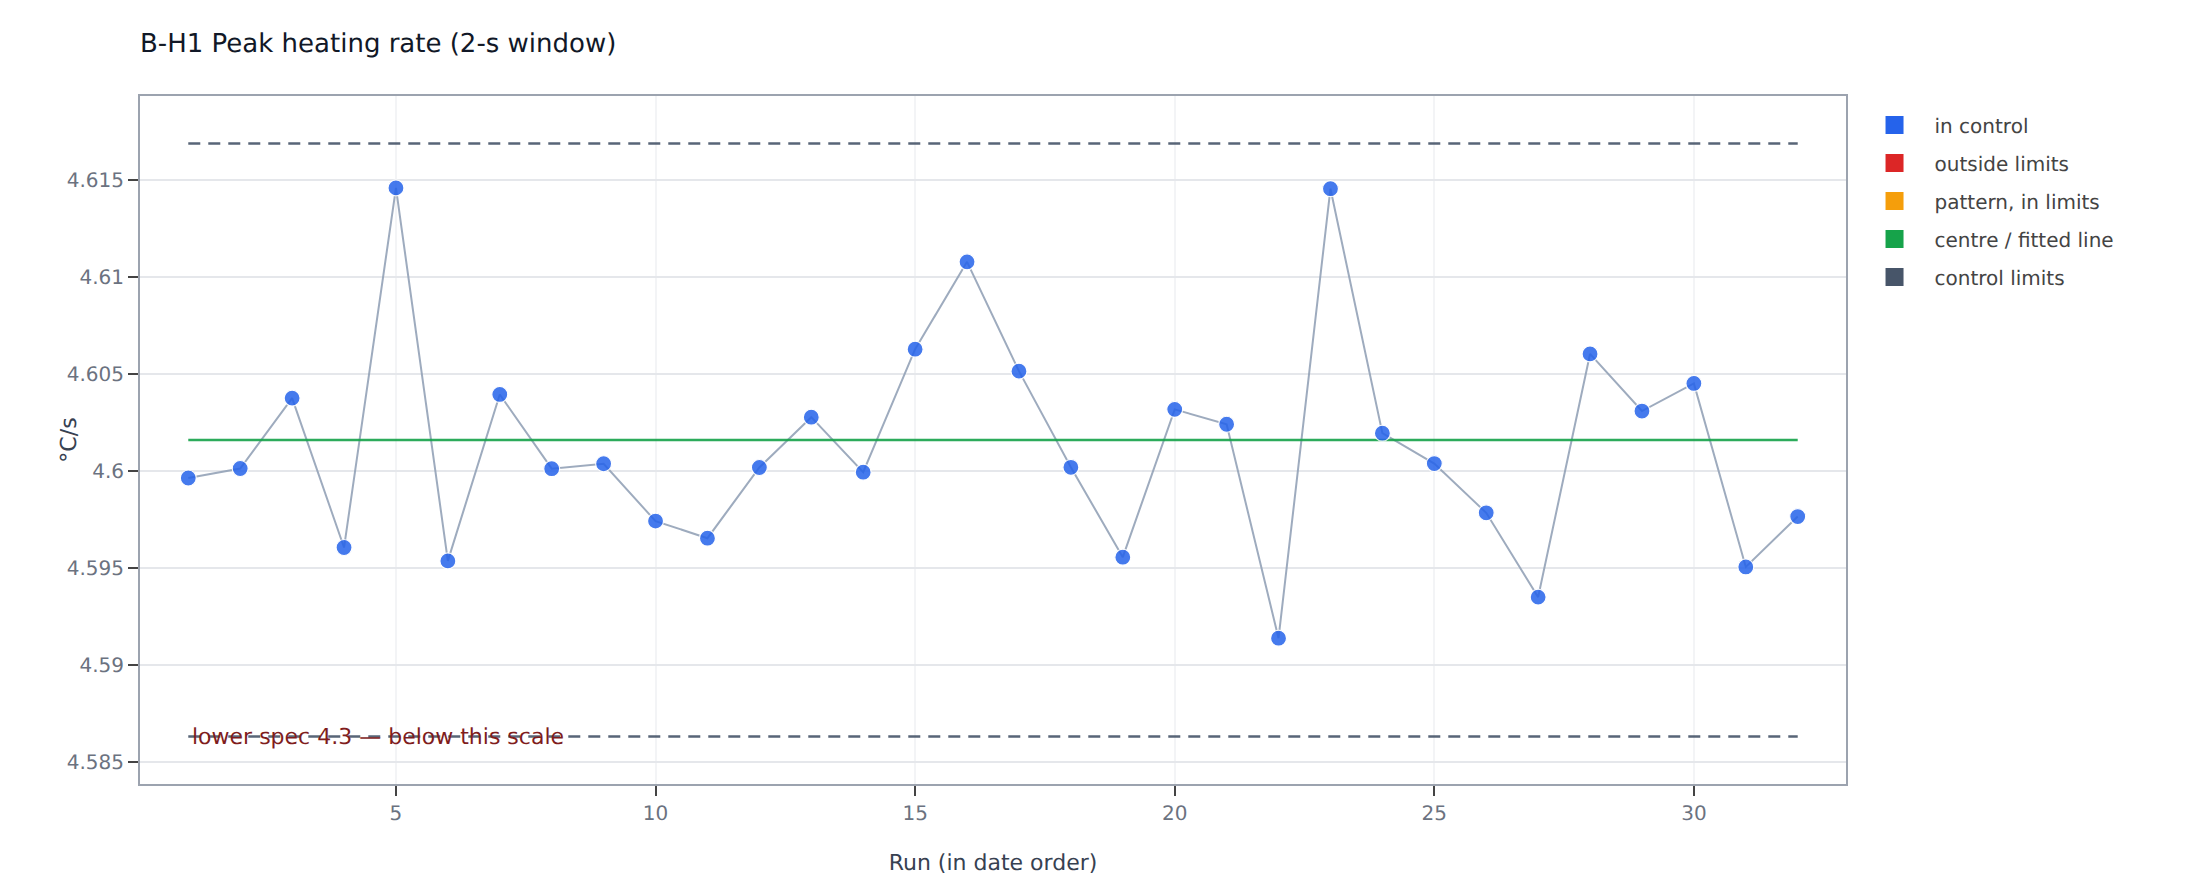
\includegraphics[width=0.92\linewidth,height=0.80\textheight,keepaspectratio]{fig/gallery/cc_type_trend.png}
\caption[B-H1 Peak heating rate (2-s window) — trend chart --- in control]{\synthtag B-H1 Peak heating rate (2-s window) — trend chart --- in control. {\footnotesize Exercises \texttt{ccChartSvg}, \texttt{ccCompute}, \texttt{ixMount}, \texttt{renderCcDetail}, \texttt{svgPlot} and 128 more function(s) reachable from them.}}
\label{fig:gal-cc-type-trend}
\end{figure}

\begin{figure}[H]\centering
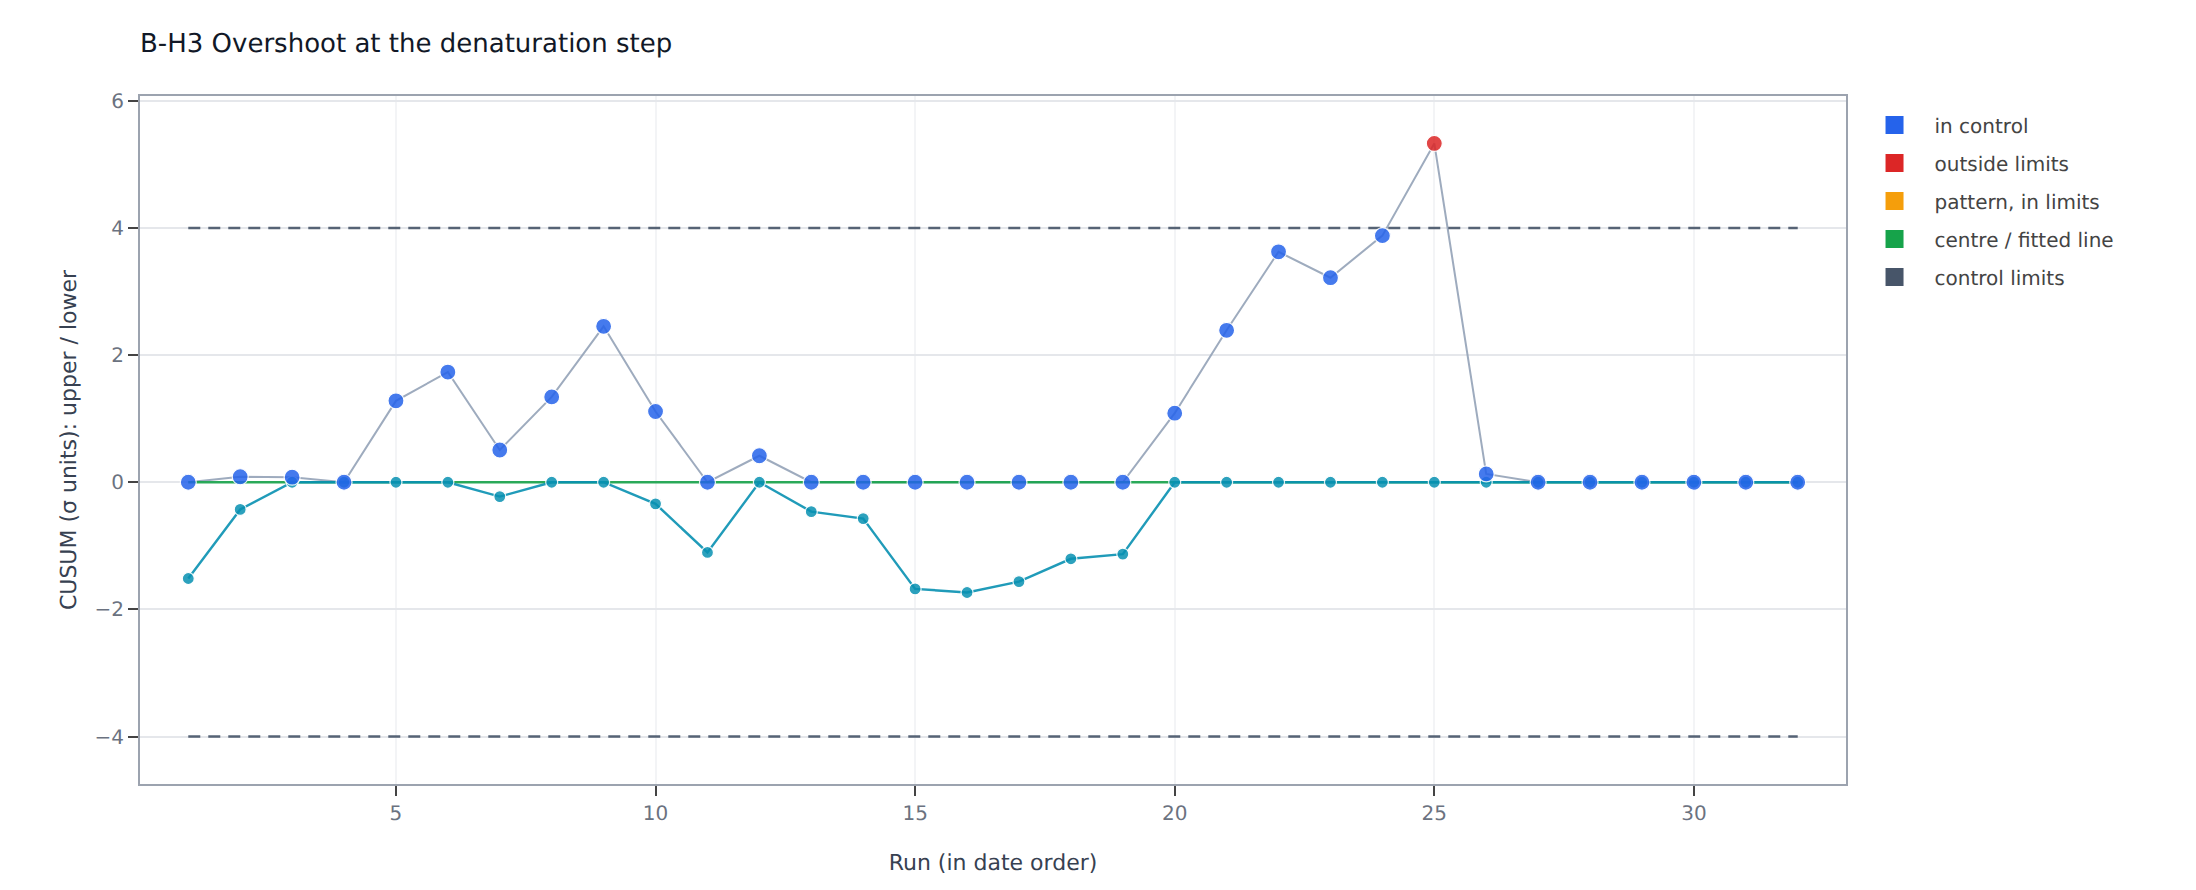
\includegraphics[width=0.92\linewidth,height=0.80\textheight,keepaspectratio]{fig/gallery/cc_type_cusum.png}
\caption[B-H3 Overshoot at the denaturation step — cusum chart --- in control]{\synthtag B-H3 Overshoot at the denaturation step — cusum chart --- in control. {\footnotesize Exercises \texttt{ccChartSvg}, \texttt{ccCompute}, \texttt{ixMount}, \texttt{renderCcDetail}, \texttt{svgPlot} and 128 more function(s) reachable from them.}}
\label{fig:gal-cc-type-cusum}
\end{figure}

\begin{figure}[H]\centering
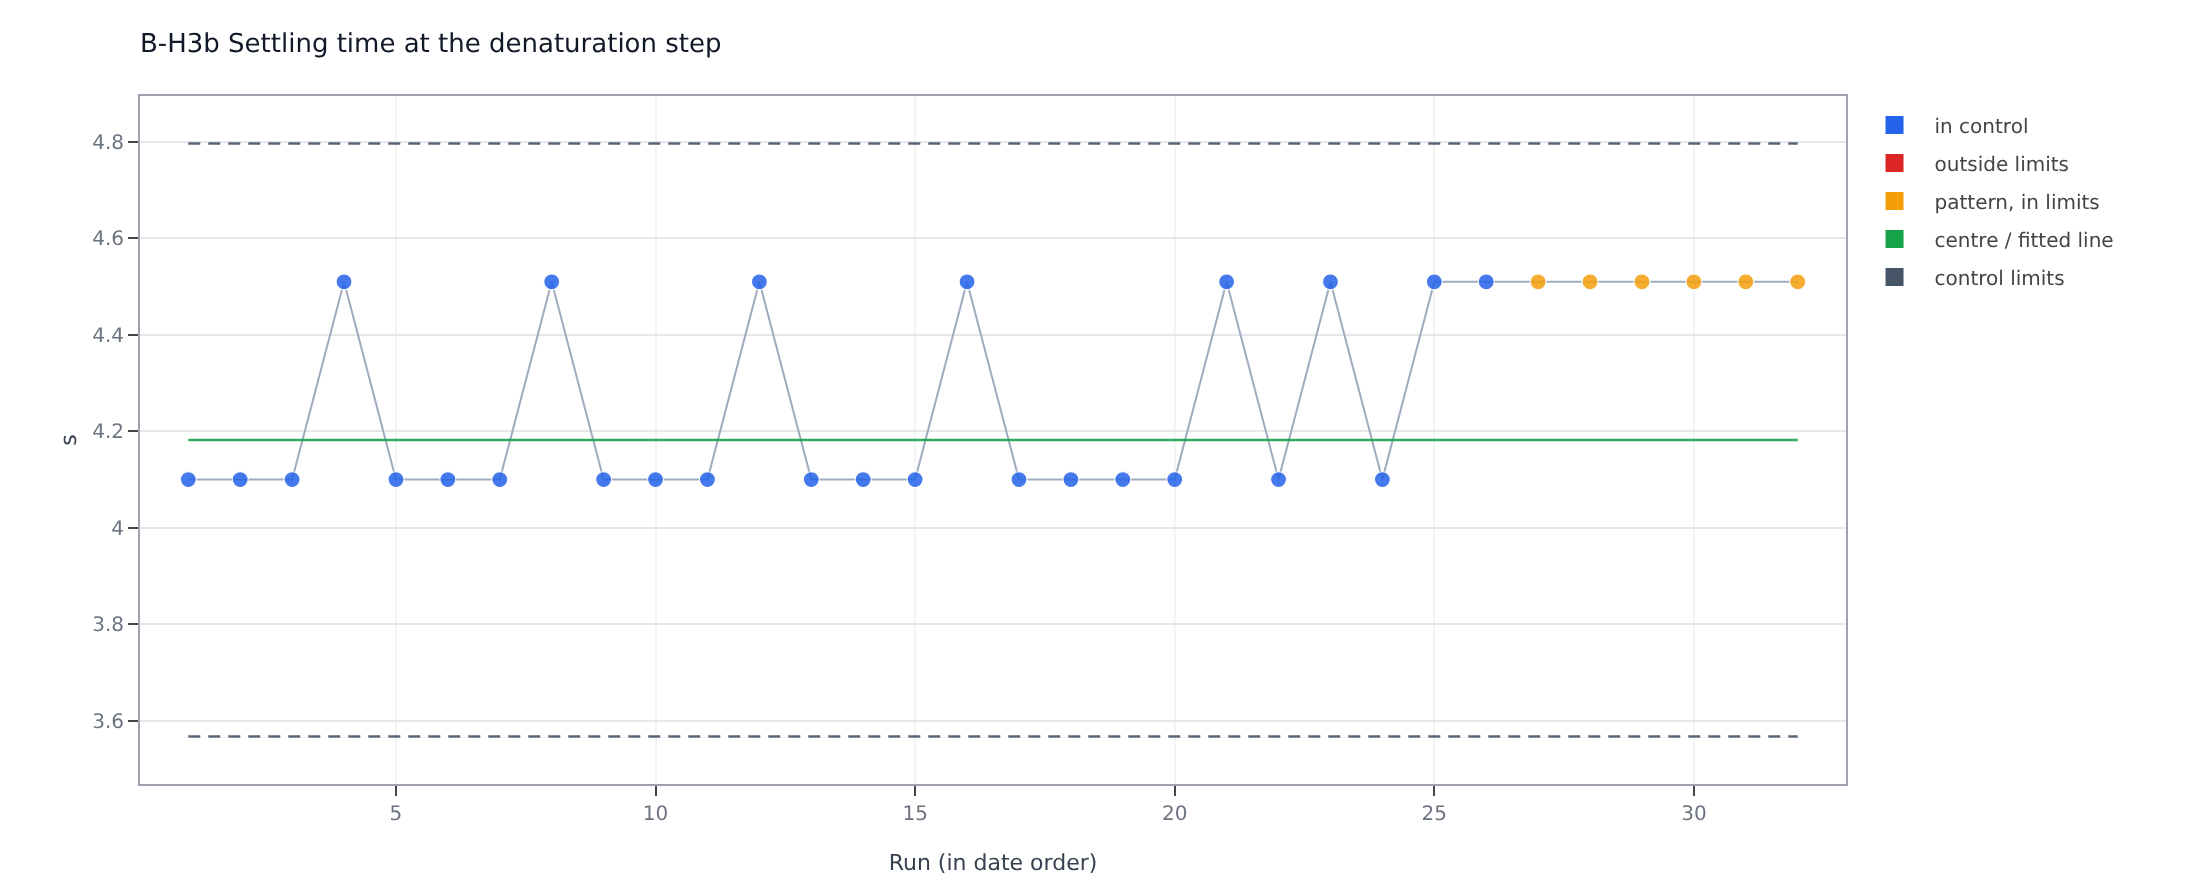
\includegraphics[width=0.92\linewidth,height=0.80\textheight,keepaspectratio]{fig/gallery/cc_type_i.png}
\caption[B-H3b Settling time at the denaturation step — i chart --- pattern inside the limits: 4 of 5 beyond 1σ, 8 on one side]{\synthtag B-H3b Settling time at the denaturation step — i chart --- pattern inside the limits: 4 of 5 beyond 1σ, 8 on one side. {\footnotesize Exercises \texttt{ccChartSvg}, \texttt{ccCompute}, \texttt{ixMount}, \texttt{renderCcDetail}, \texttt{svgPlot} and 128 more function(s) reachable from them.}}
\label{fig:gal-cc-type-i}
\end{figure}

\begin{figure}[H]\centering
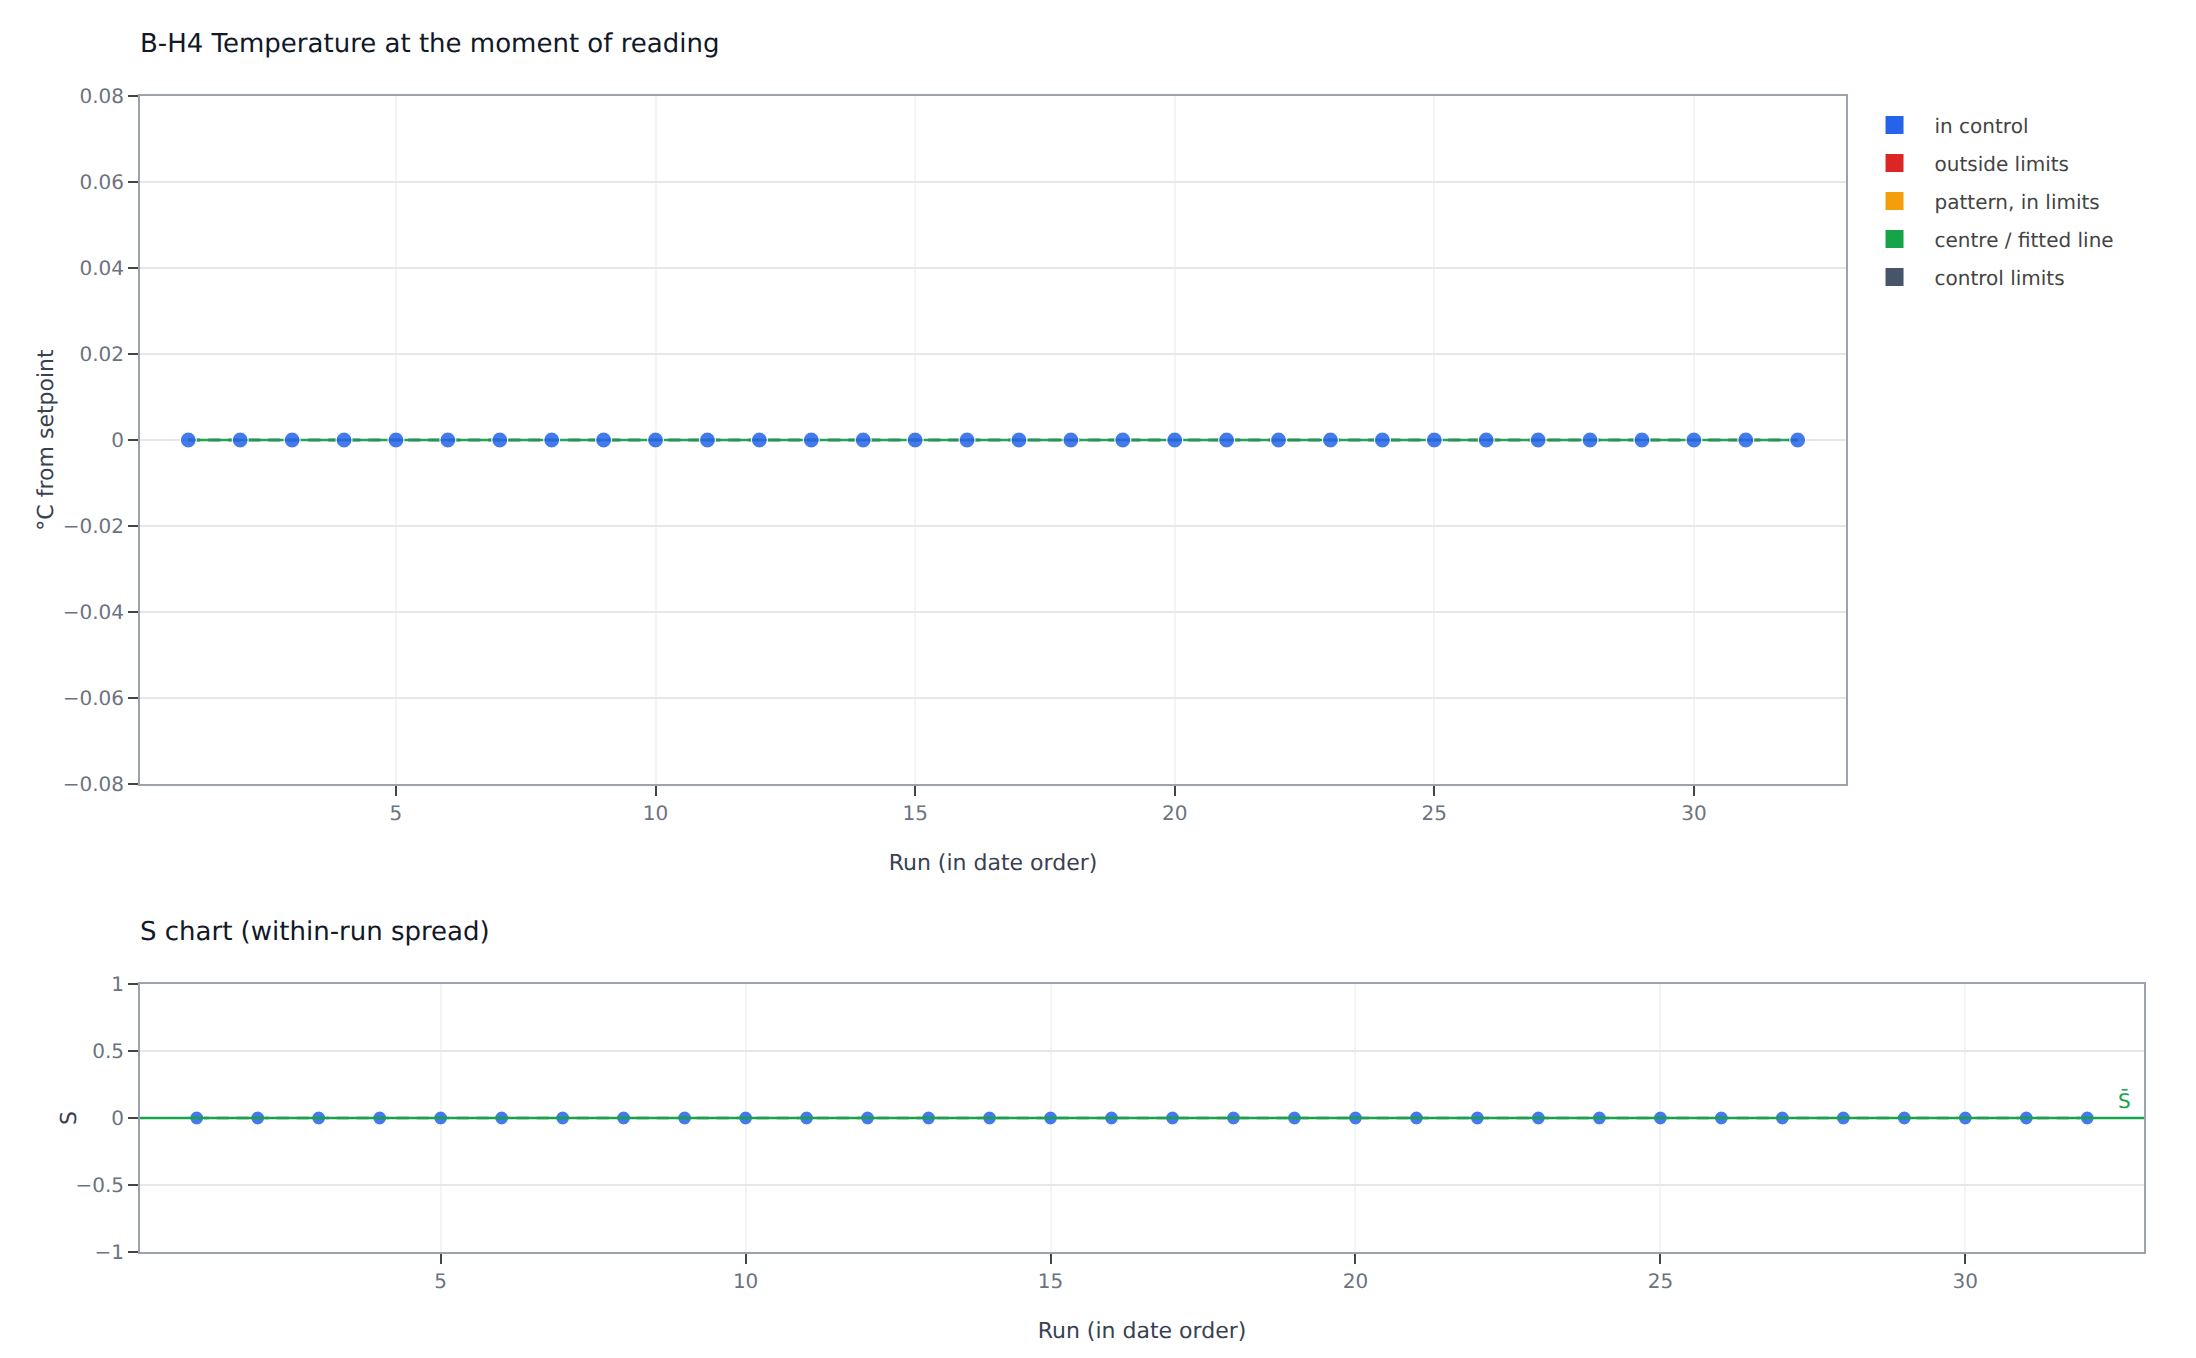
\includegraphics[width=0.92\linewidth,height=0.80\textheight,keepaspectratio]{fig/gallery/cc_type_xbars.png}
\caption[B-H4 Temperature at the moment of reading — xbars chart --- in control]{\synthtag B-H4 Temperature at the moment of reading — xbars chart --- in control. {\footnotesize Exercises \texttt{ccChartSvg}, \texttt{ccCompute}, \texttt{ixMount}, \texttt{renderCcDetail}, \texttt{svgPlot} and 128 more function(s) reachable from them.}}
\label{fig:gal-cc-type-xbars}
\end{figure}

\begin{figure}[H]\centering
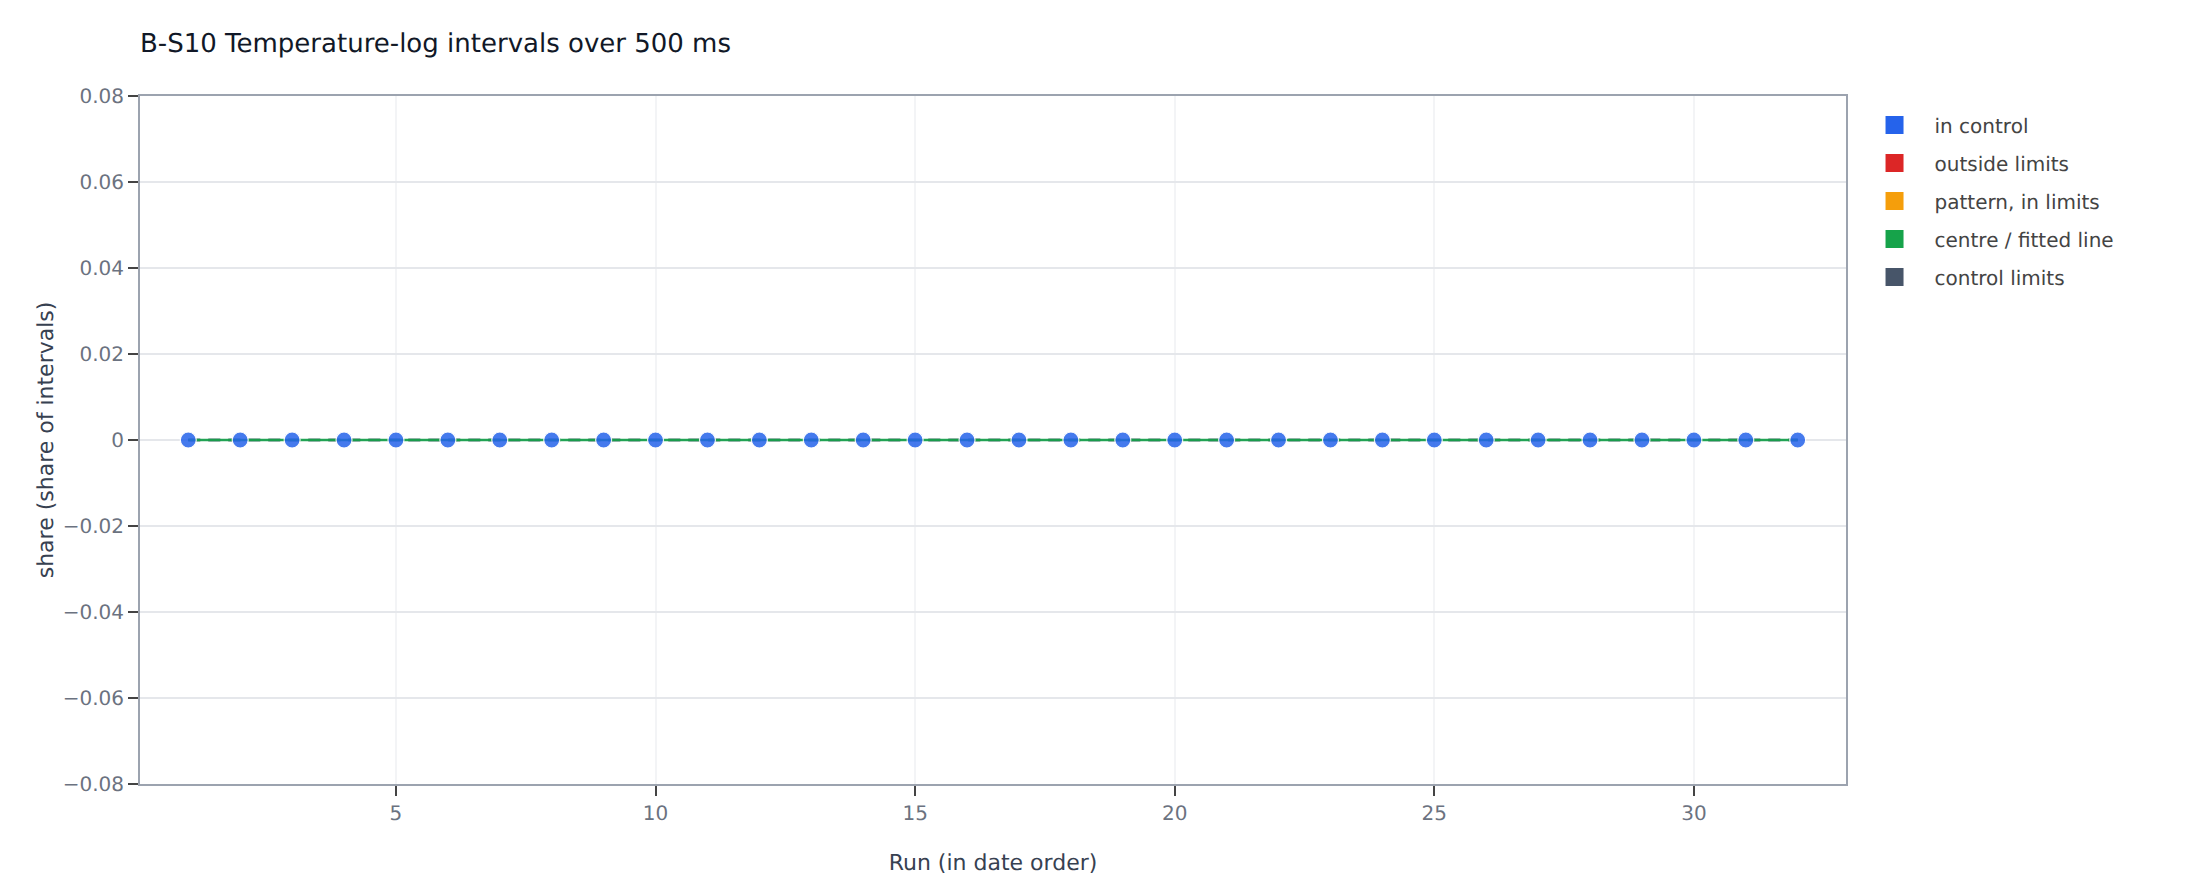
\includegraphics[width=0.92\linewidth,height=0.80\textheight,keepaspectratio]{fig/gallery/cc_type_p.png}
\caption[B-S10 Temperature-log intervals over 500 ms — p chart --- in control]{\synthtag B-S10 Temperature-log intervals over 500 ms — p chart --- in control. {\footnotesize Exercises \texttt{ccChartSvg}, \texttt{ccCompute}, \texttt{ixMount}, \texttt{renderCcDetail}, \texttt{svgPlot} and 128 more function(s) reachable from them.}}
\label{fig:gal-cc-type-p}
\end{figure}

\begin{figure}[H]\centering
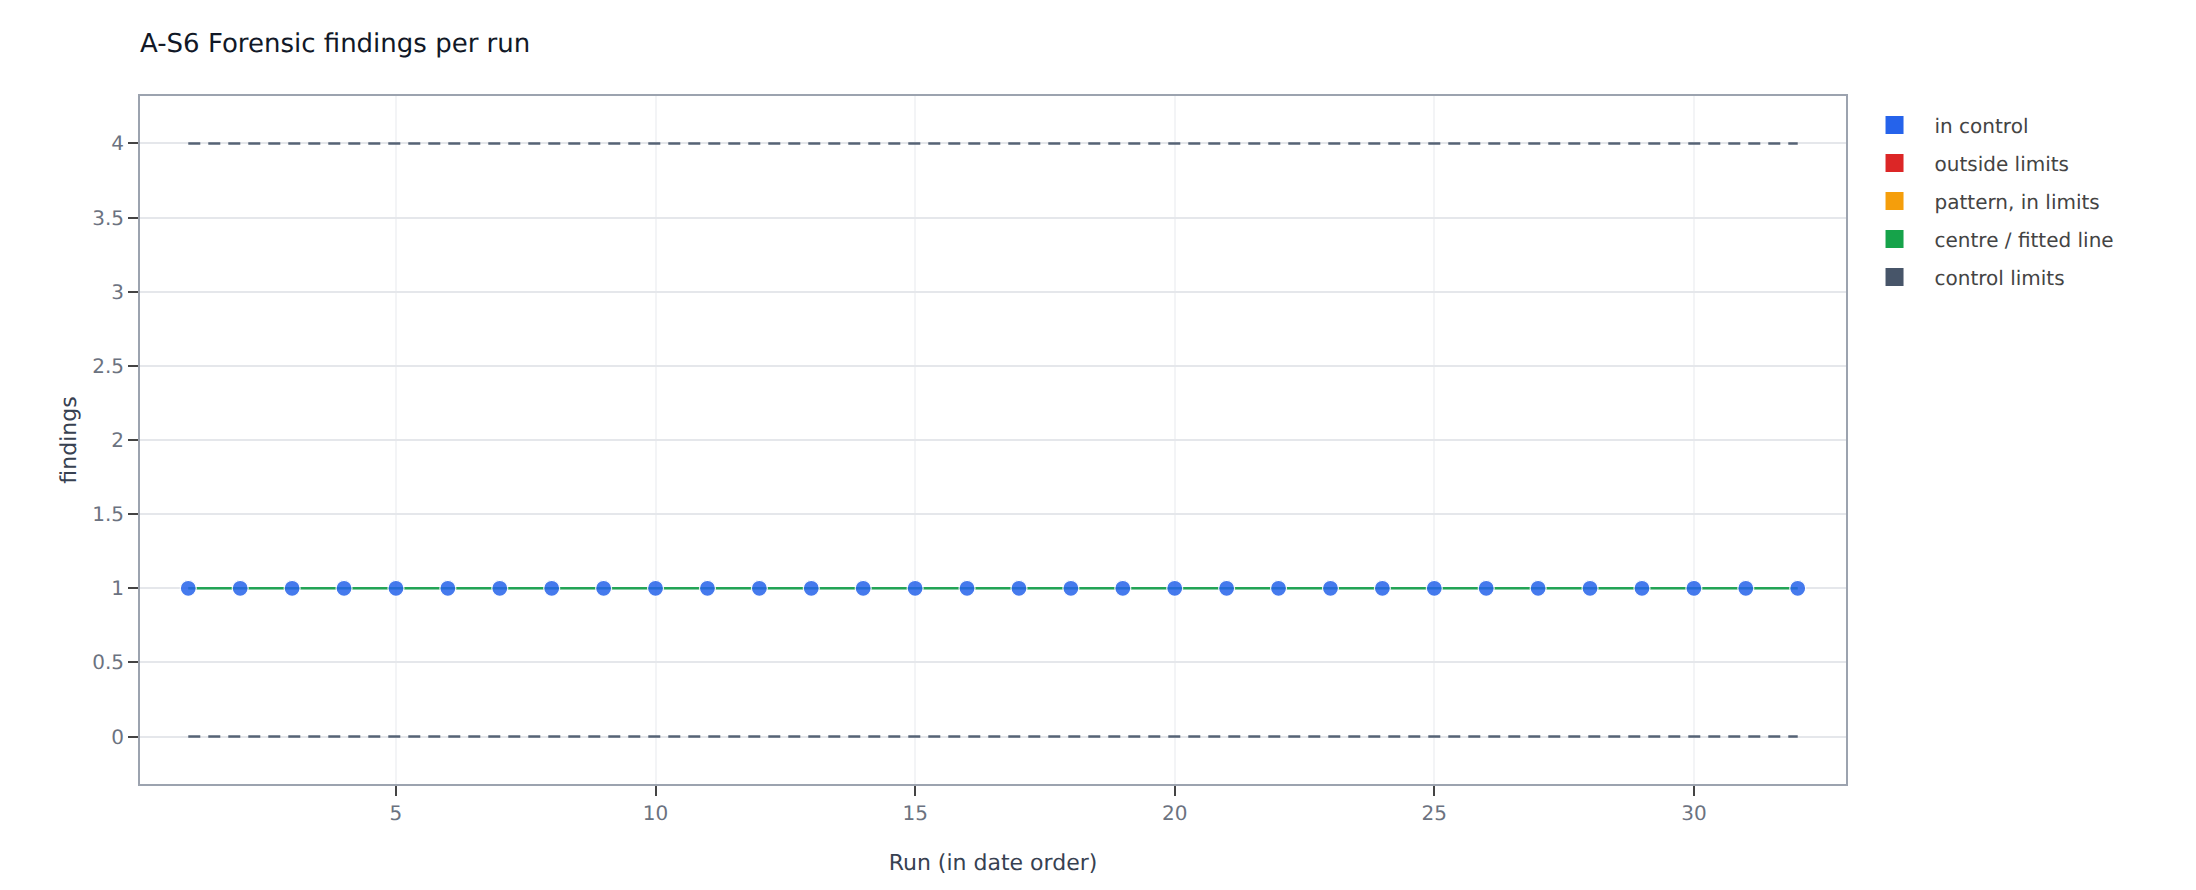
\includegraphics[width=0.92\linewidth,height=0.80\textheight,keepaspectratio]{fig/gallery/cc_type_c.png}
\caption[A-S6 Forensic findings per run — c chart --- in control]{\synthtag A-S6 Forensic findings per run — c chart --- in control. {\footnotesize Exercises \texttt{ccChartSvg}, \texttt{ccCompute}, \texttt{ixMount}, \texttt{renderCcDetail}, \texttt{svgPlot} and 128 more function(s) reachable from them.}}
\label{fig:gal-cc-type-c}
\end{figure}

\begin{figure}[H]\centering
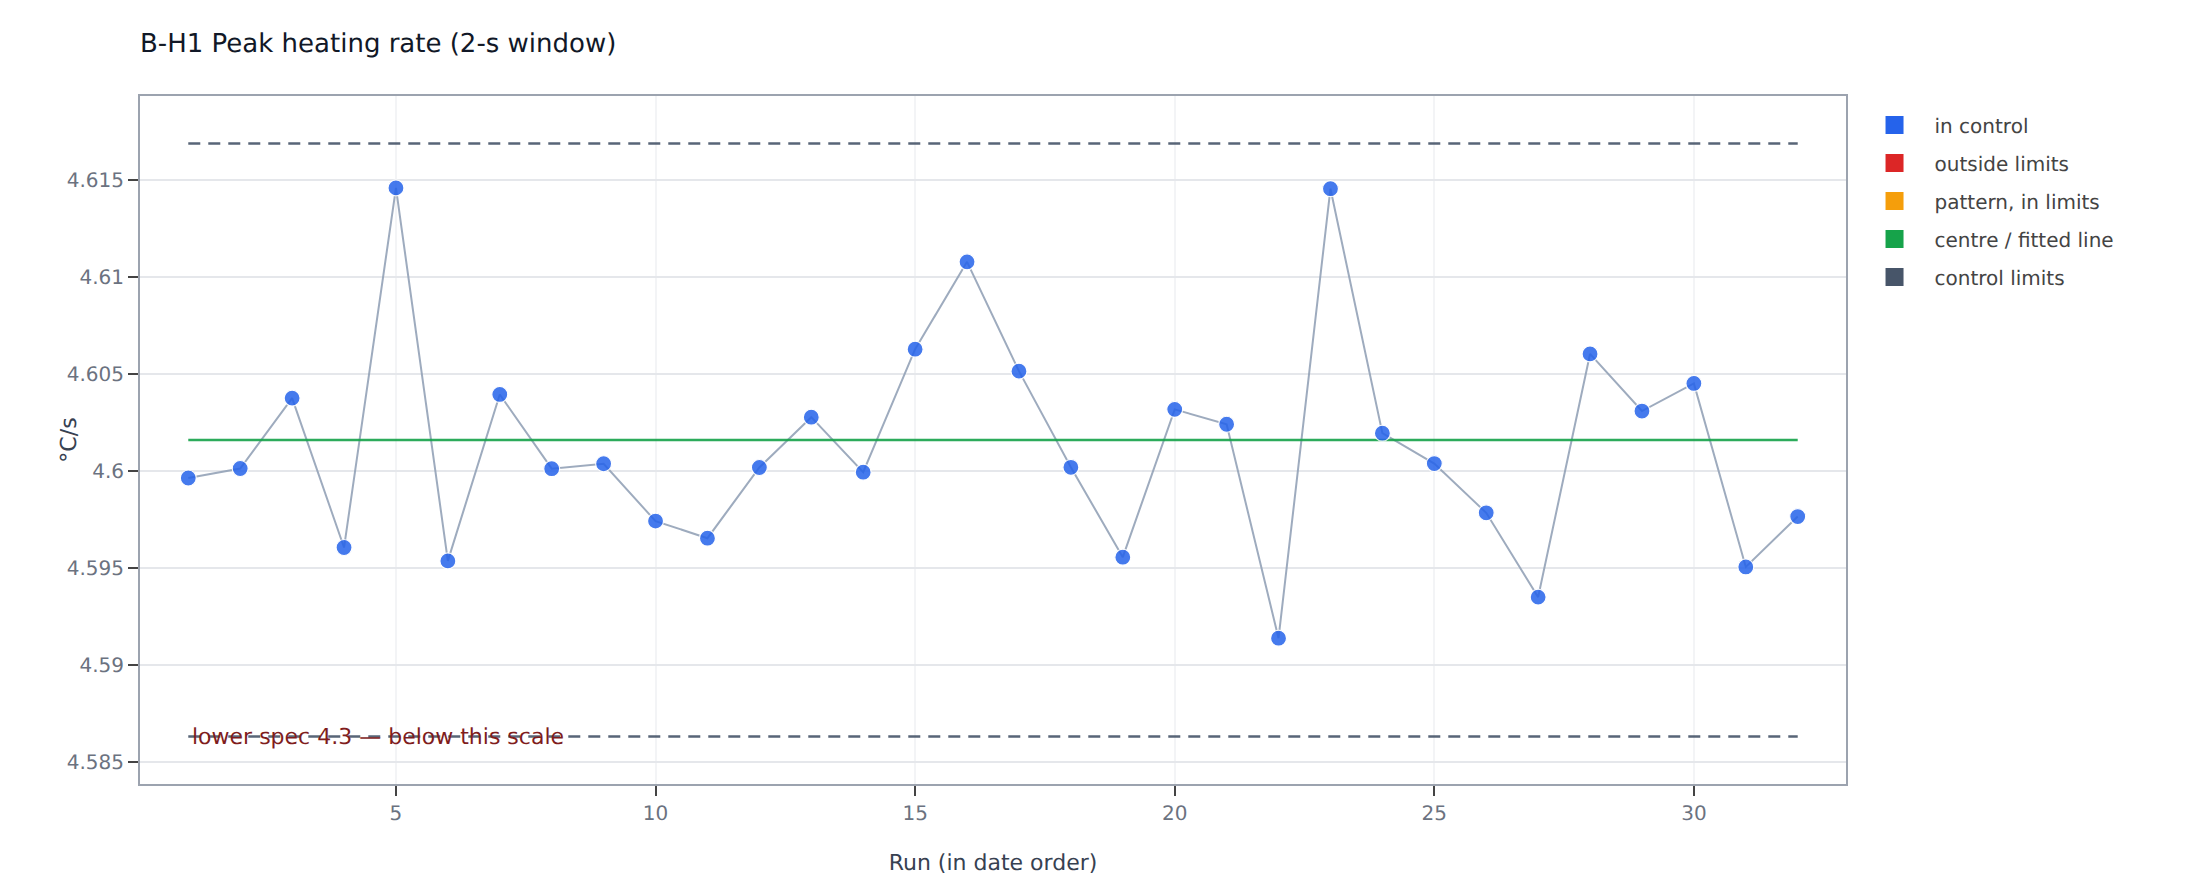
\includegraphics[width=0.92\linewidth,height=0.80\textheight,keepaspectratio]{fig/gallery/cc_in_control_1.png}
\caption[B-H1 Peak heating rate (2-s window) --- in control]{\synthtag B-H1 Peak heating rate (2-s window) --- in control. {\footnotesize Exercises \texttt{ccChartSvg}, \texttt{ccCompute}, \texttt{ccStatus}, \texttt{ccWestgard} and 38 more function(s) reachable from them.}}
\label{fig:gal-cc-in-control-1}
\end{figure}

\begin{figure}[H]\centering
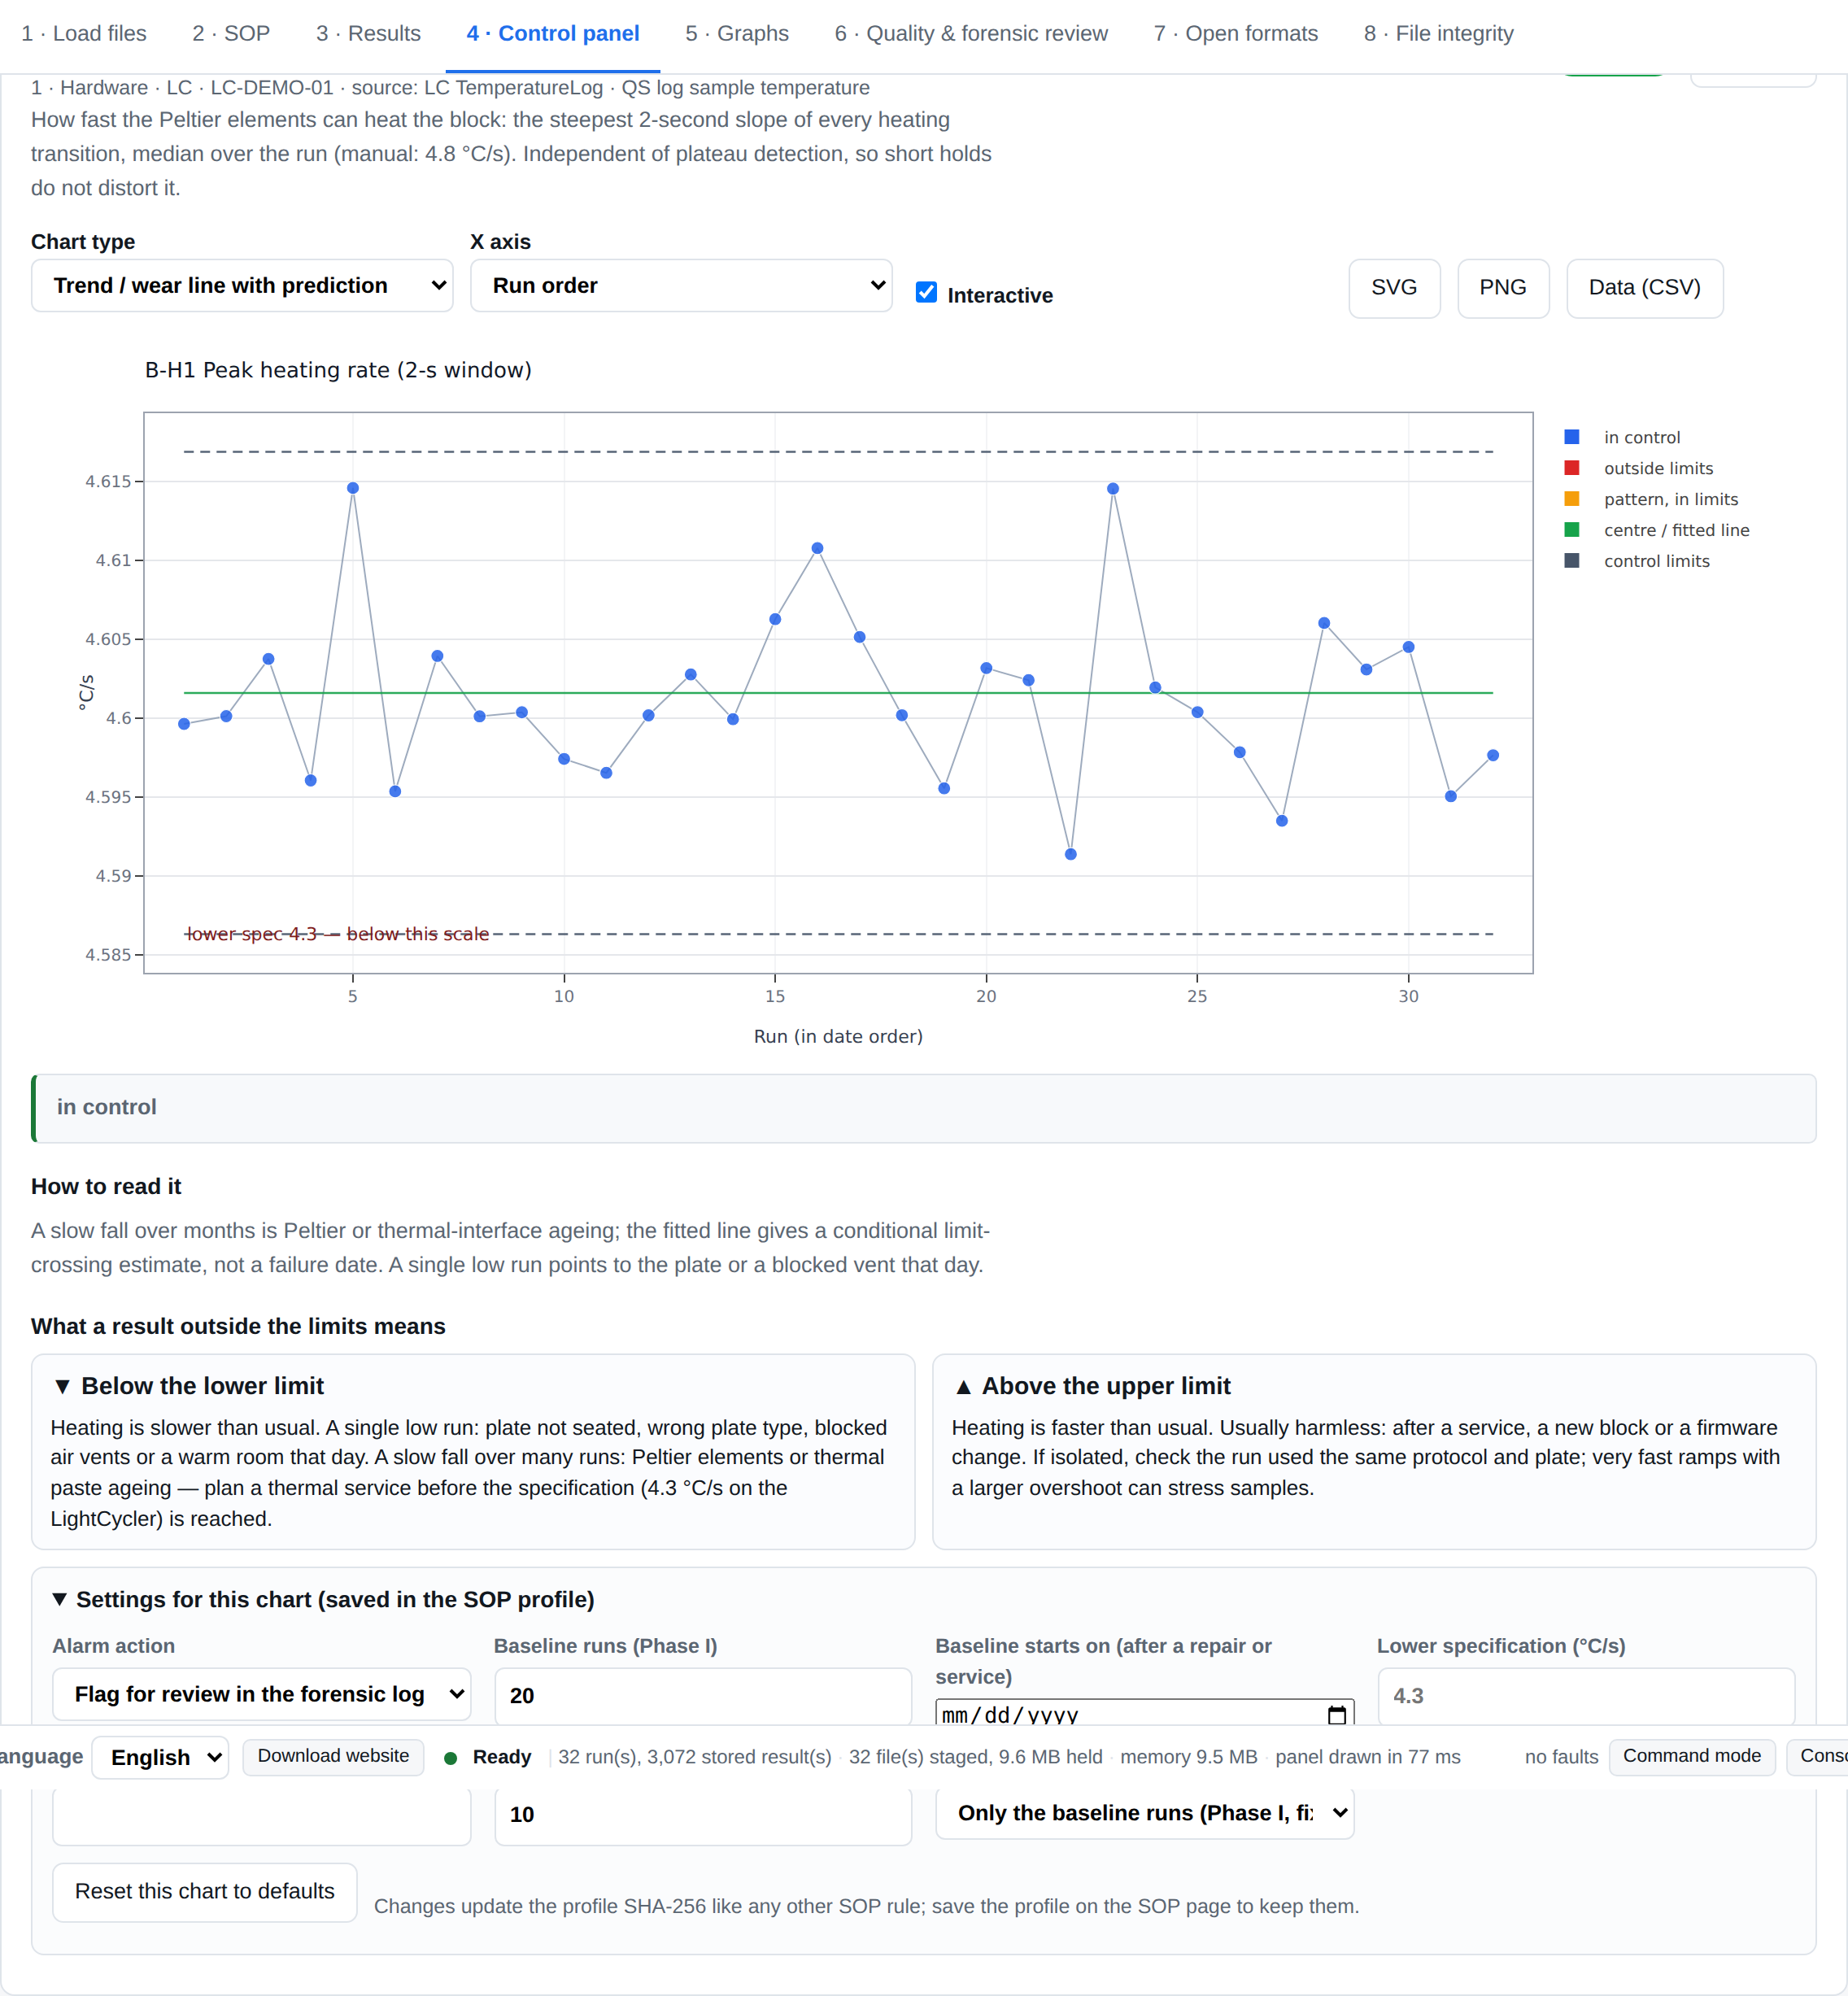
\includegraphics[width=0.92\linewidth,height=0.80\textheight,keepaspectratio]{fig/gallery/cc_in_control_1_card.png}
\caption[The whole record for B-H1 Peak heating rate (2-s window) --- in control]{\synthtag The whole record for B-H1 Peak heating rate (2-s window) --- in control. {\footnotesize Exercises \texttt{ccAlarmDir}, \texttt{ccChartRows}, \texttt{ccStatus}, \texttt{renderCcDetail} and 129 more function(s) reachable from them.}}
\label{fig:gal-cc-in-control-1-card}
\end{figure}

\begin{figure}[H]\centering
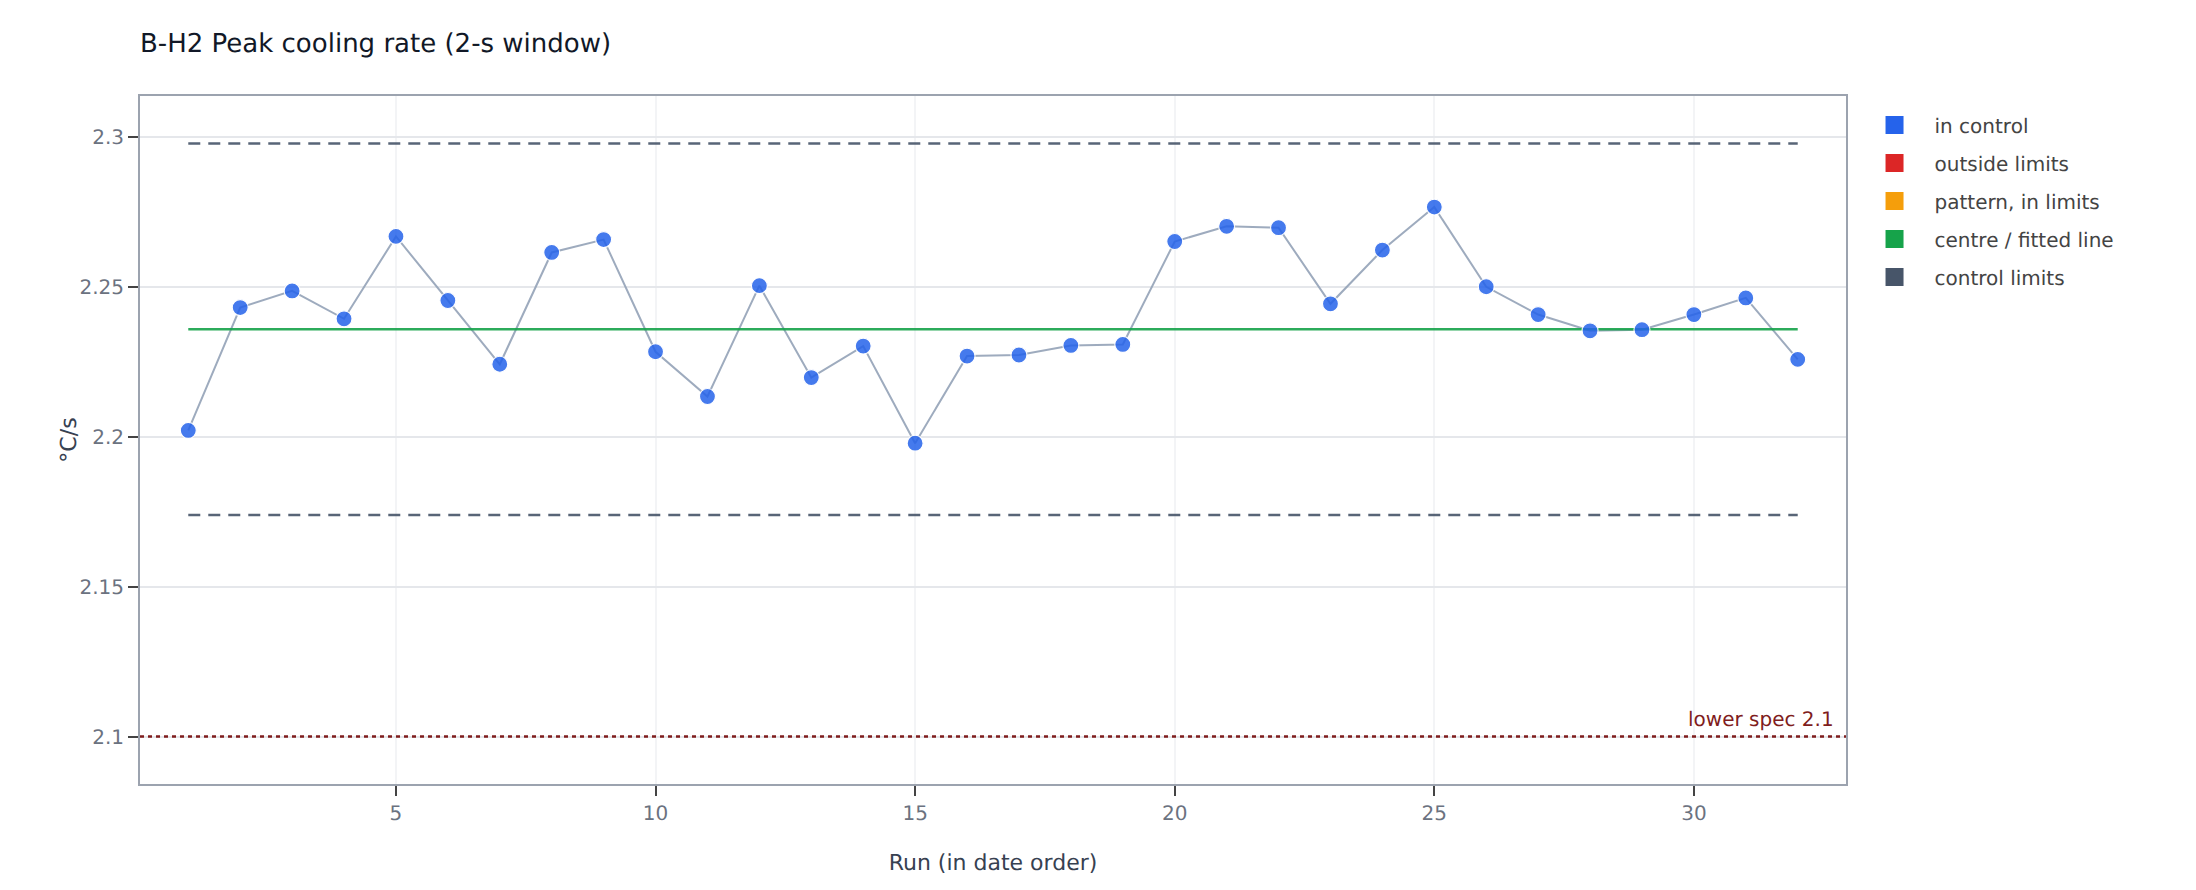
\includegraphics[width=0.92\linewidth,height=0.80\textheight,keepaspectratio]{fig/gallery/cc_in_control_2.png}
\caption[B-H2 Peak cooling rate (2-s window) --- in control]{\synthtag B-H2 Peak cooling rate (2-s window) --- in control. {\footnotesize Exercises \texttt{ccChartSvg}, \texttt{ccCompute}, \texttt{ccStatus}, \texttt{ccWestgard} and 38 more function(s) reachable from them.}}
\label{fig:gal-cc-in-control-2}
\end{figure}

\begin{figure}[H]\centering
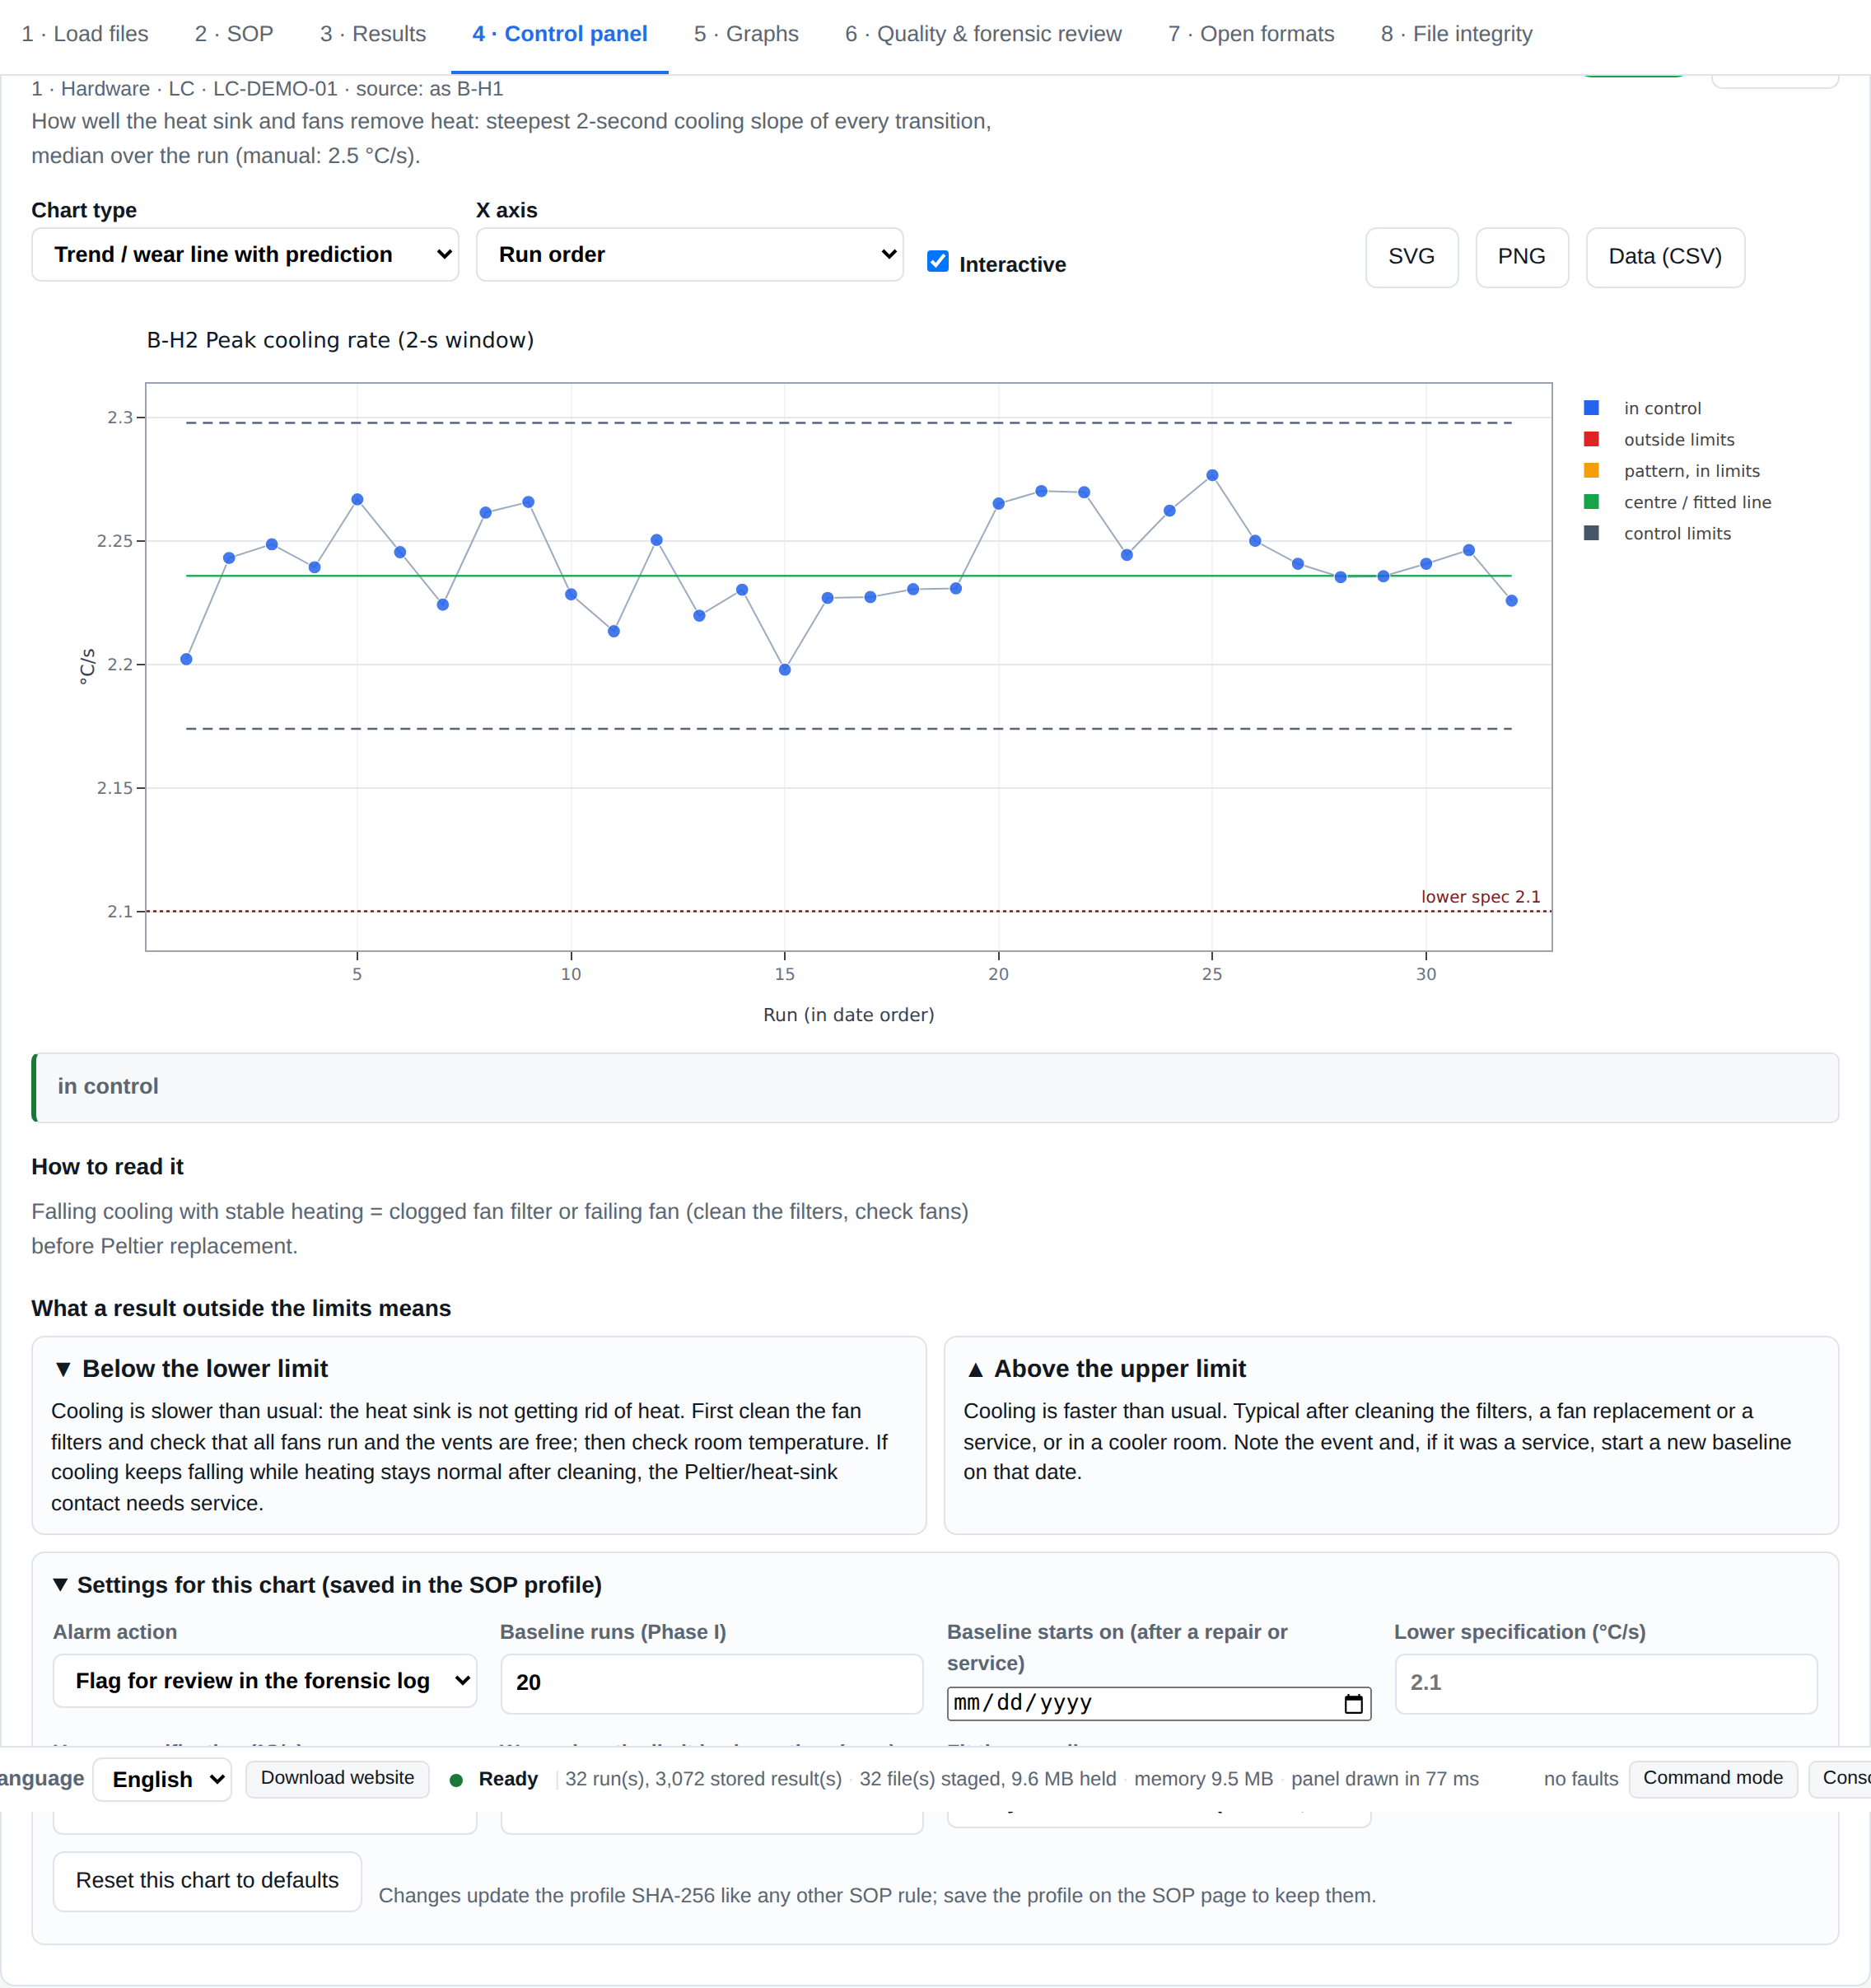
\includegraphics[width=0.92\linewidth,height=0.80\textheight,keepaspectratio]{fig/gallery/cc_in_control_2_card.png}
\caption[The whole record for B-H2 Peak cooling rate (2-s window) --- in control]{\synthtag The whole record for B-H2 Peak cooling rate (2-s window) --- in control. {\footnotesize Exercises \texttt{ccAlarmDir}, \texttt{ccChartRows}, \texttt{ccStatus}, \texttt{renderCcDetail} and 129 more function(s) reachable from them.}}
\label{fig:gal-cc-in-control-2-card}
\end{figure}

\begin{figure}[H]\centering
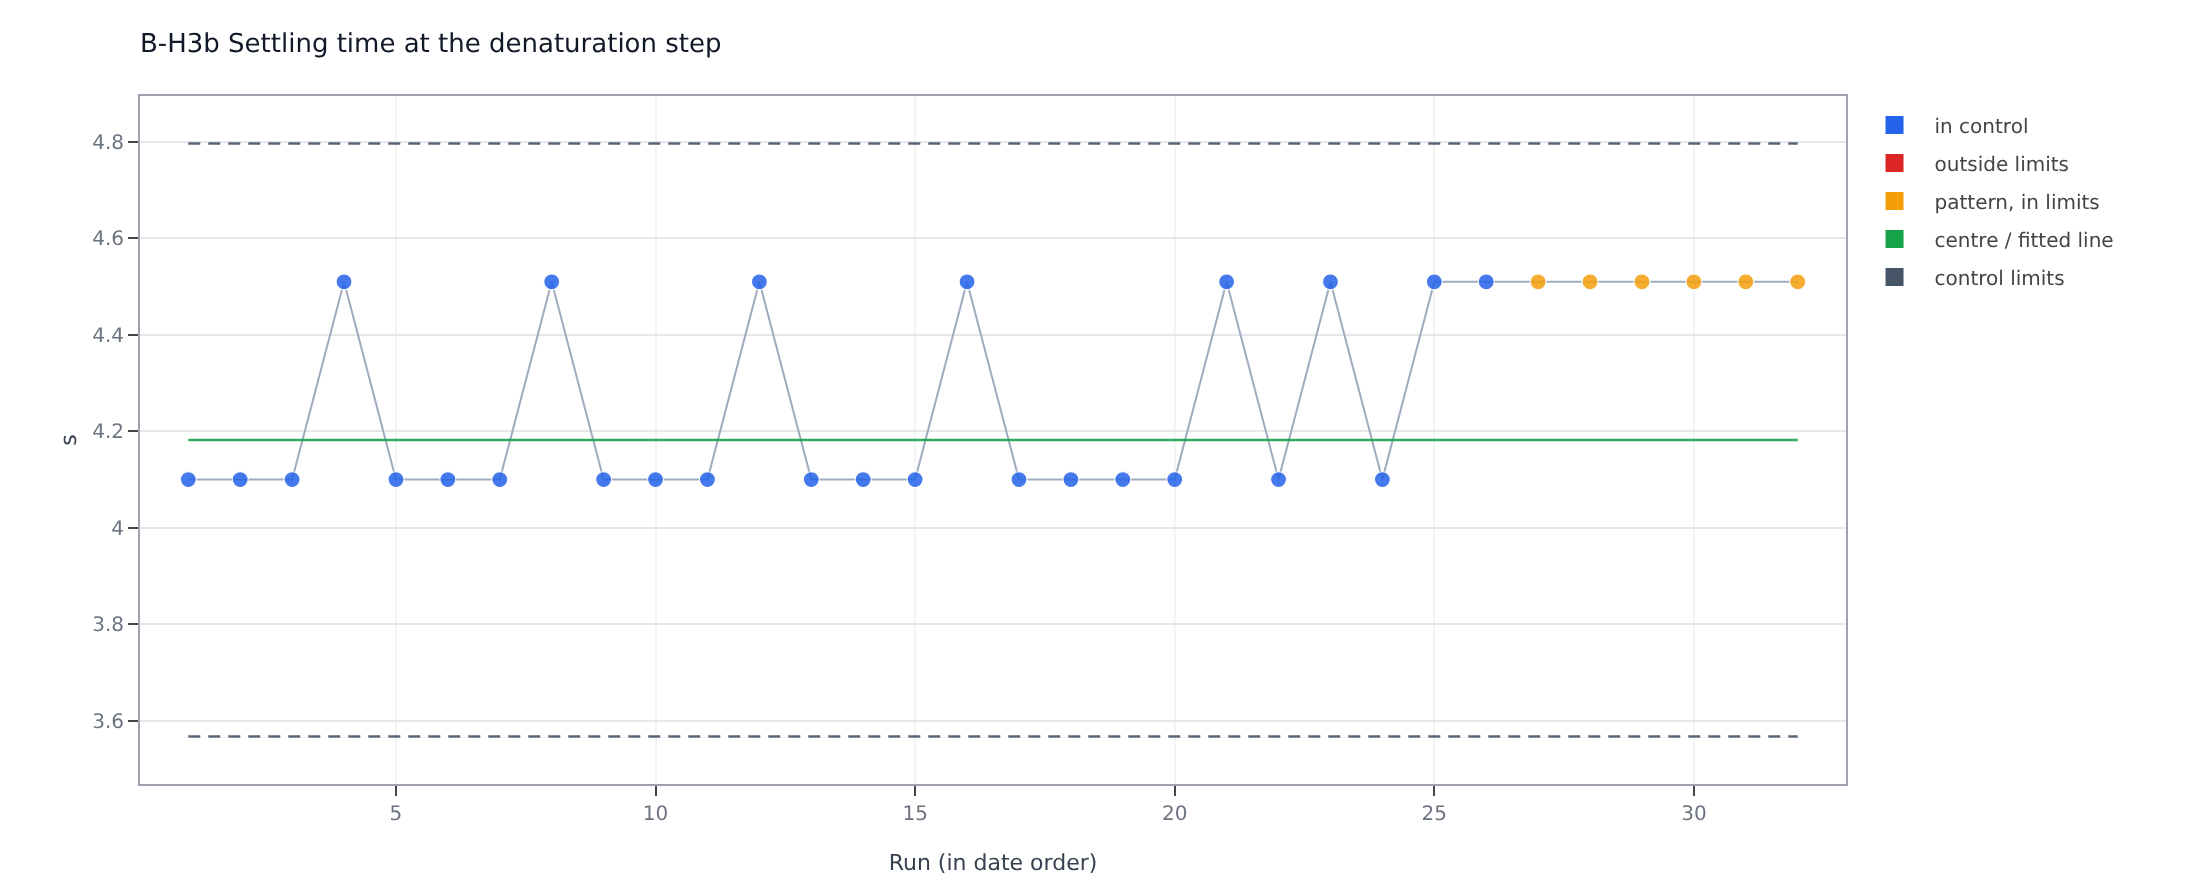
\includegraphics[width=0.92\linewidth,height=0.80\textheight,keepaspectratio]{fig/gallery/cc_alarm_1.png}
\caption[B-H3b Settling time at the denaturation step --- pattern inside the limits: 4 of 5 beyond 1σ, 8 on one side]{\synthtag B-H3b Settling time at the denaturation step --- pattern inside the limits: 4 of 5 beyond 1σ, 8 on one side. {\footnotesize Exercises \texttt{ccChartSvg}, \texttt{ccCompute}, \texttt{ccStatus}, \texttt{ccWestgard} and 38 more function(s) reachable from them.}}
\label{fig:gal-cc-alarm-1}
\end{figure}

\begin{figure}[H]\centering
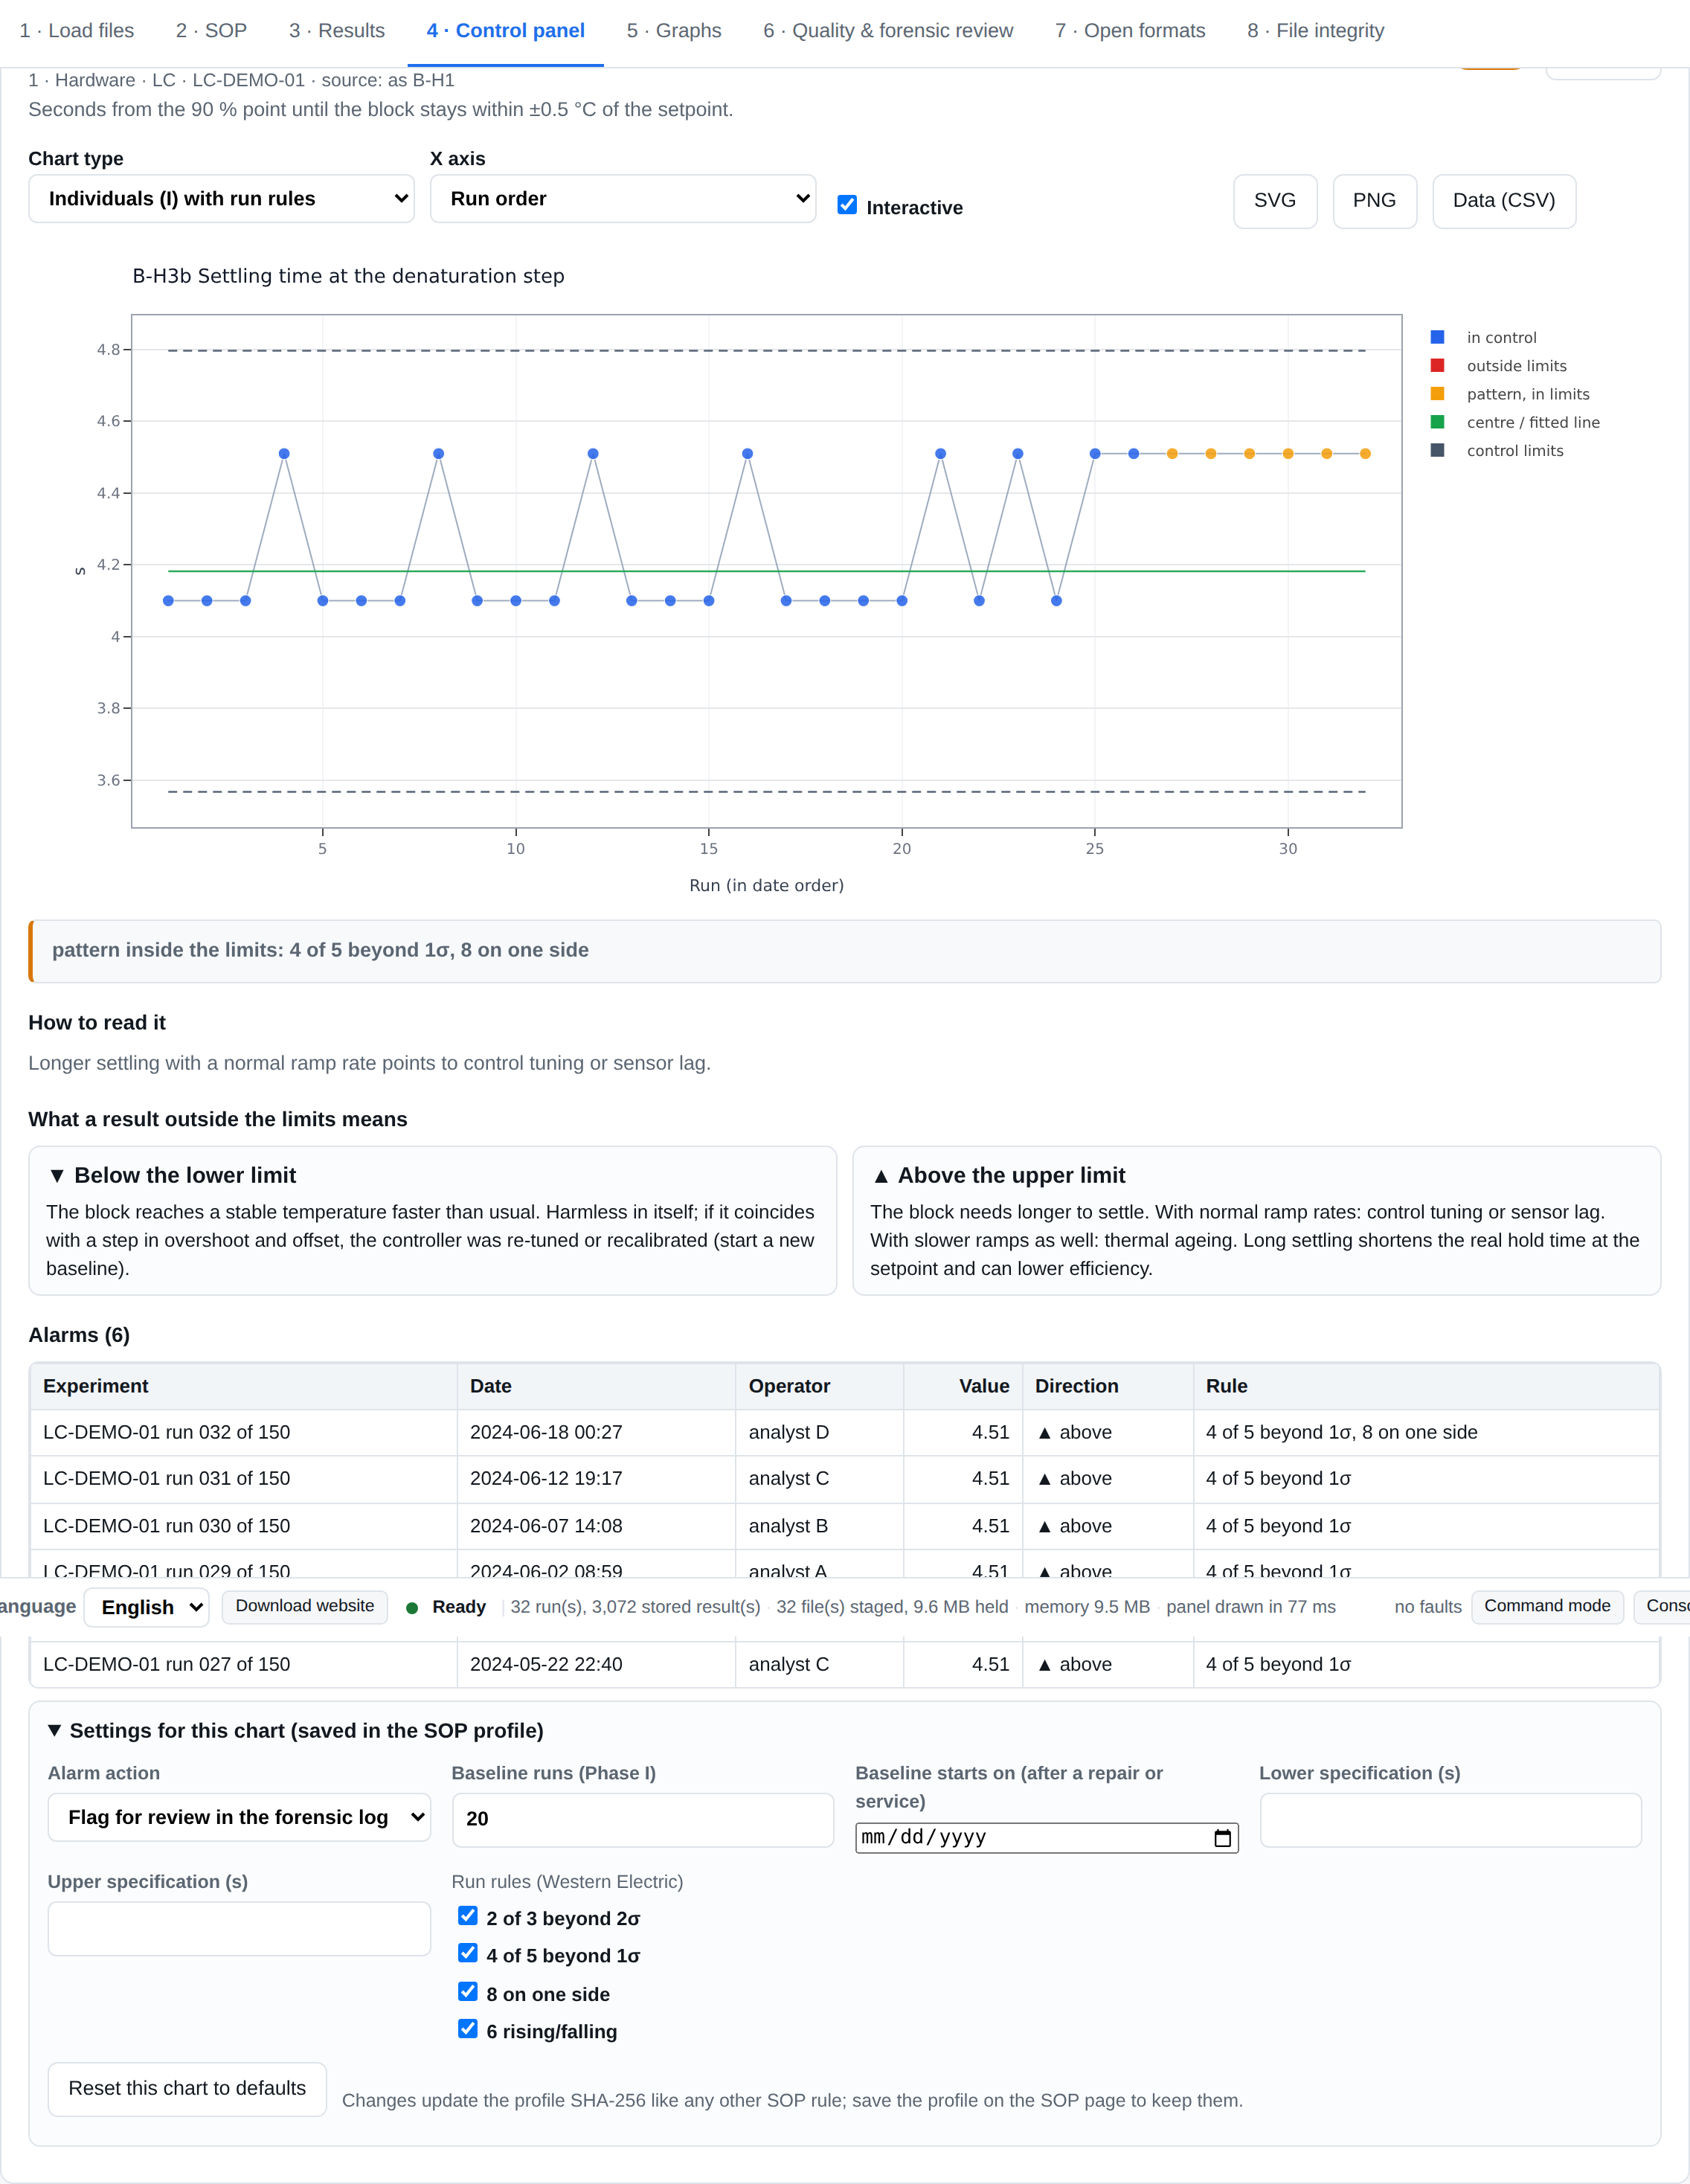
\includegraphics[width=0.92\linewidth,height=0.80\textheight,keepaspectratio]{fig/gallery/cc_alarm_1_card.png}
\caption[The whole record for B-H3b Settling time at the denaturation step --- pattern inside the limits: 4 of 5 beyond 1σ, 8 on one side]{\synthtag The whole record for B-H3b Settling time at the denaturation step --- pattern inside the limits: 4 of 5 beyond 1σ, 8 on one side. {\footnotesize Exercises \texttt{ccAlarmDir}, \texttt{ccChartRows}, \texttt{ccStatus}, \texttt{renderCcDetail} and 129 more function(s) reachable from them.}}
\label{fig:gal-cc-alarm-1-card}
\end{figure}

\section{The same page out of control}
Scenario S9: a calibrator lot changes at run~9. The control steps from about 24.2 to about 24.6 and drifts to 24.9 by run~20 while efficiency stays stable. Nothing in the page was configured differently; only the files changed.

\begin{figure}[H]\centering
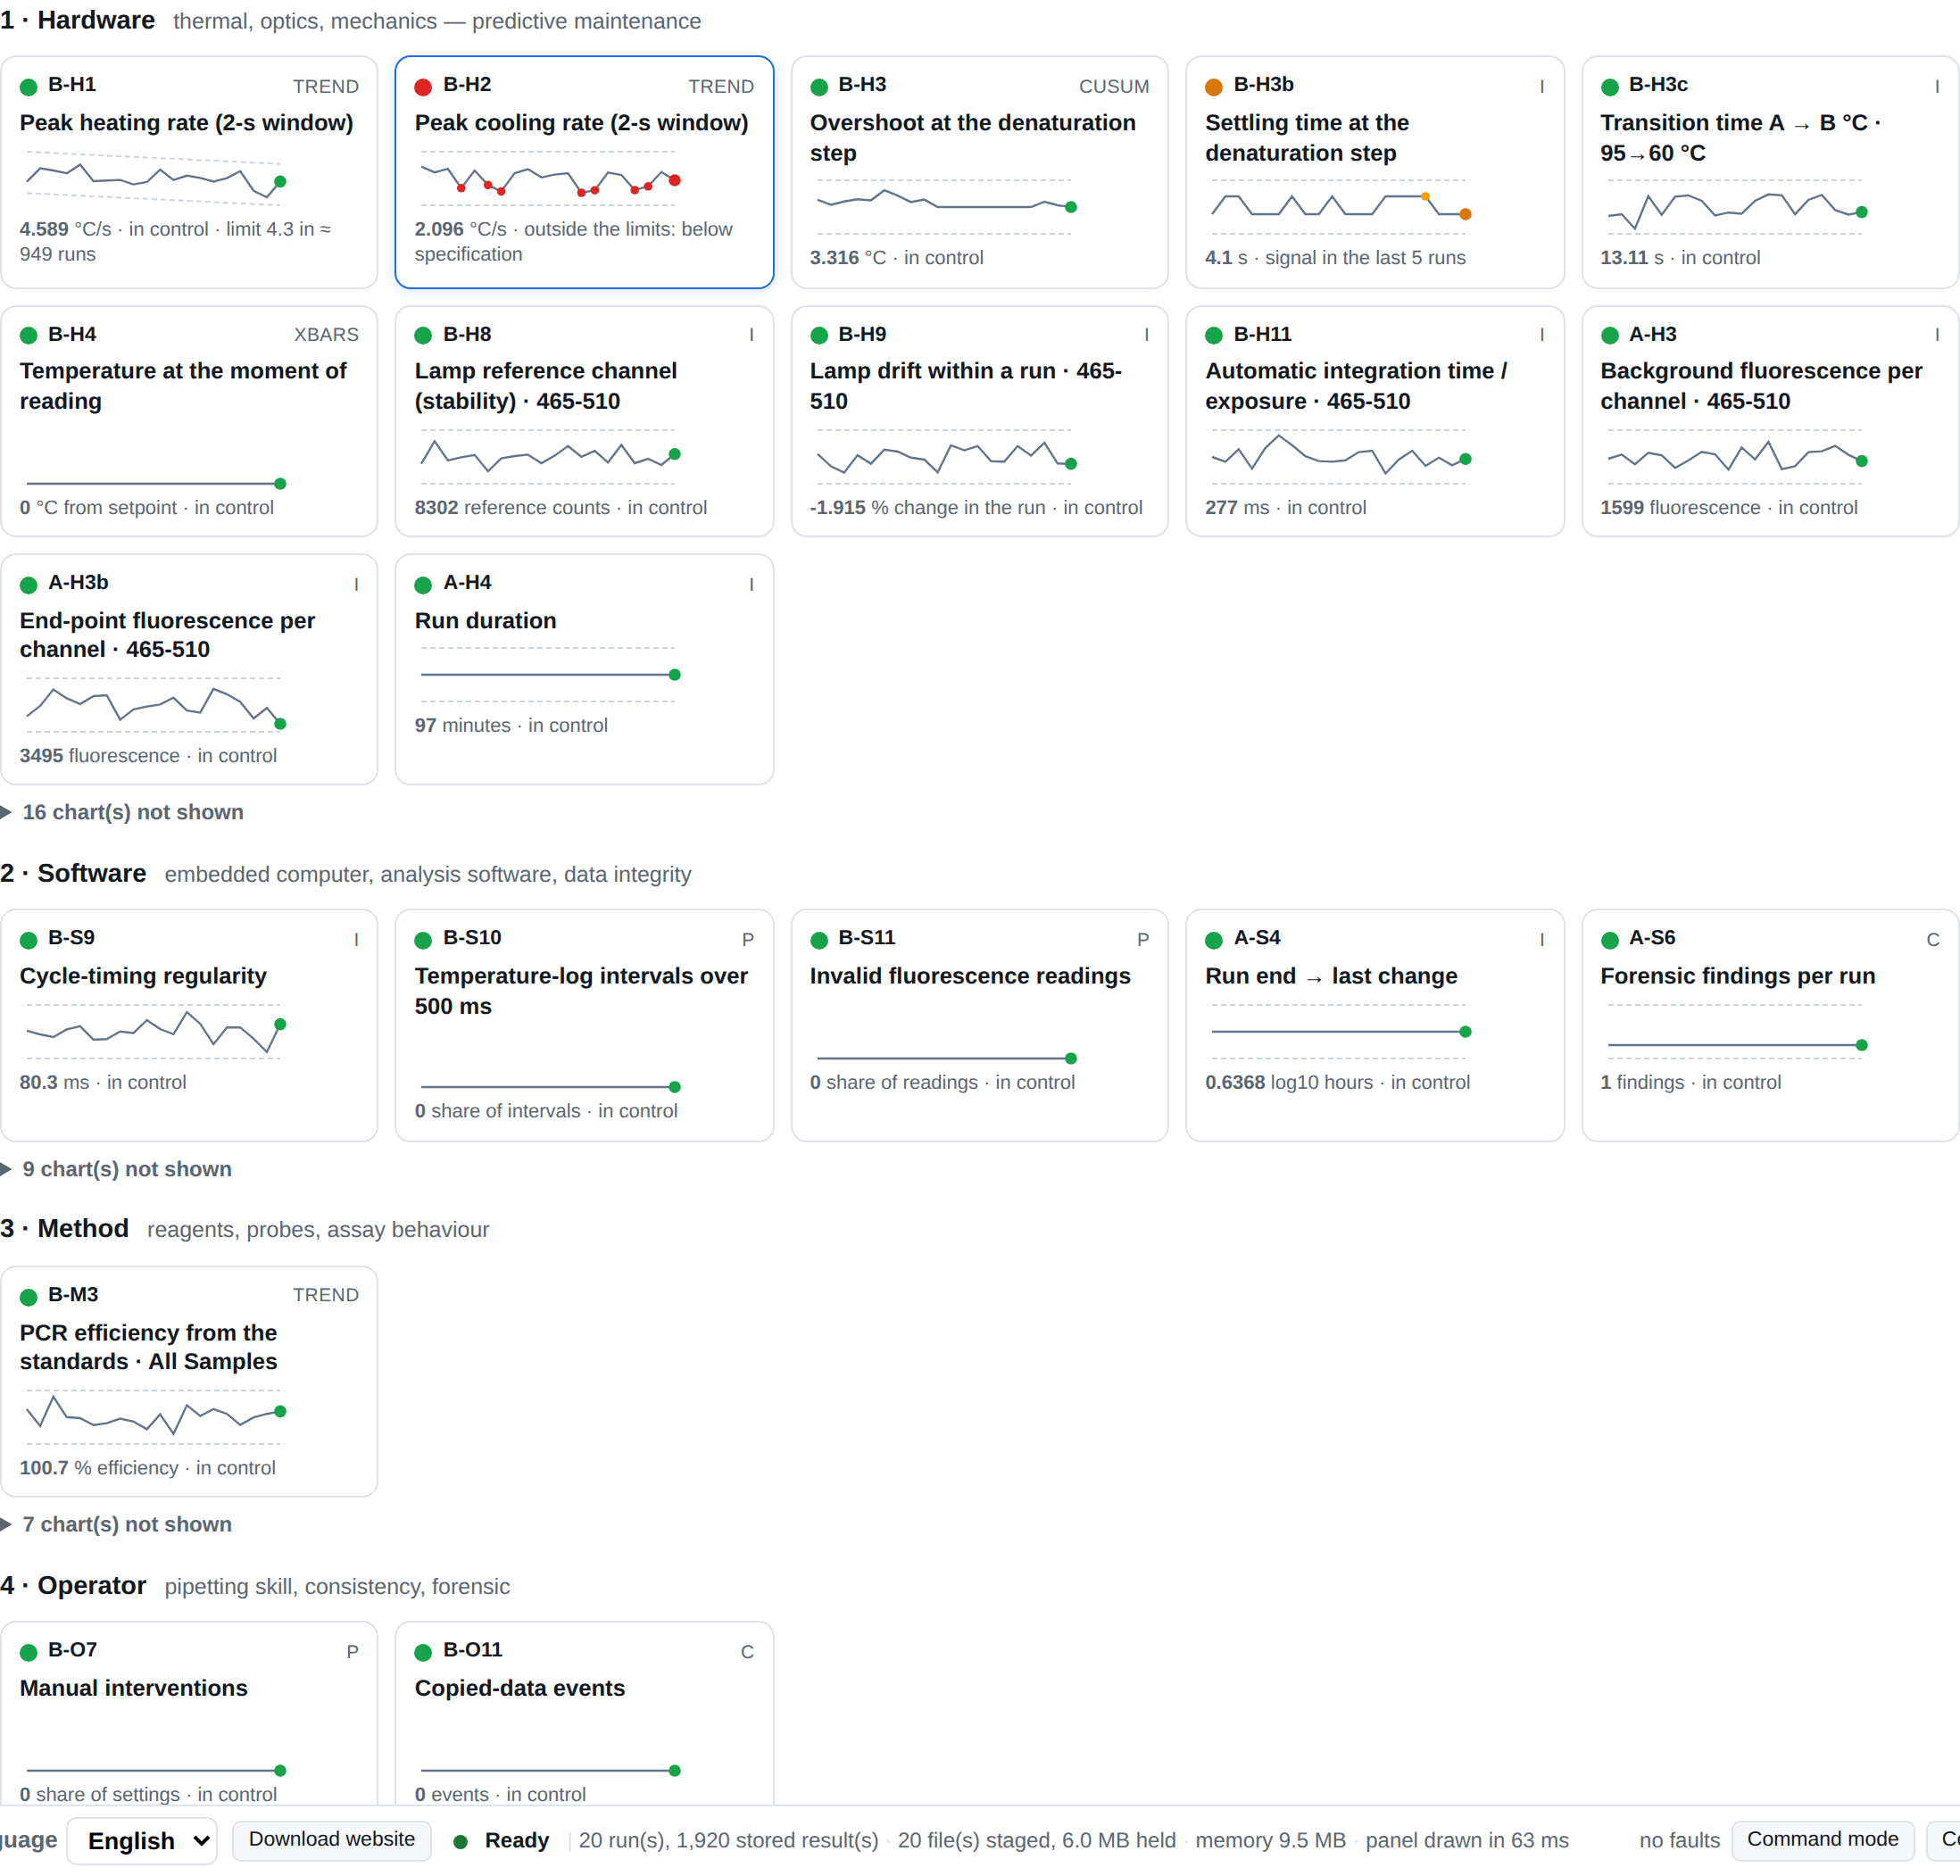
\includegraphics[width=0.98\linewidth,height=0.80\textheight,keepaspectratio]{fig/gallery/s9_overview.png}
\caption[Control panel on the planted step change (scenario S9) --- the control steps at run 9 and drifts afterwards]{\synthtag Control panel on the planted step change (scenario S9) --- the control steps at run 9 and drifts afterwards. {\footnotesize Exercises \texttt{ccCompute}, \texttt{ccStatus}, \texttt{renderPanel} and 130 more function(s) reachable from them.}}
\label{fig:gal-s9-overview}
\end{figure}

\begin{figure}[H]\centering
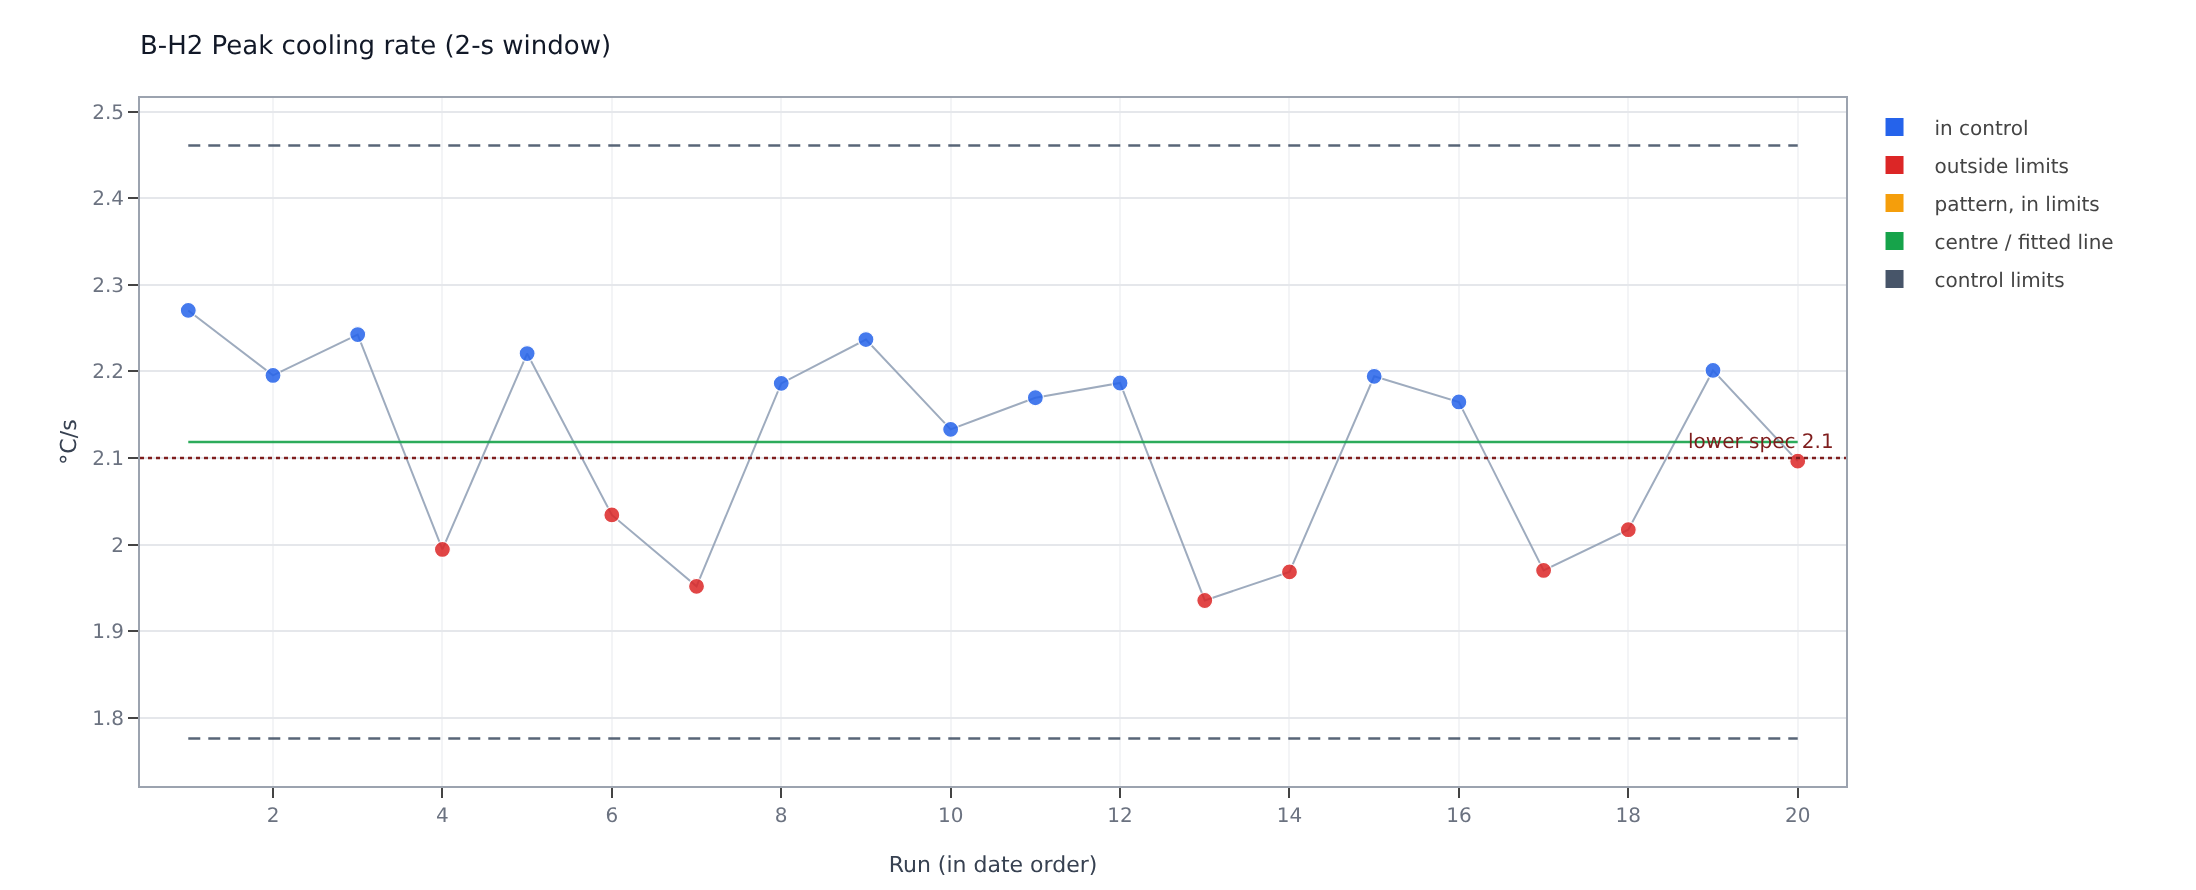
\includegraphics[width=0.92\linewidth,height=0.80\textheight,keepaspectratio]{fig/gallery/s9_alarm_1.png}
\caption[B-H2 Peak cooling rate (2-s window) — out of control --- 8 flagged point(s): outside the limits: below specification]{\synthtag B-H2 Peak cooling rate (2-s window) — out of control --- 8 flagged point(s): outside the limits: below specification. {\footnotesize Exercises \texttt{ccChartSvg}, \texttt{ccCompute}, \texttt{ccStatus}, \texttt{ccWestgard} and 38 more function(s) reachable from them.}}
\label{fig:gal-s9-alarm-1}
\end{figure}

\begin{figure}[H]\centering
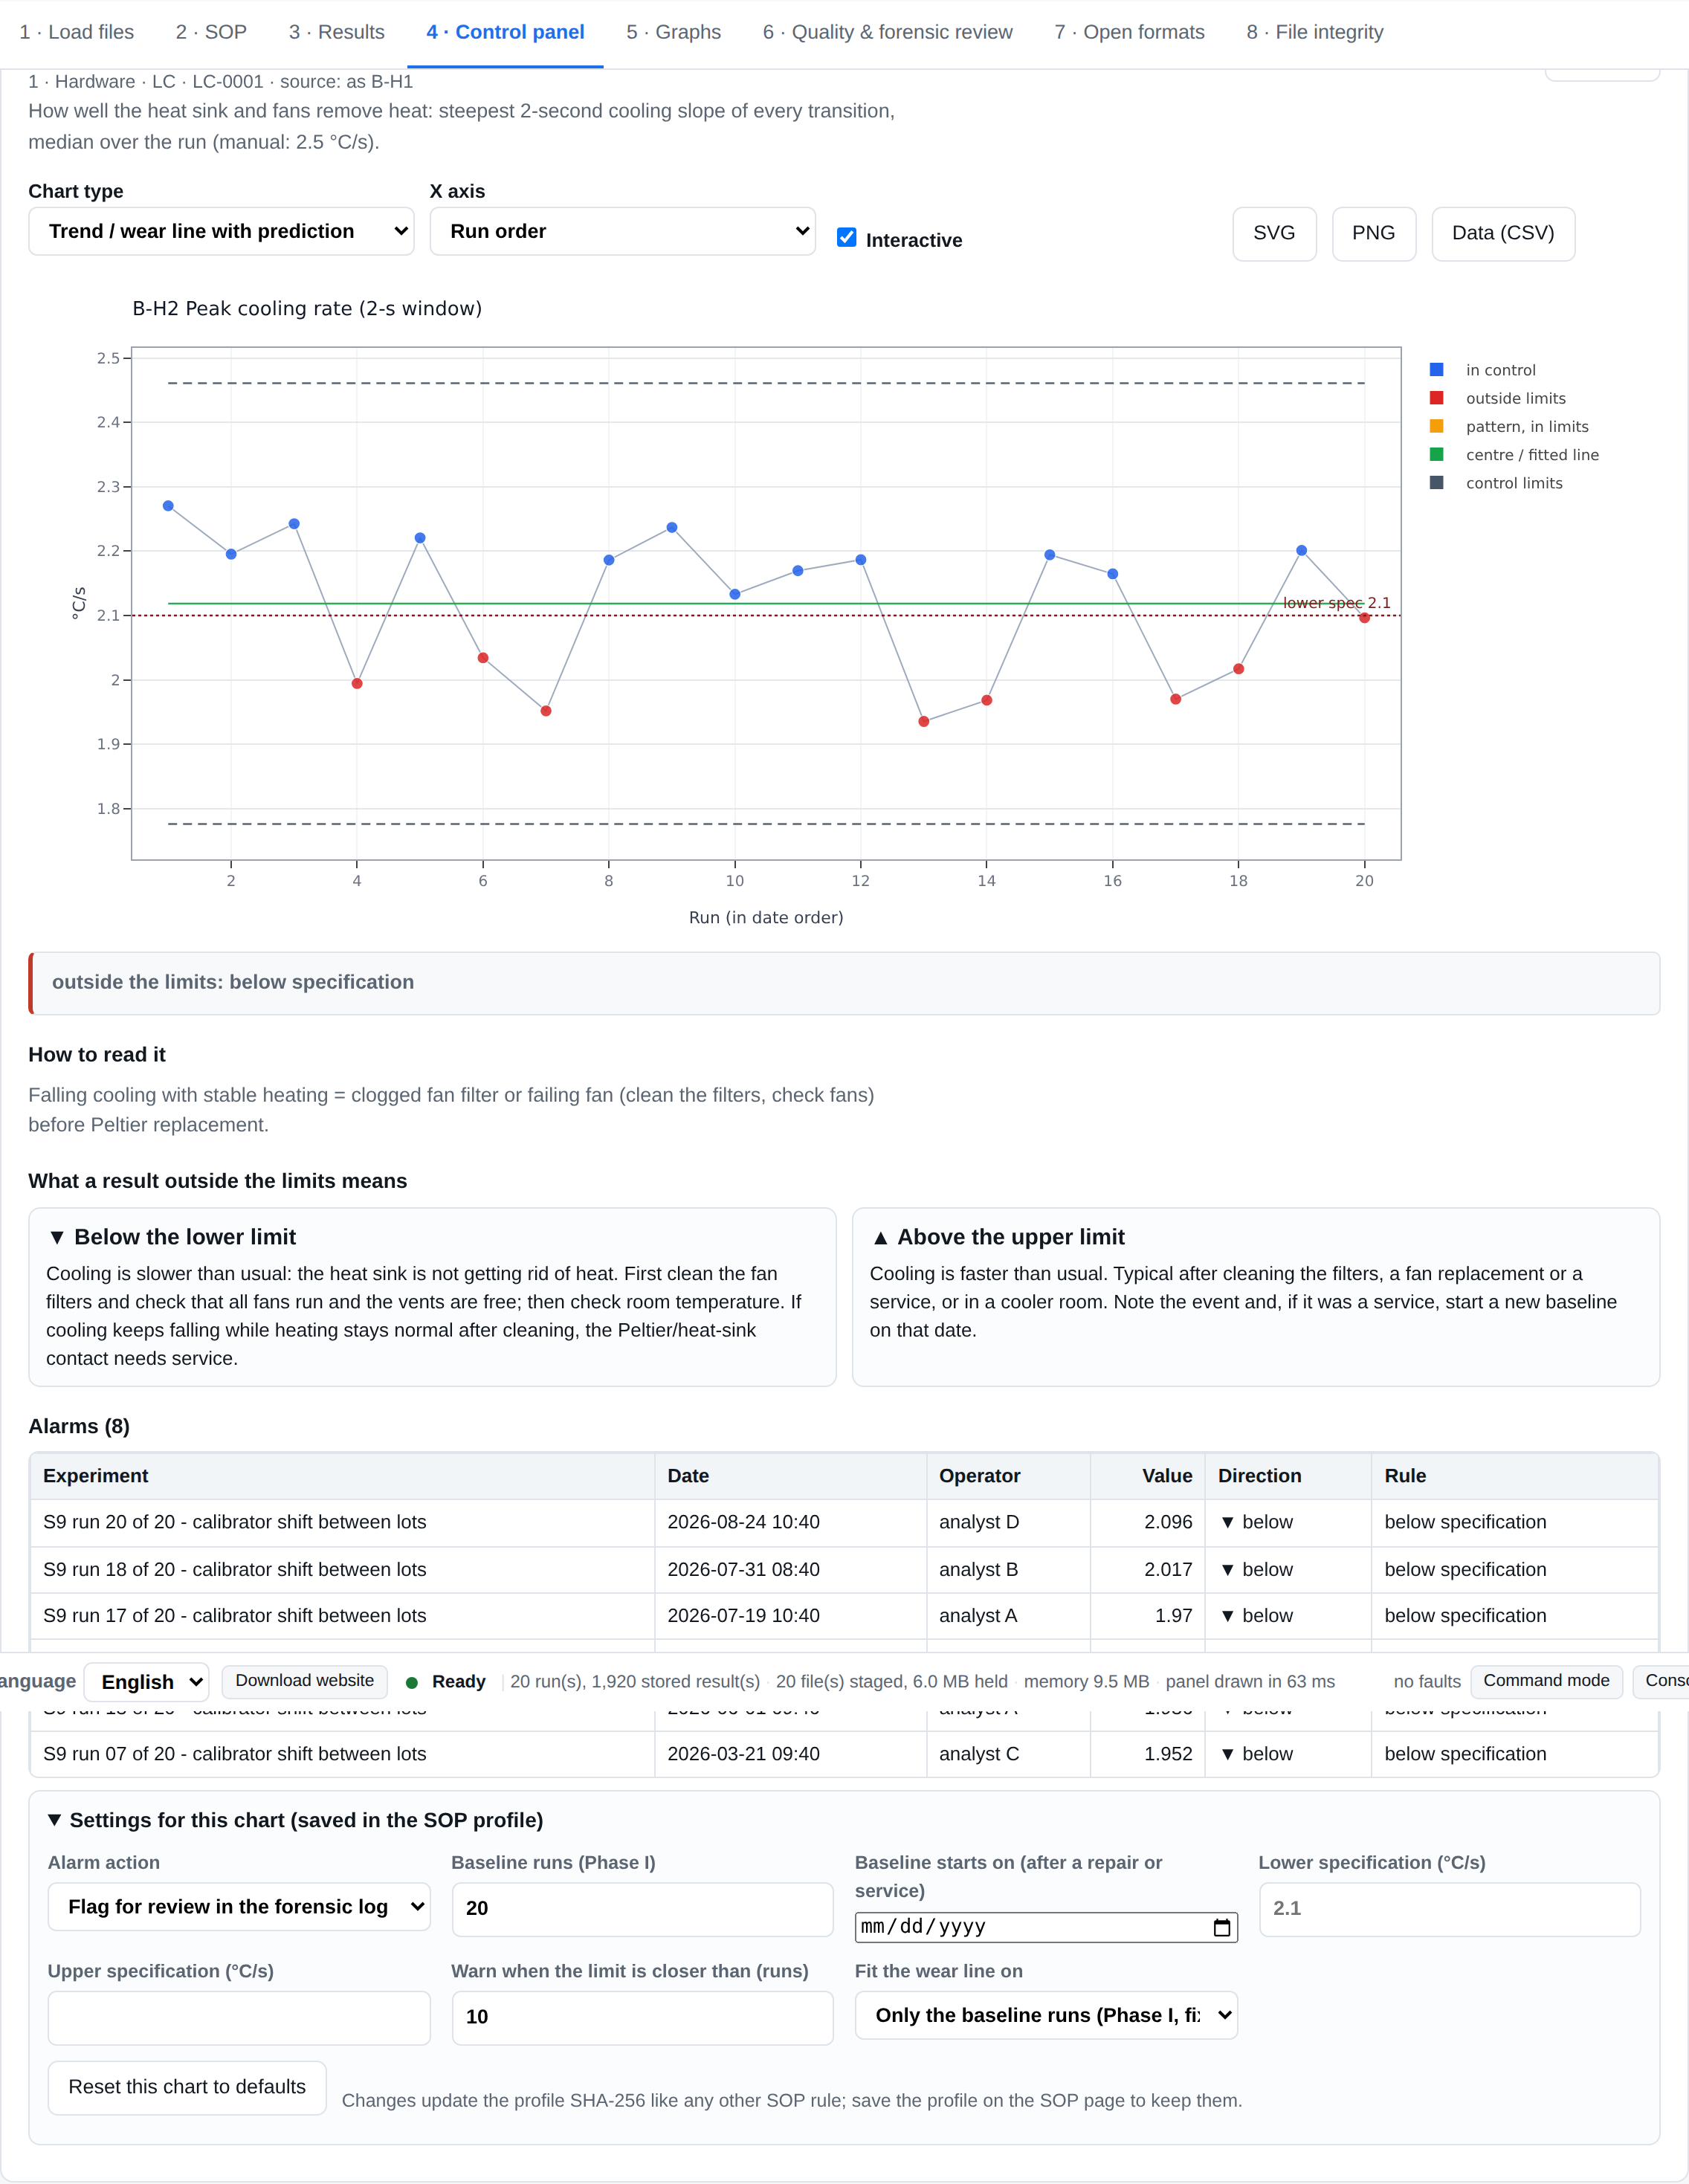
\includegraphics[width=0.92\linewidth,height=0.80\textheight,keepaspectratio]{fig/gallery/s9_alarm_1_card.png}
\caption[The alarm record for B-H2 Peak cooling rate (2-s window) --- outside the limits: below specification]{\synthtag The alarm record for B-H2 Peak cooling rate (2-s window) --- outside the limits: below specification. {\footnotesize Exercises \texttt{ccAlarmDir}, \texttt{ccChartRows}, \texttt{ccStatus}, \texttt{renderCcDetail} and 129 more function(s) reachable from them.}}
\label{fig:gal-s9-alarm-1-card}
\end{figure}

\begin{figure}[H]\centering
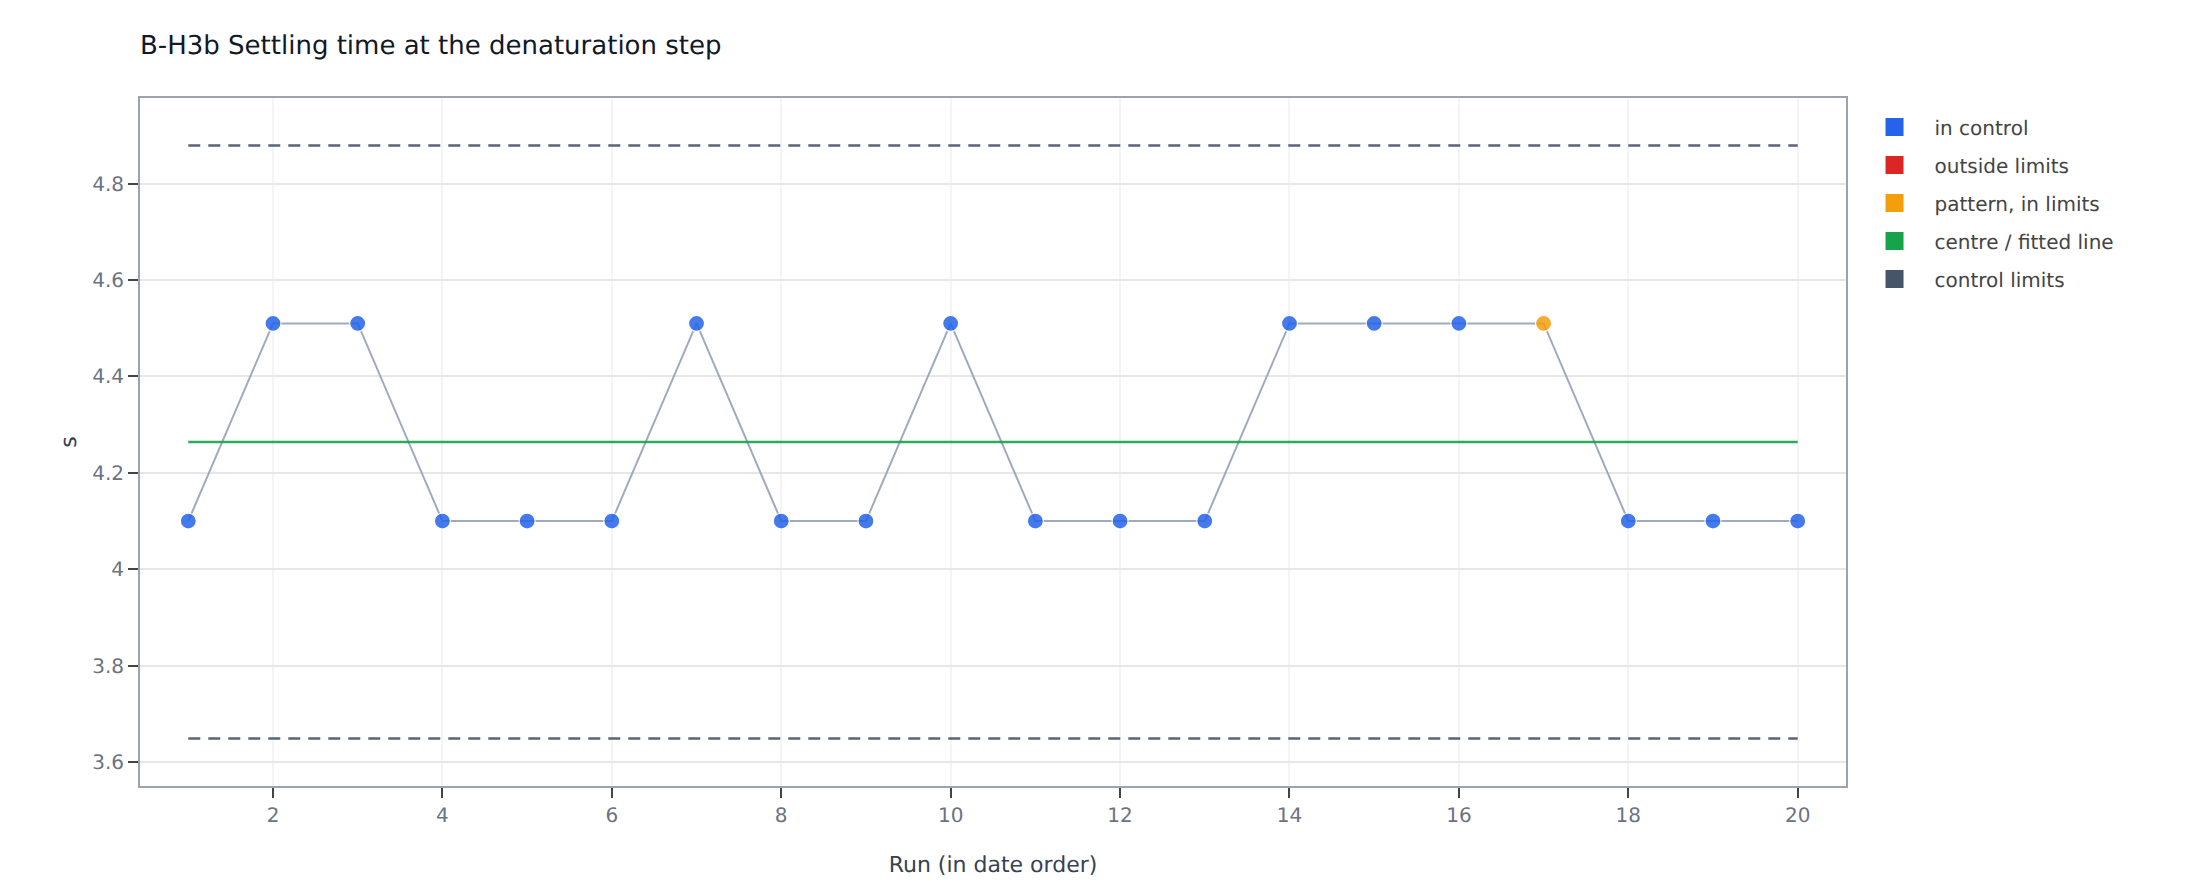
\includegraphics[width=0.92\linewidth,height=0.80\textheight,keepaspectratio]{fig/gallery/s9_alarm_2.png}
\caption[B-H3b Settling time at the denaturation step — out of control --- 1 flagged point(s): signal in the last 5 runs]{\synthtag B-H3b Settling time at the denaturation step — out of control --- 1 flagged point(s): signal in the last 5 runs. {\footnotesize Exercises \texttt{ccChartSvg}, \texttt{ccCompute}, \texttt{ccStatus}, \texttt{ccWestgard} and 38 more function(s) reachable from them.}}
\label{fig:gal-s9-alarm-2}
\end{figure}

\begin{figure}[H]\centering
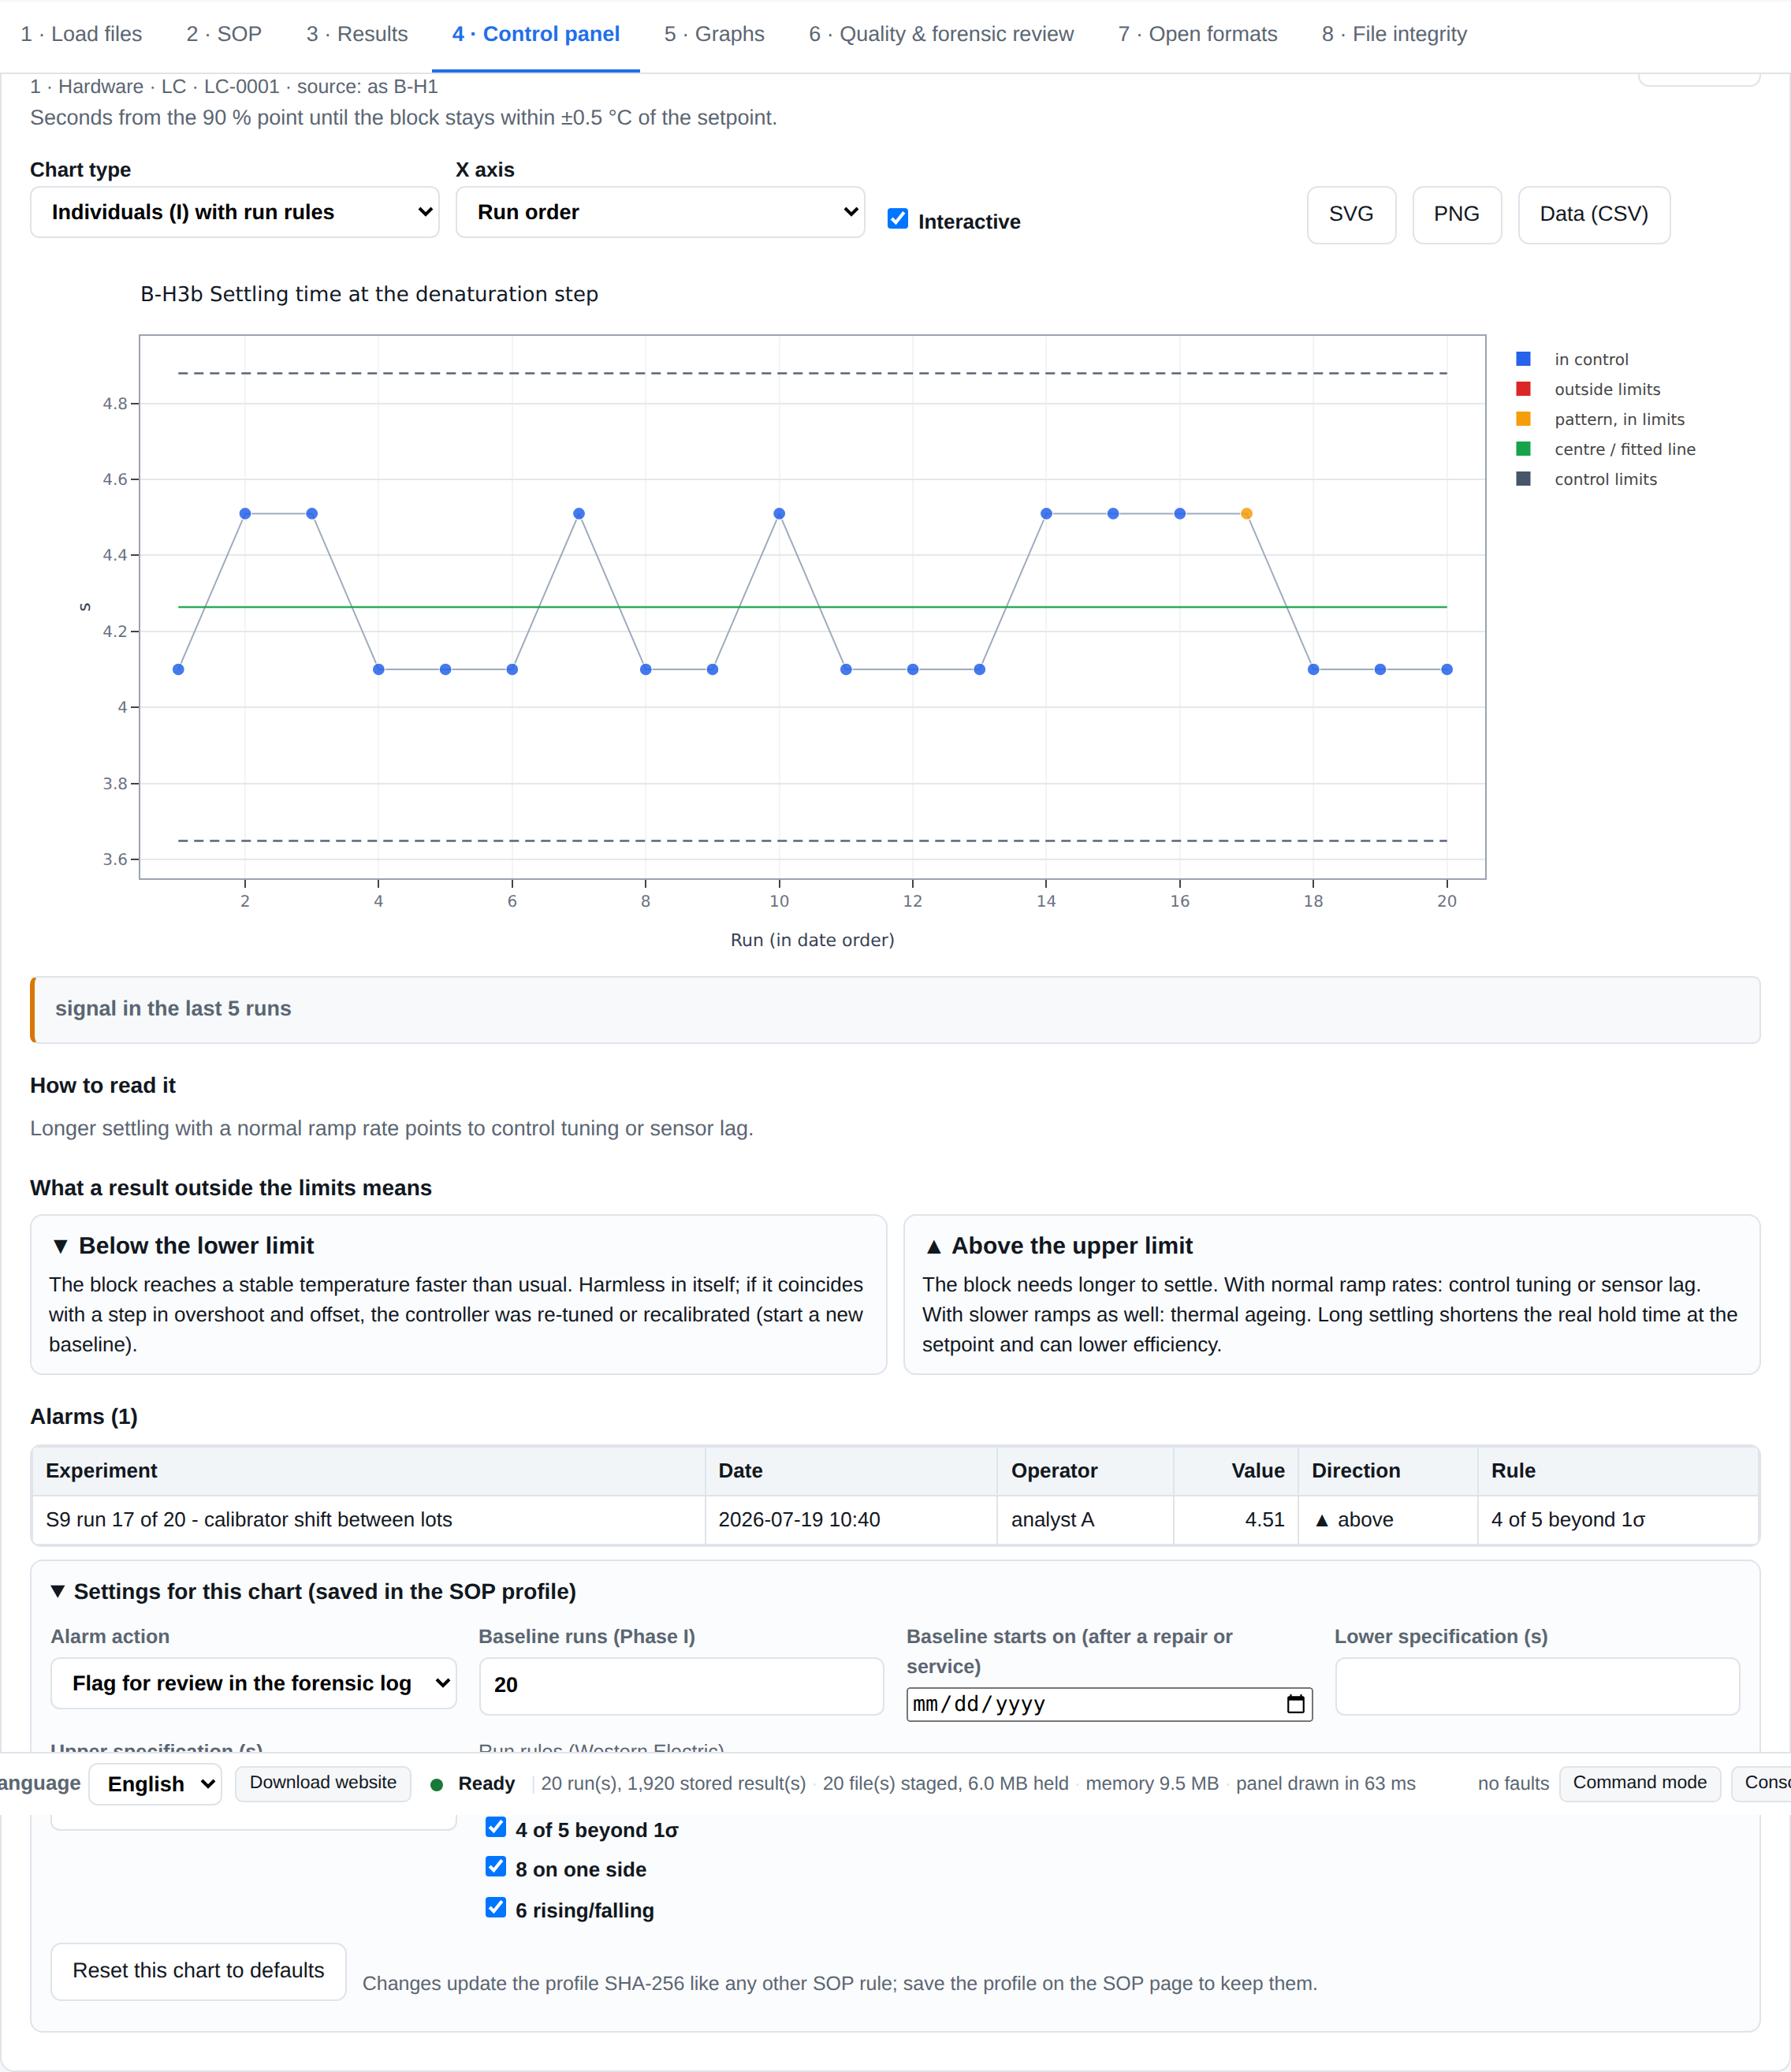
\includegraphics[width=0.92\linewidth,height=0.80\textheight,keepaspectratio]{fig/gallery/s9_alarm_2_card.png}
\caption[The alarm record for B-H3b Settling time at the denaturation step --- signal in the last 5 runs]{\synthtag The alarm record for B-H3b Settling time at the denaturation step --- signal in the last 5 runs. {\footnotesize Exercises \texttt{ccAlarmDir}, \texttt{ccChartRows}, \texttt{ccStatus}, \texttt{renderCcDetail} and 129 more function(s) reachable from them.}}
\label{fig:gal-s9-alarm-2-card}
\end{figure}

\subsection*{The same values, a different statistic}
A step of this size is what CUSUM and EWMA are for: the individuals chart may hold its limits while the accumulated deviation does not.

\begin{figure}[H]\centering
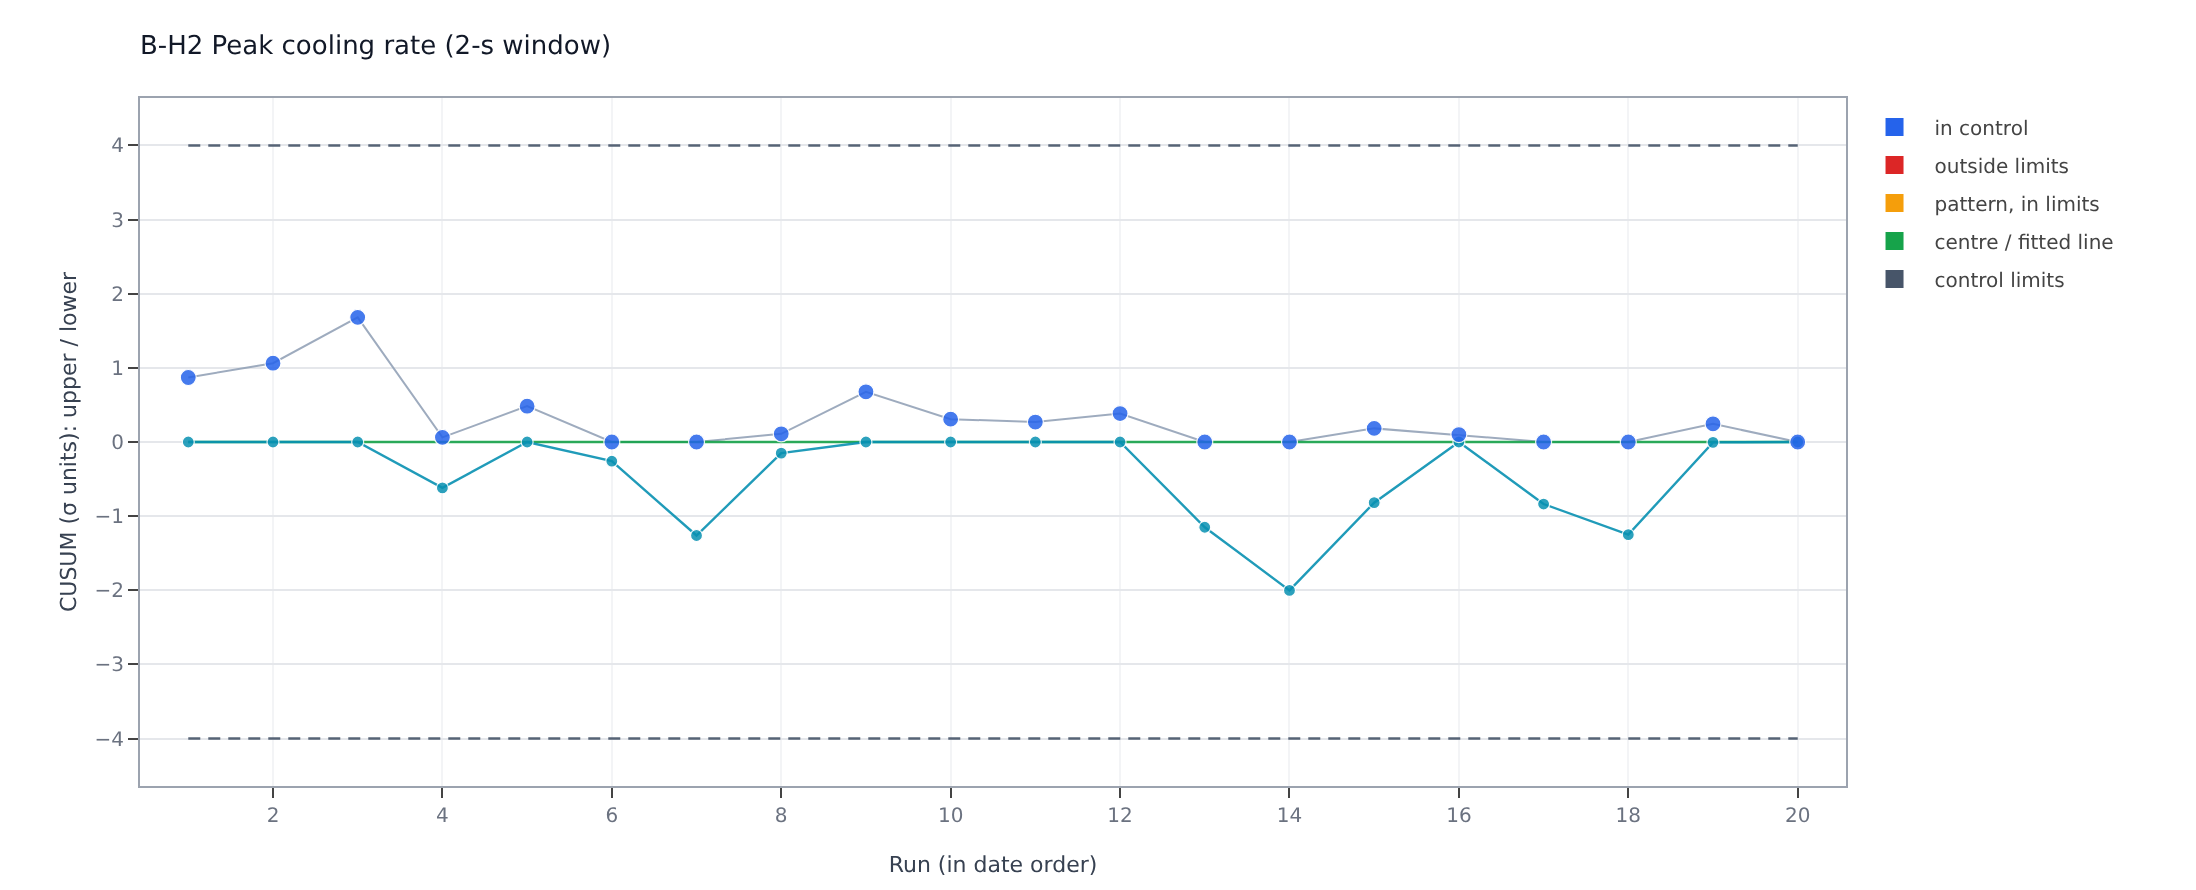
\includegraphics[width=0.92\linewidth,height=0.80\textheight,keepaspectratio]{fig/gallery/s9_cusum.png}
\caption[B-H2 Peak cooling rate (2-s window) read as a cusum chart --- the same values, a different statistic]{\synthtag B-H2 Peak cooling rate (2-s window) read as a cusum chart --- the same values, a different statistic. {\footnotesize Exercises \texttt{ccChartSvg}, \texttt{ccCompute} and 38 more function(s) reachable from them.}}
\label{fig:gal-s9-cusum}
\end{figure}

\begin{figure}[H]\centering
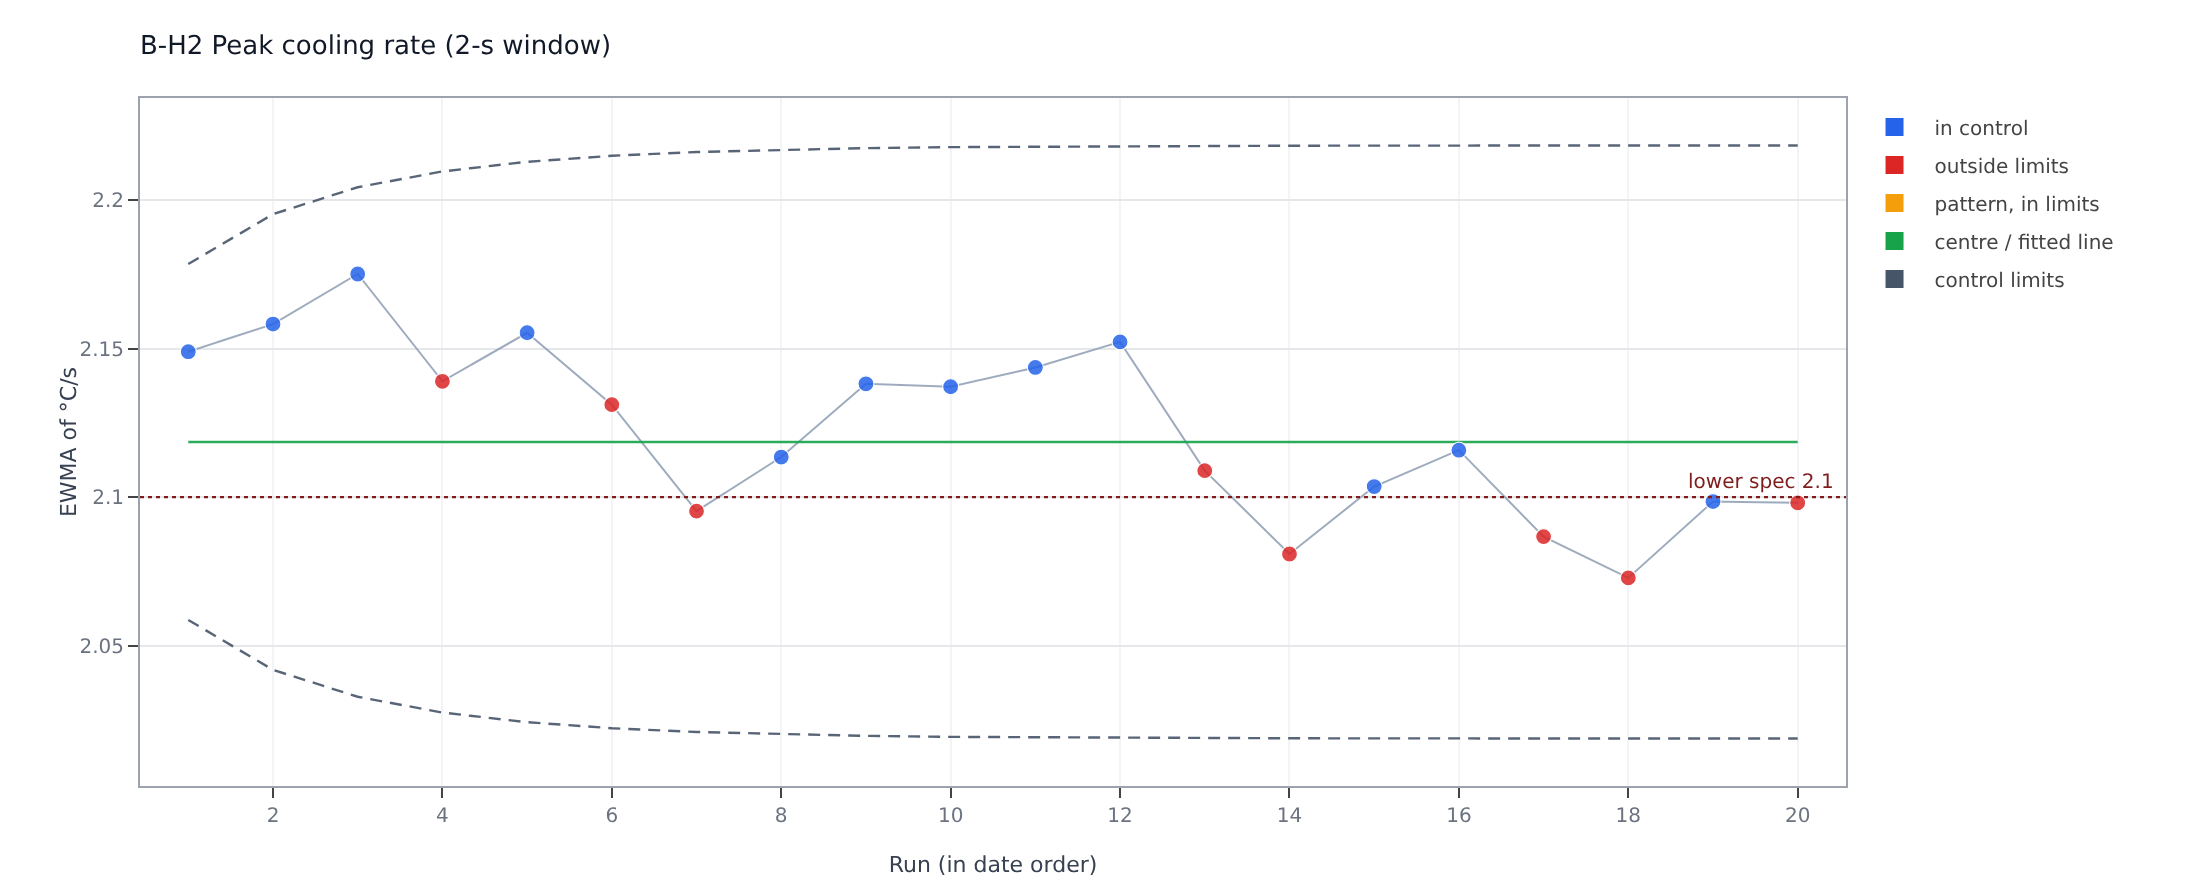
\includegraphics[width=0.92\linewidth,height=0.80\textheight,keepaspectratio]{fig/gallery/s9_ewma.png}
\caption[B-H2 Peak cooling rate (2-s window) read as a ewma chart --- the same values, a different statistic]{\synthtag B-H2 Peak cooling rate (2-s window) read as a ewma chart --- the same values, a different statistic. {\footnotesize Exercises \texttt{ccChartSvg}, \texttt{ccCompute} and 38 more function(s) reachable from them.}}
\label{fig:gal-s9-ewma}
\end{figure}

\begin{figure}[H]\centering
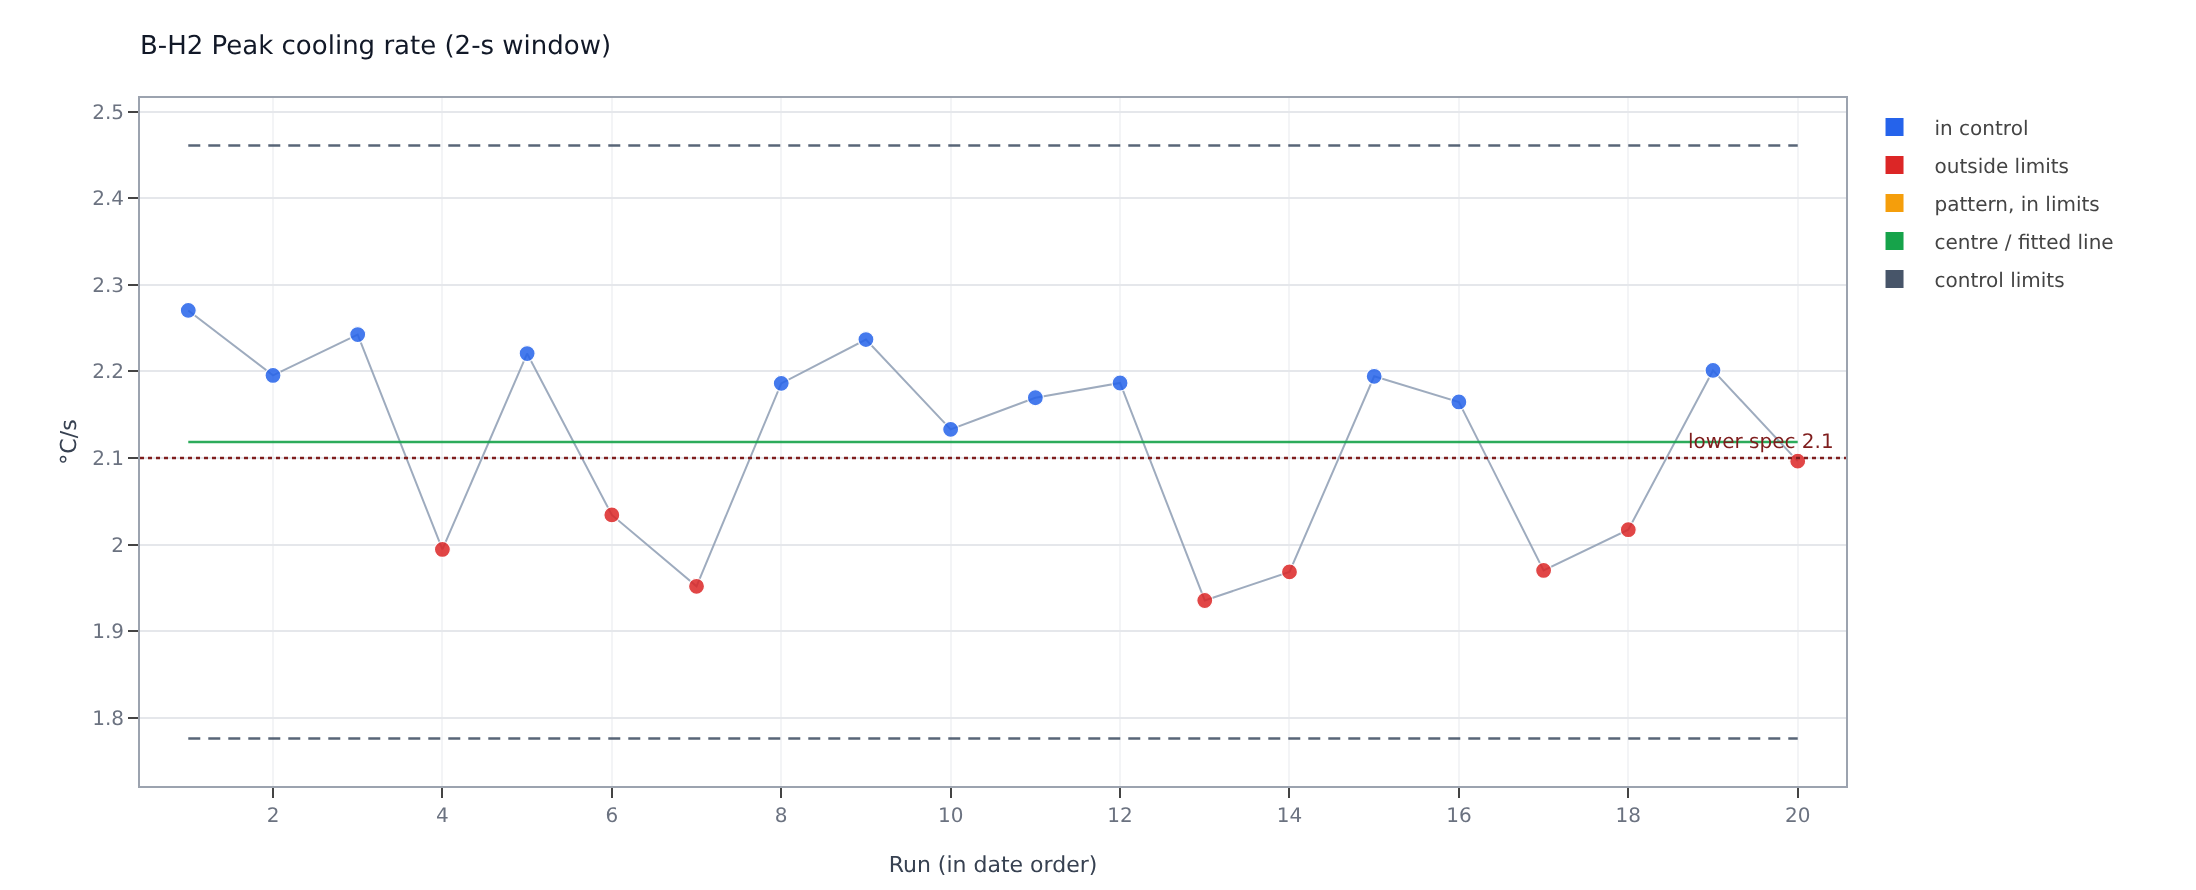
\includegraphics[width=0.92\linewidth,height=0.80\textheight,keepaspectratio]{fig/gallery/s9_trend.png}
\caption[B-H2 Peak cooling rate (2-s window) read as a trend chart --- the same values, a different statistic]{\synthtag B-H2 Peak cooling rate (2-s window) read as a trend chart --- the same values, a different statistic. {\footnotesize Exercises \texttt{ccChartSvg}, \texttt{ccCompute} and 38 more function(s) reachable from them.}}
\label{fig:gal-s9-trend}
\end{figure}

\subsection*{What the rest of the page says about the same runs}
\begin{figure}[H]\centering
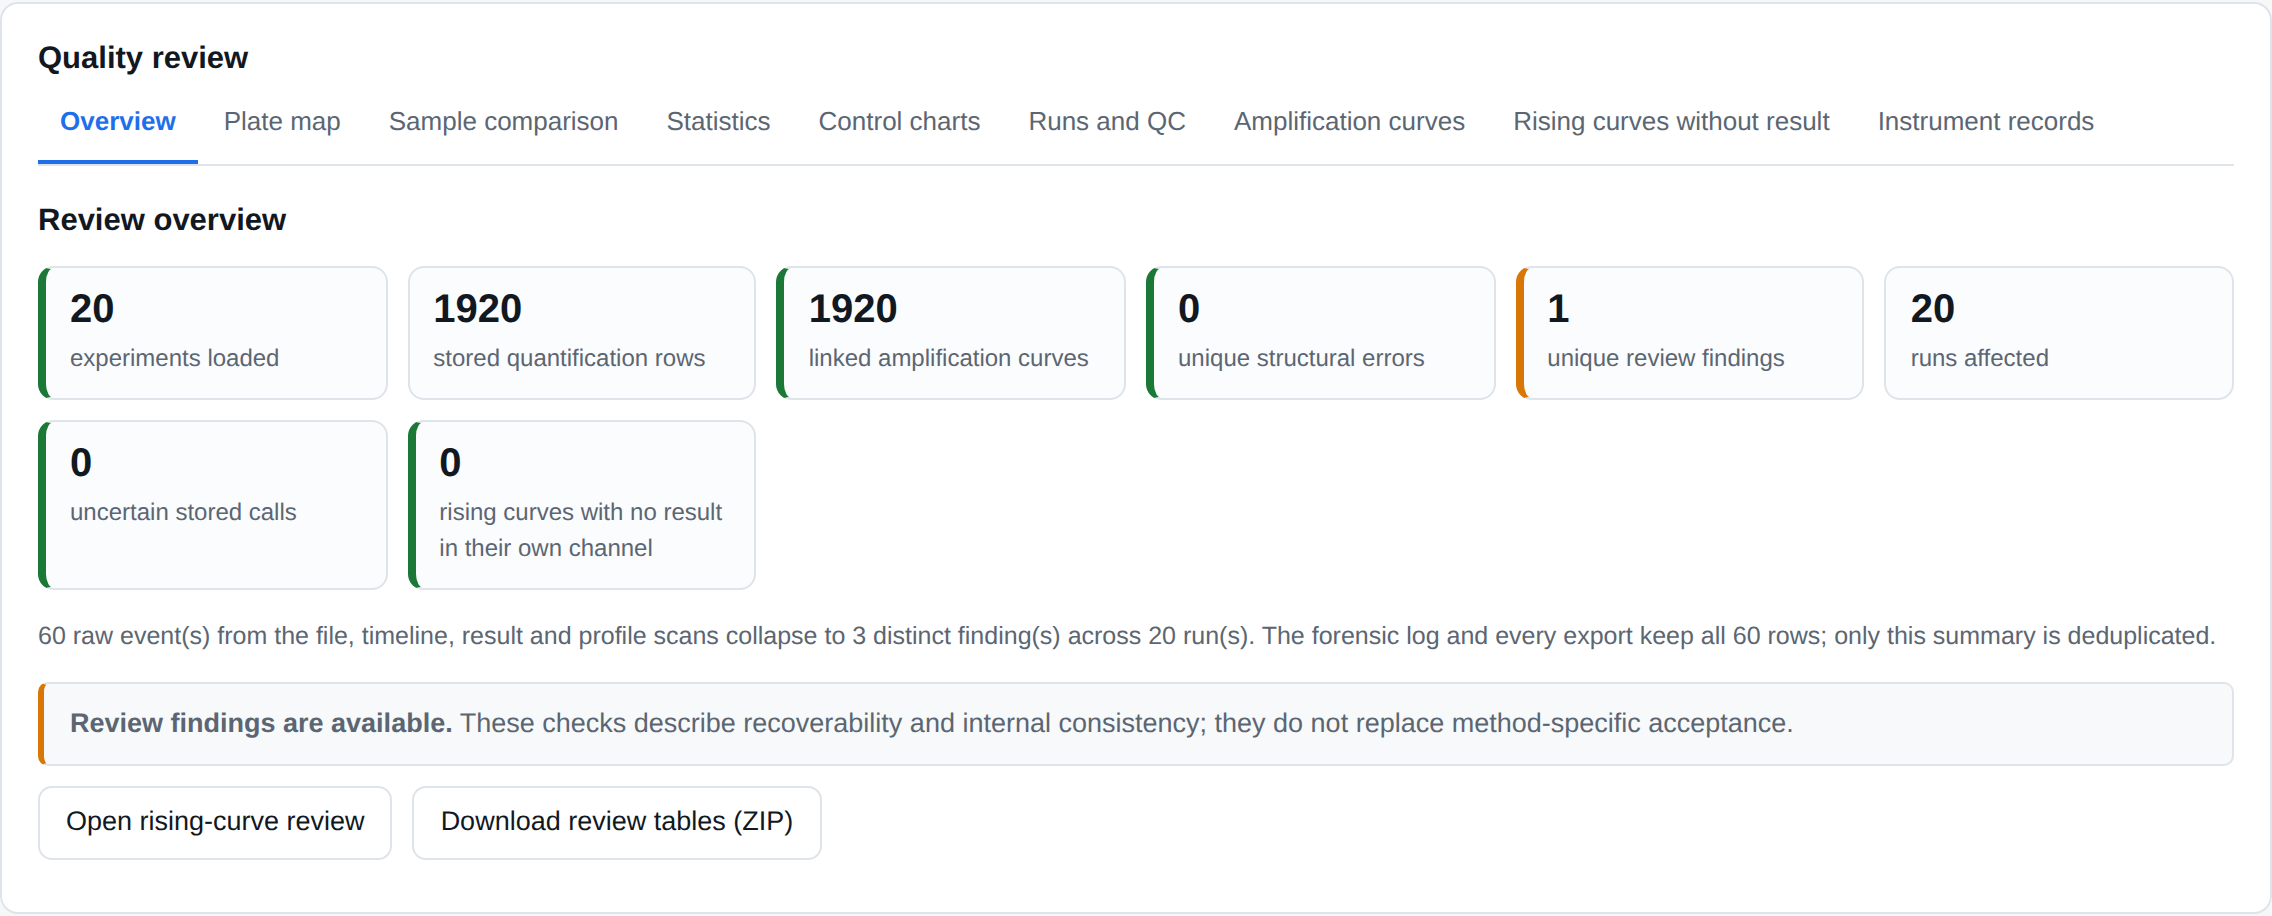
\includegraphics[width=0.92\linewidth,height=0.80\textheight,keepaspectratio]{fig/gallery/s9_review.png}
\caption[The forensic review of the same twenty runs]{\synthtag The forensic review of the same twenty runs. {\footnotesize Exercises \texttt{currentReviewSheet}, \texttt{renderReviewSheetLazy}, \texttt{reviewForensicEvents}, \texttt{reviewRunRows} and 231 more function(s) reachable from them.}}
\label{fig:gal-s9-review}
\end{figure}

\begin{figure}[H]\centering

\includegraphics[width=0.92\linewidth,height=0.80\textheight,keepaspectratio]{fig/gallery/s9_graph_x_control.png}
\caption[Control Cq across runs, with the step at run 9]{\synthtag Control Cq across runs, with the step at run 9. {\footnotesize Exercises \texttt{controlBatchGraph}, \texttt{controlBatchRecords}, \texttt{extent}, \texttt{gByDate}, \texttt{gCutLines}, \texttt{gRunTicks} and 69 more function(s) reachable from them.}}
\label{fig:gal-s9-graph-x-control}
\end{figure}

\begin{figure}[H]\centering
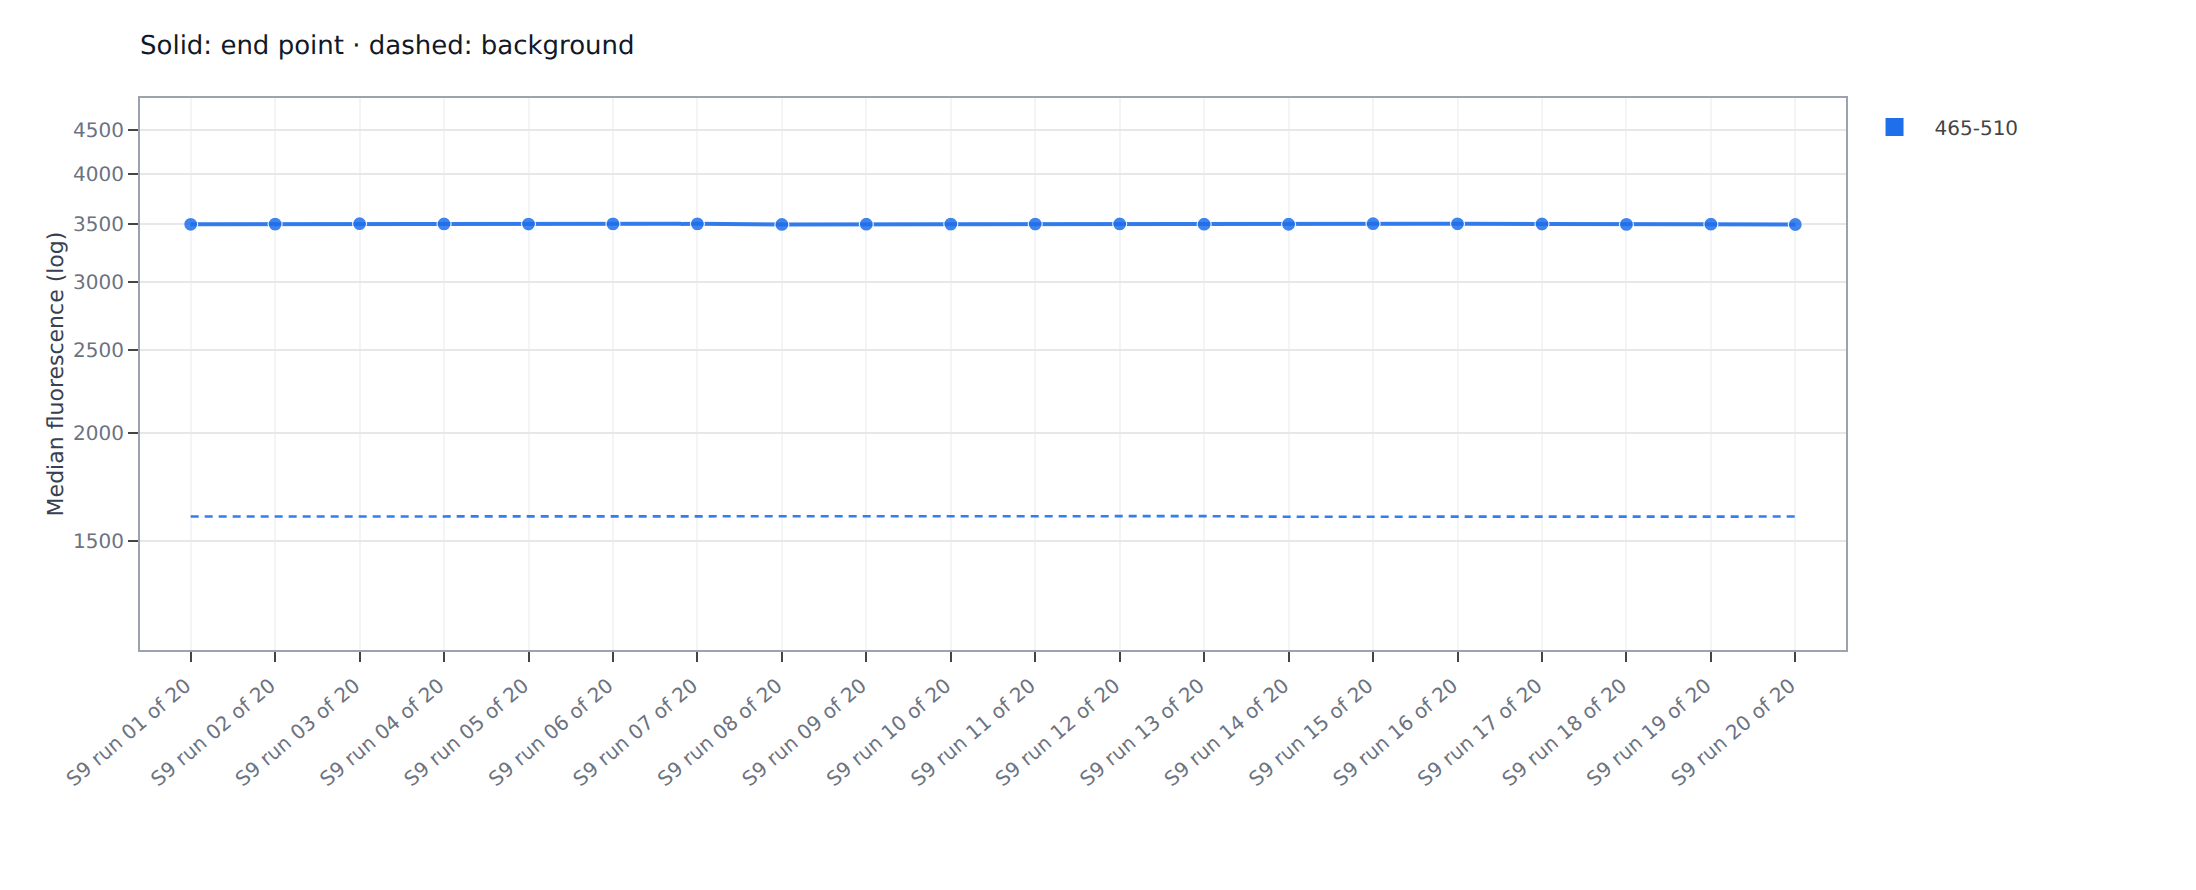
\includegraphics[width=0.92\linewidth,height=0.80\textheight,keepaspectratio]{fig/gallery/s9_graph_x_signal.png}
\caption[Background and plateau fluorescence across the series]{\synthtag Background and plateau fluorescence across the series. {\footnotesize Exercises \texttt{extent}, \texttt{gByDate}, \texttt{gCutLines}, \texttt{gRunTicks}, \texttt{gRunWells}, \texttt{gTargets} and 56 more function(s) reachable from them.}}
\label{fig:gal-s9-graph-x-signal}
\end{figure}

\begin{figure}[H]\centering
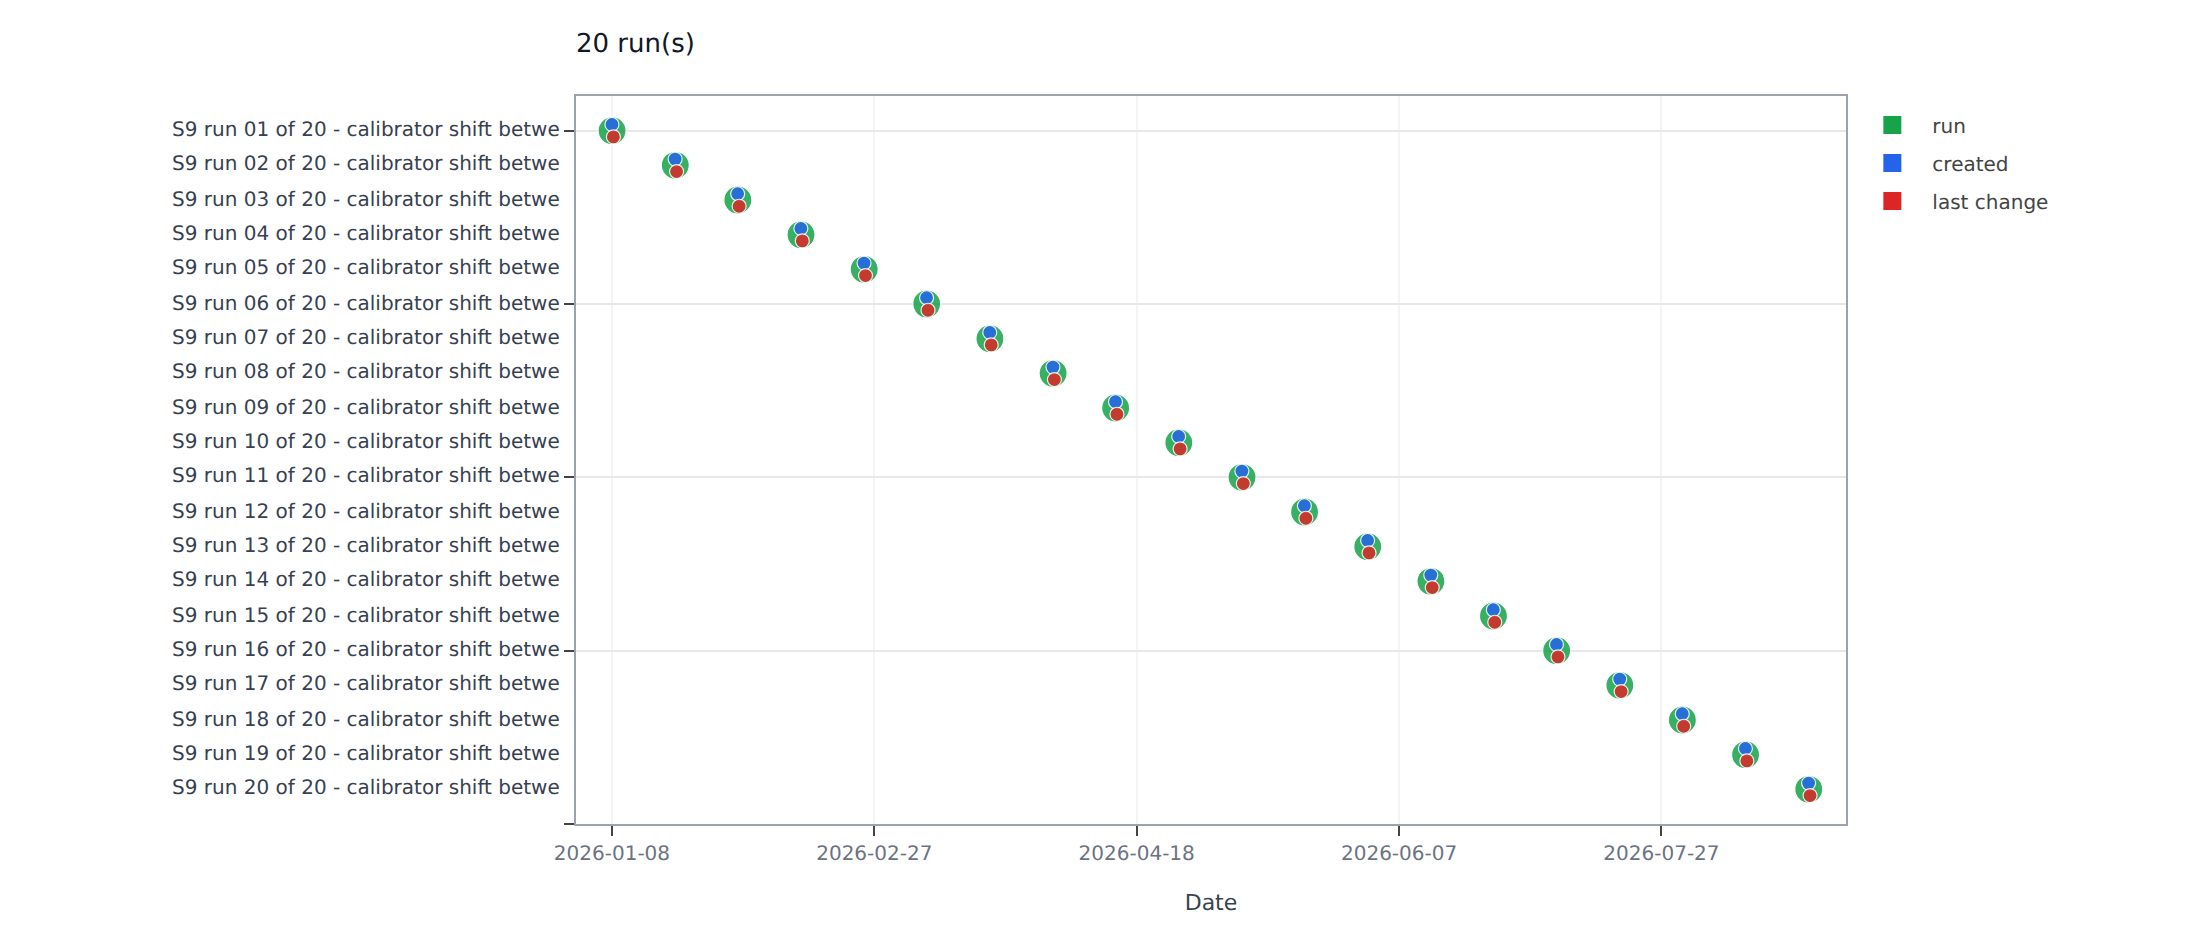
\includegraphics[width=0.92\linewidth,height=0.80\textheight,keepaspectratio]{fig/gallery/s9_graph_x_timeline.png}
\caption[The twenty runs on a calendar]{\synthtag The twenty runs on a calendar. {\footnotesize Exercises \texttt{extent}, \texttt{gByDate}, \texttt{gCutLines}, \texttt{gRunTicks}, \texttt{gRunWells}, \texttt{gTargets} and 56 more function(s) reachable from them.}}
\label{fig:gal-s9-graph-x-timeline}
\end{figure}

\section{The interactive view}
\begin{figure}[H]\centering
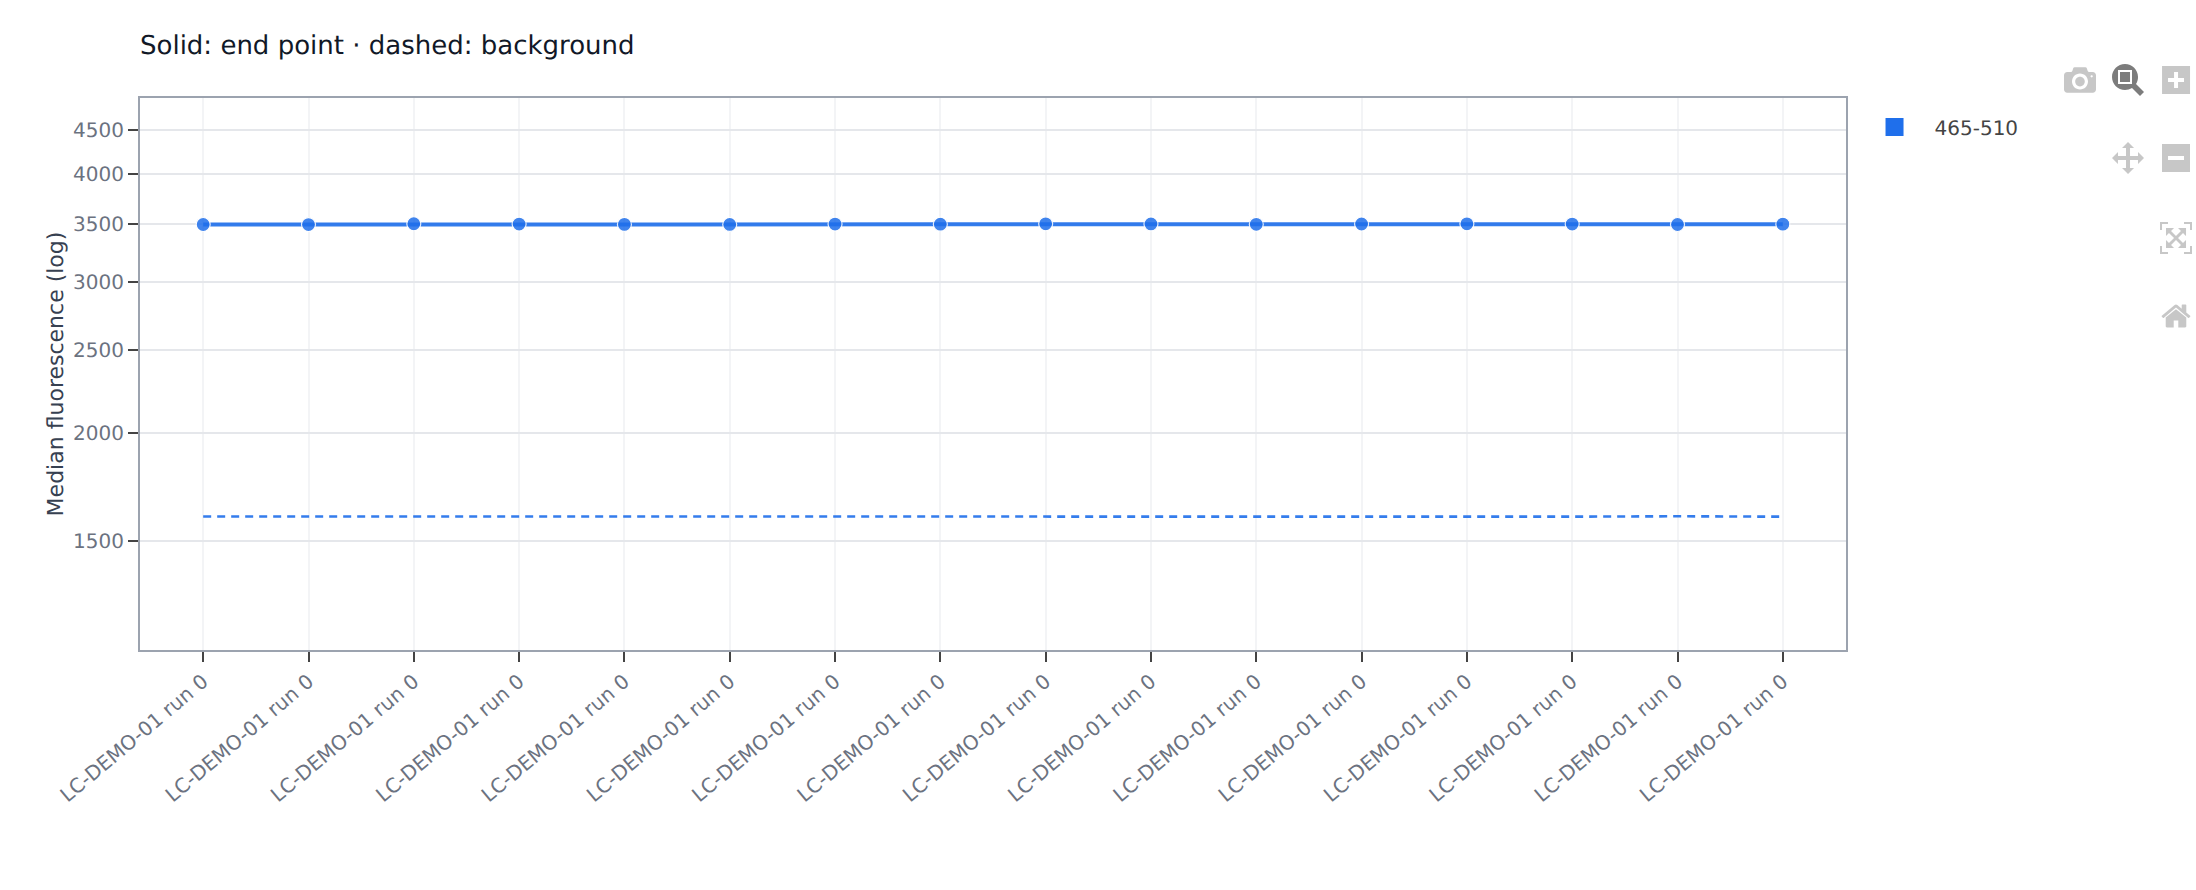
\includegraphics[width=0.96\linewidth,height=0.80\textheight,keepaspectratio]{fig/gallery/interactive_figure.png}
\caption[A chart as an interactive figure, with its toolbar --- the drawn SVG stays in the page for every download]{\synthtag A chart as an interactive figure, with its toolbar --- the drawn SVG stays in the page for every download. {\footnotesize Exercises \texttt{ixLayout}, \texttt{ixMount}, \texttt{ixTraces}, \texttt{renderGraphs} and 22 more function(s) reachable from them.}}
\label{fig:gal-interactive-figure}
\end{figure}

